\chapter{Probability by Rosenthal }
In this chapter, I will include sporadic notes during my study of probability from the Rosenthal book. Also, I will try to compile a set of solutions for the problems in this book.



\section{Probability Triples}

\begin{definition}[Semialgebra]
	Let $ X $ be a set. A Semialgebra $ \mathcal{I} $ of the subsets of $ X $ is a collection of the subsets of such that 
	\begin{enumerate}[(a)]
		\item $ \emptyset, X \in \mathcal{I} $.
		\item $ \mathcal{I} $ is closed \emph{finite} \textbf{intersection}.
		\item For $ E \in \mathcal{I} $ it complement $ E^c $ can be written as a \emph{finite disjoint} \textbf{union} of sets in $ \mathcal{I} $.
	\end{enumerate}
\end{definition}
\begin{remark}
	One canonical example for a semialgebra is the set of all intervals in $ \R $, where the term interval contains all open, closed and half open intervals, as well as the empty set, singletons, and the whole space. 
\end{remark}

\begin{definition}[Algebra]
	Let $ \mathcal{M} $ be a collection of sets. Then $ \mathcal{M} $ is an algebra if 
	\begin{enumerate}[(a)]
		\item $ \Omega, \emptyset \in \mathcal{M} $
		\item $ \mathcal{M} $ is closed under complements.
		\item $ \mathcal{M} $ is closed under finite intersection.
		\item $ \mathcal{M} $ is closed under finite union.
	\end{enumerate}
\end{definition}

\begin{proposition}
	Let $ \mathcal{I} $ be a semialgebra, and $ \mathcal{F} = \sigma(\mathcal{I}) $. Let $ \mathbb{P},\mathbb{Q} $ be two probability measures defined on $ \mathcal{F} $. Then if $ \mathbb{P} $ agrees with $ \mathbb{Q} $ on $ \mathcal{I} $, then they agree on $ \mathcal{F} $.
\end{proposition}
\begin{remark}
	The condition that $ \mathcal{I} $ is a semialgebra is crucial. See \autoref{prob:BeingSemiAlgebraIsImportant} for an example.
\end{remark}


\newpage

\subsection{Solved Problems}
\begin{problem}
	Let $ \Omega = \set{1,.2,3,4} $. Determine whether or not each of the following is a $\sigma\text{-algebra}$.
	\begin{enumerate}[(a)]
		\item $ \mathcal{F}_1 = \set{\emptyset, \set{1,2},\set{3,4},\set{1,2,3,4}} $.
		\item $ \mathcal{F}_2 = \set{\emptyset,\set{3},\set{4},\set{1,2},\set{3,4},\set{1,2,3},\set{1,2,4},\set{1,2,3,4}} $.
		\item $ \mathcal{F}_3 = \set{\emptyset, \set{1,2},\set{1,3},\set{1,4},\set{2,3},\set{2,4},\set{3,4},\set{1,2,3,4}} $.
	\end{enumerate}
\end{problem}
\begin{solution}
	\begin{enumerate}[(a)]
		$ \, $
		\item $ \mathcal{F}_1  $ is a $\sigma\text{-algebra}$ and the set of its atoms are $ \set{\set{1,2},\set{3,4}} $. 
		\item $ \mathcal{F}_2 $ is a $\sigma\text{-algebra}$ and the set of its atoms are $ \set{\set{3},\set{4},\set{1,2}} $.
		\item $ \mathcal{F}_3 $ is \textbf{not} a $\sigma\text{-algebra}$ because $ \set{1,2},\set{2,3} \in \mathcal{F}_3 $ but $ \set{1,2}\cap\set{2,3} = \set{2} \notin \mathcal{F}_3 $.
 	\end{enumerate}
\end{solution}

\begin{problem}
	Let $ \Omega = \set{1,2,3,4} $, and let $ \mathcal{I} = \set{\set{1},\set{2}} $. Describe explicitly the $\sigma\text{-algebra}$ $ \sigma(\mathcal{I}) $ (i.e. the smallest $\sigma\text{-algebra}$ containing the collection $ \mathcal{I} $).
\end{problem}
\begin{solution}
	The smallest $\sigma\text{-algebra}$ containing the collection $ \mathcal{I} $ is
	\[ \sigma(\mathcal{I}) = \set{\set{1},\set{2},\set{3,4},\set{1,2},\set{2,3,4},\set{1,3,4},\set{1,2,3,4},\emptyset}. \]
	One way to check to see if this is really the smallest $\sigma\text{-algebra}$ is to first observe that the cardinality of $\sigma\text{-algebra}$ of a finite set should always be of the form $ 2^n $ for some $ n \in \N $, where $ n $ is the number of atoms (or the number of the non-empty sets the the $\sigma\text{-algebra}$ does not contain any of its subsets). Observe that $ \set{1} $ and $ \set{2} $ are already the atoms of the $\sigma\text{-algebra}$. Thus the size of $ \sigma(\mathcal{I}) $ must be at least four. However, we know that $ \sigma(\mathcal{I}) $ contains at least $ 5 $ elements (i.e. $ \set{1},\set{2},\set{1,2},\set{1,2,3,4},\emptyset $). This suggests that there should be at least one other atom in the set. Choosing that atom to be $ \set{3,4} $ will yield that $ \sigma(\mathcal{I}) $ that contains $ 8 $ elements. Since this already includes that collection $ \mathcal{I} $, and we can not have any smaller $\sigma\text{-algebra}$ then we are sure that this is the smallest $\sigma\text{-algebra}$.
\end{solution}


\begin{problem}
	Suppose $ \mathcal{F} $ is a collection of subsets of $ \Omega $, such that $ \Omega \in \mathcal{F} $.
	\begin{enumerate}[(a)]
		\item Suppose $ \mathcal{F} $ is an algebra. Prove that $ \mathcal{F} $ is a semialgebra.
		\item Suppose that whenever $ A,B \in \mathcal{F} $, then also $ A\backslash B \equiv A \cap B^c \in \mathcal{F} $. Prove that $ \mathcal{F} $ is an algebra. 
		\item Suppose that $ \mathcal{F} $ is closed under complement, and also closed under finite \emph{disjoint} unions. Give a counter example to show that $ \mathcal{F} $ might not be an algebra. 
	\end{enumerate}
\end{problem}

\begin{solution}
	\begin{enumerate}[(a)]
		\item Firstly, Since $ \mathcal{F} $ is an algebra, then it is closed under complement, hence $ \emptyset \in \mathcal{F} $. Secondly, Since it is closed under finite intersection, then it meets the closedness under finite intersection property of a semialgebra. Lastly, let $ E \in \mathcal{F} $. Since $ \mathcal{F} $ is an algebra then $ E^c \in \mathcal{F} $. So we can trivially write $ E^c = E^c $ as a finite disjoint union of sets in $ \mathcal{F} $. Thus $ \mathcal{F} $ is a semialgebra.
		\item Firstly, since $ \Omega \in \mathcal{F} $, then by hypothesis $ \Omega \backslash \Omega = \emptyset \in \mathcal{F} $. Secondly, let $ A \in \mathcal{F} $. Then by hypothesis $ \Omega \ A = A^c \in \mathcal{F} $, thus $ \mathcal{F} $ is closed under complement. Lastly, Let $ A,B \in \mathcal{F} $. By the reasoning above $ B^c \in \mathcal{F} $. And by hypothesis $ A\backslash B^c \in \mathcal{F} $. This implies that $ A \cap B \in \mathcal{F} $
		\item One simple counter example can be constructed when we let $ \Omega = \set{1,2,3,4} $ and then let 
		\[ \mathcal{F} = \set{\Omega,\emptyset, \set{1,2},\set{1,3},\set{1,4},\set{2,3},\set{2,4},\set{3,4}}. \]
		This collection is closed under finite disjoint union as well as complement. But it fails to be an algebra. For instance $ \set{1,2},\set{2,3} \in \mathcal{F} $, but their intersection is not in the collection.
	\end{enumerate}
\end{solution}

\begin{problem}
	Let $ \mathcal{F}_1,\mathcal{F}_2,\cdots $ be a sequence of collections of subsets of $ \Omega $, such that $ \mathcal{F}_n \subseteq \mathcal{F}_{n+1} $ for each $ n $. 
	\begin{enumerate}[(a)]
		\item Suppose that each $ \mathcal{F}_i $ is an algebra. Prove that $ \bigcup_{i=1}^\infty \mathcal{F}_i $ is also an algebra. 
		\item Suppose that each $ \mathcal{F}_i $ is a $\sigma\text{-algebra}$. Show (by counterexample) that $ \bigcup_{i=1}^\infty  \mathcal{F}_i$ need not be a $\sigma\text{-algebra}$.
	\end{enumerate}
\end{problem}
\begin{solution}
	\begin{enumerate}[(a)]
		\item Let $ \mathcal{G} = \bigcup_{i=1}^\infty \mathcal{F}_i $. First, observe that since $ \Omega, \emptyset \in \mathcal{F}_i $ for all $ i\in \N $ (since all of them are algebra), then it follows that $ \Omega, \emptyset \in \mathcal{G} $. Furthermore, let $ A \in \mathcal{G} $. Then $ A \in \mathcal{F}_i $ for some $ i\in\N $. Since $ \mathcal{F}_i $ is an algebra, then $ A^c \in \mathcal{F}_i $, hence $ A^c \in \mathcal{G} $. Lastly, let $ A,B \in \mathcal{G} $. Then $ A\in\mathcal{F}_i $ and $ B \in \mathcal{F}_j $ for some $ i,j \in \N $. WLOG we can assume $ i \leq j $. Then $ \mathcal{F}_i \subset \mathcal{F}_j $, hence $ A,B \in \mathcal{F}_j $. Since $ \mathcal{F}_j $ is an algebra, then $ A\cap B \in \mathcal{F}_j $. Thus $ A \cap B \in \mathcal{G} $. This proves that $ \mathcal{G} $ is an algebra. 
		\item Let $ \Omega = \N $. Let $ \mathcal{F}_n $ be the smallest $\sigma\text{-algebra}$ that contains the collection $ \set{\set{1},\cdots,\set{n}} $. On other way to think about $ \mathcal{F}_n $ is the $\sigma\text{-algebra}$ that contains the power set of $ \set{1,\cdots,n} $ as well as all of their complements (with respect to $ \Omega $). For instance, we have
		\[ \mathcal{F}_1 = \set{\emptyset,\set{1},\N, \set{1}^c}. \]
		Similarly
		\[ \mathcal{F}_2 = \set{\emptyset,\set{1},\set{2},\set{1,2},\N,\set{1}^c,\set{2}^c,\set{1,2}^c}, \]
		and etc. Let $ A_i = \set{2 i} $. Clearly $ A_i \in \bigcup_i \mathcal{F}_i $. However, $ \bigcup_i A_i \notin \bigcup_i \mathcal{F}_i$ as it does not belong to any $ \mathcal{F}_k $. Thus $ \bigcup_i\mathcal{F}_i $ is not a $\sigma\text{-algebra}$.
	\end{enumerate}
\end{solution}

\begin{problem}
	Suppose that $ \Omega = \N  $ is the set of positive integers, and $ \mathcal{F} $ is the set of all subsets $ A $ such that either $ A $ or $ A^c $ is finite, and $ \prob $ is defined by $ \prob(A) = 0 $ if $ A $ is finite, and $ \prob(A) = 1 $ if $ A^c $ is finite. 
	\begin{enumerate}[(a)]
		\item Is $ \mathcal{F} $ an algebra?
		\item Is $ \mathcal{F} $ a $\sigma\text{-algebra}$?
		\item Is $ \prob $ finitely additive?
		\item Is $ \prob $ countably additive on $ \mathcal{F} $, meaning that if $ A_1,A_2,\cdots \in \mathcal{F} $ are disjoint, and if it happens that $ \bigcup_n A_n \in \mathcal{F} $, then $ \prob(\bigcup_n A_n) = \sum_n \prob(A_n) $?
	\end{enumerate}
\end{problem}
\begin{solution}
	\begin{enumerate}[(a)]
		\item Yes. First, observe that $ \emptyset, \Omega \in \mathcal{F} $ as $ \emptyset $ is finite, and $ \Omega $ has a finite complement. Further, let $ A \in \mathcal{F} $. Then either it is finite or it has a finite complement, where for both cases we have $ A^c \in \mathcal{F} $. Let $ A_1,\cdots,A_n $ be a finite collection of sets in $ \mathcal{F} $. If all $ A_i $ for $ i=1,\cdots,n $ are finite, then since the finite intersection and complement of any finite collection of finite sets is finite, $ \bigcap_{i=1}^n A_i $ as well as $ \bigcup_{i=1}^n A_i$ are finite as well, thus belongs to $ \mathcal{F} $. If $ A_i $ are all infinite, then since they all belong to $ \mathcal{F} $ then they have finite complement, hence $ \bigcup_{i=1}^n A_i^c $ and $ \bigcap_{i=1}^n A_i^c $ are finite as well, thus belongs to $ \mathcal{F} $. If the collection is not in any of the case above, then there is $ 1\leq j \leq n $ such that $ A_j $ is finite. Thus $ \bigcup_i A_i $ is finite, thus belongs to $ \mathcal{F} $. Being closed under finite intersection and complements implies being closed under finite union.
		
		\item No. Let $ A_n = \set{2n} $. Then $ A_n \in \mathcal{F} $ for all $ n\in\N $. However, $ \bigcup_n A_n \notin \mathcal{F} $ as it is neither finite nor has a finite complement.
		
		\item Yes. First observe that if $ A,B $ are both infinite with $ A^c, B^c $ finite (this $ A,B \in \mathcal{F} $), then $ A\cap B \neq\emptyset $. Otherwise, $ A^c \cup B^c = \N $ which implies that either of them is infinite which is a contradiction. Thus given $ A,B $, if both are finite then $ \prob(A\cup B) = \prob(A) + \prob(B) = 0 $ as $ A\cup B $ is also finite. If both are infinite, then based on our argument above then they are not disjoint, so the argument of additivity does not apply to them. However if WLOG $ A $ is finite and $ B $ is infinite and $ A\cap B = 0 $, then $ A\cup B $ is also infinite thus $ 1 = \prob(A\cup B) = \prob(A) + \prob(B) = 0 + 1 $.
		
		\item No. Let $ A_n = \set{n} $. Then 
		\[ \prob(\bigcup_n A_n) = \prob(\N) = 1 \neq \sum_n \prob(A_n) = 0. \]
	\end{enumerate}
	
\end{solution}

\begin{proposition}
	Let $ \Omega = \N $ and let $ \mathcal{F} $ be the collection of all subsets of $ \Omega $ that is \emph{countable} or has countable \emph{complement}. Then $ \mathcal{F} = \sigma(\mathcal{A}) $ where $ \mathcal{A} = \set{\set{1},\set{2},\cdots} $, i.e. the set of all singletons.
\end{proposition}
\begin{proof}
	Let $ E \in \mathcal{F} $. First, note that the collection $ \mathcal{F} $ is a $\sigma\text{-algebra}$. Then, notice that $ \mathcal{F} $ contain $ \mathcal{A} $ as singletons are finite, hence countable. Since $ \sigma(\mathcal{A}) $ is the smallest $\sigma\text{-algebra}$ that contain $ \mathcal{A} $ then $ \sigma(\mathcal{A})\subset \mathcal{F} $. Let $ E \in \mathcal{F} $. Then $ E $ is either countable or has a countable complement. If $ E $ is countable then it can be written as a countable union of singletons in which each singleton contains one element of $ E $. Thus $ E \in \sigma(\mathcal{A}) $. If $ E^c $ is countable, then $ E^c $ can be written as a countable union of singleton of its element. By applying De Morgan's law $ E $ can be written as a countable union of the complements of singletons (which belong to $ \sigma(\mathcal{A}) $). Thus case also implies $ E \in \sigma(\mathcal{A}) $. Thus $ \mathcal{F} = \sigma(\mathcal{A}) $.
\end{proof}

\begin{problem}
	Suppose that $ \Omega = [0,1] $ is the unit interval, and $ \mathcal{F} $ is the set of all subsets $  A $ such that either $ A $ or $ A^c $ is finite, and $ \prob $ is defined by $ \prob(A) = 0 $ of $ A $ is finite and $ \prob(A) = 1 $ if $ A^c $ is finite. 
	\begin{enumerate}[(a)]
		\item Is $ \mathcal{F} $ an algebra?
		\item Is $ \mathcal{F} $ a $\sigma\text{-algebra}$?
		\item Is $ \prob $ finitely additive?
		\item Is $ \prob $ countably additive on $ \mathcal{F} $?
	\end{enumerate}
\end{problem}

\begin{solution}
	\begin{enumerate}[(a)]
		\item Yes. Being closed under complement is immediate from the definition. Thus $ \emptyset, \Omega \in \mathcal{F} $. Let $ A,B \in\mathcal{F} $. Then if $ A,B $ are both finite, then $ A\cap B $ is also finite thus $ A\cap B \in \mathcal{F} $. If $ A,B $ are both infinite, then $ A^c, B^c $ are both finite, so it is $ A^c \cup B^c $. Being closed under complement it implies that $ A\cup B  \in \mathcal{F}$. If one of $ A,B $ is infinite and the other one is finite, then $ A \cap B $ is finite, hence $ A\cap B \in \mathcal{F} $. Thus $ \mathcal{F} $ is a $\sigma\text{-algebra}$.
		\item No. Consider the collection $ \set{A_q}_{q \in \Q} $ where $ q \in A  $. Each of these sets are finite, hence $ A_q \in \mathcal{F} $ for all $ q \in \Q $. However $ \bigcup_q A_q $ is not finite and its complement is also not finite. Thus $ \mathcal{F} $ is not closed under countable union. 
		\item Yes. First observe that if $ A,B \in \mathcal{F} $ both infinite, then their intersection can not be empty, otherwise $ A^c \cup B^c = [0,1] $ which means that at least one of them is infinite which is a contradiction. With this in mind let $ A,B \in \mathcal{F} $. If $  A,B $ both finite with empty intersection then $ 0 = \prob(A\cup B) = \prob(A) + \prob(B) = 0 + 0 $ as $ A\cup B $ is also finite. If WLOG $ A $ is infinite and $ B $ is finite and $ A\cup B = \emptyset$, then $ A\cup B $ is also infinite and we have $ 1 = \prob(A\cup B) = \prob(A) + \prob(B) = 0 + 1 $. Thus $ \prob $ is finitely additive.
		\item Yes. First observe that we can not find any two $ A,B \in \mathcal{F} $ disjoint and infinite with empty intersection since then $ A^c\cup B^c = [0,1] $ that implies at least one of them is infinite. So let $ A_1,A_2,\cdots $ be a sequence of \emph{finite} sets in $ \mathcal{F} $. Then 
		\[ 0 = \prob(\bigcup_i A_i) = \sum_i \prob(A_i) = 0. \]
		In case if just one of $ A_i $ is infinite (no more than two can be infinite at the same time) then 
		$ \bigcup_i A_i  $ is infinite and 
		\[ 1 = \prob(\bigcup_i A_i) = \sum_i \prob(A_i) = 1.  \]
	\end{enumerate}
\end{solution}

\begin{problem}
	\label{prob:countableAdditivityOfProbabilityOnSigmaAlg}
	Suppose that $ \Omega =[0,1] $ is the unit interval, and $ \mathcal{F} $ is the set of all subsets $ A $ such that either $ A $ or $ A^c $ is countable (i.e. finite or countable), and $ \prob $ is defined by $ \prob(A) =0 $ if $ A $ is countable, and $ \prob(A) = 1 $ if $ A^c $ is countable.
	\begin{enumerate}[(a)]
		\item Is $ \mathcal{F} $ an algebra?
		\item Is $ \mathcal{F} $ a $\sigma\text{-algebra}$?
		\item Is $ \prob $ finitely additive?
		\item Is $ \prob $ countably additive?
	\end{enumerate}
\end{problem}
\begin{solution}
	\begin{enumerate}[(a)]
		\item Yes. Being closed under complement follows immediately from the definition. On the other hand, since $ \emptyset $ is finite, then $ \Omega $ (complement of the empty set) also belongs to $ \Omega $.  Let $ A,B \in \mathcal{F} $. If both are countable then $ A\cap B $ is also countable, thus $ A\cap B \in \mathcal{F} $. If for both their complement is countable, then $ A^c \cup B^c = (A\cap B)^c $ is countable. Thus $ A\cap B \in \mathcal{F} $. If one of them is countable, WLOG $ A $, then $ A\cap B $ is also countable, thus $ A\cap B \in \mathcal{F} $. Thus it is an algebra.  
		\item Yes. Being closed under complement follows from the definition and from this it follows that $ \Omega \in \mathcal{F} $. Let $ E_1,E_2,\cdots $ be a sequence of sets in $ \mathcal{F} $. If at least one of them is countable, then $ \bigcap_i E_i $ is also countable hence belonging to $ \mathcal{F} $. If all is uncountable, then $ \bigcup_i E^c_i $ is countable. We can write $ \bigcup_i E^c_i = (\bigcap_i E_i)^c $ that is finite. Thus $ \bigcap+i E_i \in \mathcal{F} $. This shows that $ \mathcal{F} $ is closed under countable union. Being closed under union follows from being closed under intersection and complement. Thus $ \mathcal{F} $ is a $\sigma\text{-algebra}$.
		\item Yes. We will show additivity for two sets and finite additivity will follow by induction. Let $ A,B \in \mathcal{F} $. If $ A,B $ both are disjoint countable then $ A\cup B $ is also countable. Thus $ 0= \prob(A\cup B) = \prob(A) + \prob(B) = 0+0 = 0 $. If $ A, B $ are both uncountable (i.e. $ A^c, B^c $ are countable) then $ A\cap B $ can not be non-empty, otherwise $ A^c\cup B^c = [0,1] $ which then implies that at least one of $ A^c $ or $ B^c $ be uncountable, which is a contradiction. When one of these sets is countable, WLOG $ A $, then $ A\cup B $ is also uncountable and we have $ 1 = \prob(A\cup B) = \prob(A) + \prob(B) = 1 + 0 $. Thus $ \prob $ is finitely countable.
		\item Yes. Let $ A_1,A_2,\cdots $ be a sequence of disjoint sets in $ \mathcal{F} $. Then at most one set can be uncountable, otherwise they will fail to be disjoint (see the reasoning in part (c)). If non of them are uncountable, then their union is also countable (countable union of countable sets is countable). Thus $ 0 = \prob(\bigcup_i A_i) = \sum_i \prob(A_i) = 0 $. If one of them is uncountable, then the union is also uncountable and we will have $ 1 = \prob(\bigcup_i A_i) = \sum_i \prob(A_i) = 0 +\cdots + 0 + 1 + 0 + \cdots = 1 $. Thus $ \prob $ is additive on $ \mathcal{F} $.
	\end{enumerate}
\end{solution}

\begin{problem}
	For the example of \autoref{prob:countableAdditivityOfProbabilityOnSigmaAlg}, is $ \prob $ uncountably additive?
\end{problem}
\begin{solution}
	No. Otherwise we can write $ \Omega = \bigcup_{x\in\Omega}\set{x} $. But we have
	\[ 1 = \prob(\Omega) = \sum_{x\in\Omega}\set{x} = 0. \]
\end{solution}

\begin{problem}
	Let $ \mathcal{F} $ be a $\sigma\text{-algebra}$, and write $ \abs{\mathcal{F}} $ for the total number of subsets in $ \mathcal{F} $. Prove that if $ \abs{\mathcal{F}}<\infty $, i.e. $ \mathcal{F} $  consists of just a finite number of subsets, then $ \abs{\mathcal{F}}=2^m $ for some $ m \in \N $. (\emph{Hint: Consider those non-empty subsets in $ \mathcal{F} $ which do not contain any other non-empty subset in $ \mathcal{F} $. How can all subsets in $ \mathcal{F} $ be build up from these particular subsets?}).
\end{problem}
\begin{solution}
	Let $ \mathcal{A} $ be the collection of all non-empty sets in $ \mathcal{F} $ whose non of its subsets do not belong to $ \mathcal{F} $. Then for any $ E \in \mathcal{F} $ can be build up from these ``atom'' by union. For each atom there are two possibilities to be present in the union or not. Thus there are in total $ 2^m $ elements in $ \mathcal{F} $.
\end{solution}


\begin{problem}
	\label{prob:BeingSemiAlgebraIsImportant}
	Let $ \Omega = \set{1,2,3,4} $, with $ \mathcal{F} $ the collection of all subsets of $ \Omega $. Let $ \mathbb{P} $ and $\mathbb{Q}$ be two probability measures on $ \mathcal{F} $ such that $ \mathbb{P}\set{1} = \mathbb{P}\set{2} = \mathbb{P}\set{3} = \mathbb{P}\set{4} = 1/4 $, and $ \mathbb{Q}\set{2} = \mathbb{Q}\set{4} = 1/2 $, extended to $ \mathcal{F} $ by linearity. Finally, let $ \mathcal{I}=\set{\emptyset,\Omega,\set{1,2},\set{2,3},\set{3,4},\set{1,4}} $.
	\begin{enumerate}[(a)]
		\item Prove that $ \mathbb{P}(A) = \mathbb{Q}(A) $ for all $ A \in \mathcal{I} $.
		\item Prove that there is $ A \in \sigma(\mathcal{I}) $ with $ \mathbb{P}(A) \neq \mathbb{Q}(A) $.
		\item Why does this not contradict Proposition 2.5.8 (in Rosenthal)?
	\end{enumerate}
\end{problem}
\begin{solution}
	\begin{enumerate}[(a)]
		\item By a simple calculation we can show the identity above. For instance
		\[ \mathbb{P}\set{1,2} = \mathbb{P}\set{1} + \mathbb{P}\set{2} = 1/4 + 1/4 = 1/2, \]
		where as
		\[ \mathbb{Q}\set{1,2} = \mathbb{Q}\set{1} + \mathbb{Q}\set{2} = 0 + 1/2 = 1/2. \]
		By a similar computation we can show
		\[ \mathbb{P}\set{2,3}=\mathbb{Q}\set{2,3}=1/2,\quad \mathbb{P}\set{3,4}=\mathbb{Q}\set{3,4}=1/2, \quad \mathbb{P}\set{1,4}=\mathbb{Q}\set{1,4}=1/2, \]
		and so on.
		
		\item First, observe that $ \set{1,2,3} \in \sigma(\mathcal{I}) $. That is because $ \set{3} = \set{2,3}\cap \set{3,4} \in \sigma(\mathcal{I}) $. Thus $ \set{1,2}\cup\set{3} = \set{1,2,3} \in \sigma(\mathcal{I}) $. But
		\[ \mathbb{P}\set{1,2,3} = 3/4, \qquad \mathbb{Q}\set{1,2,3} = 1/2. \]
		Thus if we let $ A = \set{1,2,3} \in \sigma(\mathcal{I}) $ then $ \mathbb{P}(A) \neq \mathbb{Q}(A) $.
		
		\item That is because the proposition 2.5.8 requires the collection $ \mathcal{I} $ be a semialgebra, which is not here. For instance $ \mathcal{I} $ is not closed under finite intersection as $ \set{1,2},\set{2,3} \in\mathcal{I} $ whereas their intersection is not in the collection.
	\end{enumerate}
\end{solution}

\begin{problem}
	Let $ (\Omega, \mathcal{M},\lambda) $ be Lebesgue measure on the interval $ [0,1] $. Let
	\[ \Omega' = \set{(x,y)\in \R^2: 0<x\leq 1, 0<y\leq 1}. \]
	Let $ \mathcal{F} $ be the collection of all subsets of $ \Omega' $ of the form
	\[ \set{(x,y)\in \R^2: x\in A, 0<y\leq 1} \]
	for some $ A \in \mathcal{M} $. Finally, defined a probability $ \mathbb{P} $ on $ \mathcal{F} $ by
	\[ \prob\set{(x,y)\in\R^2: x\in A, 0<y\leq 1} = \lambda(A). \]
	\begin{enumerate}[(a)]
		\item Prove that $ (\lambda', \mathcal{F},\prob) $ is probability space.
		\item Let $ \prob^* $ be the outer measure corresponding to $ \prob $ and $ \mathcal{F} $. Define the subset $ S \subseteq \Omega' $ by
		\[ S = \set{(x,y)\in \R^2: 0<x\leq 1, y = 1/2}. \]
		(Note that $ S \notin \mathcal{F} $.) Prove that $ \prob^*(S)=1 $ and $ \prob^*(S^c)=1 $.
	\end{enumerate}

\end{problem}
\begin{solution}
	\begin{enumerate}[(a)]
		\item $ \mathcal{F} $ being a $\sigma\text{-algebra}$ follows immediately from $ \mathcal{M} $ being a $\sigma\text{-algebra}$. To see this, for instance let $ H \in \mathcal{F} $. Then there exists some $ A \in \mathcal{M} $ such that $ H = A \times (0,1] $, where $ \times $ is the Cartesian product of two sets. Then $ H^c = \Omega'\backslash H $ will be given as $ H^c = A^c \times(0,1] $. Since $ A^c \in \mathcal{M} $ then it follows that $ H^c \in \mathcal{F} $. With a similar reasoning we can show that $ \mathcal{F} $ is a $\sigma\text{-algebra}$.
		
		\noindent Furthermore, $ \prob $ being a probability measure follows immediately from the fact that $ \lambda $ is a probability measure. For instance $ \prob(\Omega') = \lambda(\Omega) = 1 $, and $ \prob(B) \geq 0 $ for all $ B \in \mathcal{F} $ since we can write $ B = A \times(0,1] $ where $ A \in \mathcal{M} $ and by definition $ \prob(A) = \lambda(A) > 0 $. Countable additivity also follows from a similar line of reasoning.
		
		\item From the monotonicity of the outer measure and using the fact that $ S \subset \Omega' $ one gets that $ \prob^*(S) \leq \prob^*(\Omega') = \prob(\Omega') = 1 $. Furthermore, observe that we can write $ S = \Omega \times\set{1/2} $. Let $ \set{I_k \in \mathcal{F}} $ be any open cover for $ S $. Thus for each $ I_k $ there exists $ A_k \in\mathcal{M} $ such that $ I_k = A_k \times(0,1] $. Since $ S = \Omega\times\set{1/2} $ the  $ \set{B_k} $ will be an open cover for $ \Omega $. Using the fact that $ \prob(I_k) = \lambda(B_k) $
		\[ 1 = \lambda(\Omega)  \leq \sum_k \lambda(B_k) = \sum_k \prob(I_k)  \]
		Since the inequality above holds for any open cover $ \set{I_k} $ for $ S $ then we can conclude that $ 1 \leq \prob^*(S) $. So far
		\[ \prob^*(S) \geq 1, \qquad \prob^*(S)\leq 1. \]
		Then it follows that 
		\[ \prob^*(S) = 1. \]
	\end{enumerate}
\end{solution}

\begin{problem}
	\label{prob:ModifiedTHeorem}
	\begin{enumerate}[(a)]
		\item Where in the proof of Theorem 2.3.1 was assumption 2.3.3 used?
		\item How would the  of Theorem 2.3.1 be modified?
	\end{enumerate}
\end{problem}
\begin{solution}
	\begin{enumerate}[(a)]
		\item It is only used with proving the equality $ \prob(A) = \prob^*(A) $ for $ A \in \mathcal{I} $. I.e. to show that $ \prob^* $ is an extension of $ \prob $ to a larger domain $ \mathcal{M} $ which is a $\sigma\text{-algebra}$ that contain the collection $ \mathcal{I} $.
		\item Then the identity $ \prob^*(A) = \prob(A) $ for $ A \in \mathcal{I} $ should be replaced with $ \prob^*(A) \leq \prob(A) $.
 	\end{enumerate}
\end{solution}

\begin{problem}
	Let $ \Omega=\set{1,2} $, and let $ \mathcal{I} $ be the collection of all subsets of $ \Omega $, with $ \prob(\emptyset)=0, \prob(\Omega) = 1 $, and $ \prob\set{1}=\prob\set{2} = 1/3 $.
	\begin{enumerate}[(a)]
		\item Verify that all assumptions of theorem 2.3.1 other than 2.3.3 are satisfied.
		\item Verify that the assumption 2.3.3 is not satisfies.
		\item Describe precisely the $ \mathcal{M} $ and $ \prob^* $ that would result in this example from the modified version of Theorem 2.3.1 in \autoref{prob:ModifiedTHeorem}.
	\end{enumerate}
\end{problem}
\begin{solution}
	\begin{enumerate}[(a)]
		\item First, notice that the power set of $ \Omega $ finite, is always an algebra thus semialgebra. So $ \mathcal{I} $ is a semialgebra. On the other hand by the hypothesis we have $ \prob(\emptyset) = 0 $ and $ \prob(\Omega) = 1 $ which satisfies some of the conditions in Theorem 2.3.1. For the super-additivity, it holds because 
		\[ \prob(\set{1}\cup\set{2}) = 1 > \prob\set{1} + \prob\set{2} = 2/3. \]
		\item It is easy to check as $ \set{1,2},\set{1},\set{2} \in \mathcal{I} $ with $ \set{1,2} \subseteq \set{1}\cup \set{2} $ but
		\[ \prob\set{1,2} \not\leq \prob\set{1}+\prob\set{2}.\]
		\item {\color{red} \noindent TODO: TOBEADDED}
	\end{enumerate}
\end{solution}


\begin{problem}
	Let $ \Omega = [0,1] $. Let $ \mathcal{I}' $ be the set of all half-open intervals of the form $ (a,b], $ for $ 0\leq a < b \leq 1 $, togheter with the sets $ \emptyset, \Omega $, and $ \set{0} $.
	\begin{enumerate}[(a)]
		\item Prove that $ \mathcal{I}' $ is s semialgebra. 
		\item Prove that $ \sigma(\mathcal{I}') = \mathcal{B} $, i.e. that the $\sigma\text{-algebra}$ generated by this $ \mathcal{I}' $ is equal to the $\sigma\text{-algebra}$ generated by the $\sigma\text{-algebra}$ of (2.4.1) in Rosenthal.
		\item Let $ \mathcal{B}'_0 $ be the collection of all finite disjoint unions of elements of $ \mathcal{I}' $. Is $ \mathcal{B}'_0 $ the same as the algebra $ \mathcal{B}_0 $ defined in (2.2.4) Rosenthal?
	\end{enumerate}
\end{problem}
\begin{solution}
	\begin{enumerate}[(a)]
		\item By definition $ \mathcal{I}' $ contains $ \emptyset $ and $ \Omega $. To show being closed under intersection let $ A, B \in \mathcal{I}' $. If $ A,B $  are disjoint then $ A\cap B \in \mathcal{I'} $. However if $ A,B $ are not disjoint, then WLOG we can assume that $ A=(a_1,a_2], B = (b_1,b_2] $ where $ a_1 < b_1 < a_2 \leq b_2 $. Thus $ A\cap B = (b_1,a_2] $ which is also at $ \mathcal{I'} $. For the last property of a semialgebra, let $ A \in \mathcal{I'} $. We can assume $ A = (a,b] $ for $ 0\leq a<b \leq 1 $. Then $ A^c = [0,a] \cup (b,1] = \set{0}\cup (0,a] \cup (b,1] $ which is a finite disjoint union of elements of $ \mathcal{I'} $.
		\item By (2.4.1) Rosenthal, $ \mathcal{B} $ is the smallest $\sigma\text{-algebra}$ of all intervals in $ [0,1] $ where the term intervals include all open, closed, half-open, intervals as well as the empty set, singletons, and the whole set $ [0,1] $. First, notice that $ \sigma(\mathcal{I'}) $ contains all of the intervals in $ [0,1] $. That is because by using complements, countable unions, as well as countable intersections one can construct any kind of intervals using the intervals of the type $ (a,b] $. Since $ \mathcal{B} $ is the smallest $\sigma\text{-algebra}$ containing $ \mathcal{I} $ thus $ \sigma(\mathcal{I})\subseteq \sigma(\mathcal{I}') $. To show the equality,  observe that $ \mathcal{I'} \subset \mathcal{I} $ thus $ \sigma(\mathcal{I'}) \subseteq \sigma(\mathcal{I}) $. These two inequalities implies that $ \sigma(\mathcal{I'}) = \sigma(\mathcal{I}) = \mathcal{B}$. 
		\item No it is not. Since $ (1/3,1/2) \in \mathcal{B}_0 $ but not in $ \mathcal{B'}_0 $.
	\end{enumerate}
\end{solution}

\begin{problem}
	Let $ K $ be the Cantor set. Let $ D_n = K \oplus \frac{1}{n} $ be  a shifted Cantor set by $ 1/n $. Let $ B = \bigcup_n D_n $. 
	\begin{enumerate}[(a)]
		\item Draw a rough sketch of $ D_3 $.
		\item What is $ \lambda(D_3) $?
		\item Draw a rough image of $ B $.
		\item What is $ \lambda(B) $?
	\end{enumerate}
\end{problem}
\FloatBarrier
\begin{solution}
	\begin{enumerate}[(a)]
		\item See figure below.
		\item Since $ K \in \mathcal{B} $, then it is shift invariant, thus $ \lambda(K_3) = \lambda(K)  = 0 $.
		\item See the figure below.
		\item From the countable sub-additivity we have
		\[ \lambda(B) = \lambda(\bigcup_n K_n) \leq \sum_n \lambda(K_n) = 0. \]
	\end{enumerate}
	\begin{figure}[h!]
	
	
	\tikzset{every picture/.style={line width=0.75pt}} %set default line width to 0.75pt        
	
	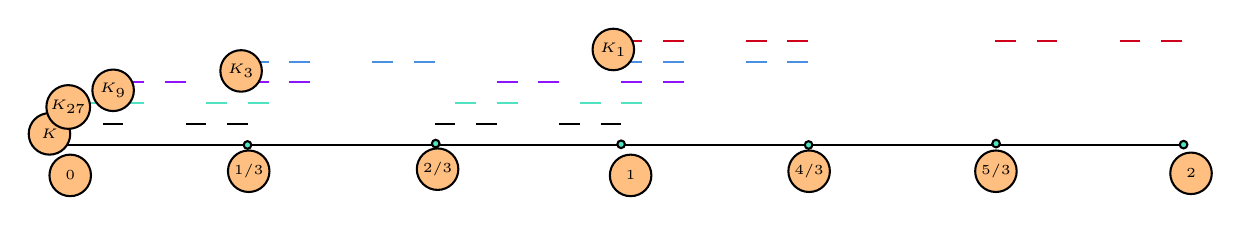
\begin{tikzpicture}[x=0.75pt,y=0.75pt,yscale=-1,xscale=1]
		%uncomment if require: \path (0,300); %set diagram left start at 0, and has height of 300
		
		%Straight Lines [id:da3663042093379123] 
		\draw    (70,160) -- (340,160) ;
		%Straight Lines [id:da30548704278309113] 
		\draw [color={rgb, 255:red, 144; green, 19; blue, 254 }  ,draw opacity=1 ][fill={rgb, 255:red, 144; green, 19; blue, 254 }  ,fill opacity=1 ]   (100,130) -- (110,130) ;
		%Straight Lines [id:da6192529867444463] 
		\draw [color={rgb, 255:red, 144; green, 19; blue, 254 }  ,draw opacity=1 ][fill={rgb, 255:red, 144; green, 19; blue, 254 }  ,fill opacity=1 ]   (120,130) -- (130,130) ;
		%Straight Lines [id:da9732533945560831] 
		\draw [color={rgb, 255:red, 144; green, 19; blue, 254 }  ,draw opacity=1 ][fill={rgb, 255:red, 144; green, 19; blue, 254 }  ,fill opacity=1 ]   (160,130) -- (170,130) ;
		%Straight Lines [id:da3271016125124977] 
		\draw [color={rgb, 255:red, 144; green, 19; blue, 254 }  ,draw opacity=1 ][fill={rgb, 255:red, 144; green, 19; blue, 254 }  ,fill opacity=1 ]   (180,130) -- (190,130) ;
		%Straight Lines [id:da21707011590164038] 
		\draw [color={rgb, 255:red, 144; green, 19; blue, 254 }  ,draw opacity=1 ][fill={rgb, 255:red, 144; green, 19; blue, 254 }  ,fill opacity=1 ]   (280,130) -- (290,130) ;
		%Straight Lines [id:da6944131266707991] 
		\draw [color={rgb, 255:red, 144; green, 19; blue, 254 }  ,draw opacity=1 ][fill={rgb, 255:red, 144; green, 19; blue, 254 }  ,fill opacity=1 ]   (300,130) -- (310,130) ;
		%Straight Lines [id:da4699188203805358] 
		\draw [color={rgb, 255:red, 144; green, 19; blue, 254 }  ,draw opacity=1 ][fill={rgb, 255:red, 144; green, 19; blue, 254 }  ,fill opacity=1 ]   (340,130) -- (350,130) ;
		%Straight Lines [id:da4206242986397042] 
		\draw [color={rgb, 255:red, 144; green, 19; blue, 254 }  ,draw opacity=1 ][fill={rgb, 255:red, 144; green, 19; blue, 254 }  ,fill opacity=1 ]   (360,130) -- (370,130) ;
		%Straight Lines [id:da18149657347980463] 
		\draw    (340,160) -- (610,160) ;
		%Shape: Circle [id:dp0666096192315917] 
		\draw  [fill={rgb, 255:red, 80; green, 227; blue, 194 }  ,fill opacity=1 ] (338,159.83) .. controls (338,158.82) and (338.82,158) .. (339.83,158) .. controls (340.85,158) and (341.67,158.82) .. (341.67,159.83) .. controls (341.67,160.85) and (340.85,161.67) .. (339.83,161.67) .. controls (338.82,161.67) and (338,160.85) .. (338,159.83) -- cycle ;
		%Shape: Circle [id:dp9884226065274095] 
		\draw  [fill={rgb, 255:red, 80; green, 227; blue, 194 }  ,fill opacity=1 ] (609,160) .. controls (609,158.99) and (609.82,158.17) .. (610.83,158.17) .. controls (611.85,158.17) and (612.67,158.99) .. (612.67,160) .. controls (612.67,161.01) and (611.85,161.83) .. (610.83,161.83) .. controls (609.82,161.83) and (609,161.01) .. (609,160) -- cycle ;
		%Shape: Circle [id:dp4266605000657435] 
		\draw  [fill={rgb, 255:red, 80; green, 227; blue, 194 }  ,fill opacity=1 ] (68,159.83) .. controls (68,158.82) and (68.82,158) .. (69.83,158) .. controls (70.85,158) and (71.67,158.82) .. (71.67,159.83) .. controls (71.67,160.85) and (70.85,161.67) .. (69.83,161.67) .. controls (68.82,161.67) and (68,160.85) .. (68,159.83) -- cycle ;
		%Straight Lines [id:da9770401267799609] 
		\draw    (70,150) -- (80,150) ;
		%Straight Lines [id:da04489044686774091] 
		\draw    (90,150) -- (100,150) ;
		%Straight Lines [id:da6941262785413165] 
		\draw    (130,150) -- (140,150) ;
		%Straight Lines [id:da5194844297129821] 
		\draw    (150,150) -- (160,150) ;
		%Straight Lines [id:da7760536614328373] 
		\draw    (250,150) -- (260,150) ;
		%Straight Lines [id:da3062585649045857] 
		\draw    (270,150) -- (280,150) ;
		%Straight Lines [id:da9561569076239738] 
		\draw    (310,150) -- (320,150) ;
		%Straight Lines [id:da058965052347594415] 
		\draw    (330,150) -- (340,150) ;
		%Straight Lines [id:da08135691890618824] 
		\draw [color={rgb, 255:red, 80; green, 227; blue, 194 }  ,draw opacity=1 ]   (80,140) -- (90,140) ;
		%Straight Lines [id:da9319257229221587] 
		\draw [color={rgb, 255:red, 80; green, 227; blue, 194 }  ,draw opacity=1 ]   (100,140) -- (110,140) ;
		%Straight Lines [id:da7931772700043691] 
		\draw [color={rgb, 255:red, 80; green, 227; blue, 194 }  ,draw opacity=1 ]   (140,140) -- (150,140) ;
		%Straight Lines [id:da9644967110186122] 
		\draw [color={rgb, 255:red, 80; green, 227; blue, 194 }  ,draw opacity=1 ]   (160,140) -- (170,140) ;
		%Straight Lines [id:da7254332920147846] 
		\draw [color={rgb, 255:red, 80; green, 227; blue, 194 }  ,draw opacity=1 ]   (260,140) -- (270,140) ;
		%Straight Lines [id:da9189177324927327] 
		\draw [color={rgb, 255:red, 80; green, 227; blue, 194 }  ,draw opacity=1 ]   (280,140) -- (290,140) ;
		%Straight Lines [id:da000462332081352157] 
		\draw [color={rgb, 255:red, 80; green, 227; blue, 194 }  ,draw opacity=1 ]   (320,140) -- (330,140) ;
		%Straight Lines [id:da36078056296552363] 
		\draw [color={rgb, 255:red, 80; green, 227; blue, 194 }  ,draw opacity=1 ]   (340,140) -- (350,140) ;
		%Straight Lines [id:da5133848731279023] 
		\draw [color={rgb, 255:red, 74; green, 144; blue, 226 }  ,draw opacity=1 ]   (160,120) -- (170,120) ;
		%Straight Lines [id:da4451939796286255] 
		\draw [color={rgb, 255:red, 74; green, 144; blue, 226 }  ,draw opacity=1 ]   (180,120) -- (190,120) ;
		%Straight Lines [id:da43204946632563] 
		\draw [color={rgb, 255:red, 74; green, 144; blue, 226 }  ,draw opacity=1 ]   (220,120) -- (230,120) ;
		%Straight Lines [id:da7906473674904837] 
		\draw [color={rgb, 255:red, 74; green, 144; blue, 226 }  ,draw opacity=1 ]   (240,120) -- (250,120) ;
		%Straight Lines [id:da04579659517201762] 
		\draw [color={rgb, 255:red, 74; green, 144; blue, 226 }  ,draw opacity=1 ]   (340,120) -- (350,120) ;
		%Straight Lines [id:da25232261478749574] 
		\draw [color={rgb, 255:red, 74; green, 144; blue, 226 }  ,draw opacity=1 ]   (360,120) -- (370,120) ;
		%Straight Lines [id:da034179599778776604] 
		\draw [color={rgb, 255:red, 74; green, 144; blue, 226 }  ,draw opacity=1 ]   (400,120) -- (410,120) ;
		%Straight Lines [id:da778496809035435] 
		\draw [color={rgb, 255:red, 74; green, 144; blue, 226 }  ,draw opacity=1 ]   (420,120) -- (430,120) ;
		%Straight Lines [id:da3950412348752457] 
		\draw [color={rgb, 255:red, 208; green, 2; blue, 27 }  ,draw opacity=1 ]   (340,110) -- (350,110) ;
		%Straight Lines [id:da9542539719446077] 
		\draw [color={rgb, 255:red, 208; green, 2; blue, 27 }  ,draw opacity=1 ]   (360,110) -- (370,110) ;
		%Straight Lines [id:da975939203402955] 
		\draw [color={rgb, 255:red, 208; green, 2; blue, 27 }  ,draw opacity=1 ]   (400,110) -- (410,110) ;
		%Straight Lines [id:da6837814611254798] 
		\draw [color={rgb, 255:red, 208; green, 2; blue, 27 }  ,draw opacity=1 ]   (420,110) -- (430,110) ;
		%Straight Lines [id:da1335307904306704] 
		\draw [color={rgb, 255:red, 208; green, 2; blue, 27 }  ,draw opacity=1 ]   (520,110) -- (530,110) ;
		%Straight Lines [id:da6855728787535145] 
		\draw [color={rgb, 255:red, 208; green, 2; blue, 27 }  ,draw opacity=1 ]   (540,110) -- (550,110) ;
		%Straight Lines [id:da26557145189620557] 
		\draw [color={rgb, 255:red, 208; green, 2; blue, 27 }  ,draw opacity=1 ]   (580,110) -- (590,110) ;
		%Straight Lines [id:da4074209351984093] 
		\draw [color={rgb, 255:red, 208; green, 2; blue, 27 }  ,draw opacity=1 ]   (600,110) -- (610,110) ;
		%Shape: Circle [id:dp983839454545631] 
		\draw  [fill={rgb, 255:red, 80; green, 227; blue, 194 }  ,fill opacity=1 ] (158,160.17) .. controls (158,159.15) and (158.82,158.33) .. (159.83,158.33) .. controls (160.85,158.33) and (161.67,159.15) .. (161.67,160.17) .. controls (161.67,161.18) and (160.85,162) .. (159.83,162) .. controls (158.82,162) and (158,161.18) .. (158,160.17) -- cycle ;
		%Shape: Circle [id:dp44575128451386936] 
		\draw  [fill={rgb, 255:red, 80; green, 227; blue, 194 }  ,fill opacity=1 ] (248.67,159.5) .. controls (248.67,158.49) and (249.49,157.67) .. (250.5,157.67) .. controls (251.51,157.67) and (252.33,158.49) .. (252.33,159.5) .. controls (252.33,160.51) and (251.51,161.33) .. (250.5,161.33) .. controls (249.49,161.33) and (248.67,160.51) .. (248.67,159.5) -- cycle ;
		%Shape: Circle [id:dp038392589885732686] 
		\draw  [fill={rgb, 255:red, 80; green, 227; blue, 194 }  ,fill opacity=1 ] (428.33,160.17) .. controls (428.33,159.15) and (429.15,158.33) .. (430.17,158.33) .. controls (431.18,158.33) and (432,159.15) .. (432,160.17) .. controls (432,161.18) and (431.18,162) .. (430.17,162) .. controls (429.15,162) and (428.33,161.18) .. (428.33,160.17) -- cycle ;
		%Shape: Circle [id:dp0834667196596044] 
		\draw  [fill={rgb, 255:red, 80; green, 227; blue, 194 }  ,fill opacity=1 ] (518.67,159.5) .. controls (518.67,158.49) and (519.49,157.67) .. (520.5,157.67) .. controls (521.51,157.67) and (522.33,158.49) .. (522.33,159.5) .. controls (522.33,160.51) and (521.51,161.33) .. (520.5,161.33) .. controls (519.49,161.33) and (518.67,160.51) .. (518.67,159.5) -- cycle ;
		
		% Text Node
		\draw (67,167.4) node [anchor=north west][inner sep=0.75pt]  [font=\tiny]  {$0$};
		% Text Node
		\draw (337,167.4) node [anchor=north west][inner sep=0.75pt]  [font=\tiny]  {$1$};
		% Text Node
		\draw (607,166.4) node [anchor=north west][inner sep=0.75pt]  [font=\tiny]  {$2$};
		% Text Node
		\draw (153,165.4) node [anchor=north west][inner sep=0.75pt]  [font=\tiny]  {$1/3$};
		% Text Node
		\draw (244,164.4) node [anchor=north west][inner sep=0.75pt]  [font=\tiny]  {$2/3$};
		% Text Node
		\draw (423,165.4) node [anchor=north west][inner sep=0.75pt]  [font=\tiny]  {$4/3$};
		% Text Node
		\draw (513,165.4) node [anchor=north west][inner sep=0.75pt]  [font=\tiny]  {$5/3$};
		% Text Node
		\draw (57,147.4) node [anchor=north west][inner sep=0.75pt]  [font=\tiny]  {$K$};
		% Text Node
		\draw (65.67,134.07) node [anchor=north west][inner sep=0.75pt]  [font=\tiny]  {$K_{27}$};
		% Text Node
		\draw (87.67,126.4) node [anchor=north west][inner sep=0.75pt]  [font=\tiny]  {$K_{9}$};
		% Text Node
		\draw (149.33,117.07) node [anchor=north west][inner sep=0.75pt]  [font=\tiny]  {$K_{3}$};
		% Text Node
		\draw (328.67,106.73) node [anchor=north west][inner sep=0.75pt]  [font=\tiny]  {$K_{1}$};
		
		
	\end{tikzpicture}
\end{figure}
	\FloatBarrier
\end{solution}
\begin{remark}
	Note that $ K \oplus K = \bigcup_{x\in K}( K \oplus x) = [0,2] $. I.e. the set of all numbers that can be created by adding two Cantor numbers is all the numbers in $ [0,2] $. Note that the Cantor set has Lebesgue measure zero, however $ [0,2] $ has measure 2. That is because $ \bigcup_{x\in K}) $ is in fact an uncountable union of sets (since a Cantor set is uncountable).
\end{remark}

\begin{problem}
	Let $ \Omega $ be a finite non-empty set, and let $ \mathcal{I} $ consist of all singletons in $ \Omega $, together with $ \emptyset $ and $ \Omega $. Let $ p: \Omega \to [0,1] $ with $ \sum_{\omega \in \Omega}p(\omega) = 1 $, and define $ \prob(\emptyset) = 0,\prob(\Omega) = 1 $, and $ \prob\set{\omega}=\prob(w) $ for all $ \omega \in \Omega $.
	\begin{enumerate}[(a)]
		\item Prove that $ \mathcal{I} $ is a semialgebra.
		\item Prove that (2.3.2) and $ (2.3.3) $ are satisfied. 
		\item Describe precisely the $ \mathcal{M} $ and $ \prob^* $ that result from applying Theorem 2.3.1 in Rosenthal.
		\item Are these $ \mathcal{M} $ and $ \prob^* $ the same as those described in Theorem 2.2.1 in Rosenthal?
 	\end{enumerate}
\end{problem}
\begin{solution}
	\begin{enumerate}[(a)]
		\item By definition $ \mathcal{I} $ contains $ \emptyset $ and well as $ \Omega $. $ \mathcal{I} $ is also closed under finite intersection as the intersection of two singletons is either a singleton or the empty set, and the intersection of $ \Omega $ with any singleton is a singleton. Furthermore, the intersection of any singleton with empty set is the empty set that is contained in $ \mathcal{I} $. Finally, let $ E \in \mathcal{I} $. If $ E $ is either $ \Omega $ or the empty set, then it complement can trivially be written as the disjoint union of $ \emptyset $ or $ \Omega $ respectively. If $ E $ is a singleton, then $ E^c $ can be written as the disjoint union of the singleton of its elements. Thus $ \mathcal{I} $ is a semialgebra.
		
		\item To check $ (2.3.2) $ let $ A_1,\cdots,A_k \in \mathcal{I} $ disjoint with $ \bigcup_i A_i \in \mathcal{I} $. Then $ \bigcup_i A_i = \Omega $ the collection $ A_i $'s are all of the singletons. Thus 
		\[ 1 = \prob(\bigcup_i A_i) = \prob(\Omega) = \sum_i \prob(A_i) = \sum_{\omega\in\Omega}\prob(\set{\omega}) = \sum_{\omega\in\Omega}p(\omega) = 1. \]
		Thus $ 2.3.2 $ holds with equality
		
		\noindent To verify $ (2.3.3) $ let $ A,A_1,A_2,\cdots,A_k \in \mathcal{I} $ with $ A \subset \bigcup_i A_i $. If $ A $ is empty set, then (2.3.3) holds as $ 0 \leq a $ for all $ a\in [0,1] $. If $ A $ is $ \Omega $, then the the sets $ A_i $ are the sets of all singletons. Thus 2.3.3 holds as $ 1\leq 1 $. Lastly, if $ A $ is a singleton, then at least one of $ A_i $'s should be the same as $ A $. Then $ \prob(A) \leq \prob(A_1) + \cdots + \prob(A_j) +  \cdots + \prob(A_k) $ for some $ 0\leq j \leq n $. Since $ \prob(A_j) = \prob(A) $ then 2.3.3 holds.
		
		\item The collection $ \mathcal{M} $ will be the same as the power set of $ \Omega $. And the probability measure $ \prob^* $ will be give as
		\[ \prob^*(A) = \sum_{\omega\in A} p(\omega). \]
		
		\item Although $ \mathcal{M} $ is the same as in theorem $ 2.3.1 $, but $ \prob^* $ is not the same. The probability measure defined in Theorem 2.3.1 is the uniform probability measure, where here it is not. The probability measure $ \prob^* $ is a more general one and will be the same as probability measure in Theorem 2.3.1 if we choose $ p(\omega) = 1/\abs{\Omega} $.
	\end{enumerate}
\end{solution}

\begin{problem}
	Let $ \prob $ and $ \mathbb{Q} $ be two probability measures defined on the same sample space $ \Omega $ and $\sigma\text{-algebra}$ $ \mathcal{F} $. 
	\begin{enumerate}[(a)]
		\item Suppose that $ \prob(A) = \mathbb{Q}(A) $ for all $ A \in \mathcal{F} $ with $ \prob(A) \leq 1/2 $. Prove that $ \prob = \mathbb{Q} $, i.e. that $ \prob(A) = \mathbb{Q}(A) $ for all $ A \in \mathcal{F} $.
		\item Give an example where $ \prob(A) = \qrob(A) $ for all $ A \in \mathcal{F} $ with $ \prob(A)<1/2 $, such that $ \prob \neq \qrob $, i.e. that $ \prob(A) \neq \qrob(A) $ for some $ A \in \mathcal{F} $.
	\end{enumerate}
\end{problem}
\begin{solution}
	\begin{enumerate}[(a)]
		\item Let $ A \in \mathcal{F} $ with $ \prob(A) > 1/2 $, hence $ \prob(A^c) \leq 1/2 $. Also, let $ E \in\mathcal{F} $ such that $ \prob(E)\leq 1/2 $. By definition (by using 2.3.7 or using the fact that $ \mathcal{F} $ is a $\sigma\text{-algebra}$ thus closed under intersection and complement) we can write
		\[ \prob(A) = \prob(A \cap E) + \prob(A\cap E^c). \]
		Observe that $ A\cap E \subseteq E $ thus by monotonicity $ \prob(A\cap E) \leq \prob(E) \leq 1/2 $. Further more, we can write $ \prob(A\cap E^c) = 1 - \prob(A^c \cup E) $. For the second term in the RHS we have
		\[ \prob(A^c \cup E) = \prob(A^c) + \prob(E) - \prob(A^c\cap E). \]
		Note that $ \prob(A^c)\leq 1/2 $ as well as since $ A^c\cap E \subset A^c $ thus by monotonicity $ \prob(A^c\cap E) \leq \prob(A^c) \leq 1/2 $. Thus
		\[ \prob(A) = \prob(A\cap E) + 1 - \prob(A^c) - \prob(E) + \prob(A^c\cap E). \]
		For all the terms in the RHS, since their measure with respect to $ \prob $ is less than oe equal to $ 1/2 $, thus $ \prob $ and $ \qrob $ agrees on them. Thus 
		\[ \prob(A) = \qrob(A\cap E) + 1 - \qrob(A^c) - \qrob(E) + \qrob(A^c\cap E) = \qrob(A). \]
		This completes the proof.
		
		\noindent \textbf{An easier solution}. Let $ A \in \mathcal{F} $ with $ \prob(A) > 1/2 $. Then $ \prob(A) = 1 - \prob(A^c) = 1 - \qrob(A^c) = \qrob(A) $, where we used the fact that $ \prob(A^c)\leq 1/2 $ thus $ \prob(A^c) = \qrob(A^c) $.
		
		\item Let $ \Omega =  \set{1,2} $ with $ \mathcal{F} $ being the power set of $ \Omega $. Then defined
		\[ \prob(\emptyset) = 0, \quad \prob(\set{1}) = \prob(\set{2}) = 1/2, \quad \prob(\set{1,2}) = 1. \]
		And
		\[ \qrob(\emptyset) = 0, \quad \qrob(\set{1}) = 1/10, \quad \qrob(\set{2})=9/10, \quad \qrob(\set{1,2}) = 1. \]
	\end{enumerate}
\end{solution}
\begin{remark}
	The hypothesis in part (a) in question above means that $ \prob $ and $ \qrob $ on all of the sets that has measure less than or equal to 1/2 w.r.t $ \prob $, must agree on all of the element of $ \mathcal{F} $.
\end{remark}

\begin{problem}
	Let $ (\Omega_1,\mathcal{F}_1,\prob_1) $ be Lebesgue measure on $ [0,1] $. Consider a second probability triple $ (\Omega_2, \mathcal{F}_2, \prob_2) $, defined as follows: $ \Omega_2 = \set{1,2} $, $ \mathcal{F}_2 $ consists of all subsets of $ \Omega_2 $, and $ \prob_2 $ is defined by $ \prob_2\set{1} = 1/3 $ and $ \prob_2\set{2} = 2/3 $, and additivity. Let $ (\Omega,\mathcal{F},\prob) $ be the product measure of $ (\Omega_1, \mathcal{F}_1, \prob_1) $ and $ (\Omega_2,\mathcal{F_2},\prob_2) $.
	\begin{enumerate}[(a)]
		\item Express each of $ \Omega, \mathcal{F} $ and $ \prob $ as explicitly as possible.
		\item Find a set $ A \in \mathcal{F} $ such that $ \prob(A) = 3/4 $.
	\end{enumerate}
\end{problem}
\begin{solution}
	\begin{enumerate}[(a)]
		\item The set $ \Omega $ is 
		\[ \Omega = \set{1,2}\times [0,1]. \]
		The collection $ \mathcal{F} $ is given by
		\[ \mathcal{F} = \set{\set{1}\times B: B \in\mathcal{B}}\quad \cup\quad \set{\set{2}\times B: B \in \mathcal{B}} \quad\cup\quad \set{\set{1,2}\times B: B \in \mathcal{B}}. \]
		And $ \prob $ is given by
		\[ \prob(\set{1}\times B) = \lambda(B)/3,\quad \prob(\set{2}\times B) = 2\lambda(B)/3,\quad \prob(\set{1,2}\times B) = \lambda(B). \]
		\item One easy choice for such a set would be $ A = \set{1,2}\times(0,3/4) $.
	\end{enumerate}
\end{solution}
\newpage


\section{Further Probabilistic Foundations}
\begin{definition}
	Let $ (\Omega,\mathcal{F},\prob) $ be a probability space and $ E_1,E_2 \in \mathcal{F} $ be two events. Then $ E_1 $ and $ E_2 $ are said to be independent events if and only if we have
	\[ \prob(E_1\cap E_2) = \prob(E_1)\prob(E_2). \]
	Another way to formulate this is to write
	\[ \prob(E_1 | E_2) = \prob(E_1). \]
\end{definition}
\begin{remark}
	The following diagram is very suggestive to make an intuition to see how does two independent events (i.e. sets) look like.
	\begin{figure}[h!]
	
	\centering
	% Pattern Info
	
	\tikzset{
		pattern size/.store in=\mcSize, 
		pattern size = 5pt,
		pattern thickness/.store in=\mcThickness, 
		pattern thickness = 0.3pt,
		pattern radius/.store in=\mcRadius, 
		pattern radius = 1pt}
	\makeatletter
	\pgfutil@ifundefined{pgf@pattern@name@_rptkzohuz}{
		\pgfdeclarepatternformonly[\mcThickness,\mcSize]{_rptkzohuz}
		{\pgfqpoint{0pt}{0pt}}
		{\pgfpoint{\mcSize+\mcThickness}{\mcSize+\mcThickness}}
		{\pgfpoint{\mcSize}{\mcSize}}
		{
			\pgfsetcolor{\tikz@pattern@color}
			\pgfsetlinewidth{\mcThickness}
			\pgfpathmoveto{\pgfqpoint{0pt}{0pt}}
			\pgfpathlineto{\pgfpoint{\mcSize+\mcThickness}{\mcSize+\mcThickness}}
			\pgfusepath{stroke}
	}}
	\makeatother
	
	% Pattern Info
	
	\tikzset{
		pattern size/.store in=\mcSize, 
		pattern size = 5pt,
		pattern thickness/.store in=\mcThickness, 
		pattern thickness = 0.3pt,
		pattern radius/.store in=\mcRadius, 
		pattern radius = 1pt}
	\makeatletter
	\pgfutil@ifundefined{pgf@pattern@name@_k41gami1g}{
		\pgfdeclarepatternformonly[\mcThickness,\mcSize]{_k41gami1g}
		{\pgfqpoint{0pt}{-\mcThickness}}
		{\pgfpoint{\mcSize}{\mcSize}}
		{\pgfpoint{\mcSize}{\mcSize}}
		{
			\pgfsetcolor{\tikz@pattern@color}
			\pgfsetlinewidth{\mcThickness}
			\pgfpathmoveto{\pgfqpoint{0pt}{\mcSize}}
			\pgfpathlineto{\pgfpoint{\mcSize+\mcThickness}{-\mcThickness}}
			\pgfusepath{stroke}
	}}
	\makeatother
	\tikzset{every picture/.style={line width=0.75pt}} %set default line width to 0.75pt        
	
	\begin{tikzpicture}[x=0.75pt,y=0.75pt,yscale=-1,xscale=1]
		%uncomment if require: \path (0,300); %set diagram left start at 0, and has height of 300
		
		%Shape: Rectangle [id:dp16467167448696318] 
		\draw   (110,80) -- (270,80) -- (270,200) -- (110,200) -- cycle ;
		%Shape: Circle [id:dp8792785092509503] 
		\draw  [pattern=_rptkzohuz,pattern size=6pt,pattern thickness=0.75pt,pattern radius=0pt, pattern color={rgb, 255:red, 80; green, 227; blue, 194}] (150,140) .. controls (150,117.91) and (167.91,100) .. (190,100) .. controls (212.09,100) and (230,117.91) .. (230,140) .. controls (230,162.09) and (212.09,180) .. (190,180) .. controls (167.91,180) and (150,162.09) .. (150,140) -- cycle ;
		%Shape: Rectangle [id:dp7768458786910091] 
		\draw  [pattern=_k41gami1g,pattern size=6pt,pattern thickness=0.75pt,pattern radius=0pt, pattern color={rgb, 255:red, 189; green, 16; blue, 224}] (190,80) -- (270,80) -- (270,200) -- (190,200) -- cycle ;
		
		% Text Node
		\draw (255.6,85.6) node [anchor=north west][inner sep=0.75pt]  [font=\footnotesize,color={rgb, 255:red, 0; green, 0; blue, 0 }  ,opacity=1 ]  {$A$};
		% Text Node
		\draw (157,132.4) node [anchor=north west][inner sep=0.75pt]  [font=\footnotesize,color={rgb, 255:red, 0; green, 0; blue, 0 }  ,opacity=1 ]  {$B$};
		% Text Node
		\draw (111,202.4) node [anchor=north west][inner sep=0.75pt]    {$\Omega $};
		
		
	\end{tikzpicture}
\end{figure}
	\FloatBarrier
	The intuition is that the proportion of $ A $ in the restricted world $ B $ (i.e. $ \prob(A|B) $) is the same as the proportion of $ A $ in the whole world. I.e.
	\[ \prob(A|B) = \frac{\prob(A\cap B)}{\prob(B)} = \frac{\prob(A)}{\prob(\Omega)} = \frac{\prob(A)}{1} = \prob(A). \]
\end{remark}

\begin{proposition}
	\label{prop:IndependentEvents}
	Let $ A,B $ be two independent events, i.e. $ \prob(A\cap B) = \prob(A) \prob(B) $. Then the pair of events, $ (A^c, B^c) $, $ (A^c,B) $, and $ (A,B^c) $ are also independent.
\end{proposition}
\begin{proof}
	We start by showing that $ A^c, B $ are independent events. Observe that
	\[ \prob(A^c\cap B) = 1 - \prob(A\cup B^c) = 1 - (\prob(B^c)+\prob(A\cap B)) = \prob(B) + \prob(A)\prob(B) = \prob(A^c) \prob(B). \]
	Thus $ A^c $ and $ B $ are independent events. Similarly we can prove that $ A,B^c $ are independent events. To show that the event $ A^c, B^c $ are independent we have
	\begin{align*}
		\prob(A^c\cap B^c) &= 1 - \prob(A\cup B) = 1 - \prob(A) - \prob(B) + \prob(A\cap B) = \prob(A^c) - \prob(B) + \prob(A)\prob(B) \\
		&= \prob(A^c)-\prob(B)(1-\prob(A)) = \prob(A^c)(1-\prob(B)) = \prob(A^c)\prob(B^c). 
	\end{align*}
	Thus $ A^c $ and $ B^c $ are independent.
\end{proof}

\begin{proposition}
	\label{prop:SeqIndependentEvents}
	Let $ A_1,A_2,\cdots $ be a sequence of independent events. Then the sequence of events $ B_1,B_2,\cdots $ are also independent where $ B_i $ is either equal to $ A_i $ or $ A_i^c $. In particular $ A_1^c, A_2^c,\cdots $ is a sequence of independent events.
\end{proposition}
\begin{proof}
 	Use the result of \autoref{prop:IndependentEvents} with Exercise 3.2.2 in Rosenthal.
\end{proof}
 
 
 \begin{observation}
 	Consider the following problem. Let $ A_1,A_2,\cdots, B_1,B_2,\cdots $ be events.
	\begin{enumerate}[(a)]
		\item Prove that 
		\[ (\limsup A_n) \cap (\limsup_n B_n) \supseteq \limsup_n (A_n\cap B_n). \]
		\item Give an example where the above inclusion is strict, and another example where it holds with equality.
	\end{enumerate}
 	Here, I will give a very intuitive explanation of the meaning of $ \limsup_n A_n $ as well as $ \limsup_n B_n $. Consider $ A_1,A_2,\cdots $ as sum lamps in a row that if $ w \in A_i $ then then $ i $th lamp turns on. Thus $ \limsup_n A_n $ are those elements in $ \Omega $ that if we evaluate its presence in the sequence of sets, a pattern will emerge where as you move further in the row of lamps you will still find a lamp that is on. Similarly for $ \limsup_n B_n $. However, the meaning of $ \omega \in (A_n\cap B_n) $ is that there is lamp position $ i $ such that this lamp is on for both $ A_n $ sequence and $ B_n $ sequence. Thus $ \limsup_n (A_n\cap B_n) $ is the set of all elements that if you evaluate its presence in the $ A_n $ sequence and $ B_n $ sequence, no matter how far you move in the sequence, you will still find spots where both lamps for $ A_i $ and $ B_i $ are on.
 \end{observation}
 
 \begin{proposition}[Borel-Cantelli Lemma]
 	Let $ A_1,A_2,\cdots \in \mathcal{F} $.
 	\begin{enumerate}[(a)]
 		\item If $ \sum_n \prob(A_n) < \infty $, then $ \prob(\limsup_n A_n) = 0 $.
 		\item If $ \sum_n \prob(A_n) = \infty $, and the events are \emph{independent}, then $ \prob(\limsup_n A_n) = 1 $.
 	\end{enumerate}
 \end{proposition}
 
\subsection{Solved Problems}
\[  \]
\begin{problem}
	Let $ X $ be a real-valued random variable defined on a probability triple $ (\Omega, \mathcal{F},\prob) $. Fill in the following blanks:
	\begin{enumerate}[(a)]
		\item $ \mathcal{F} $ is a collection of subsets of \blank.
		\item $ \prob(A) $ is a well-defined element of \blank provided that $ A $ is an element of \blank.
		\item $ \set{X\leq 5} $ is shorthand notation for the particular subset of \blank which is defined by \blank.
		\item If $ S $ is a subset of \blank, then $ \set{X\in S} $ is a subset of \blank.
		\item If $ S $ is a \blank subset of \blank, then $ \set{X \in S} $ must be a element of \blank.
	\end{enumerate}
\end{problem}
\begin{solution}
	$ \quad $
	\begin{enumerate}[noitemsep]
		\item $ \Omega $.
		\item $ \R $, $ \mathcal{F} $.
		\item $ \Omega $, $ \set{\omega\in \Omega: X(\omega)\leq 5} $.
		\item $ \mathcal{B} $, $ \mathcal{F} $.
		\item Borel, $ \R $, $\sigma\text{-algebra}$ $ \mathcal{F} $.
	\end{enumerate}
\end{solution}

\begin{problem}
	Let $ (\Omega, \mathcal{F},\prob) $ be Lebesgue measure on $ [0,1] $. Let $ A = (1/2,3/4) $ and $ B = (0,2/3) $. Are $ A $ and $ B $ independent events?
\end{problem}
\begin{solution}
	Yes. It is easy to check that  $ \prob(A \cap B) = \prob(A) \prob(B) $ holds for $ A,B $ as above.
\end{solution}


\begin{problem}
	Give an example of events $ A,B $, and $ C $, each of probability strictly between $ 0 $ and $ 1 $, such that 
	\begin{enumerate}[(a)]
		\item $ \prob(A\cap B) = \prob(A)\prob(B) $, $ \prob(A\cap C) = \prob(A)\prob(C) $, and $ \prob(B\cap C) = \prob(B)\prob(C)$; but it is not the case that $ \prob(A\cap B \cap C) = \prob(A)\prob(B)\prob(C) $.
		\item $ \prob(A\cap B) = \prob(A)\prob(B), \prob(A\cap C) = \prob(A)\prob(C) $, and $ \prob(A\cap B\cap C) = \prob(A)\prob(B)\prob(C) $; but it is not the case that $ \prob(B\cap C) = \prob(B)\prob(C) $.
	\end{enumerate}
\end{problem}
\begin{solution}
	\begin{enumerate}[(a)]
		\item Let $ \Omega = \set{a,b,c,d} $ and $ \prob $ a uniform discrete distribution on $ \Omega $. Let $ A = \set{a,b}, B = \set{a,c}, C = \set{a,d} $. Then we have 
		\[ \prob(A\cap B) = \prob(A\cap C) = \prob(B\cap C) = \prob(\set{a})=\frac{1}{4} = \prob(A)\prob(B) = \prob(A)\prob(C) = \prob(B)\prob(C). \]
		However, 
		\[ \prob(A\cap B\cap C) = \prob(\set{a}) \neq \prob(A)\prob(B)\prob(C) = \frac{1}{8}. \]
		\item Let $ \Omega = \set{1,2,3,4,5,6,7,8} $ and $ \prob $ a uniform discrete distribution on $ \Omega $. Define
		\[ A = \set{1,2,3,4}, \quad B = \set{3,4,5,6}, \quad C = \set{1,3,5,6}. \]
		Then we have $ \prob(A\cap B) = \prob(\set{3,4}) = \prob(A)\prob(B) = \frac{1}{4} $. Also $ \prob(A\cap C) = \prob(\set{1,3})=\prob(A)\prob(C) = \frac{1}{4} $. Furthermore $ \prob(A\cap B \cap C) = \prob(A)\prob(B)\prob(C) = \frac{1}{8} $. However $ \prob(B\cap C) = \prob(\set{3,5,6}) = \frac{3}{8} \neq \prob(B)\prob(C) = \frac{1}{4}$.
	\end{enumerate}
\end{solution}


\begin{problem}
	Suppose $ \set{A_n}\nearrow A $. Let $ f:\Omega\to \R $ be any function. Prove that $ \lim_{n\to\infty}\inf_{\omega\in A_n} f(\omega) = \inf_{\omega\in A}f(\omega) $.
\end{problem}
\begin{solution}
	Since $ \set{A_n}\nearrow A $ then $ A_1\subseteq A_2\subseteq \cdots $ with $ \bigcup_n A_n = A $. Let $ f(A_i) \subset \R $ denote the image of set $ A_i $ under the map $ f $. Then we have $ f(A_1)\subseteq f(A_2) \subseteq \cdots  $. Thus from properties of the infimum we have $ \inf f(A_1) \geq \inf f(A_2) \geq \cdots $. Observe that $ A_i \subset A $ for all $ i\in \N $, thus $ \inf(A_i)\geq \inf(A) $ for all $ i\in \N $. Thus the sequence of real numbers $ \set{\inf f(A_n)} $ is a decreasing sequence bounded from below. By monotone convergence theorem we conclude that $ \lim_{n\to\infty}f(A_n) $ exists. Then the next step is to show that this limit is the same as $ \inf f(A) $. Let $ \epsilon>0 $ given. Then there is $ \alpha\in f(A) $ such that $ \alpha < \inf f(A) + \epsilon $. Because $ f(A) = f(\bigcup_n A_n) = \bigcup_n f(A_n) $, then $ \exists m \in \N $ such that $ \alpha \in f(A_m) $. Then $ \inf f(A_m) \leq \alpha $. Thus $ \inf f(A_m) \leq \inf f(A) + \epsilon  $. Since we can find such $ A_m $ for every $ \epsilon>0 $, and since $ \inf f(A_n) $ is a decreasing sequence bounded below, then by the definition of limit we get
	\[ \lim_{n\to\infty} \inf_{A_n} f(A_n) = \inf_A f(A).  \]
\end{solution}

\begin{problem}
	Let $ (\Omega, \mathcal{F},\prob) $ be a probability triple such that $ \Omega $ is countable, and $ \mathcal{F} = 2^\Omega $. Prove that it is impossible for there to exist a sequence $ A_1,A_2,\cdots \in \mathcal{F} $ which is \emph{independent}, such that $ \prob(A_i)=\frac{1}{2} $ for each $ i $.
\end{problem}
\begin{solution}
	Let $ \omega \in \Omega $. Then define the sequence $ B_n $ as 
	\[ B_n = \begin{cases}
		A_n \qquad \omega \in A_n, \\
		A_n^c \qquad \omega \notin A_n.
	\end{cases} \]
	Then by \autoref{prop:SeqIndependentEvents} the sequence of events $ B_n $ are also independent. and we have $ \prob(B_n)=1/2 $ for all $ n $. By construction we have $ \omega \in \bigcap_n B_n $. Thus 
	\[ \prob(\set{\omega}) \leq \prob(\bigcap_n B_n) = \prod_n \prob(B_n) = \frac{1}{2^n} \]
	Since this is true for all $ n \in \N $ then $ \prob(\set{\omega}) = 0 $ for all $ \omega \in \Omega $. However, since $ \Omega $ is countable we have $ \Omega = \bigcup_{\omega \in \Omega}\set{\omega} $ which is a disjoint countable union. By countable additivity of the probability measure we have
	\[ 1 = \prob(\Omega) = \sum_{\omega\in\Omega}\prob(\omega) = 0,  \]
	which is a contradiction.
\end{solution}
\begin{solution}[A second solution!]
	Since $\mathbb{P}(A_i) = 1/2$ for all $i$, we have $\sum_i \mathbb{P}(A_i) = \infty$. Noting that $A_i$'s are independent then by Borel-Cantelli we have
	
	$$ \mathbb{P}(\{ A_n \ \text{i.o.} \}) = 1.$$
	
	Observe that $ \{ A_n \ \text{i.o.} \} \subseteq \Omega $, thus it is at most countable. So it can be written as a disjoint union of the singletons of its element. Applying the countable additivity of $\mathbb{P}$ will result in 1 = 0 which is a contradiction.
\end{solution}

\begin{problem}
	Let $ (\Omega,\mathcal{F},\prob) $ be the uniform distribution on $ \Omega = \set{1,2,3} $ as in Example 2.2.2. Give an example of a sequence $ A_1,A_2,\cdots\in\mathcal{F} $ such that 
	\[ \prob(\liminf_n A_n) < \liminf_n \prob(A_n) < \limsup_n \prob(A_n) < \prob(\limsup_n A_n). \]
\end{problem}
\begin{solution}
	An easy choice for such a sequence is 
	\[ \set{1},\set{1,2},\set{1,3},\set{2,3},\set{1},\set{1,2},\set{1,3},\set{2,3},\set{1},\cdots. \]
	It is easy to see that $ \liminf_n A_n = \emptyset, \limsup_n A_n = \set{1,2,3}, \liminf_n \prob(A_n) = 1/3$, and $ \limsup_n \prob(A_n) = 2/3 $. Thus we will get
	\[ \prob(\liminf_n A_n) < \liminf_n \prob(A_n) < \limsup_n \prob(A_n) < \prob(\limsup_n A_n). \]
\end{solution}

\begin{problem}
	Let $ \lambda $ be Lebesgue measure on $ [0,1] $, and let $ 0 \leq a \leq b \leq c\leq d \leq 1 $ be arbitrary real numbers. Give an example of a sequence $ A_1,A_2,\cdots $ of subsets of $ [0,1] $, such that $ \lambda(\liminf_f A_n) = a $, $ \liminf_f \lambda(A_n) = b $, $ \limsup_n \lambda(A_n) = c $, and $ \lambda(\limsup_n A_n) = d $. (\emph{Hint: Start with the case $ d = b + c - a $, which is easiest, and then carefully branch out from there.})
\end{problem}
\begin{solution}
	I am not sure how to use the hint, but one of the examples I could construct is considering the events
	\[ A_n = (\frac{1}{4}+\frac{1}{8}\sin(n), \frac{3}{4}-\frac{1}{8}\sin(n)). \]
	It is easy to see that
	\[ \limsup_n A_n = (\frac{1}{8},\frac{7}{8}),\quad  \liminf_n A_n = (\frac{3}{8},\frac{5}{8}). \]
	Thus we have
	\[ \lambda(\limsup_n A_n) = \frac{3}{4},\qquad \lambda(\liminf_n A_n) = \frac{1}{4}. \]
	Furthermore
	\[ \limsup_n\lambda(A_n) = \frac{3}{4},\quad \liminf_n\lambda(A_n) = \frac{1}{4}, \]
	Which satisfies the requirements.
\end{solution}

\begin{problem}
	Let $ A_1,A_2,\cdots, B_1,B_2,\cdots $ be events.
	\begin{enumerate}[(a)]
		\item Prove that 
		\[ (\limsup A_n) \cap (\limsup_n B_n) \supseteq \limsup_n (A_n\cap B_n). \]
		\item Give an example where the above inclusion is strict, and another example where it holds with equality.
	\end{enumerate}
\end{problem}
\begin{solution}
	\begin{enumerate}[(a)]
		\item Let $ \omega \in \limsup_n (A_n \cap B_n) $. Then $ \forall N > 0 $ there exists $ n > N $ such that $ \omega \in A_n\cap B_n $. By definition this implies that $ \omega \in (\limsup_n A_n \cap \limsup_n B_n) $, and this completes the proof.
		
		\item Fix $ \omega \in \Omega $. Let $ E $ be any set that contains $ \omega $. Let $ A_{2n} = E $ and $ A_{2n+1} = E^c $ for all $ n \in \N $. Furthermore let $ B_{2n} = E^c $ while $ B_{2n+1} = E $. By this construction we have
		\[ \set{\omega} \in \limsup_n A_n, \quad \set{\omega} \in \limsup_n B_n,\quad \text{thus}\quad \set{\omega} \in (\limsup_n A_n) \cap (\limsup_n B_n). \]
		However, since $ A_n \cap B_n = \emptyset $ for all $ n $ we have
		\[ \omega \notin \limsup_n (A_n \cap B_n), \]
		which shows the strict inequality of the inequality we proved in (a).
		
		To show an example which which the equality works, let $ E\subset\Omega $ by any subset. Define $ B_{bn} = A_{an} = E $ where $ (a,b)=1 $ (i.e. are relatively prime), and $ \emptyset $ otherwise. Then any $ \omega \in \limsup_n A_n $ will belong to one $ A_i $ every $ a $ sets, and by design will belong to $ B_i $ every $ b $ sets. Since $ (a,b)=1 $, then these sets will be the same infinitely often, hence $ \omega \in \limsup(A_n\cap B_n) $ as well.
	\end{enumerate}
\end{solution}

\begin{problem}
	Let $ A_1,A_2,\cdots $ be a sequence of events, and let $ N \in \N $. Suppose there are events $ B,C $ such that $ B\subseteq A_n \subseteq C $ for all $ n\geq N $, and such that $ \prob(B) = \prob(C) $. Prove that $ \prob(\liminf_n A_n) = \prob(\limsup_n A_n) = \prob(B) = \prob(C) $.
\end{problem}
\begin{solution}
	We claim 
	\[ B \subseteq \limsup_n A_n \subseteq C, \qquad B \subseteq \liminf_n A_n \subseteq C. \]
	To show the first statement, let $ \omega \in B $. Then since for all $ n $ large enough we have $ B \subseteq A_n \subseteq C $, we have $ B \in A_n $, thus $ B \subseteq \limsup_n A_n $. Furthermore, let $ \omega \in \limsup_n A_n $. Then for all $ N $ we can find $ n>N $ such that $ \omega\in A_n $. By hypothesis $ \omega\in C $. Thus $ \limsup_n A_n \subseteq C $.
	
	\noindent To show the second statement, let $ \omega \in C $. Then since for all $ n $ large enough $ B \subseteq A_n \subseteq C $ we see that $ B\subseteq \liminf_n A_n \subseteq C $. By the monotonicity of the probability we have
	\[ \prob(B) \leq \prob(\limsup_n A_n) \leq \prob(C) ,\qquad \prob(B)\leq \prob(\liminf_n A_n)\leq \prob(C).\]
	Since $ \prob(B) = \prob(C) $ then we conclude that 
	\[ \prob(\limsup_n A_n) = \prob(\liminf_n A_n) = \prob(B) = \prob(C). \]
\end{solution}


\begin{problem}
	Let $ \set{X_n} $ be independent random variables, with $ \prob(X_n = i) = 1/n $ for $ i=1,2,3,\cdots, n $. Compute $ \prob(X_n = 5\ i.o.) $, the probability that an infinite number of the $ X_n $ are equal to $ 5 $.
\end{problem}
\begin{solution}
	Let $ A_n = \set{X_n = 5} $. Then by hypothesis $ \prob(A_n) = 0 $ for $ n < 5 $ and $ \prob(A_n) = 1/n $ for $ n \geq 5 $. Thus $ \sum_n \prob(A_n) = \infty $. As the random variables $ X_n $ are all independent, so is the events $ A_n $. Thus using the Borel-Cantelli Lemma we conclude that $ \prob(A_n\ i.o.) = 1 $.
\end{solution}


\begin{problem}
	Let $ X $ be a random variable with $ \prob(X>0)>0 $. Prove that there exists $ \delta>0 $ such that $ \prob(X \geq \delta) > 0 $. (\emph{Hint: Use the continuity of the probability function})
\end{problem}
\begin{solution}
	Let $ A = \set{X>0} $, and consider the events $ A_n = \set{X > 1/n} $. Observe that $ \set{A_n}\nearrow A $. The sequence of real numbers $ \set{\prob(A_n)} $ is an increasing sequence (by the monotonicity) and is converging to $ \prob(A) $ (by the continuity). Let $ \epsilon = \prob(A)/2 $. Then by the definition of the convergence of real numbers for all $ N>0 $ we have $ \epsilon < \prob(A_n) $ for all $ n>N $. Let $ \delta = 1/N $. This completes the proof.
\end{solution}


\begin{problem}
	Let $ X_1,X_2,\cdots $ be defined jointly on some probability space $ (\Omega,\mathcal{F},\mathcal{P}) $, with $ \sum_{i=1}^{\infty}i^2\prob(i \leq X_n < i+1) \leq C <\infty $ for all $ n $. Prove that $ \prob(X_n \geq n\ i.o.) = 0 $.
\end{problem}
\begin{solution}
	Observe that
	\begin{align*}
		C &\geq \sum_{i=1}^{\infty}i^2\prob(i\leq X_n < i+1) \\
		&\geq \sum_{i=n}^{\infty}i^2\prob(i\leq X_n < i+1) \\
		&\geq n^2 \sum_{i=n}^{\infty}\prob(i\leq X_n<i+1) \\
		&= n^2 \prob(X_n \geq n).
	\end{align*}
	Thus we have $ \prob(X_n\geq n) \leq C/n^2 $. Since $ C/n^2 $ is summable, and the probability function is positive, then $ \prob(X_n \geq n) $ is also summable. I.e.
	\[ \sum_n \prob(X_n \geq n) < \infty. \]
	Using Borel-Cantelli lemma we then have
	\[ \prob(X_n \geq n\ i.o.) = 0. \]
\end{solution}


\begin{problem}
	Let $ \delta,\epsilon>0 $, and let $ X_1,X_2,\cdots $ be a sequence of independent non-negative random variables such that $ \prob(X_i \geq \delta) \geq \epsilon $ for all $ i $. Prove that with probability one, $ \sum_{i=1}^{\infty}X_i = \infty $. I.e. $ \prob(\sum_{i=1}^{\infty}X_i = \infty) = 1 $.
\end{problem}
\begin{solution}
	Let $ A_n = \set{X_n \geq \delta} $. Since $ \prob(A_n)\geq\epsilon $ for all $ n $, then 
	\[ \sum_n \prob(A_n) = \infty. \]
	Since the random variables $ X_1,X_2,\cdots $ are independent, the events $ A_1,A_2,\cdots $ are also independent. Thus by Borel-Cantelli we have
	\[ \prob(A_n\ i.o.) = 1. \]
	We claim
	\[ \limsup_n A_n \subseteq \set{\sum_n X_n = \infty}. \]
	To see this let $ \omega\in \limsup_n A_n $. Then it means that $ \forall m > 0 $ there exists $ n_m > m $ such that $ \omega \in A_{n_m} $, or equivalently $ X_{n_m}(\omega) \geq \epsilon $. Considering the subsequence $ \set{X_{n_m}} $ we see that $ \sum_m X_{n_m}(\omega) = \infty $. Thus the inclusion above holds. By the monotonicity of the probability and using the result above 
	\[ 1 = \prob(\limsup_n A_n) \leq \prob(\set{\sum_n X_n = \infty}). \]
	Thus we conclude that 
	\[ \prob(\set{\sum_n X_n = \infty}) = 1. \]
\end{solution}

\begin{problem}
	Consider infinite, independent, fair coin tossing, and let $ H_n $ be the event that the $ n^\text{th} $ coin is heads. Determine the following probabilities.
	\begin{enumerate}[(a)]
		\item $ \prob(H_{n+1}\cap H_{n+2} \cap \cdots\cap H_{n+9}\ i.o.) $
		\item $ \prob(H_{n+1}\cap H_{n+2}\cap \cdots\cap H_{2n}\ i.o.) $
		\item $ \prob(H_{n+1}\cap H_{n+2}\cap \cdots \cap H_{n+2\log_2 n}\ i.o.) $
		\item Prove that $ \prob(H_{n+1}\cap H_{n+2}\cap\cdots\cap H_{n+\log_2n}\ i.o.) $ must equal either 0 or 1.
		\item Determine $ \prob(H_{n+1}\cap H_{n+2}\cap \cdots \cap H_{n+\log_2n} i.o.) $
	\end{enumerate}
\end{problem}
\begin{solution}
	\begin{enumerate}[(a)]
		\item Let $ A_0 = H_1\cap\dots\cap H_{9}, A_1 = H_2\cap\cdots\cap H_{10}, A_2 = H_3\cap\cdots\cap H_{11}, A_3 = H_4\cap\cdots\cap H_{12} $, and so on. Then $ A_1,A_2,\cdots $ are not necessarily independent, but there is a subsequence $ A_0,A_{10},A_{20},\cdots $ that are independent. Observe that $ \prob(A_n) = 1/2^{10} $. Thus 
		\[ \infty = A_0+A_{10}+A_{20}+\cdots \leq \sum_n \prob(A_n)  \]
		 Thus $ \prob(A_{10k}\ i.o.) = 1 $. Since $ \set{A_{10k}\ i.o.} \subseteq \set{A_{k}\ i.o.} $, by monotonicity of probability $ \prob(A_{10k}\ i.o.)\leq\prob(A_k\ i.o.) $. This implies that $ \prob(A_k\ i.o.) = 1 $, i.e. \[ \prob(H_{n+1}\cap\cdots\cap H_{n+9}\ i.o.) = 1. \]
		 \item Observe that $ \prob(H_{n+1}\cap\cdots\cap H_{2n}) = \frac{1}{2^n} $, which is summable.
		 \[ \sum_n \prob(H_{n+1}\cap\cdots\cap H_{2n}) < \infty. \] 
		 This implies that $ \prob(H_{n+1}\cap\cdots\cap H_{2n}) = 0 $.
		 \item The probability $ \prob(H_{n+1}\cap\dots\cap H_{n+2\log_2n}) $ is approximately $ (\frac{1}{2})^{\log_2n^2} = \frac{1}{n^2} $ which is summable. Thus by Borel-Cantelli $ \prob(H_{n+1}\cap\cdots\cap H_{n+2\log_2n}\ i.o.) = 0 $.
		 
		 \item Since $ \set{H_{n+1}\cap\cdots\cap H_{n+\log_2n}} $ is a tail even, then by Kolmogorov zero-one law the probability is either zero or one.
		 
		 \item It is suggestive to write down some of the event explicitly. Let
		 \begin{align*}
		 	&A_2 = H_3,\ A_3=H_4,\\
		 	& A_4=H_5\cap H_6,\ \cdots ,\ A_7 = H_8\cap H_9,\\
		 	& A_8=H_9\cap H_{10}\cap H_{11},\ \cdots,\  A_{15}=H_{16}\cap H_{17}\cap H_{18} \\
		 	& A_{16}=H_{17}\cap H_{18}\cap H_{19}\cap H_{20},\ \cdots,\  A_{31} = H_{32}\cap H_{33}\cap H_{34} \cap H_{35},\\
		 	&A_{32}=H_{33}\cap H_{34}\cap H_{35}\cap H_{36}\cap H_{37},\ \cdots,\ A_{63}=H_{64}\cap H_{65}\cap H_{66}\cap H_{67}\cap H_{67}, \\
		 	&\text{and so on.}
		 \end{align*}
		 Note that each $ A_{2^k} $ up to $ A_{2^{k+1}} $ we have probability $ \frac{1}{2^k} $. However, we can roughly find $ 2^k/k $ independent events among them. 
		 Thus 
		 \[ \infty = \sum_k \frac{2^k/k}{2^k} \leq \sum_n \prob(A_n). \]
		 Thus $ \prob(A_n\ i.o.) = 1 $.
	\end{enumerate}
\end{solution}


\section{Expected Values}
\subsection{Solved Problems}
\begin{problem}
	Let $ X $ be a random variable with finite mean, and let $ a\in \R $ be any real number. Prove that 
	\[ \E{\max(X,a)} \geq \max(\E{X},a). \]
	\emph{Hint: Consider separately the cases $ \E{X}\geq a $ and $ \E{X}<a $.}
\end{problem}
\begin{solution}
	First observe that we can write
	$$ X = X \mathds{1}_{X\geq a} + a \mathds{1}_{X<a}. $$
	So by the linearity of the expectation we can write
	\[\E{\max(X,a)} = \E{X\mathds{1}_{X\geq a}} + \E{a\mathds{1}_{X<a}}. \tag{\halfnote}\]
	For the first term observe that 
	\[ \E{X\mathds{1}_{X\geq a}} \geq \E{a\mathds{1}_{X\geq a}}, \tag{\quarternote} \]
	while for the second term
	\[ \E{a\mathds{1}_{X< a}} \geq \E{X\mathds{1}_{X< a}}. \tag{\eighthnote}\]
	By ($ \quarternote $) and ($ \halfnote $) we get
	\[ \E{\max(X,a)} \geq \E{a\mathds{1}_{X\geq a}} + \E{a\mathds{1}_{X<a}} = \E{a} = a. \]
	And by ($ \eighthnote $) and ($ \halfnote $)
	\[ \E{\max(X,a)} \geq \E{X\mathds{1}_{X< a}} + \E{X\mathds{1}_{X\geq a}} = \E{X}. \]
	These two equations imply that
	\[ \E{\max(X,a)} \geq \max(\E{X},a). \]
\end{solution}




\section{Inequalities and Convergence}
\begin{proposition}[Markov's inequality]
	Let $ X $ be a \emph{non-negative} random variable. Let $ \alpha > 0 $, then
	\[ \prob(X\geq \alpha)\leq \frac{\E{X}}{\alpha} \]
\end{proposition}

\begin{remark}
	Note that the random variable being \emph{non-negative} is the key for the inequality to hold.
\end{remark}

\begin{definition}[Almost Surely Convergence]
	Let $ X_1,X_2,\cdots $ be a sequence of random variables. Then we say $ \set{X_n} $ is converging to the random variable $ X $ \emph{almost surely} if
	\[ \prob(X_n \to X) = 1, \]
	where the arrow notation show a point-wise convergence. 
\end{definition}
\begin{remark}
	The almost sure convergence is when we have a point-wise convergence on a set of measure 1.
\end{remark}

\begin{definition}[Convergence in probability]
	\label{def:convergInProb}
	Let $ X,X_1,X_2,\cdots $ be random variables. We say $ X_n $ converges to $ X $ in \emph{probability} if for all $ \epsilon>0 $ we have
	\[ \prob(\abs{X_n - X} \geq \epsilon) \to 0 \quad \text{as }  n\to\infty . \]
\end{definition}

\begin{observation}
	For a given $ \epsilon $, the sequence of reals formed for each $ n $ by
	\[ \prob(\abs{X_n - X} \geq \epsilon) \]
	is very important. Its convergence (and the rate of convergence up to the summability of the sequence) will draw lines between the almost sure convergence and the convergence in probability. To The following proposition and corollary will make this more clear. 
\end{observation}


The idea of the proof of the following Lemma is very important and will show up again in the future.
\begin{lemma}
	\label{prop:infiniteOftenThenAlmostSurely}
	Let $ \set{X_n} $ be a sequence of random variables and $ X $ a random variable. If $ \forall \epsilon>0 $ we have
	\[ \prob(\abs{X_n-X} \geq \epsilon\ i.o.) = 1, \]
	then 
	\[ \prob(X_n \to X) = 1, \]
	i.e. $ X_n $ converges to $ X $ almost surely.
\end{lemma}
\begin{proof}
	Consider
	\[ \prob(X_n\to X) = \prob(\bigcup_{r=1}^\infty \set{\abs{X_n-X}\leq \epsilon\ a.a.}) = 1 - \prob(\bigcup_{r=1}^\infty \set{\abs{X_n-X}\leq \epsilon\ a.a.} ). \]
	From the countable sub-additivity of the probability measure we know that
	\[ \prob(\bigcup_{r=1}^\infty \set{\abs{X_n-X}\leq \epsilon\ a.a.} ) \leq \sum_{r=1}^\infty\prob(\set{\abs{X_n-X}\leq \epsilon\ a.a.}) = 0. \]
	Thus
	\[ \prob(X_n\to X) = 1 - \prob(\bigcup_{r=1}^\infty \set{\abs{X_n-X}\leq \epsilon\ a.a.} ) = 1. \]
\end{proof}

\begin{remark}[Important!]
	In the proof above we used the following important fact
	\[ \boxed{\set{X_n \to X} = \bigcup_{r=1}^{\infty} \set{\abs{X_n-X}\leq 1/r\ a.a.}} \]
	or equivalently
	\[ \boxed{\set{X_n \to X} = \bigcup_{r\in\Q^+} \set{\abs{X_n-X}\leq q\ a.a.}} \]
	This is literally the definition of the point wise convergence. To see this first remember that
	\[ \set{\abs{X_n-X}\leq \epsilon\ a.a.} = \bigcap_{N=1}^\infty \bigcup_{n=N}^{\infty}\set{\abs{X_n - X} \leq \infty }. \]
	So if we let $ \omega \in \set{X_n \to X} $ then from the definition of the convergence we know that $ \forall N \in \N $ we can find $ n>N $ such that $ \abs{Z_n(\omega) - Z(\omega)} \leq \epsilon $. I.e. by the definition of union and intersection
	\[ \omega \in \bigcap_{N=1}^\infty \bigcup_{n=N}^{\infty}\set{\abs{X_n - X} \leq \infty. } \]
	To show the converse let $ \omega \in \bigcup_{n=N}^{\infty}\set{\abs{X_n - X} \leq \infty. } $. So $ \forall N \in \N $ there exists $ n\leq N $ such that $ \omega \in \set{\abs{X_n - X}\leq \epsilon} $. I.e. $ \abs{X_n(\omega) - X(\omega)} \leq \epsilon  $
	which is precisely the definition of the point wise convergence $ X_n(\omega) \to X(\omega)$.
\end{remark}

\begin{corollary}
	Let $ \set{X_n} $ be a sequence of random variables and $ X $ be a random variable. Then if for all $ \epsilon>0 $
	\[ \sum_n \prob(\abs{X_n-X}\geq \epsilon) < \infty, \]
	then $ X_n $ converges to $ X $ almost surely.
\end{corollary}
\begin{proof}
	Apply Borel-Cantelli along with \autoref{prop:infiniteOftenThenAlmostSurely}.
\end{proof}

\begin{summary}
	\label{sum:ConvergenceInPropVsAlmsotSure}
	Let $ X,X_1,X_2,\cdots $ be random variables. Consider the sequence of reals given by
	\[ a_n =  \prob(\abs{X_n - X}\geq \epsilon). \]
	If for any $ \epsilon>0 $ we have
	\[ a_n \to 0 \]
	as $ n\to\infty $ then by \autoref{def:convergInProb} $ X_n $ converges to $ X $ is probability. However, if the sequence is also summable for any $ \epsilon $, i.e.
	\[ \sum_n a_n < \infty, \]
	then $ X_n $ converges to $ X $ almost surely.
\end{summary}





\subsection{Solved Problems}
\begin{problem}
	Give an example of a random variable $ X $ and $ \alpha > 0 $ such that $ \prob(X\geq\alpha) > \E{X}/\alpha $. (\emph{Hint: Obviously $ X $ can not be non-negative}). Where does the proof of the Markov inequality break down in this case?
\end{problem}
\begin{solution}
	Consider $ (\Omega,\mathcal{F},\prob) $ where $ \Omega = \set{1,2,3,4} $ with uniform probability measure $ \prob $, and $ \mathcal{F} = 2^\Omega $. Define the random variable $ X: \Omega \to \R$ as 
	\[ X(1) = -1,\ X(2)=-2,\ X(3)=3,\ X(4)=4. \]
	It is easy to calculate
	\[ \E{X} = (-1 -2 + 3 + 4) \cdot \frac{1}{4} = 1.  \]
	However
	\[ \prob(X\geq 3) = \prob(X = 3) + \prob(X=4) = \frac{1}{2}. \]
	It is clear that the Markov inequality does not hold.
\end{solution}

\begin{problem}
	Suppose $ X $ is a non-negative random variable with $ \E{X} = \infty $. What does Markov's inequality can say in this case?
\end{problem}
\begin{solution}
	Then the Markov's inequality will be trivially true,
	\[ \prob(X\geq\alpha) \leq \infty. \]
\end{solution}

\begin{problem}
	For general jointly defined random variables $ X $ and $ Y $ prove that $ \abs{\Corr(X,Y)}\leq 1 $. (\emph{Hint: Don't forget the Cauchy-Schwartz inequality}.)
\end{problem}
\begin{solution}
	Recall the formula for $ \Corr $
	\[ \Corr(X,Y) = \frac{\operatorname{Cov}(X,Y)}{\sqrt{\Var(X),\Var(Y)}}. \]
	Note that $ \Var(X) = \operatorname{Cov}(X,X) $, and in general
	\[ \operatorname{Cov}(X,Y)=\E{(X-\mu_X)(Y-\mu_Y)}. \]
	From C-S inequality we have
	\[\abs{ \operatorname{Cov}(X,Y)} = \E{\abs{(X-\mu_X)(Y-\mu_Y)}} \leq \sqrt{\E{(X-\mu_X)^2}\E{(Y-\mu_Y)^2}} = \sqrt{\Var(X) \Var(Y)}. \]
	Thus it immediately follows that 
	\[ \abs{\Corr(X,Y)} \leq 1. \]
\end{solution}
\begin{remark}
	Note the similarities between $ \Corr $ can $ \cos $ as defined for vectors
	\[ \cos(\theta) = \frac{a \cdot b}{\sqrt{(a\cdot a)(b\cdot b)}}. \]
	for which we also have
	\[ \abs{\cos\theta} \leq 1. \]
\end{remark}

\begin{problem}
	Let $ \phi(x) = x^2 $.
	\begin{enumerate}[(a)]
		\item Prove that $ \phi $ is a convex function.
		\item What does Jensen's inequality say for this choice of $ \phi $?
		\item Where in the text have we already see the result of part (b)?
	\end{enumerate}
\end{problem}
\begin{solution}
	\begin{enumerate}[(a)]
		\item This follows from 
		\begin{align*}
			\left(\lambda a^2 + (1-\lambda)b^2\right) - \left(\lambda a + (1-\lambda)b\right)^2 &= \lambda a^2 + (1-\lambda)b^2 - \lambda^2a^2 - (1-\lambda)^2b^2 - 2ab\lambda(1-\lambda)\\
			&= \lambda a^2 (1-\lambda) + (1-\lambda)b^2 (1-(1-\lambda)) - 2ab\lambda(1-\lambda) \\
			&= \lambda(1-\lambda)(a^2+b^2 - 2ab) = \lambda(1-\lambda)(b-a)^2 \geq 0.
		\end{align*}
		Thus it follows that
		$$
		\left(\lambda a^2 + (1-\lambda)b^2\right) \geq \left(\lambda a + (1-\lambda)b\right)^2
		$$
		
		\item Jensen's inequality with this choice of $ \phi $ will result in 
		\[ \E{X}^2 \leq \E{X^2}. \]
		
		\item From above and using the definition of variance we have
		\[ \Var(X) = \E{X^2} - \E{X}^2 \geq 0. \]
		Thus this implies that $ \Var(X) $ is always positive.

	\end{enumerate}
\end{solution}

\begin{problem}
	Let $ X_1,X_2,\cdots $ be a sequence of random variables, with $ \E{X_n} = 8 $ and $ \Var(X_n) = 1/\sqrt{n} $
\end{problem}
\begin{solution}
	Using Chebychev's inequality we can write
	\[ a_n = \prob(\abs{X_n - X}\geq \epsilon) \leq \frac{\Var(X_n)}{\epsilon^2} = \frac{1}{\sqrt{n}\epsilon^2}.  \]
	We see that for any choice of $ \epsilon $ the sequence $ a_n \to 0 $ as $ n\to\infty $. Thus by definition the sequence converges to $ 0 $ is probability.
\end{solution}
\begin{remark}
	Observe that the sequence $ a_n $ is not summable for any choice of $ \epsilon>0 $. Thus by \autoref{sum:ConvergenceInPropVsAlmsotSure} we see that $ X_n $ does \emph{not} converge to $ X $ almost surely.
\end{remark}

\begin{problem}
	Give (with proof) an example of two discrete random variables having the same mean and the same variance, but which are not identically distributed.
\end{problem}
\begin{solution}
	We demonstrate this by giving an explicit example. Let $ (\Omega,\mathcal{F},\prob) $ where $ \Omega = \set{1,2,3,4,5,6} $, $ \mathcal{F} = 2^\Omega $, and
	\[ \prob(\set{1})=\prob(\set{2})=\frac{4}{20},\quad \prob(\set{3})=\prob(\set{4})=\prob(\set{5})=\prob(\set{6})=\frac{3}{20}. \]
	Define the random variables $ X,Y $ as
	\[ X(1)=-2,\ X(2)=2,\ X(3)=0,\ X(4)=0,\ X(5)=-1,\ X(6)=1, \]
	and
	\[ Y(1)=-1,\ Y(2)=1,\ Y(3)=-2,\ Y(4)=2,\ Y(5)=-1,\ Y(6)=1. \]
	It is easy to check that
	\[ \E{X} = 0, \qquad \E{Y} = 0. \]
	And
	\[ \Var(X) = \frac{38}{20},\qquad \Var(Y) = \frac{38}{20}. \]
	Consider the following permutation
	\[ 
	\sigma = \begin{pmatrix}
		-2 & -1 & 0 & 1 & 2 \\
		0 & 1 & -2 & 2 & -1
	\end{pmatrix},
	 \]
	 and define the function $ f $ be the extension of $ \sigma $ on $ \R $ where it assume the value 0 for all points in its domain other than $ \set{-2,-1,0,1,2} $. The we will have
	 \[ f(X(1))=0,\ f(X(2))=-1,\ f(X(3))=-2,\ f(X(4))=-2,\ f(X(5))=1,\ f(X(6))=2, \]
	 and
	 \[ f(Y(1))=1,\ f(Y(2))=2,\ f(Y(3))=0,\ f(Y(4))=-1,\ f(Y(5))=1,\ f(Y(6))=2. \]
	 It is easy to calculate
	 \[ \E{f(X)} = \frac{-7}{20},\qquad \E{f(Y)} = \frac{18}{20}. \]
	 The following diagram summarizes the whole idea!
	 \begin{figure}[h!]
	\centering
	
	
	
	\tikzset{every picture/.style={line width=0.75pt}} %set default line width to 0.75pt        
	
	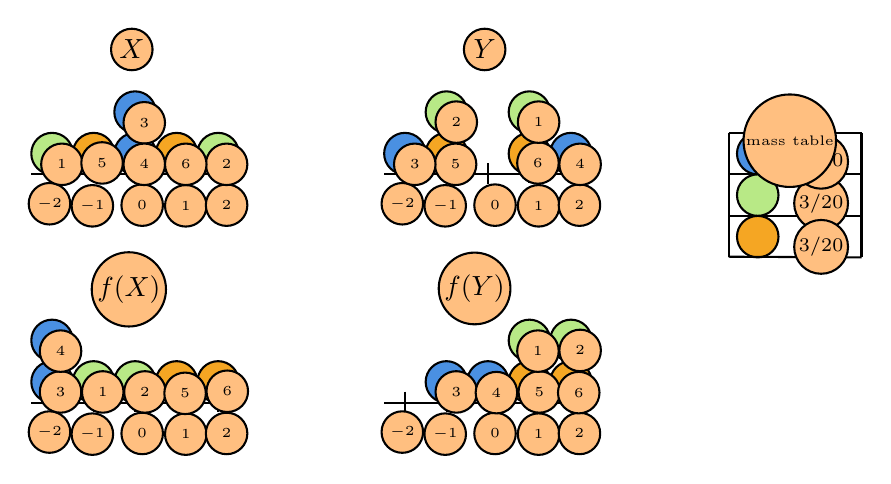
\begin{tikzpicture}[x=0.75pt,y=0.75pt,yscale=-1,xscale=1]
		%uncomment if require: \path (0,300); %set diagram left start at 0, and has height of 300
		
		%Straight Lines [id:da35193445462267636] 
		\draw    (80,130) -- (180,130) ;
		%Straight Lines [id:da9807637694958036] 
		\draw    (130,124.67) -- (130,134.67) ;
		%Straight Lines [id:da46079474054289493] 
		\draw    (110.33,124.33) -- (110.33,134.33) ;
		%Straight Lines [id:da9266328965717958] 
		\draw    (90,124.67) -- (90,134.67) ;
		%Straight Lines [id:da26812861847968716] 
		\draw    (150,124) -- (150,134) ;
		%Straight Lines [id:da21560973066226619] 
		\draw    (170,124.33) -- (170,134.33) ;
		%Shape: Circle [id:dp6385632921074851] 
		\draw  [fill={rgb, 255:red, 184; green, 233; blue, 134 }  ,fill opacity=1 ] (80,120) .. controls (80,114.48) and (84.48,110) .. (90,110) .. controls (95.52,110) and (100,114.48) .. (100,120) .. controls (100,125.52) and (95.52,130) .. (90,130) .. controls (84.48,130) and (80,125.52) .. (80,120) -- cycle ;
		%Shape: Circle [id:dp88757539189809] 
		\draw  [fill={rgb, 255:red, 184; green, 233; blue, 134 }  ,fill opacity=1 ] (160,120) .. controls (160,114.48) and (164.48,110) .. (170,110) .. controls (175.52,110) and (180,114.48) .. (180,120) .. controls (180,125.52) and (175.52,130) .. (170,130) .. controls (164.48,130) and (160,125.52) .. (160,120) -- cycle ;
		%Shape: Circle [id:dp00023416890886918118] 
		\draw  [fill={rgb, 255:red, 74; green, 144; blue, 226 }  ,fill opacity=1 ] (120,120) .. controls (120,114.48) and (124.48,110) .. (130,110) .. controls (135.52,110) and (140,114.48) .. (140,120) .. controls (140,125.52) and (135.52,130) .. (130,130) .. controls (124.48,130) and (120,125.52) .. (120,120) -- cycle ;
		%Shape: Circle [id:dp5305226281914701] 
		\draw  [fill={rgb, 255:red, 74; green, 144; blue, 226 }  ,fill opacity=1 ] (120,100) .. controls (120,94.48) and (124.48,90) .. (130,90) .. controls (135.52,90) and (140,94.48) .. (140,100) .. controls (140,105.52) and (135.52,110) .. (130,110) .. controls (124.48,110) and (120,105.52) .. (120,100) -- cycle ;
		%Shape: Circle [id:dp8678638550856308] 
		\draw  [fill={rgb, 255:red, 245; green, 166; blue, 35 }  ,fill opacity=1 ] (100,120) .. controls (100,114.48) and (104.48,110) .. (110,110) .. controls (115.52,110) and (120,114.48) .. (120,120) .. controls (120,125.52) and (115.52,130) .. (110,130) .. controls (104.48,130) and (100,125.52) .. (100,120) -- cycle ;
		%Shape: Circle [id:dp3017884596296905] 
		\draw  [fill={rgb, 255:red, 245; green, 166; blue, 35 }  ,fill opacity=1 ] (140,120) .. controls (140,114.48) and (144.48,110) .. (150,110) .. controls (155.52,110) and (160,114.48) .. (160,120) .. controls (160,125.52) and (155.52,130) .. (150,130) .. controls (144.48,130) and (140,125.52) .. (140,120) -- cycle ;
		%Straight Lines [id:da0560420025775803] 
		\draw    (250,130) -- (350,130) ;
		%Straight Lines [id:da2151747914618083] 
		\draw    (300,124.67) -- (300,134.67) ;
		%Straight Lines [id:da5495384586463741] 
		\draw    (280.33,124.33) -- (280.33,134.33) ;
		%Straight Lines [id:da7015652694438574] 
		\draw    (260,124.67) -- (260,134.67) ;
		%Straight Lines [id:da5295885469027419] 
		\draw    (320,124) -- (320,134) ;
		%Straight Lines [id:da5874340098395976] 
		\draw    (340,124.33) -- (340,134.33) ;
		%Shape: Circle [id:dp6241858667847562] 
		\draw  [fill={rgb, 255:red, 184; green, 233; blue, 134 }  ,fill opacity=1 ] (270,100) .. controls (270,94.48) and (274.48,90) .. (280,90) .. controls (285.52,90) and (290,94.48) .. (290,100) .. controls (290,105.52) and (285.52,110) .. (280,110) .. controls (274.48,110) and (270,105.52) .. (270,100) -- cycle ;
		%Shape: Circle [id:dp5883247401593619] 
		\draw  [fill={rgb, 255:red, 184; green, 233; blue, 134 }  ,fill opacity=1 ] (310,100) .. controls (310,94.48) and (314.48,90) .. (320,90) .. controls (325.52,90) and (330,94.48) .. (330,100) .. controls (330,105.52) and (325.52,110) .. (320,110) .. controls (314.48,110) and (310,105.52) .. (310,100) -- cycle ;
		%Shape: Circle [id:dp7734578621303227] 
		\draw  [fill={rgb, 255:red, 74; green, 144; blue, 226 }  ,fill opacity=1 ] (330,120) .. controls (330,114.48) and (334.48,110) .. (340,110) .. controls (345.52,110) and (350,114.48) .. (350,120) .. controls (350,125.52) and (345.52,130) .. (340,130) .. controls (334.48,130) and (330,125.52) .. (330,120) -- cycle ;
		%Shape: Circle [id:dp8014577169403472] 
		\draw  [fill={rgb, 255:red, 74; green, 144; blue, 226 }  ,fill opacity=1 ] (250,120) .. controls (250,114.48) and (254.48,110) .. (260,110) .. controls (265.52,110) and (270,114.48) .. (270,120) .. controls (270,125.52) and (265.52,130) .. (260,130) .. controls (254.48,130) and (250,125.52) .. (250,120) -- cycle ;
		%Shape: Circle [id:dp7009708547845324] 
		\draw  [fill={rgb, 255:red, 245; green, 166; blue, 35 }  ,fill opacity=1 ] (270,120) .. controls (270,114.48) and (274.48,110) .. (280,110) .. controls (285.52,110) and (290,114.48) .. (290,120) .. controls (290,125.52) and (285.52,130) .. (280,130) .. controls (274.48,130) and (270,125.52) .. (270,120) -- cycle ;
		%Shape: Circle [id:dp17515543966196323] 
		\draw  [fill={rgb, 255:red, 245; green, 166; blue, 35 }  ,fill opacity=1 ] (310,120) .. controls (310,114.48) and (314.48,110) .. (320,110) .. controls (325.52,110) and (330,114.48) .. (330,120) .. controls (330,125.52) and (325.52,130) .. (320,130) .. controls (314.48,130) and (310,125.52) .. (310,120) -- cycle ;
		%Straight Lines [id:da047683271260472004] 
		\draw    (80,240) -- (180,240) ;
		%Straight Lines [id:da06897596646315929] 
		\draw    (130,234.67) -- (130,244.67) ;
		%Straight Lines [id:da6001225133609294] 
		\draw    (110.33,234.33) -- (110.33,244.33) ;
		%Straight Lines [id:da7759787210653073] 
		\draw    (90,234.67) -- (90,244.67) ;
		%Straight Lines [id:da4808256794065102] 
		\draw    (150,234) -- (150,244) ;
		%Straight Lines [id:da15879435329235903] 
		\draw    (170,234.33) -- (170,244.33) ;
		%Shape: Circle [id:dp28723372250138723] 
		\draw  [fill={rgb, 255:red, 184; green, 233; blue, 134 }  ,fill opacity=1 ] (120,230) .. controls (120,224.48) and (124.48,220) .. (130,220) .. controls (135.52,220) and (140,224.48) .. (140,230) .. controls (140,235.52) and (135.52,240) .. (130,240) .. controls (124.48,240) and (120,235.52) .. (120,230) -- cycle ;
		%Shape: Circle [id:dp48538304745438854] 
		\draw  [fill={rgb, 255:red, 184; green, 233; blue, 134 }  ,fill opacity=1 ] (100,230) .. controls (100,224.48) and (104.48,220) .. (110,220) .. controls (115.52,220) and (120,224.48) .. (120,230) .. controls (120,235.52) and (115.52,240) .. (110,240) .. controls (104.48,240) and (100,235.52) .. (100,230) -- cycle ;
		%Shape: Circle [id:dp29386895845676997] 
		\draw  [fill={rgb, 255:red, 74; green, 144; blue, 226 }  ,fill opacity=1 ] (80,210) .. controls (80,204.48) and (84.48,200) .. (90,200) .. controls (95.52,200) and (100,204.48) .. (100,210) .. controls (100,215.52) and (95.52,220) .. (90,220) .. controls (84.48,220) and (80,215.52) .. (80,210) -- cycle ;
		%Shape: Circle [id:dp5371834929031682] 
		\draw  [fill={rgb, 255:red, 74; green, 144; blue, 226 }  ,fill opacity=1 ] (80,230) .. controls (80,224.48) and (84.48,220) .. (90,220) .. controls (95.52,220) and (100,224.48) .. (100,230) .. controls (100,235.52) and (95.52,240) .. (90,240) .. controls (84.48,240) and (80,235.52) .. (80,230) -- cycle ;
		%Shape: Circle [id:dp679780772291168] 
		\draw  [fill={rgb, 255:red, 245; green, 166; blue, 35 }  ,fill opacity=1 ] (160,230) .. controls (160,224.48) and (164.48,220) .. (170,220) .. controls (175.52,220) and (180,224.48) .. (180,230) .. controls (180,235.52) and (175.52,240) .. (170,240) .. controls (164.48,240) and (160,235.52) .. (160,230) -- cycle ;
		%Shape: Circle [id:dp09916225023407454] 
		\draw  [fill={rgb, 255:red, 245; green, 166; blue, 35 }  ,fill opacity=1 ] (140,230) .. controls (140,224.48) and (144.48,220) .. (150,220) .. controls (155.52,220) and (160,224.48) .. (160,230) .. controls (160,235.52) and (155.52,240) .. (150,240) .. controls (144.48,240) and (140,235.52) .. (140,230) -- cycle ;
		%Straight Lines [id:da005830372732677835] 
		\draw    (250,240) -- (350,240) ;
		%Straight Lines [id:da8496538110163001] 
		\draw    (300,234.67) -- (300,244.67) ;
		%Straight Lines [id:da5296637264047355] 
		\draw    (280.33,234.33) -- (280.33,244.33) ;
		%Straight Lines [id:da5680895817724656] 
		\draw    (260,234.67) -- (260,244.67) ;
		%Straight Lines [id:da07030570834807603] 
		\draw    (320,234) -- (320,244) ;
		%Straight Lines [id:da9703804817895982] 
		\draw    (340,234.33) -- (340,244.33) ;
		%Shape: Circle [id:dp5027333987636868] 
		\draw  [fill={rgb, 255:red, 184; green, 233; blue, 134 }  ,fill opacity=1 ] (330,210) .. controls (330,204.48) and (334.48,200) .. (340,200) .. controls (345.52,200) and (350,204.48) .. (350,210) .. controls (350,215.52) and (345.52,220) .. (340,220) .. controls (334.48,220) and (330,215.52) .. (330,210) -- cycle ;
		%Shape: Circle [id:dp4629972047973214] 
		\draw  [fill={rgb, 255:red, 184; green, 233; blue, 134 }  ,fill opacity=1 ] (310,210) .. controls (310,204.48) and (314.48,200) .. (320,200) .. controls (325.52,200) and (330,204.48) .. (330,210) .. controls (330,215.52) and (325.52,220) .. (320,220) .. controls (314.48,220) and (310,215.52) .. (310,210) -- cycle ;
		%Shape: Circle [id:dp7126456798766247] 
		\draw  [fill={rgb, 255:red, 74; green, 144; blue, 226 }  ,fill opacity=1 ] (290,230) .. controls (290,224.48) and (294.48,220) .. (300,220) .. controls (305.52,220) and (310,224.48) .. (310,230) .. controls (310,235.52) and (305.52,240) .. (300,240) .. controls (294.48,240) and (290,235.52) .. (290,230) -- cycle ;
		%Shape: Circle [id:dp702252322428877] 
		\draw  [fill={rgb, 255:red, 74; green, 144; blue, 226 }  ,fill opacity=1 ] (270,230) .. controls (270,224.48) and (274.48,220) .. (280,220) .. controls (285.52,220) and (290,224.48) .. (290,230) .. controls (290,235.52) and (285.52,240) .. (280,240) .. controls (274.48,240) and (270,235.52) .. (270,230) -- cycle ;
		%Shape: Circle [id:dp7540659628053352] 
		\draw  [fill={rgb, 255:red, 245; green, 166; blue, 35 }  ,fill opacity=1 ] (330,230) .. controls (330,224.48) and (334.48,220) .. (340,220) .. controls (345.52,220) and (350,224.48) .. (350,230) .. controls (350,235.52) and (345.52,240) .. (340,240) .. controls (334.48,240) and (330,235.52) .. (330,230) -- cycle ;
		%Shape: Circle [id:dp6870485382076588] 
		\draw  [fill={rgb, 255:red, 245; green, 166; blue, 35 }  ,fill opacity=1 ] (310,230) .. controls (310,224.48) and (314.48,220) .. (320,220) .. controls (325.52,220) and (330,224.48) .. (330,230) .. controls (330,235.52) and (325.52,240) .. (320,240) .. controls (314.48,240) and (310,235.52) .. (310,230) -- cycle ;
		%Shape: Circle [id:dp5522689388859041] 
		\draw  [fill={rgb, 255:red, 74; green, 144; blue, 226 }  ,fill opacity=1 ] (420,120) .. controls (420,114.48) and (424.48,110) .. (430,110) .. controls (435.52,110) and (440,114.48) .. (440,120) .. controls (440,125.52) and (435.52,130) .. (430,130) .. controls (424.48,130) and (420,125.52) .. (420,120) -- cycle ;
		%Shape: Circle [id:dp6539414929940437] 
		\draw  [fill={rgb, 255:red, 184; green, 233; blue, 134 }  ,fill opacity=1 ] (420,140) .. controls (420,134.48) and (424.48,130) .. (430,130) .. controls (435.52,130) and (440,134.48) .. (440,140) .. controls (440,145.52) and (435.52,150) .. (430,150) .. controls (424.48,150) and (420,145.52) .. (420,140) -- cycle ;
		%Shape: Circle [id:dp010055052010330856] 
		\draw  [fill={rgb, 255:red, 245; green, 166; blue, 35 }  ,fill opacity=1 ] (420,160) .. controls (420,154.48) and (424.48,150) .. (430,150) .. controls (435.52,150) and (440,154.48) .. (440,160) .. controls (440,165.52) and (435.52,170) .. (430,170) .. controls (424.48,170) and (420,165.52) .. (420,160) -- cycle ;
		%Straight Lines [id:da40237805847461217] 
		\draw    (416,110) -- (480,110) ;
		%Straight Lines [id:da7413023184354017] 
		\draw    (416,169.67) -- (480,170) ;
		%Straight Lines [id:da9392849789444075] 
		\draw    (416,110) -- (416,169.67) ;
		%Straight Lines [id:da8876656319892611] 
		\draw    (480,110) -- (480,170) ;
		%Straight Lines [id:da7468150014903507] 
		\draw    (416,130) -- (480,130) ;
		%Straight Lines [id:da07186517033445994] 
		\draw    (416,150) -- (480,150) ;
		
		% Text Node
		\draw (126,137.4) node [anchor=north west][inner sep=0.75pt]  [font=\tiny]  {$0$};
		% Text Node
		\draw (147,137.73) node [anchor=north west][inner sep=0.75pt]  [font=\tiny]  {$1$};
		% Text Node
		\draw (166.67,137.4) node [anchor=north west][inner sep=0.75pt]  [font=\tiny]  {$2$};
		% Text Node
		\draw (81.33,136.73) node [anchor=north west][inner sep=0.75pt]  [font=\tiny]  {$-2$};
		% Text Node
		\draw (102,137.73) node [anchor=north west][inner sep=0.75pt]  [font=\tiny]  {$-1$};
		% Text Node
		\draw (296,137.4) node [anchor=north west][inner sep=0.75pt]  [font=\tiny]  {$0$};
		% Text Node
		\draw (317,137.73) node [anchor=north west][inner sep=0.75pt]  [font=\tiny]  {$1$};
		% Text Node
		\draw (336.67,137.4) node [anchor=north west][inner sep=0.75pt]  [font=\tiny]  {$2$};
		% Text Node
		\draw (251.33,136.73) node [anchor=north west][inner sep=0.75pt]  [font=\tiny]  {$-2$};
		% Text Node
		\draw (272,137.73) node [anchor=north west][inner sep=0.75pt]  [font=\tiny]  {$-1$};
		% Text Node
		\draw (126,247.4) node [anchor=north west][inner sep=0.75pt]  [font=\tiny]  {$0$};
		% Text Node
		\draw (147,247.73) node [anchor=north west][inner sep=0.75pt]  [font=\tiny]  {$1$};
		% Text Node
		\draw (166.67,247.4) node [anchor=north west][inner sep=0.75pt]  [font=\tiny]  {$2$};
		% Text Node
		\draw (81.33,246.73) node [anchor=north west][inner sep=0.75pt]  [font=\tiny]  {$-2$};
		% Text Node
		\draw (102,247.73) node [anchor=north west][inner sep=0.75pt]  [font=\tiny]  {$-1$};
		% Text Node
		\draw (296,247.4) node [anchor=north west][inner sep=0.75pt]  [font=\tiny]  {$0$};
		% Text Node
		\draw (317,247.73) node [anchor=north west][inner sep=0.75pt]  [font=\tiny]  {$1$};
		% Text Node
		\draw (336.67,247.4) node [anchor=north west][inner sep=0.75pt]  [font=\tiny]  {$2$};
		% Text Node
		\draw (251.33,246.73) node [anchor=north west][inner sep=0.75pt]  [font=\tiny]  {$-2$};
		% Text Node
		\draw (272,247.73) node [anchor=north west][inner sep=0.75pt]  [font=\tiny]  {$-1$};
		% Text Node
		\draw (121,62.4) node [anchor=north west][inner sep=0.75pt]    {$X$};
		% Text Node
		\draw (291,62.4) node [anchor=north west][inner sep=0.75pt]    {$Y$};
		% Text Node
		\draw (114,172.4) node [anchor=north west][inner sep=0.75pt]    {$f( X)$};
		% Text Node
		\draw (281,172.4) node [anchor=north west][inner sep=0.75pt]    {$f( Y)$};
		% Text Node
		\draw (451,134.4) node [anchor=north west][inner sep=0.75pt]  [font=\scriptsize]  {$3/20$};
		% Text Node
		\draw (451,114.4) node [anchor=north west][inner sep=0.75pt]  [font=\scriptsize]  {$4/20$};
		% Text Node
		\draw (451,155.4) node [anchor=north west][inner sep=0.75pt]  [font=\scriptsize]  {$3/20$};
		% Text Node
		\draw (429.33,97.67) node [anchor=north west][inner sep=0.75pt]  [font=\tiny] [align=left] {mass table};
		% Text Node
		\draw (87.33,117.73) node [anchor=north west][inner sep=0.75pt]  [font=\tiny]  {$1$};
		% Text Node
		\draw (166.67,117.73) node [anchor=north west][inner sep=0.75pt]  [font=\tiny]  {$2$};
		% Text Node
		\draw (127,97.73) node [anchor=north west][inner sep=0.75pt]  [font=\tiny]  {$3$};
		% Text Node
		\draw (127,117.73) node [anchor=north west][inner sep=0.75pt]  [font=\tiny]  {$4$};
		% Text Node
		\draw (106.67,117.07) node [anchor=north west][inner sep=0.75pt]  [font=\tiny]  {$5$};
		% Text Node
		\draw (147,117.73) node [anchor=north west][inner sep=0.75pt]  [font=\tiny]  {$6$};
		% Text Node
		\draw (277,117.73) node [anchor=north west][inner sep=0.75pt]  [font=\tiny]  {$5$};
		% Text Node
		\draw (316.67,117.07) node [anchor=north west][inner sep=0.75pt]  [font=\tiny]  {$6$};
		% Text Node
		\draw (257.33,117.73) node [anchor=north west][inner sep=0.75pt]  [font=\tiny]  {$3$};
		% Text Node
		\draw (277.33,97.4) node [anchor=north west][inner sep=0.75pt]  [font=\tiny]  {$2$};
		% Text Node
		\draw (317,97.4) node [anchor=north west][inner sep=0.75pt]  [font=\tiny]  {$1$};
		% Text Node
		\draw (337,117.73) node [anchor=north west][inner sep=0.75pt]  [font=\tiny]  {$4$};
		% Text Node
		\draw (107,227.4) node [anchor=north west][inner sep=0.75pt]  [font=\tiny]  {$1$};
		% Text Node
		\draw (127.33,227.4) node [anchor=north west][inner sep=0.75pt]  [font=\tiny]  {$2$};
		% Text Node
		\draw (146.67,228.07) node [anchor=north west][inner sep=0.75pt]  [font=\tiny]  {$5$};
		% Text Node
		\draw (167,227.07) node [anchor=north west][inner sep=0.75pt]  [font=\tiny]  {$6$};
		% Text Node
		\draw (86.67,227.4) node [anchor=north west][inner sep=0.75pt]  [font=\tiny]  {$3$};
		% Text Node
		\draw (86.67,207.73) node [anchor=north west][inner sep=0.75pt]  [font=\tiny]  {$4$};
		% Text Node
		\draw (277.33,227.4) node [anchor=north west][inner sep=0.75pt]  [font=\tiny]  {$3$};
		% Text Node
		\draw (296.67,227.73) node [anchor=north west][inner sep=0.75pt]  [font=\tiny]  {$4$};
		% Text Node
		\draw (317.33,227.4) node [anchor=north west][inner sep=0.75pt]  [font=\tiny]  {$5$};
		% Text Node
		\draw (336.33,227.73) node [anchor=north west][inner sep=0.75pt]  [font=\tiny]  {$6$};
		% Text Node
		\draw (316.67,207.73) node [anchor=north west][inner sep=0.75pt]  [font=\tiny]  {$1$};
		% Text Node
		\draw (337,207.4) node [anchor=north west][inner sep=0.75pt]  [font=\tiny]  {$2$};
		
		
	\end{tikzpicture}
\end{figure}
	 Note that we can also find other Borel measurable function. For instance you can figure out a continuous function that behaves differently on positive numbers, vs. negative numbers.
\end{solution}

\begin{problem}
	Prove that if $ \set{Z_n} $ converges to $ X $ almost surely, then for each $ \epsilon>0 $ we have $ \prob(\abs{Z_n - Z}\geq \epsilon\ i.o.) = 0 $.
\end{problem}
\begin{solution}
	We start with
	\begin{align*}
		1 = \prob(Z_n\to Z) &= \prob(\bigcap_{q\in\Q^+}\set{\abs{Z_n-Z}<q\ a.a.}) \\
		&= 1 - \prob(\bigcup_{q\in\Q^+}\set{\abs{Z_n-Z}\geqq\ i.o.})
	\end{align*}
	Thus
	\[ \prob(\bigcup_{q\in\Q^+}\set{\abs{Z_n-Z}\geq\ i.o.}) = 0. \]
	Observe that for all $ \epsilon>0 $
	\[ \set{\abs{Z_n-Z}\geq\epsilon\ i.o.} \subseteq \bigcup_{q\in\Q}\set{\abs{Z_n-Z}\geq q\ i.o.}. \]
	Thus by monotonicity of the probability function we will have
	\[ \prob(\set{\abs{Z_n-Z}\geq\epsilon\ i.o.}) \leq \prob(\bigcup_{q\in\Q}\set{\abs{Z_n-Z}\geq q\ i.o.}) = 0. \]
	So
	\[  \prob(\set{\abs{Z_n-Z}\geq\epsilon\ i.o.}) = 0. \]
\end{solution}


\begin{problem}
	Let $ X_1,X_2,\cdots $ be a sequence of random variables that are independent. Then prove that \[ X_n \to X \ a.s. \implies \sum_n \prob(\abs{X_n-X}>\epsilon) < \infty. \]
\end{problem}
\begin{solution}
	We do by the proof by contrapositive. 
	We want to proof 
	$$ \exists \epsilon>0 \quad \sum_{n} \mathbb{P}(|X_n-X|>\epsilon) = \infty \implies P(X_n\to X) = 0 $$
	
	Since $X_n$'s are independent, then by Borel-Cantelli we have
	\[ \mathbb{P}(|X_n-X|>\epsilon\ i.o.) = 1. \tag{1}. \]
	This implies 
	\[ \mathbb{P}(\bigcup_{q\in \mathbb{Q}^+} \{|X_n-X|>q\ i.o.\}) = 1. \tag{2} \]
	(if this is not clear for you see the remark below)
	
	Thus
	$$ \mathbb{P}(\bigcap_{r\in\mathbb{Q}^+}\{|X_n-X|\leq q\ a.a.\}) = 0. $$
	
	which is equivalent to 
	$$ \mathbb{P}(X_n \to X) = 0. \qed $$
\end{solution}
\begin{remark}
	To see why (1) implies (2) see the below:
	$$\{|X_n-X|>\epsilon\ i.o.\} \subseteq \bigcup_{q\in \mathbb{Q}} \{|X_n-X|>q\ i.o.\}.$$
	By monotonicity of the probability measure
	$$ 1 = \mathbb{P}(\{|X_n-X|>\epsilon\ i.o.\}) \leq \mathbb{P}(\bigcup_{q\in \mathbb{Q}^+} \{|X_n-X|>q\ i.o.\}).$$
	Thus 
	$$ \mathbb{P}(\bigcup_{q\in \mathbb{Q}^+} \{|X_n-X|>q\ i.o.\}) = 1. $$
\end{remark}

\begin{problem}
	Let $ X_1,X_2,\cdots $ be a sequence of independent random variable with $ \prob(X_n=3^n) = \prob(X_n = 3^{-n}) = \frac{1}{2} $. Let $ S_n = X_1+\cdots+X_n $.
	\begin{enumerate}[(a)]
		\item Compute $ \E{X_n} $ for each $ n $.
		\item For $ n \in \N $, compute $ R_n $ defined as
		\[ R_n = \sup\set{r\in\R : \prob(\abs{S_n}\geq r) = 1}, \]
		i.e. the largest number such that $ \abs{S_n} $ is always at least $ R_n $.
		\item Compute $ \lim_{n\to\infty}R_n/n $.
		\item For which $ \epsilon>0 $ (if any) is it the case that $ \prob(\frac{1}{n}\abs{S_n}\geq \epsilon)\not\to 0? $
		\item Why does this result not contradict the various laws of large numbers?
	\end{enumerate}
\end{problem}
\begin{solution}
	\begin{enumerate}[(a)]
		\item Observe that $ X_n $ is a simple random variable, thus
		\[ \E{X_n} = \frac{1}{2}3^n - \frac{1}{2}3^{n} = 0. \]
		
		\item The value of $ R_n $ equal to the case where for $ S_n $ all the random variables $ X_1,X_2,\cdots, X_{n-1} $ assume their lowest value i.e. $ -3,-9,\cdots,-3^{n-1} $ respectively, and the random variable $ X_n $ assumes its largest value, i.e. $ 3^n $.
		So we will have
		\[ S_n = 3^n - (3+9+\cdots+3^{n-1}) = 3^n - \frac{3^n-3}{2} = \frac{3^n+3}{2}. \]
		
		\item From what we had in part (b) we can see that
		\[ \lim_{n\to\infty}\frac{R_n}{n} = \lim_{n\to\infty}\frac{3^n + 3}{2n} = \infty. \]
		
		\item There is no $ \epsilon>0 $ that works. That is because we know that $ \abs{S_n} \geq R_n $ almost everywhere. On the other hand, in part (b) we observed that $ R_n/n \to \infty$ as $ n\to\infty $. So for all $ \epsilon>0 $ the sequence of reals $ \prob(\abs{S_n}/n\geq \epsilon) $ will converge to zero.
		
		\item This does not contradicts any of the law of large number. That is because the variance of $ X_n $ is
		\[ \Var(X_n) = \E{X^2} - \E{X}^2 = 3^n, \]
		which does not remain finite as $ n\to\infty $.
	\end{enumerate}
\end{solution}

\begin{problem}
	Suppose $ \E{2^X}=4 $. Prove that $ \prob(X\geq 3)\leq 1/2 $.
\end{problem}
\begin{solution}[The first method]
	We can start with
	\[ \E{2^X} = \E{2^X\mathds{1}_{X\geq3}} + \E{2^X\mathds{1}_{X<3}} = 4. \]
	For the first and the second terms we have the following bounds
	\[ \E{2^X\mathds{1}_{X\geq3}} \geq 8\prob(X\geq 3), \]
	So 
	\[ 8\prob(X\geq 3) \leq \E{2^X\mathds{1}_{X\geq 3}} = 4 - \E{2^X\mathds{1}_{X<3}}. \]
	This implies that 
	\[ \prob(X\geq 3) \leq \frac{1}{2} - \E{2^X\mathds{1}_{X<3}} \leq \frac{1}{2}, \]
	where we have used the fact that the expectation of a non-negative random variable is positive.
\end{solution}
\begin{remark}[Connection to the conditional expectation]
	If one has already used the conditional expectation before, then they can recover the definition of it using the answer above. 
	\[ \E{X\mathds{1}_B} = \E{X|B} \E{\mathds{1}_B} = \E{X|B}\prob(B).  \]
	In fact the conditional expectation is a way to factor the expectation when the random variable is of the form $ X\mathds{1}_A $.
\end{remark}
\begin{solution}[The second method]
	Define the random variable
	\[ Y = 2^X. \]
	Thus $ X = \log(Y) $, where $ \log $ is considered to be base 2 logarithm function. Thus
	\[ \prob(X\geq 3) = \prob(\log(Y)\geq 3) = \prob(Y\geq 9) \leq \frac{\E{Y}}{9} \frac{4}{9}\leq \frac{4}{8} = \frac{1}{2}, \]
	where we have used the Markov's inequality. Note that the random variable $ Y $ is non-negative and that is the reason we could use the Markov's inequality.
\end{solution}

\begin{problem}
	Give examples of random variables $ Y $ with mean $ 0 $ and variance $ 1 $ such that
	\begin{enumerate}[(a)]
		\item $ \prob(\abs{Y}\geq 2) = 1/4 $.
		\item $ \prob(\abs{Y}\geq 2) < 1/4 $.
	\end{enumerate}
\end{problem}
\begin{solution}
	For all of the examples below let $ ([0,1],\mathbb{B},\lambda) $ be the probability space.
	\begin{enumerate}[(a)]
		\item An easy example is
		\[ X = 2\mathds{1}_{[0,1/8)} -2\mathds{1}_{(1/8,2/8]}. \]
		The graph of this random variable would look like as the following.
		\begin{figure}[h!]
	\centering
	
	
	
	\tikzset{every picture/.style={line width=0.75pt}} %set default line width to 0.75pt        
	
	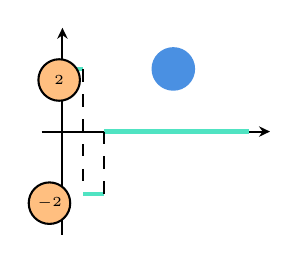
\begin{tikzpicture}[x=0.75pt,y=0.75pt,yscale=-1,xscale=1]
		%uncomment if require: \path (0,300); %set diagram left start at 0, and has height of 300
		
		%Straight Lines [id:da6563983846558457] 
		\draw    (120,130) -- (227,130) ;
		\draw [shift={(230,130)}, rotate = 180] [fill={rgb, 255:red, 0; green, 0; blue, 0 }  ][line width=0.08]  [draw opacity=0] (5.36,-2.57) -- (0,0) -- (5.36,2.57) -- (3.56,0) -- cycle    ;
		%Straight Lines [id:da6113625186161247] 
		\draw    (130,83) -- (130,180) ;
		\draw [shift={(130,80)}, rotate = 90] [fill={rgb, 255:red, 0; green, 0; blue, 0 }  ][line width=0.08]  [draw opacity=0] (5.36,-2.57) -- (0,0) -- (5.36,2.57) -- (3.56,0) -- cycle    ;
		%Straight Lines [id:da18823649577209234] 
		\draw [color={rgb, 255:red, 80; green, 227; blue, 194 }  ,draw opacity=1 ][line width=1.5]    (130,100) -- (140,100) ;
		%Straight Lines [id:da23901203978356844] 
		\draw [color={rgb, 255:red, 80; green, 227; blue, 194 }  ,draw opacity=1 ][line width=1.5]    (140,160) -- (150,160) ;
		%Straight Lines [id:da7372403791207396] 
		\draw [color={rgb, 255:red, 80; green, 227; blue, 194 }  ,draw opacity=1 ][line width=1.5]    (150,130) -- (220,130) ;
		%Straight Lines [id:da23626914265612498] 
		\draw  [dash pattern={on 4.5pt off 4.5pt}]  (140,100) -- (140,160) ;
		%Straight Lines [id:da051763154265799693] 
		\draw  [dash pattern={on 4.5pt off 4.5pt}]  (150,130) -- (150,160) ;
		
		% Text Node
		\draw (121,97.73) node [anchor=north west][inner sep=0.75pt]  [font=\tiny]  {$2$};
		% Text Node
		\draw (116.33,157.07) node [anchor=north west][inner sep=0.75pt]  [font=\tiny]  {$-2$};
		% Text Node
		\draw (176,92.4) node [anchor=north west][inner sep=0.75pt]  [color={rgb, 255:red, 74; green, 144; blue, 226 }  ,opacity=1 ]  {$Y$};
		
		
	\end{tikzpicture}
\end{figure}
		\FloatBarrier
		\item The following example is a straightforward one.
		\[ X = 2\mathds{1}_{[0,1/16)} - 2\mathds{1}_{[1/16,2/16)} + \mathds{1}_{(2/16,6/16]} - \mathds{1}_{(6/16,10/16]}. \]
		\begin{figure}[h!]
	\centering
	
	
	
	\tikzset{every picture/.style={line width=0.75pt}} %set default line width to 0.75pt        
	
	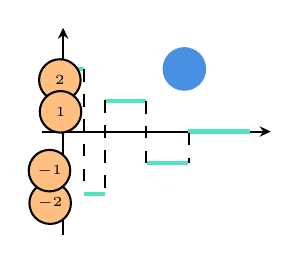
\begin{tikzpicture}[x=0.75pt,y=0.75pt,yscale=-1,xscale=1]
		%uncomment if require: \path (0,300); %set diagram left start at 0, and has height of 300
		
		%Straight Lines [id:da6563983846558457] 
		\draw    (120,130) -- (227,130) ;
		\draw [shift={(230,130)}, rotate = 180] [fill={rgb, 255:red, 0; green, 0; blue, 0 }  ][line width=0.08]  [draw opacity=0] (5.36,-2.57) -- (0,0) -- (5.36,2.57) -- (3.56,0) -- cycle    ;
		%Straight Lines [id:da6113625186161247] 
		\draw    (130,83) -- (130,180) ;
		\draw [shift={(130,80)}, rotate = 90] [fill={rgb, 255:red, 0; green, 0; blue, 0 }  ][line width=0.08]  [draw opacity=0] (5.36,-2.57) -- (0,0) -- (5.36,2.57) -- (3.56,0) -- cycle    ;
		%Straight Lines [id:da18823649577209234] 
		\draw [color={rgb, 255:red, 80; green, 227; blue, 194 }  ,draw opacity=1 ][line width=1.5]    (130,100) -- (140,100) ;
		%Straight Lines [id:da23901203978356844] 
		\draw [color={rgb, 255:red, 80; green, 227; blue, 194 }  ,draw opacity=1 ][line width=1.5]    (140,160) -- (150,160) ;
		%Straight Lines [id:da7372403791207396] 
		\draw [color={rgb, 255:red, 80; green, 227; blue, 194 }  ,draw opacity=1 ][line width=1.5]    (190,130) -- (220,130) ;
		%Straight Lines [id:da28780295701567704] 
		\draw [color={rgb, 255:red, 80; green, 227; blue, 194 }  ,draw opacity=1 ][line width=1.5]    (150,115.33) -- (170,115.33) ;
		%Straight Lines [id:da5129439211809914] 
		\draw [color={rgb, 255:red, 80; green, 227; blue, 194 }  ,draw opacity=1 ][line width=1.5]    (170.33,145) -- (190.33,145) ;
		%Straight Lines [id:da8570092074976612] 
		\draw  [dash pattern={on 4.5pt off 4.5pt}]  (140,100) -- (140,160) ;
		%Straight Lines [id:da9540488747278426] 
		\draw  [dash pattern={on 4.5pt off 4.5pt}]  (150.33,115) -- (150.33,160) ;
		%Straight Lines [id:da348777045876534] 
		\draw  [dash pattern={on 4.5pt off 4.5pt}]  (170,115.33) -- (170,146) ;
		%Straight Lines [id:da8594121119107911] 
		\draw  [dash pattern={on 4.5pt off 4.5pt}]  (190.67,130.67) -- (190.67,145) ;
		
		% Text Node
		\draw (121,97.73) node [anchor=north west][inner sep=0.75pt]  [font=\tiny]  {$2$};
		% Text Node
		\draw (116.33,157.07) node [anchor=north west][inner sep=0.75pt]  [font=\tiny]  {$-2$};
		% Text Node
		\draw (181,92.4) node [anchor=north west][inner sep=0.75pt]  [color={rgb, 255:red, 74; green, 144; blue, 226 }  ,opacity=1 ]  {$Y$};
		% Text Node
		\draw (121.33,113.07) node [anchor=north west][inner sep=0.75pt]  [font=\tiny]  {$1$};
		% Text Node
		\draw (116,141.4) node [anchor=north west][inner sep=0.75pt]  [font=\tiny]  {$-1$};
		
		
	\end{tikzpicture}
\end{figure}
	\end{enumerate}
\end{solution}
\begin{remark}
	Note that from the Chebychev inequality we have
	\[ \prob(\abs{Y - \mu_Y}\geq \alpha) \leq \frac{\Var(Y)}{\alpha^2}. \]
	The problem above demonstrates the cases where the equality holds, and the strict inequality holds.
\end{remark}

\begin{problem}
	Suppose $ Y $ is a random variable with finite mean $ \mu_Y $ and $ \Var(Y)=\infty $. What does Chebychev's inequality say in this case?
\end{problem}
\begin{solution}
	The Chebychev's inequality states that for any random variable $ X $ we have
	\[ \prob(\abs{X - \mu_X} \geq \alpha) \leq \frac{\Var(X)}{\alpha^2}. \]
	When $ \Var(X) = \infty $, then the Chebychev's inequality will be the trivial inequality
	\[ \prob(\abs{X - \mu_X}\geq \alpha) \leq \infty. \]
\end{solution}


\begin{problem}
	Give (with proof) an example of a sequence $ \set{Y_n} $ of jointly defined random variables, such that as $ n\to\infty $ we have all of three
	\begin{enumerate}[(i)]
		\item $ Y_n/n $ converges to $ 0 $ in probability.
		\item $ Y_n/n^2 $ converges to $ 0 $ with probability 1.
		\item $ Y_n/n $ does \emph{not} converge to 0 with probability 1.
	\end{enumerate}
\end{problem}
\begin{solution}
	Let $ ([0,1],\mathcal{B},\lambda) $ be the probability space, and define the sequence of random variables $ \set{Y_n} $ given as
	\[ Y_n = n\mathds{1}_{A_n}, \]
	where $ A_n \in \mathcal{B} $ with $ \prob(A_n) = 1/n $. Then we will have
	\[ Y_n/n = \mathds{1}_{A_n},\qquad Y_n/n^2 = \mathds{1}_{A_n}/n. \]
	Then
	\[ \prob(\abs{Y_n/n}\geq \epsilon) = 
	\begin{cases}
		0 \qquad \epsilon > 0\\
		1/n \qquad 0<\epsilon\leq 1
	\end{cases}, \qquad
	\prob(\abs{Y_n/n^2}\geq \epsilon) = 0 \qquad \text{for $ n $ large enough.}
	 \]
	 Thus we can see that $ Y_n/n $ converges to 0 in probability, $ Y_n/n $ does not converge to 0 with probability one (as $ \prob(\abs{Y_n/n}\geq \epsilon) $ is not summable). Lastly, $ Y_n/n^2 $ converges to 0 with probability 1.
\end{solution}


\begin{problem}
	Let $ r\in \N $. Let $ X_1,X_2,\cdots $ be independently distributed random variables having finite mean $ m $, which are $ r\text{-dependent} $, i.e. such that $ X_{k_1},X_{k_2},\dots,X_{k_j} $ are independent whenever $ k_{i+1}>k_i + r $ for each $ i $ (thus independent random variables are 0-dependent). Prove that with probability one $ \frac{1}{n}\sum_{i=1}^{n}X_i \to m $ as $ n\to\infty $. (\emph{Hint: break up the sum into $ r+1 $ different sums.})
\end{problem}
\begin{solution}
	Let $ S_n = \frac{1}{n}\sum_{i=1}^{n}X_i $ represent the partial sums of the infinite sum. Let $ R = r+1 $. We are interested in the subsequence terms of the form $ S_{Rn} $. These terms can be written as
	\begin{align*}
		S_{nR} &= \frac{1}{R}\cdot\frac{1}{n}(X_1+X_{1+R}+X_{1+2R}+\cdots + X_{1+(n-1)R})\\
		&+ \frac{1}{R}\cdot\frac{1}{n}(X_2+X_{2+R}+X_{2+2R}+\cdots + X_{2+(n-1)R}) \\
		&\vdots \\
		&+ \frac{1}{R}\cdot\frac{1}{n}(X_R+X_{R+R}+X_{R+2R}+\cdots + X_{R+(n-1)R}).
	\end{align*}
	Let
	\[ Y_{i,n} = \frac{1}{R}\cdot\frac{1}{n}(X_i+X_{i+R}+X_{i+2R}+\cdots + X_{i+(n-1)R}). \]
	Note that the terms in each $ Y_{i,n} $ are i.i.d. random variables by the hypothesis and all of them have mean $ n $, thus by the SLLN we have
	\[ \prob(Y_{i,n}\to m) = 1 \qquad \forall i\in \N. \]
	On the other hand, the decomposition of the sum above we can write
	\[ S_{nR} = \frac{1}{R}\sum_{i=1}^{R}Y_{{i,n}}. \]
	Each of the terms in the RHS goes to $ m $ with probability one, thus the LHS goes to $ Rm/R = m $ with probability 1.  
\end{solution}
\begin{remark}
	This is a very clear generalization of the notion of the independent random variables. In this general notion the random variables are $ r\text{-dependent} $ if they are independent whenever they are $ r $ terms away from each other. This notion will be very useful in considering the systems who have an exponentially decaying memory through time.
\end{remark}



\section{Distribution of Random Variables}

\begin{proposition}[Cumulative distribution function is right-continuous]
	Let $ X $ be a random variable whose cumulative distribution function is defined as $ F_X(x) = \prob(X \leq x) $. Then $ F_X(x) $ is right-continuous.
\end{proposition}
\begin{proof}
	Fix $ x \in \R $. Let $ \set{x_n} $ be any sequence that $ x_n \to x $ as $ n \to\infty $ and for all $ n $ $ x \leq x_n $. Observe that 
	\[ \bigcap_n (-\infty,x_n] = (-\infty,x], \tag{\eighthnote}\]
	and also 
	\[ (-\infty,x_1] \supseteq (-\infty,x_2] \supseteq (-\infty,x_3] \supseteq \cdots. \tag{\twonotes}\]
	Thus we have $ \set{(-\infty,x_n]}\downarrow (-\infty,x] $ as $ n\to\infty $. Since $ (\eighthnote) $ and $ (\twonotes) $ are both preserved by the pre-image $ \inv{X} $, so we also have
	\[ \set{\inv{X}(-\infty,x_n]}\downarrow \inv{X}((-\infty,x]) \quad \text{as $ n\to\infty $}.\]
	From continuity of probability we have
	\[ \prob(X\leq x_n) \to \prob(X\leq x) \quad \text{as } n \to \infty. \]
	Thus by the definition of cumulative distribution we have
	\[ F_X(x_n) \to F_X(x) \quad \text{as }n\to\infty. \]
\end{proof}
\begin{remark}
	Note that we can not do a similar argument to show that $ F_X(x) $ is left continuous. The obstacle is that if we choose $ \set{x_n} $ such that $ x_n\to x $ and for all $ n $ we have $ x_n \leq x $, then the union
	\[ \bigcup_n(-\infty,x_n] \]
	is not necessarily equal to $ (-\infty,x] $. For instance if we let $ x_n = x - 1/n $ then 
	\[ \bigcup_n(-\infty,x_n] = (-\infty,x). \]
\end{remark}

\begin{proposition}
	Let $ X $ and $ Y $ be two random variables (possibly defined on different probability triples). Then $ \mu_X = \mu_Y $ if and only if $ \E{f(X)} = \E{f(Y)} $ for all Borel-measurable $ f:\R \to \R $ for which either expectation is well-defined.
\end{proposition}
\begin{proof}
	To show the $ \boxed{\Longrightarrow} $, using the change of variable theorem we see that
	\[ \E{f(X)} = \int_\R f d\mu_X = \int_\R f d\mu_Y =  \E{f(Y)}. \]
	To show the $ \boxed{\Longleftarrow} $, let $ B \in \mathcal{B} $, and let $ f = \mathds{1}_B $. Then 
	\[ \E{f(X)} = \E{\mathds{1}_{B}(X)} = \E{\mathds{1}_{X\in B}} = \prob(X\in B) = \mu_X.  \]
	with a similar reasoning we get $ \E{f(Y)} = \mu_Y $. Then since $ \E{f(X)} = \E{f(Y)} $,
	\[ \mu_X = \mu_Y. \]
\end{proof}


\begin{corollary}
	If $ X $ and $ Y $ are random variables with $ \prob(X=Y) = 1 $, then \[ \E{f(X)} = \E{f(Y)} \]
	for all Borel-measurable $ f:\R \to \R $ for which either expectation is well-defined. 
\end{corollary}
\begin{proof}
	We claim that $ \prob(X=Y) = 1 $ implies $ \mu_X = \mu_Y $. To see this let $ B \in \mathcal{B} $. Then
	\begin{align*}
		\mu_X (B) = \prob(\set{X\in B}) &= \prob(\set{X\in B}\cap\set{X=Y} \dot{\cup} \set{X\in B}\cap \set{X\neq Y}) \\
		&=\prob(\set{X\in B}\cap\set{X=Y}) + \prob(\set{X\in B}\cap \set{X\neq Y})
	\end{align*}
	Note that $ \set{X\in B}\cap \set{X \neq Y} \subseteq \set{X \neq Y} $ thus from the monotonicity $ \prob(\set{X\in B}\cap \set{X \neq Y}) \leq \prob(\set{X\neq Y}) = 0 $. Thus
	\[ \mu_X (B) = \prob(\set{X\in B}) = \prob(\set{X\in B}\cap\set{X=Y}) = \prob(\set{Y\in B}\cap\set{X=Y}) = \prob(\set{Y\in B}) = \mu_Y(B). \]
	Now using the proposition above we get that
	\[ \E{f(X)} = \E{f(Y)}. \]
\end{proof}


\subsection{Solved Problems}
\begin{problem}
	Let $ \mu $ have density $ 4x^3\mathds{1}_{0<x<1} $, and let $ \nu $ have density $ x/2\mathds{1}_{0<x<2} $.
	\begin{enumerate}[(a)]
		\item Compute $ \E{X} $ where $ \mathcal{L}(X) = \mu/3 + 2\nu/3 $.
		\item Compute $ \E{Y^2} $ where $ \mathcal{L}(Y) = 1/6\mu + 1/3\delta_2 + 1/2\delta_5 $.
		\item Compute $ \E{Z^3} $ where $ \mathcal{L}(Z) = 1/8\mu+1/8\nu + 1/4\delta_3 + 1/2\delta_4 $.
	\end{enumerate}
\end{problem}

\begin{solution}
	\begin{enumerate}[(a)]
		\item Denote $ \mathcal{L}(X) $ with $ \eta $. Then by definition and then using the change of variable principle we have
		\[ \E{X} = \int_\Omega X \prob(d\omega) = \int_\R x \eta(dx) = 1/3\int_\R  x \mu(dx) + 2/3\int_\R x \nu(dx)  \]
		where for the last equality we have used the proposition 6.2.1 Rosenthal. Now using proposition 6.2.3 Rosenthal we can write
		\[ \E{X} = 4/3\int_{0}^{1} x^4 \lambda(dx)  + 1/3\int_{0}^{2} x^2 \lambda(dx)  = 4/15 + 8/9 = 52/45. \]
		where $ \lambda $ is the Lebesgue measure.
		
		\item Similar to the reasoning in part (a), we will get
		\begin{align*}
			\E{X^2} &= 1/6\int_\R x^2 \mu(dx) + 1/3\int_\R x^2 \delta_2(dx) + 1/2\int_R x^2 \delta_5(dx) \\
			&= 2/3 \int_{0}^{1}x^5 \lambda(dx) + 1/3\int_{-\infty}^{+\infty} x^2\delta(x-2)\lambda(dx) + 1/2\int_{-\infty}^{+\infty} x^2\delta(x-5)\lambda(dx) \\
			&= 2/18 + 4/3 + 25/2 = 251/18.
		\end{align*}
		
		\item Similar to the part (a) we will get
		\begin{align*}
			\E{X^3} &= 1/8\int_\R x^3 \mu(dx) + 1/8\int_\R x^3\nu(dx) + 1/4\int_\R x^3 \delta_4(dx) + 1/2\int_\R x^3\delta_4(dx) \\
			&= 1/2\int_{0}^{1}x^6\lambda(dx) + 1/16\int_{0}^{2}x^4\lambda(dx) + 1/4\int_{-\infty}^{+\infty}x^3\delta(x-3)\lambda(dx) + 1/2\int_{-\infty}^{+\infty} x^3 \delta(x-4) \lambda(dx)\\
			&=1/14 + 32/80 + 27/4 + 32.
		\end{align*}
	\end{enumerate}
\end{solution}

\begin{problem}
	Suppose $ \prob(Z=0)=\prob(Z=1)=\frac{1}{2} $, that $ Y\sim \mathcal{N}(0,1),$ and that $ Y $ and $ Z $ are independent. Set $ X=YZ $. What is the law of $ X $?
\end{problem}
\begin{solution}
	Using the conditional probability (see the proposition below), and by letting $ B\in \mathbb{B} $ we can write
	\[ \mu_X(B) = \prob(X\in B) = \prob(YZ\in B) = \prob(0\in B)\prob(Z=0) + \prob(Y\in B)\prob(Z=1) = \frac{\delta_0(B) + \mu_\mathcal{N}(B)}{2}. \]
	Thus the law of $ X $ is given by
	\[ \mu_X = \frac{\delta_0 + \mu_\mathcal{N}}{2}.\]
\end{solution}
\begin{observation}[Conditional probability and conditional expectation]
	The notion of conditional probability and conditional expectation are so natural to work with that one often forgets what is the rigorous basis of these notions. Let $ B,C \in \mathcal{F} $ be two sets that partitions the samples space $ \Omega $. Then for any $ A\in\mathcal{F} $ we can write
	\[ A =( A\cap B) \dot\cup (A \cap C).\]
	Then using the countable additivity of the probability measure we can write
	\[ \prob(A) = \prob(A\cap B) + \prob(A\cap C). \]
	We can then define the notion of the conditional probability that enables us to factor the terms in RHS in some useful sense. Define
	\[ \prob(A|B) = \prob(A\cap B)/\prob(B),\qquad \prob(A|C) = \prob(A\cap C)/\prob(C). \]
	Then we can write
	\[ \boxed{\prob(A) = \prob(A|B)\prob(B) + \prob(A|C)\prob(C).} \]
	We can do the same thing with the notion of the indicator function that is a dual notion for the set theoretic operations we had above. Again, let $ B,C $ defined as above, and let $ X $ be any random variable. Then
	\[ X = X \mathds{1}_B  + X \mathds{1}_C, \]
	where we have used the fact that 
	\[ \mathds{1}_B + \mathds{1}_C = 1 \quad \text{since } \Omega = B \dot\cup C. \]
	Then 
	\[ \E{X} = \E{X\mathds{1}_B} + \E{X\mathds{1}_C}. \]
	Now we define the notion of the conditional expectation that enables us to factor the terms in the RHS. Define
	\begin{align*}
		&\E{X|B} = \E{X\mathds{1}_B}/\E{\mathds{1}_B} = \E{X\mathds{1}_B}/\prob(B),\\ 
		&\E{X|C} = \E{X\mathds{1}_C}/\E{\mathds{1}_C} = \E{X\mathds{1}_C}/\prob(C). 
	\end{align*}
	Then we can write
	\[ \boxed{\E{X} = \E{X|B}\prob(B) + \E{X|C}\prob(C).} \]
\end{observation}

\begin{problem}
	Let $ X\sim \operatorname{Poisson}(5) $.
	\begin{enumerate}[(a)]
		\item Compute $ \E{X} $.
		\item Compute $ \Var(X) $.
		\item Compute $ \E{3^X} $. 
	\end{enumerate}
\end{problem}
\begin{solution}
	\begin{enumerate}[(a)]
		\item To find $ \E{X} $ we can start with
		\begin{align*}
			\E{X} &= \sum_{n=0}^{\infty} n \frac{e^{-\lambda} \lambda^n}{n!} \\
			&=e^{-\lambda} \sum_{n=1}^{\infty} \frac{\lambda^n}{(n-1)!} \\
			&=\lambda e^{-\lambda} \sum_{n=1}^{\infty} \frac{\lambda^{n-1}}{(n-1)!}\\
			&=\lambda e^{-\lambda} \sum_{n=0}^{\infty} \frac{\lambda^{n}}{(n)!}\\
			&=\lambda e^{-\lambda} e^\lambda \\
			&=\lambda,
		\end{align*}
		where we have used the fact that $ e^\lambda = \sum_{n=0}^{\infty}\lambda^n/n!. $
		
		\item To harvest the possible cancellations, we start with
		\begin{align*}
			\E{X(X-1)} &= \sum_{n=1}^{\infty} n(n-1) \frac{e^{-\lambda} \lambda^n}{n!} \\
			&= e^{-\lambda} \sum_{n=2}^{\infty} \frac{\lambda^n}{(n-2)!} \\
			&= \lambda^2 e^{-\lambda} \sum_{n=2}^{\infty} \frac{\lambda^{n-2}}{(n-2)!} \\
			&= \lambda^2 e^{-\lambda} \sum_{n=0}^{\infty} \frac{\lambda^{n}}{n!}\\
			&= \lambda^2 e^{-\lambda} e^\lambda \\
			&= \lambda^2.
		\end{align*}
		Thus $ \E{X(X-1)} = \E{X^2}-\E{X} = \lambda^2 $, which implies
		\[ \E{X^2} = \lambda_2 + \lambda. \]
		Now using the formula for variance we will get
		\[ \Var(X) = \E{X^2} - \E{X}^2 = \lambda^2 + \lambda - \lambda^2 = \lambda. \]
		
		
		\item We can write
		\[ \prob(3^X) = \sum_{n=0}^{\infty} 3^n \prob(X=n) = \sum_{n=0}^{\infty} 3^n \frac{e^{-\lambda}\lambda^n}{n!} = e^{-\lambda} \sum_{n=0}^{\infty} (3\lambda)^n/n! = e^{-\lambda}e^{3\lambda} = e^{2\lambda}. \]
	\end{enumerate}
\end{solution}

\begin{problem}
	Compute $ \E{X},\E{X^2} $ and ere $ \Var(X) $ where the law of $ X $ is given by
	\begin{enumerate}[(a)]
		\item $ \mathcal{L}(X) = \delta_1/2 + \lambda/2, $ where $ \lambda $ is Lebesgue measure on $ [0,1] $.
		\item $ \mathcal{L}(X) = \delta_2/3 + 2\mu_\mathcal{N}/3 $, where $ \mu_\mathcal{N} $ is the standard normal distribution $ \mathcal{N}(0,1) $.
	\end{enumerate}
\end{problem}
\begin{solution}
	\begin{enumerate}[(a)]
		\item For $ \E{X} $ we can write
		\[ \E{X} = 1/2\int_{[0,1]}x\delta_1(dx) + 1/2\int_{[0,1]}x\lambda(dx) = 1/2\int_{[0,1]} x\delta(x-1)\lambda(dx) + 1/2\int_{[0,1]}x\lambda(dx) = 1/2+1+4 = 3/4.  \]
		Similarly, for $ \E{X^2} $ we can write
		\[ \E{X^2} = 1/2\int_{[0,1]}x^2\delta_1(dx) + 1/2\int_{[0,1]}x^2\lambda(dx) = 1/2\int_{[0,1]} x^2\delta(x-1)\lambda(dx) + 1/2\int_{[0,1]}x^2\lambda(dx) = 1/2 + 1/6 = 2/3. \]
		And using the formula for $ \Var(X) $ we can compute
		\[ \Var(X) = \E{X^2} - \E{X}^2 = 2/3 - 9/16 = 5/48. \]
		\item Similar to part (a), for $ \E{X} $ we have
		\[ \E{X} = 1/3\int_{[0,1]} x\delta_2(dx) + 2/3\int_\R x\mu_\mathcal{N}(dx) = 2/3 + 2/3\underbrace{\int_\R xf(x)\lambda(dx)}_{0} = 2/3, \]
		where $ f(x)=1/2\sqrt{\pi}e^{-x^2/2} $ is the probability density function for the normal distribution. Also note that we have used the fact that mean of the normal distribution is zero. Similarly, for $ \E{X^2} $ we can write
		\[ \E{X^2} = 1/3\int_{[0,1]} x^2\delta_2(dx) + 2/3\int_\R x^2\mu_\mathcal{N}(dx) = 4/3 + 2/3\underbrace{\int_\R x^2f(x) \lambda(dx)}_{1} = 4/3 + 2/3 = 2,  \]
		where we have used the fact that for a random variable $ Z $ with the standard normal distribution $ \Var(Z) = \E{Z^2} = 1 $. And finally
		\[ \Var(X) = \E{X^2} - \E{X}^2 = 2 - 4/9 = 14/9. \] 
	\end{enumerate}

\end{solution}

\begin{problem}
	Let $ X $ and $ X $ be independent, with $ X\sim\mathcal{N}(0,1) $, and with $ \prob(Z=1)=\prob(Z=-1)=1/2 $. Let $ Y = XZ $.
	\begin{enumerate}[(a)]
		\item Prove that $ Y \sim \mathcal{N}(0,1) $.
		\item Prove that $ \prob(\abs{X} = \abs{Y}) = 1 $.
		\item Prove that $ X $ and $ Y $ are not independent.
		\item Prove that $ \Corr(X,Y) = 0 $.
		\item It is sometimes claimed that if $ X $ and $ Y $ are normally distributed random variables with $ \Corr(X,Y)=0 $, then $ X,Y $ are independent. Is this correct?
	\end{enumerate}
\end{problem}
\begin{solution}
	\begin{enumerate}[(a)]
		\item Let $ B \in \mathcal{B} $. Let $ \mu_Y $ be the distribution of $ Y $. Then
		\[ \mu_Y(B) = \prob(Y \in B) = \prob(X\in B|Z = 1)\prob(Z=1) + \prob(-X\in B| Z=-1)\prob(Z=-1) = \mu_X/2 + \mu_X/2 = \mu_X = \mu_\mathcal{N},  \]
		where we have used the fact that for the random variable $ X \sim \mathcal{N}(0,1)$ we have $ \mu_{X} = \mu_{-X}. $ To see why the random variables $ X $ and $ -X $ have the same law, observe that
		\[ F_{-X}(x) = \prob(-X\leq x) = \prob(X > -x) = 1 - F_X(-x). \]
		On the other hand since
		\[ F_X(t) = \frac{1}{\sqrt{2\pi}}\int_{-\infty}^{t} e^{-x^2/2} dx \]
		and using the fact
		\[ \frac{1}{\sqrt{2\pi}}\int_{-\infty}^{-t} e^{-x^2/2} dx  = \frac{1}{\sqrt{2\pi}}\int_{t}^{\infty} e^{-x^2/2} dx, \]
		we get $ F_{-X}(t) = 1- F_X(t) $, which combining with the expression we found for $ F_{-X}(x) $ above we can see that
		\[ F_{-X}(x) = F_X(x). \]
		By proposition 6.0.2 Rosenthal, we can conclude that $ \mu_X = \mu_{-X} $.
		
		\item[(a')] There is also another easier solution to this. Let $ B\in\mathcal{B} $. Then
		\begin{align*}
			\mu_Y = \prob(Y \in B) &= \prob(XZ \in B) = \frac{1}{2} \prob(XZ \in B | Z = 1) + \frac{1}{2} \prob(XZ \in B | Z = -1) \\
			&= \frac{1}{2} \prob(X \in B) + \frac{1}{2} \prob(X \in \bar{B}),
		\end{align*}
		where $ \bar{B} $ is the conjugate set to $ B $ where $ \bar{B} = \set{-x: x\in B} $. Since $ X $ has standard normal distribution, $ \prob(X\in B) = \prob(X\in\bar{B}) $. This comes from the fact that the density function for $ \mathcal{N} $ is an even function. So
		\[ \prob(Y\in B) = \prob(X\in B). \]
		
		\item We can write
		\begin{align*} 
			\set{\abs{X}=\abs{Y}} = \set{\abs{X} = \abs{Y}}\cap\set{Z=1} \dot\cup \set{\abs{X} = \abs{Y}}\cap\set{Z=-1}
		\end{align*}
		Thus
		\[ \prob(\abs{X}=\abs{Y}) = 1/2\prob(\abs{X}=\abs{X}) + 1/2 \prob(\abs{X} = \abs{-X}) = \prob(\abs{X}=\abs{X}) = 1. \]
		
		\item Let $ B \in \mathcal{B} $. Then since $ \mu_X = \mu_Y $ we have
		\[ \prob(X\in B) = \prob(Y\in B). \]
		On the other hand, 
		\[ \set{X\in B}\cap \set{Y\in B} = \set{X\in B} \cap \set{XZ\in B} = \set{X\in B}\cap \set{Z=1}. \]
		Since $ X,Z $ are independent
		\[ \prob(\set{X\in B}\cap \set{Z=1}) = 1/2\prob(\set{X\in B}). \]
		So we can see that $ \prob(\set{X\in B}\cap\set{Y\in B})$ is not equal to $ \prob(\set{X\in B})\prob(\set{Y\in B}) $ in general, unless $ \prob(B) = 0$. Thus $ X,Y $ are not independent. 
		
		\item By the formula for $ \Corr $ we have
		\begin{align*}
			\Corr(X,Y) &= \E{XY} - \E{X}\E{Y} = \E{X^2Z} - \E{X}\E{XZ} \\
			&= \E{X^2}\E{Z} - \E{X}^2\E{Z} = \E{Z}\Var(X) = 0. 
		\end{align*}
		where we have used the fact that $ X,Z $ are independent, as well as $ X^2, Z $. Thus $ \E{XZ} = \E{X}\E{Z} $, and $  \E{X^2Z}=\E{X^2}\E{Z} $.
		
		\item No it is not. All the calculations above demonstrates a counterexample for this claim.
	\end{enumerate}
\end{solution}

\begin{observation}
	The conclusion in the part (e) of the question above is very important. In this example we can see two random variables $ X,Y $ which both of them has the same distribution, $ \mu_X = \mu_Y $ and their absolute value agrees almost everywhere $ \abs{X} = \abs{Y}\ a.e. $, and their correlation is zero $ \Corr(X,Y) = 0 $. However, we can see that they are \emph{not} independent.
\end{observation}

\begin{problem}
	Let $ X $ be a random variable, and let $ F_X(x) $ be its cumulative distribution function. For fixed $ x\in\R $, we know by right-continuoity that $ \lim_{y\searrow x} F_X(y) = F_X(x) $.
	\begin{enumerate}[(a)]
		\item Give a necessary and sufficient condition that $ \lim_{y\nearrow x}F_X(y) = F_X(x) $.
		\item More generally, give a formula for $ F_X(x) - (\lim_{y\nearrow x}F_X(y)) $, in terms of a simple property of $ X $.
	\end{enumerate}

\end{problem}

\begin{solution}
	\begin{enumerate}[(a)]
		\item A necessary and sufficient condition is $ \mu_X(\set{x}) = 0 $, where $ \mu_X $ is the law, or the distribution of the random variable $ X $.
		\item The value of $ F_X(x) - (\lim_{y\nearrow x}F_X(y)) $ is precisely the value of $ \mu_X $ evaluated on the singleton $ \set{x} $. In other words
		\[ F_X(x) - (\lim_{y\nearrow x}F_X(y)) = \mu_X(\set{x}). \]
	\end{enumerate}
\end{solution}

\section{More Probability Theorems}

\begin{observation}[Almost sure convergence and the convergence of the expected values]
	Let $ X,X_1,X_2,\cdots $ be random variables, and assume that $ X_n\to X $ almost surely. Then the real sequence $ \E{X_n} $ \emph{does not} necessarily converge to $ \E{X} $ as $ n\to \infty $. One example is the following: Let $ X_n = \mathds{1}_{[0,1/n]} $. Then $ X_n\to 0 $ on pointwise on $ (0,1] $. So we can say that $ X_n\to  X $ almost surely on $ [0,1] $. However, a simple calculation reveals that $ \E{X_n} = 1 $ for all $ n $, however $ \E{X} = 0 $. 
\end{observation}



\section{Solved Problems}

\begin{problem}
	For the ``simple counter-example'' with $ \Omega = \N $ and $ \prob(\omega) = 2^{-\omega} $ for $ \omega \in \Omega $ and $ X_n(\omega) = 2^n\delta_{n,\omega} $, verify explicitly that the hypotheses of each of the monotone convergence theorem, the bounded convergence theorem, the dominated convergence theorem, and the uniform integrablity convergence theorem, are all violated.
\end{problem}
\begin{solution}
	\begin{enumerate}[(i)]
		\item The \emph{Monotone Convergence Theorem} can not be used since the sequence $ \set{X_n} $ is not monotone. It is not increasing as
		\[ 0=X_{n+1}(n)\leq X_{n}(n) = 1, \]
		and it is not decreasing as
		\[ 1=X_{n+1}(n+1)\geq X_n(n+1) = 0. \]
		\item The \emph{Bounded Convergence Theorem} can not be used since the sequence is not uniformally bounded. I.e. $ \forall K \in \R $ we can find $ n $ large enough so that $ \abs{X_n} > K $.
		\item The \emph{Dominated Convergence Theorem} can not be used since there does not exists any random variable $ Y $ such that $ \abs{X_n}\leq Y $ with $ \E{Y}<\infty $. That is because to meet the first condition we need to have $ Y(k)\geq 2^k $ for $ k\in\Omega  $, which then will imply
		\[ \E{Y} \geq \sum_{n=1}^\infty 1 = \infty. \]
		\item The \emph{Uniform Integrablity Convergence Theorem} can not be used since collection $ \set{X_n} $ are not uniformally integrable. That is because for all $ \alpha\in \R $, there exists $ N\in \N $ such that $ \forall n>N $ we have $ \E{\abs{X}\mathds{1}_{\abs{X_n}\geq\alpha}} = 1 $.
	\end{enumerate}
\end{solution}


\begin{problem}
	Give an example of a sequence of random variables which is unbounded but still uniformally integrable. For bonus points, make the sequence also be undominated, i.e. violate the hypothesis of the dominated convergence theorem.
\end{problem}
\begin{solution}
	Let $ \Omega = \N $, with $ \prob(\omega) = 2^{-\omega} $. Define $ X_n = \frac{2^n}{n}\delta_{n,\omega} $. To see that the sequence is uniformally integrable first observe that $ \E{\abs{X_n}} = 1/n $, and since $ \abs{X_n}\mathds{1}_{\abs{X_n}\geq \alpha} \leq \abs{X} $ for any $ \alpha\in \R $, we have
	\[ \E{\abs{X_n}\mathds{1}_{\abs{X_n}\geq\alpha}} \leq \E{\abs{X}} = 1/n. \]
	Consider the $ \alpha $ of the form $ \alpha = 2^k/k $ for $ k\in \N $. Then for any fixed $ k\in \N $ we have $ \abs{X_n}\geq \alpha(k) $ for all $ n\geq k $. Thus
	\[ \E{\abs{X_n}\mathds{1}_{\abs{X_n}\geq\alpha(k)}} \leq 1/k, \]
	that goes to zero as $ k\to\infty $ (i.e. $ \alpha\to \infty $). However, the sequence is undominated. That is because the dominating function $ Y $ should assume the value at least $ 2^n/n $ for $ n\in\Omega $ which will lead to
	\[ \E{Y} = \sum_{n=1}^{\infty}\frac{1}{n} = \infty. \]
\end{solution}


\begin{problem}
	Let $ X,X_1,X_2,\cdots $ be non-negative random variables, defined jointly on some probability triple triple $ (\Omega,\mathcal{F},\prob) $, each having finite expected value. Assume that $ \lim_{n\to\infty}X_n(\omega) = X(\omega) $ for all $ \omega\in \Omega $. For $ n,K \in \N $, let $ Y_{n,k}=\min(X_n,K) $. For each of the following statements either prove it must true, or provide a counter example to show it is sometimes false. 
	\begin{enumerate}[(a)]
		\item $ \lim_{K\to\infty}\lim_{n\to\infty} \E{Y_{n,k}} = \E{X} $.
		\item $ \lim_{n\to\infty}\lim_{K\to\infty} \E{Y_{n,k}} = \E{X} $.
	\end{enumerate}
\end{problem}
\begin{solution}
	\begin{enumerate}[(a)]
		\item This statement is true. To prove this observe that for a fixed $ K $ we have $ \set{Y_{n,k}}\nearrow \min(X,K)$ as $ n\to\infty $. Thus from monotone convergence theorem we have
		\[ \lim_{n\to\infty} \E{Y_{n,k}} = \E{\min(X,K)}. \]
		On the other hand $ \set{\min(X,K)}\nearrow X $ as $ K\to\infty $. So again by monotone convergence theorem we have
		\[ \lim_{K\to\infty}\lim_{n\to\infty} \E{Y_{n,k}} = \lim_{K\to\infty}\E{\min(X,K)} = \E{X}.\]
		
		\item This statement is not true. Let $ \Omega=\N $, $ \prob(\omega) = 2^{-\omega} $ and define $ X_n = 2^{n} $. We know that $ X_n(\omega)\to X(\omega) $ for all $ \omega\in\Omega $ as $ n\to\infty $. Observe that for a fixed $ n $ we have $ \set{Y_{n,k}}\nearrow X_n $ as $ k\to\infty $. So from the monotone convergence theorem 
		\[ \lim_{K\to\infty}\E{\min(X_n,K)} = \E{X_n}. \]
		Thus
		\[ \lim_{n\to\infty }\lim_{K\to\infty}\E{\min(X_n,K)} = \lim_{n\to\infty} \E{X_n} = 1 \neq \E{X} = 0. \]
	\end{enumerate}
\end{solution}
\begin{observation}
	In the question above, we worked with the random variable $ \min(X_n,K) $. This random variable is very interesting. Because if $ X_n\to X $ almost surely, then
	\[ \set{\min(X_n,k)} \nearrow X_n \quad as\ k\to\infty, \]
	and also
	\[ \set{\min(X_n,k)} \nearrow \min(X,k) \quad as\ n\to\infty. \]
	The whole idea of the problem above is precisely around the behaviour of $ \min(X_n,K) $ as shown above.
\end{observation}


\begin{problem}
	Suppose that $ \lim_{n\to\infty} X_n(\omega) = 0 $ for all $ \omega\in \Omega $, but $ \lim_{n\to\infty}\E{X_n}\neq 0 $. Prove that $ \E{\sup_n \abs{X_n}} = \infty $.
\end{problem}
\begin{solution}
	Assume otherwise, i.e. $ \E{\sup_n\abs{X_n}} < \infty $. Let $ Y = \sup_n\abs{X_n} $. The $ Y $ is a possible choice for the dominant r.v. in the theorem 9.1.2. Thus by the dominated convergence theorem we will have
	\[ \lim_{n\to\infty}\E{X_n} = \E{X} = 0. \]
	This contradicts the assumption. So the we should have $ \E{\sup_n\abs{X_n}}=\infty $.
\end{solution}


\begin{problem}
	Prove that Theorem $ 9.1.2 $ implies Theorem 4.2.2, assuming $ \E{\abs{X}}<\infty $. In other words, prove that the Dominated Convergence Theorem, implies the Monotone Convergence Theorem if $ \E{\abs{X}}<\infty $.
\end{problem}
\begin{solution}
	Let $ X,X_1,X_2,\cdots $ be non-negative random variables such that $ \set{X_n}\nearrow X $ as $ n\to\infty $. By hypothesis we have $ \E{\abs{X}} < \infty $. So $ \set{X_n} $ is dominated by $ X $, and using dominated convergence theorem we conclude that $ \E{X_n}\to\E{X} $ as $ n\to\infty $.
\end{solution}

\begin{problem}
	Let $ X_1,X_2,\cdots $ be i.i.d., each with $ \prob(X_i=1)=\prob(X_i=-1)=1/2 $. 
	\begin{enumerate}[(a)]
		\item Compute the moment generating function $ M_{X_i}(s) $.
		\item Use Theorem 9.3.4 to obtains an exponentially-decreasing upper bound on $ \prob(\frac{1}{n}(X_1+\cdots+X_n)\geq 0.1). $ 
	\end{enumerate}
\end{problem}
\begin{solution}
	\begin{enumerate}[(a)]
		\item From the formula for the moment generating function we have
		\[ M_{X_i}(s) = \E{e^{sX_i}} = 1/2e^s + 1/2 e^{-s} = \cosh(s). \]
		
		\item Observe that $ \E{X_i} = M'_{X_i}(0) = 0 $. Let $ \epsilon=0.1 $. Then 
		\[ \rho = \inf_s (e^{-s\epsilon}\cosh(s)) \approx 0.995. \]
	\end{enumerate}
\end{solution}


\begin{problem}
	Let $ X_1,X_2,\cdots $ be i.i.d., each having the standard normal distribution $ \mathcal{N}(0,1) $. Use Theorem 9.3.4 to obtain an exponentially decreasing upper bound on $ \prob(1/n(X_1+\cdots+X_n)\geq 0.1) $. \emph{Hint: You can use the fact that for $ X\sim\mathcal{N}(0,1) $ we have}
	\[ M_X(s) = e^{s^2/2}. \]
\end{problem}
\begin{solution}
	Using the formula for $ \rho $ we can write
	\[ \rho = \inf_{s>0}(e^{-s(m+\epsilon)M_{X_i}(s)}). \]
	Observe that $ m = 0 $, and also $ M_{X_i}(s) = e^{s^2/2} $. Thus
	\[ \rho = \inf_{s>0} (e^{s^2/2-0.1s}). \]
	Doing a numerical computation will reveal that
	\[ \rho \approx 0.995012. \]
\end{solution}


\begin{problem}
	Let $ X\sim \operatorname{Exp}(5) $ with density $ f_X(x) = 5e^{-5x} $ for $ x\geq 0 $ and $ f_X(x) = 0 $ for $ x<0 $.
	\begin{enumerate}[(a)]
		\item Compute the moment generating function $ M_X(s) $.
		\item Use $ M_X(s) $ to compute (with explanation) the expected value $ \E{X} $.
	\end{enumerate}
\end{problem}
\begin{solution}
	\begin{enumerate}[(a)]
		\item Using the formula for the moment generating function we can write
		\begin{align*}
			M_X(s) = \E{E^{sX}} &= \int_{-\infty}^{+\infty} e^sx f_X(x) dx \\
			&= \lambda \int_{0}^{+\infty} e^sx e^{\lambda x} dx \\
			&= \frac{\lambda}{s-\lambda}e^{x(s-\lambda)}\big|_{0}^\infty \\
			&= \frac{\lambda}{\lambda - s},
		\end{align*}
		where we have assumed that $ s-\lambda < 0 $.
		
		\item We know that $ \E{X} = M'_X(0) $. So we first calculate $ M'_X $
		\[ M'_X(s) = \frac{\lambda}{(\lambda-s)^2}. \]
		Then it is straightforward to see that $ \E{X} = 1/\lambda $.
	\end{enumerate}
\end{solution}


\begin{problem}
	Let $ X\sim \text{Poisson}(a) $ and $ Y\sim\text{Poisson}(b) $ be independent. Let $ Z = X+Y $. Use the convolution formula to compute $ \prob(Z=z) $ for all $ z\in\R $, and prove that $ Z\sim \text{Poisson}(a+b) $.
\end{problem}
\begin{solution}
	Recall that for a random variable $ X $ with Poisson distribution $ \operatorname{Poisson(a)} $ we have
	\[ \prob(X = k) = \frac{e^{-\lambda}\lambda^k}{k!}. \]
	On the other hand we know that $ p_Z = p_X \ast p_Y  $. So 
	\begin{align*}
		p_Z(k) &= \sum_{n} p_X(n)p_Y(k-n) = \sum_n \frac{e^{-a}a^n}{n!}\cdot\frac{e^{-b}b^{k-n}}{(k-n)!}\\
		&=\sum_{n=1}^{\infty} e^{-(a+b)}\frac{a^nb^{k-n}}{(k-n)!} \\
		&=  e^{-(a+b)}/k! \frac{k!}{n!(k-n)!}a^n b^{n-k} \\
		&= \frac{e^{-(a+b)}(a+b)^k}{k!}.
	\end{align*}
	Thus $ Z \sim \operatorname{Poisson}(a+b) $.
\end{solution}


\section{Weak Convergence}


\subsection{Solved Problems}

\begin{problem}
	Suppose $ \mathcal{L}(X_n)\Rightarrow \delta_c $ for some $ c\in \R $. Prove that $ \set{X_n} $ convergence to $ c $ in probability.
\end{problem}
\begin{solution}
	Let $ \epsilon>0 $ give. Then
	\begin{align*}
		\prob(\abs{X_n - c} \geq \epsilon) &= 1 - \prob(\abs{X_n - c}<\epsilon) \\
		&= 1-\prob(X_n \in (c-\epsilon,c+\epsilon))\\
		&= 1 - \mu_n ((c-\epsilon,c+\epsilon)) \to 1 - 1 = 0.
	\end{align*}
	Note that we have used the fact that $ \mu_n(A)\to \mu(A) $ for $ A\in \mathcal{B} $ such that $ \mu(\partial A) = 0 $, and the fact that $ \mu((c-\epsilon,c+\epsilon)) = 1 $. So we conclude that $ X_n\to X $ in probability.
\end{solution}

\begin{problem}
	Let $ X,Y_1,Y_2,\cdots $ be independent random variables, with $ \prob(Y_n=1)=1/n $ and $ \prob(Y_n=0)=1-1/n $. Let $ Z_n = X + Y_n $. Prove that $ \mathcal{L}(Z_n)  \Rightarrow \mathcal{L}(X) $, i.e. that the law of $ Z_n $ converges weakly to the law of $ X $.
\end{problem}

\begin{solution}
	Let $ \epsilon>0 $ given. Then 
	\begin{align*}
		\prob(\abs{Z_n-X}\geq \epsilon) = \prob(\abs{Y_n}\geq \epsilon) \to 0 \quad as \quad n\to \infty.
	\end{align*}
	So we observe that $ Z_n $ converges to $ X $ in probability, which implies convergence in distribution.
\end{solution}

\begin{problem}
	Let $ \mu_n = \mathcal{N}(0,1/n) $ be a normal distribution with mean 0 and variance $ 1/n $.  Doe the sequence $ \set{\mu_n} $ converge weakly to some probability measure? If yes, to what measure?
\end{problem}
\begin{solution}
	Yes. $ \mu_n \Rightarrow \delta_0 $ as $ n\to\infty $. To see this let $ f $ denote the density the $ \mathcal{N}(0,1) $ distribution. So 
	\[ f(x) = \frac{1}{\sqrt{2\pi}}e^{-x^2/2}. \]
	Similarly, let $ f_n $ denote the density of the $ \mathcal{N}(0,1/n) $ distribution. So
	\[ f_n(x) = \frac{n}{\sqrt{2\pi}}e^{-x^2n^2/2} = nf(nx). \]
	We want to show that $ F_n $ (cumulative distribution for $ \mathcal{N}(0,1/n) $) converges to $ H $ that is the cumulative distribution of the $ \delta_0 $ distribution on $ \R $ except the origin that is the point of discontinuity of $ H $. Let $ t\neq 0 $. 
	Then 
	\[ F_n(t) = \int_{0}^{t}f_n(t)dt = \int_{0}^{t} nf(nt)dt = \int_{0}^{nt} f(y)dy = F_\mathcal{N}(nt), \]
	where $ F_\mathcal{N} $ is the cumulative distribution for $ \mathcal{N}(0,1) $. Observe that when $ t>0 $ we have $ F_n(t) \to 1 $ as $ n\to \infty $ and when $ t<0 $ we have $ F_n(t) \to 0 $ as $ n\to-\infty $. So $ F_n(t) $ converges to $ H $ when $ t\neq 0 $. So $ \mu_n \Rightarrow \delta_0 $ as $ n\to\infty $.
\end{solution}

\begin{problem}
	Let $ a_1,a_2,\cdots $ be any sequence of non-negative real numbers with $ \sum_i a_i = 1 $. Define the discrete measure $ \mu $ by $ \mu(\cdot) = \sum_{i\in \N}a_i\delta_i(\cdot) $, where $ \delta_i(\cdot) $ is a point-mass at the positive integer $ i $. Construct a sequence $ \set{\mu_n} $ of probability measure, each having a density with respect to Lebesgue measure, such that $ \mu_n \Rightarrow \mu $ as $ n\to\infty $.
\end{problem}
\begin{solution}
	Define $ \mu_n $ as
	\[ \mu_n(A) = \sum_{i=1}^{\infty}na_i \lambda(A\cap(i-1/n,i]) \]
	for any $ A \in \mathcal{B} $. With this definition of $ \mu_n $ we are in fact approximating a discontinuous function ($ F_n $) with a piece-wise linear function as shown below. It is easy to show that $ F_n $ converges point-wise to $ F $ everywhere except at the point of discontinuity.
	\begin{figure}[h!]
	\centering
	
	
	
	\tikzset{every picture/.style={line width=0.75pt}} %set default line width to 0.75pt        
	
	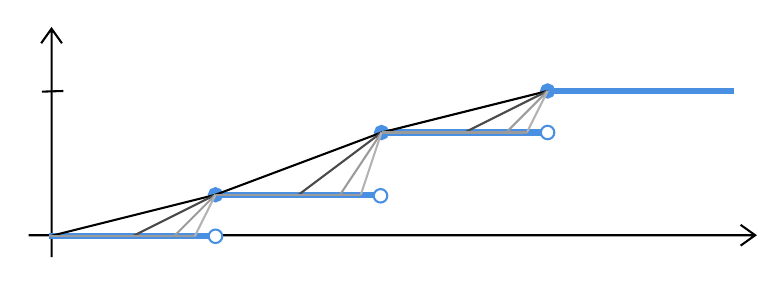
\begin{tikzpicture}[x=0.75pt,y=0.75pt,yscale=-1,xscale=1]
		%uncomment if require: \path (0,300); %set diagram left start at 0, and has height of 300
		
		%Shape: Axis 2D [id:dp9933169088018603] 
		\draw  (90,179.5) -- (440,179.5)(101,80) -- (101,190) (433,174.5) -- (440,179.5) -- (433,184.5) (96,87) -- (101,80) -- (106,87)  ;
		%Straight Lines [id:da6324835010323591] 
		\draw [color={rgb, 255:red, 74; green, 144; blue, 226 }  ,draw opacity=1 ][line width=2.25]    (100,180) -- (180,180) ;
		%Straight Lines [id:da43830458673578954] 
		\draw [color={rgb, 255:red, 74; green, 144; blue, 226 }  ,draw opacity=1 ][line width=2.25]    (180,160) -- (260,160) ;
		\draw [shift={(180,160)}, rotate = 0] [color={rgb, 255:red, 74; green, 144; blue, 226 }  ,draw opacity=1 ][fill={rgb, 255:red, 74; green, 144; blue, 226 }  ,fill opacity=1 ][line width=2.25]      (0, 0) circle [x radius= 2.14, y radius= 2.14]   ;
		%Straight Lines [id:da5946908786264795] 
		\draw [color={rgb, 255:red, 74; green, 144; blue, 226 }  ,draw opacity=1 ][line width=2.25]    (260,130) -- (340,130) ;
		\draw [shift={(260,130)}, rotate = 0] [color={rgb, 255:red, 74; green, 144; blue, 226 }  ,draw opacity=1 ][fill={rgb, 255:red, 74; green, 144; blue, 226 }  ,fill opacity=1 ][line width=2.25]      (0, 0) circle [x radius= 2.14, y radius= 2.14]   ;
		%Straight Lines [id:da6415810065034648] 
		\draw [color={rgb, 255:red, 74; green, 144; blue, 226 }  ,draw opacity=1 ][line width=2.25]    (340,110) -- (430,110) ;
		\draw [shift={(340,110)}, rotate = 0] [color={rgb, 255:red, 74; green, 144; blue, 226 }  ,draw opacity=1 ][fill={rgb, 255:red, 74; green, 144; blue, 226 }  ,fill opacity=1 ][line width=2.25]      (0, 0) circle [x radius= 2.14, y radius= 2.14]   ;
		%Shape: Circle [id:dp7079535511004624] 
		\draw  [color={rgb, 255:red, 74; green, 144; blue, 226 }  ,draw opacity=1 ][fill={rgb, 255:red, 255; green, 255; blue, 255 }  ,fill opacity=1 ] (176.75,180) .. controls (176.75,178.21) and (178.21,176.75) .. (180,176.75) .. controls (181.79,176.75) and (183.25,178.21) .. (183.25,180) .. controls (183.25,181.79) and (181.79,183.25) .. (180,183.25) .. controls (178.21,183.25) and (176.75,181.79) .. (176.75,180) -- cycle ;
		%Shape: Circle [id:dp356688862846672] 
		\draw  [color={rgb, 255:red, 74; green, 144; blue, 226 }  ,draw opacity=1 ][fill={rgb, 255:red, 255; green, 255; blue, 255 }  ,fill opacity=1 ] (256.25,160.5) .. controls (256.25,158.71) and (257.71,157.25) .. (259.5,157.25) .. controls (261.29,157.25) and (262.75,158.71) .. (262.75,160.5) .. controls (262.75,162.29) and (261.29,163.75) .. (259.5,163.75) .. controls (257.71,163.75) and (256.25,162.29) .. (256.25,160.5) -- cycle ;
		%Shape: Circle [id:dp4206679801509201] 
		\draw  [color={rgb, 255:red, 74; green, 144; blue, 226 }  ,draw opacity=1 ][fill={rgb, 255:red, 255; green, 255; blue, 255 }  ,fill opacity=1 ] (336.75,130) .. controls (336.75,128.21) and (338.21,126.75) .. (340,126.75) .. controls (341.79,126.75) and (343.25,128.21) .. (343.25,130) .. controls (343.25,131.79) and (341.79,133.25) .. (340,133.25) .. controls (338.21,133.25) and (336.75,131.79) .. (336.75,130) -- cycle ;
		%Straight Lines [id:da45930261671662476] 
		\draw [color={rgb, 255:red, 0; green, 0; blue, 0 }  ,draw opacity=1 ]   (100,180) -- (180,160) ;
		%Straight Lines [id:da5265683799675518] 
		\draw [color={rgb, 255:red, 0; green, 0; blue, 0 }  ,draw opacity=1 ]   (180,160) -- (260,130) ;
		%Straight Lines [id:da5731730383619638] 
		\draw [color={rgb, 255:red, 0; green, 0; blue, 0 }  ,draw opacity=1 ]   (260,130) -- (340,110) ;
		%Straight Lines [id:da8868699683693013] 
		\draw    (96.33,110.33) -- (106.67,110) ;
		%Straight Lines [id:da15958243221800172] 
		\draw [color={rgb, 255:red, 74; green, 74; blue, 74 }  ,draw opacity=1 ][fill={rgb, 255:red, 74; green, 74; blue, 74 }  ,fill opacity=1 ]   (140,180) -- (180,160) ;
		%Straight Lines [id:da14928807228415408] 
		\draw [color={rgb, 255:red, 74; green, 74; blue, 74 }  ,draw opacity=1 ][fill={rgb, 255:red, 74; green, 74; blue, 74 }  ,fill opacity=1 ]   (220,160) -- (260,130) ;
		%Straight Lines [id:da4546940909402881] 
		\draw [color={rgb, 255:red, 74; green, 74; blue, 74 }  ,draw opacity=1 ][fill={rgb, 255:red, 74; green, 74; blue, 74 }  ,fill opacity=1 ]   (300,130) -- (340,110) ;
		%Straight Lines [id:da9250256976836124] 
		\draw [color={rgb, 255:red, 155; green, 155; blue, 155 }  ,draw opacity=1 ]   (260,130) -- (300,130) ;
		%Straight Lines [id:da17471836932728624] 
		\draw [color={rgb, 255:red, 155; green, 155; blue, 155 }  ,draw opacity=1 ]   (180,160) -- (220,160) ;
		%Straight Lines [id:da3682988241261582] 
		\draw [color={rgb, 255:red, 155; green, 155; blue, 155 }  ,draw opacity=1 ]   (100,180) -- (170,180) ;
		%Straight Lines [id:da7640473574692048] 
		\draw [color={rgb, 255:red, 155; green, 155; blue, 155 }  ,draw opacity=1 ]   (160,180) -- (180,160) ;
		%Straight Lines [id:da24501668667345644] 
		\draw [color={rgb, 255:red, 155; green, 155; blue, 155 }  ,draw opacity=1 ]   (240,160) -- (260,130) ;
		%Straight Lines [id:da7034764353034018] 
		\draw [color={rgb, 255:red, 155; green, 155; blue, 155 }  ,draw opacity=1 ]   (320,130) -- (340,110) ;
		%Straight Lines [id:da6733906694024909] 
		\draw [color={rgb, 255:red, 182; green, 178; blue, 178 }  ,draw opacity=1 ]   (170,180) -- (180,160) ;
		%Straight Lines [id:da3446084332147836] 
		\draw [color={rgb, 255:red, 182; green, 178; blue, 178 }  ,draw opacity=1 ]   (250,160) -- (260,130) ;
		%Straight Lines [id:da679625623689905] 
		\draw [color={rgb, 255:red, 182; green, 178; blue, 178 }  ,draw opacity=1 ]   (330,130) -- (340,110) ;
		%Straight Lines [id:da17337341268860484] 
		\draw [color={rgb, 255:red, 155; green, 155; blue, 155 }  ,draw opacity=1 ]   (180,160) -- (250,160) ;
		%Straight Lines [id:da700392623544378] 
		\draw [color={rgb, 255:red, 155; green, 155; blue, 155 }  ,draw opacity=1 ]   (260,130) -- (330,130) ;
		
		
		
		
	\end{tikzpicture}
\end{figure}
	
\end{solution}

\begin{remark}
	In the question above, if there are no limitations that the sequence $ \set{\mu_n} $ should ave a density with respect to Lebesgue measure, then one natural choice is
	\[ \mu_n = \sum_{i}^{n} a_i \delta_i + (\sum_{i=n+1}^{\infty}a_i)\delta_{n+1}. \]
\end{remark}


\begin{problem}
	Let $ \mathcal{L}(Y) = \mu $, where $ \mu $ has continuous density $ f $. For $ n\in \N $, let $ Y_n = \ceil{nY}/n $, and let $ \mu_n = \mathcal{L}(Y_n) $.
	\begin{enumerate}[(a)]
		\item Describe $ \mu_n $ explicitly.
		\item Prove that $ \mu_n \Rightarrow \mu $.
		\item Is $ \mu_n $ discrete, or absolutely continuous, or neither? What about $ \mu $?
	\end{enumerate}
\end{problem}
\begin{solution}
	\begin{enumerate}[(a)]
		\item We start by calculating the cumulative distribution function for $ Y_n $.
		\begin{align*}
			F_n(y) &= \mu_n((-\infty,x]) = \prob(Y_n\in(-\infty,y]) \\
			&= \prob(\frac{\floor{nY}}{n}\in (-\infty,y]) \\
			&= \prob(\floor{nY}\in (-\infty,ny]) \\
			&= \prob(nY \in (-\infty,\floor{ny}+1))\\
			&= \prob(Y \in (-\infty,\frac{\floor{ny}}{n} + 1/n))\\
			&= \prob(Y \in (-\infty,\frac{\floor{nY}}{n}]) + \mu((\frac{\floor{ny}}{n},\frac{\floor{ny}+1}{n})) \\
			&= F(\frac{\floor{ny}}{n}) + \mu((\frac{\floor{ny}}{n},\frac{\floor{ny}+1}{n}))
 		\end{align*}
 		\item First observe that 
 		\[ \frac{\floor{ny}}{n} \to y \quad as \quad n\to\infty. \]
 		That is because $ \abs{\frac{\floor{ny}}{n} - y} = \frac{\abs{\floor{ny} - ny}}{n} \leq \frac{1}{n}. $ On the other hand
 		\[ \mu((\frac{\floor{ny}}{n},\frac{\floor{ny}+1}{n})) \to \mu((y,y)) = \mu(\emptyset) = 0 \quad as \quad n\to\infty. \]
 		So from part (a) we can see that
 		\[ F_n(y) \to F(y) \quad as \quad n\to\infty \]
 		for all $ y\in \R $. Thus $ \mu_n \Rightarrow \mu $ as $ n\to\infty $.
 		\item {\color{red} \noindent TODO: TO BE ADDED.}
	\end{enumerate}
\end{solution}


\begin{problem}
	Let $ 0 < M < \infty $, and let $ f,f_1,f_2,\cdots: [0,1] \to [0,M] $ be Borel-measurable functions with $ \int_{0}^{1}f\ d\lambda = \int_{0}^{1} f_n\ d\lambda = 1 $. Suppose $ \lim_n f_n(x) = f(x) $ for each fixed $ x\in [0,1] $. Define probability  measures $ \mu,\mu_1,\mu_2,\cdots $ by $ \mu(A) = \int_{A} f\ d\lambda $, and $ \mu_n(A) = \int_A f_n\ d\lambda $, for Borel $ A \subset [0,1] $. Prove that $ \mu_n \Rightarrow \mu $.
\end{problem}
\begin{solution}
	Let $ g: [0,1]\to\R $ be any bounded continuous function. Then by change of variable formula we have
	\[ \int g d\mu_n = \int_0^1 g f_n d\lambda, \qquad \int g d\mu = \int_0^1 gf d\lambda. \]
	Since $ f_n \to f $ pointwise, then $ gf_n \to gf $ pointwise as well. Observe that $ gf_n \leq gM $ and since $ g $ is bounded and continuous then $ \int gM d\lambda < \infty $. Thus by monotone convergence theorem we have
	\[ \int {gf_n} {d\lambda} \to \int gf d\lambda \quad \text{as $ n\to\infty $}. \]
	In other words $ \int g d\mu_n \to \int g d\mu $ as $ n\to\infty $. This proves that $ \mu_n \Rightarrow \mu $.
\end{solution}



\begin{problem}
	Let $ f:[0,1]\to (0,\infty) $ be a continuous function such that $ \int_{0}^{1}fd\lambda = 1 $ (where $ \lambda $ is Lebesgue measure on $ [0,1] $). Define probability measure $ \mu $ and $ \set{\mu_n} $ by $ \mu(A) = \int_{0}^{1}f\mathds{1}_A d\lambda $ and $ \mu_n(A) = \sum_{i=1}^{n}f(i/n)\mathds{1}_{A}(i/n)/\sum_{i=1}^{n}f(i/n) $.
	\begin{enumerate}[(a)]
		\item Prove that $ \mu_n \Rightarrow \mu $ as $ n\to\infty $.
		\item Explicitly construct  random variables $ Y $ and $ \set{Y_n} $ so that $ \mathcal{L}(Y)=\mu $, $ \mathcal{L}(Y_n)=\mu_n $, and $ Y_n\to Y $ with probability 1. 
	\end{enumerate}
\end{problem}
\begin{solution}
	\begin{enumerate}[(a)]
		\item Let $ A \in \mathcal{B} $ such that $ \mu(\partial A) = 0 $. Then
		\begin{align*}
			\lim_n \mu_n(A) &= \lim_n \frac{\sum_{i=1}^{n}f(i/n)\mathds{1}_{A}(i/n)}{\sum_{i=1}^{n}f(i/n)} \\
			&= \lim_n \frac{\sum_{i=1}^{n}f(i/n)\mathds{1}_{A}(i/n)1/n}{\sum_{i=1}^{n}f(i/n)1/n} \\
			&= \frac{\lim_n \sum_{i=1}^{n}f(i/n)\mathds{1}_{A}(i/n)1/n}{\lim_n \sum_{i=1}^{n}f(i/n)1/n} \\
			&= \frac{\int_{0}^{1} f \mathds{1} d\lambda}{\int_{0}^{1} f d\lambda} \\
			&= \int_{0}^{1}f\mathds{1}_A d\lambda  = \mu(A).
		\end{align*}
		Since $ A $ was arbitrary then $ \mu_n \Rightarrow \mu $ as $ n\to\infty $.
		
		\item From the definition of $ \mu $ and $ \mu_n $ we define $ F_n $ and $ F $ (the cumulative distribution functions) and then define the random variables $ Y, Y_1,Y_2,\cdots $ as
		\[ Y_n(\omega) = \sup_x\set{x: F_n(x)< \omega},\qquad Y(\omega)= \sup_x \set{x: F(x)<\omega}. \]
	\end{enumerate}
\end{solution}
\begin{remark}
	In Rosenthal, Theorem 7.2.1 defines the ``inverse'' of $ F $ as
	\[ Y(\omega) = \inf_x\set{x: F(x)\geq \omega}. \]
	{\color{red} \noindent  It is not clear to me }if these two definitions are the same or not. Because one of them leads to a left continuous function while the other one leads to a right continuous function.
\end{remark}


\section{Canonical Examples}
\begin{example}[Converging in probability but not almost surely]
	Let $ X, X_1,X_2,\cdots $ be random variables with $ X\equiv 0 $, and $ X_n = \mathds{1}_{B_n} $ for some $ B_n \in \mathcal{B} $ such that $ \prob(B)=1/n $. In other words $ \prob(X_n = 1) = 1/n $ and $ \prob(X_n=0) = 1-1/n $. Then 
	\begin{enumerate}[(a)]
		\item $ X_n \to X $ in probability.
		\item $ X_n \not\to X $ almost surly. (Because $ 1/n $ is not summable). 
	\end{enumerate}
\end{example}
\begin{remark}
	\begin{enumerate}[(a)]
		\item Defining $ B_n $ such that $ \prob(B_n) =1/n^2 $ then we will also have the almost sure convergence.
		\item Defining $ X_n = n\mathds{1}_{B_n} $ with $ \prob(B_n)=1/n $, then $ X_n\to X $ in probability, and $ 1 = \E{X_n} \not\to \E{X} = 0 $.
		\item Defining $ X_n = n^2\mathds{1}_{B_n} $ with $ \prob(B_n)=1/n^2 $, then $ X_n\to X $ almost surely, but $ 1 = \E{X_n} \not\to \E{X} = 0. $
	\end{enumerate}
\end{remark}


\begin{example}[Convergence in distribution but not in probability]
	Let $ X,X_1,X_2,\cdots $ be i.i.d. random variables each equal to $ \pm 1 $ with probability $ 1/2 $. Then obviously $ \mu_n \Rightarrow \mu $ however $ X_n $ does not converge to $ X $ in probability. For instance, let $ \epsilon=2 $. Then $ \prob(\abs{X_n-X}\geq 2) = 1/2 \not\to 0 $.
\end{example}


\begin{example}
	We give an example of a sequence of random variables which is unbounded, uniformly integrable, and undominated (in the sense of the hypothesis of dominated convergence theorem). Define
	\[ \Omega = \N,\quad \prob(\Omega)=2^{-\omega},\quad X_n(\omega) = \frac{2^n}{n}\delta_{\omega,n} \]
\end{example}


\begin{observation}
	Let $ x\in \R $. Then $ 1-x < e^{-x} $. This is a very important inequality that can be justified by simply looking at the graph of $ (1-x) $ and $ e^{-x} $. This inequality is used in the proof of the Borel-Cantelli lemma, as well as in Problem \autoref{prob:DiscreteSpaceIndependentEvents}.
\end{observation}


\begin{observation}[]
	Recall the definition of $ \limsup $ and $ \liminf $ of a sequence of events $ A_1,A_2,\cdots $
	\[ \limsup_n A_n = \bigcap_{n=1}^{\infty} \bigcup_{k=n}^{\infty} A_k, \qquad \liminf_n A_n = \bigcup_{n=1}^{\infty}\bigcap_{k=n}^\infty A_n. \]
	The important observation is that
	\[ \set{\bigcap_{k=n}^{\infty}A_n}  \nearrow \liminf_n A_n, \qquad \set{\bigcup_{k=n}^\infty A_n} \searrow \limsup_n A_n. \]
\end{observation}



\newpage
\section{Interesting Questions and Remarks From Other Books}
This section will contain the interesting questions and remarks collected from other books. The content will be cited.


\subsection{Normal Numbers, Coin Tossing, WLLN, and SLLN}
This subsection contains a brief summary of the interesting story in Billingsley section 1.1. This story is interesting because it contains most of the main ideas under one umbrella demonstrates most of the interesting concepts at once.

The story begins by the notion of length for half open intervals as a subset of $ [0,1] $. Let $ (a,b] $ be such an interval. The notion of length for this interval is 
\[ \ell((a,b]) = b-a.\]
Now let $ \Omega $ be the space of all infinitely long binary strings. For instance $ \omega = 01110101 \in \Omega $. Each point in $ \Omega $ can be thought of as an experiment in which we toss a coin infinitely many times. For instance $ \omega $ given above corresponds to the experiment where on the first toss we got a Tails, on the second toss we got a heads, and etc. Consider the set $ A_0 \subset \Omega $ given by
\[ A_0 = \set{\omega: d_1(\omega ) = 0}.  \]
Similarly we can define 
\[ A_{10} = \set{\omega: d_1(\omega)=1, d_2(\omega)=0}, \]
and etc. We associate each $ \omega\in\Omega $ with a real number as follows
\[ \Omega \ni u_1u_2u_3\cdots \quad \longleftrightarrow \quad 0.u_1u_2u_3\cdots \in [0,1]. \tag{\halfnote} \]
With this association it is easy to check that for instance we have
\[ A_{10} \ \longleftrightarrow \ (\frac{1}{2},\frac{3}{4}], \ A_{101} \ \longleftrightarrow\ (\frac{5}{8},\frac{6}{8}],\quad  \text{and etc.} \]
And in general
\[ A_{u_1\cdots u_n} \ \longleftrightarrow\ (0.u_1\cdots u_n, 0.u_1\cdots u_n + \frac{1}{2^n}]. \]
With an slightly different point of view, we can get a very clear understanding of the weak law of large numbers, as well as the strong law of large numbers. Let $ d_n:[0,1] \to \set{0,1} $ be the ``$ i^\text{th} $ component function in base 2''. For instance $ d_2(0.01101\cdots) = 1 $ as the second position in the binary expansion is 1. The graph of $ d_n $ is depicted in the following figure for few different values of $ n $.
\begin{figure}[h!]
	\centering
	\includegraphics[width=0.5\linewidth]{Images/components}
	\label{fig:components}
\end{figure}
\FloatBarrier
Now assume that in our coin tossing experiment, we are interested in the total number of Heads. For instance in $ \omega = 1010100\dots $, where the sequence of 0s continue in the tail, the number of Heads is 3. This can also be calculated by the function $ H_n:[0,1]\to\N $ given as
\[ H_n = \sum_{i=1}^n d_i, \]
that gives the number of heads in the first $ n $ trials. So for the example above, the number of heads are also given as $ H_8(0.1010100\dots) = d_1(0.1010100\dots) + d_2(0.1010100\dots) + d_3(0.1010100\dots) + \cdots + 0 = 1 + 0 + 1 + 0 + 1 + 0 + 0 + \cdots + 0  = 3 $. So the 1-1 correspondence between $ \Omega $ and $ [0,1] $ in $ (\halfnote) $ is a very useful correspondence. That is because most of the events of interests on $ \Omega $ can be converted back to some intervals on $ [0,1] $ for which we can assign probability. For another example, we want to know the behaviour of the fraction of heads as the number of experiments goes to infinity. For $ \omega \in \Omega $, the fraction of heads in the $ n $ first trials is
\[ F_n(\omega) = \frac{1}{n}\sum_{i=1}^{n} d_i(\omega) = \frac{H_n(\omega)}{n}. \]
Consider the following example.
\begin{example}
	In an infinite coin tossing experiment what is the probability that the sum of first three tosses is 2 (i.e. 2 heads appear in the first 3 trials?)
\end{example}
\begin{solution}
	Consider the pre-image $ 2 $ under $ F_3 $. I.e.
	\[ \inv{F_3}(2) = (\frac{3}{8},\frac{4}{8}] \cup (\frac{5}{8},\frac{6}{8}] \cup (\frac{6}{8},\frac{7}{8}]. \]
	The length of $ \inv{F_3}(2) $ is $ 3/8 $. So we can assign the probability $ 3/8 $ to this set. 
\end{solution}

The graph of the set functions $ F_n $ is very illustrative as in the following figure
\begin{figure}[h!]
	\centering
	\includegraphics[width=0.6\linewidth]{Images/FractionRandomVariable}
	\label{fig:fractionrandomvariable}
\end{figure}
\FloatBarrier
The graph of the functions $ F_n $ shows that $ F_n $ the ``deviation'' of the sequence of function from $ 1/2 $ gets more and more ``negligible''. Mathematically, for any $ \epsilon>0 $ (in the figure above $ \epsilon=1/4 $) we have
\[ \prob(\abs{F_n - 1/2}\geq \epsilon)\to 0 \quad \text{as } n\to\infty. \]
This is shown in the figure below
\begin{figure}[h!]
	\centering
	\includegraphics[width=0.5\linewidth]{Images/convergenceInProb}
	\label{fig:convergenceinprob}
\end{figure}
\FloatBarrier
This is the Weak Law of Large Numbers! In fact, more is true with our coin tossing experiment. For ``almost all'' of the points $ \omega \in [0,1] $ we have
\[ F_n(\omega) \to 1/2 \quad \text{as}\ n\to\infty. \]
The meaning of ``almost all'' is that the set of all points $ \eta \in [0,1] $ such that $ F_n(\eta)\not\to 1/2 $ is ``negligible''. This is the Borel's Normal Numbers Theorem.






\subsection{Solved Problems}

\begin{problem}[From Billingsley]
	\label{prob:DiscreteSpaceIndependentEvents}
	\begin{enumerate}[(a)]
		\item Show that a discrete probability space (see Example 2.8 for the formal definition) can not contain an infinite sequence $ A_1,A_2,\cdots $ of independent events each of probability $ 1/2 $. Note that $ A_n $ ve be identified with heads on the $ n $-the toss of a coin. 
		\item Suppose that $ 0\leq p_n \leq 1 $. and put $ \alpha_n = \min(p_n,1-p_n) $. Show that if $ \sum_n a_n $ diverges, then no discrete probability space can contain independent events $ A_1,A_2,\cdots $ such that $ A_n $ has probability $ p_n $.
	\end{enumerate}
\end{problem}

\begin{solution}
	\begin{enumerate}
		Let $ \set{x} \subset \Omega $. Then $ x $ belongs to only one of the four disjoint sets below
		\[ A_1\cap A_2,\quad A_1^c\cap A_2 \quad A_1\cap A_2^c,\quad A_1^c \cap A_2^c. \]
		Observe that the probability of each of these events are $ 1/4 $ (noting that if $ A,B $ are independent then $ A^c, B^c $ are independent as well). So $ \set{x} $ must have probability $ 1/4 $ at most. Now consider the events $ A_1,A_2,A_3 $. Then $ x $ should belong to only one of the disjoint events below
		\begin{align*}
			A_1\cap A_2\cap A_3, \quad A_1\cap A_2^c\cap A_3, \quad A_1\cap A_2\cap A_3^c, \quad A_1\cap A_2^c\cap A_3^c, \\
			A_1^c\cap A_2\cap A_3, \quad A_1^c\cap A_2^c\cap A_3, \quad A_1^c\cap A_2\cap A_3^c, \quad A_1^c\cap A_2^c\cap A_3^c. 
		\end{align*}
		Since $ A_1,A_2,A_3 $ are independent events the probability of each of the events above are $ 1/8 $. So $ \set{x} $ can have probability $ 1/8 $ at most. Continuing this we will get $ \prob(\set{x}) = 0 $ for all $ x\in \Omega $. On the other hand since $ \Omega $ is countable then 
		\[ 1 = \prob(\Omega ) = \sum_{x\in \Omega} \prob(\set{x}) = 0 \]  
		which is a contradiction. 
		
		
		\item When $ p_n $ goes to zero fast enough such that $ \sum_n p_n <\infty $, then $ A_n $ can be independent events on a discrete probability space. To see this let $ B_i $ be $ A_i $ or $ A_i^c $ for each $ i $. Then 
		\[ \prob(B_1\cap \cdots\cap B_n) \leq \prod_{i=1}^{n}(1-\alpha_i) \leq e^{-\sum_{i=1}^{n}\alpha_i}. \]
		Thus when the sum $ \sum_i \alpha_i $ diverges the RHS goes to zero and this leads to conclusion that $ \prob(\set{x}) = 0 $ for all $ x\in \Omega $ which leads to a similar kind of contradiction we had in part (a). But when $ \sum_i\alpha_i $ is converging, then we don't have a contradiction which leads to the conclusion that such independent events can exist.
	\end{enumerate}
\end{solution}

\begin{remark} 
	\begin{enumerate}[(i)]
		\item Note that by discrete probability measure we also require it to be countable.
		\item In part (b) of the question above we use an argument very similar to the one in the proof of Borel-Cantelli. However, it is not yet clear for me if we can somehow directly use Borel-Cantelli Lemma.
	\end{enumerate}
\end{remark}


\begin{problem}[From Ross]
	Ben can talk a course in compute science or chemistry. If she takes the computer science course, then she will get A grade with probability $\frac{1}{2}$. If she takes the chemistry course, then she will get A grade with probability $\frac{1}{3}$. She decides to base her decision on the flip of a fair coin. What is the probability that she gets an A in chemistry?
\end{problem}
\begin{solution}
	We define the following events
	\begin{quote}
		$A$: she will get an A grade.\\
		$CO$: she will take the computer science course.\\
		$CH$: she will take the chemistry course.
	\end{quote}
	Then the question is basically asking for $\prob(A \cap CH)$. We can compute it by
	\[ \prob(A \cap CH) = \prob(A|CH)\prob(CH) = \frac{1}{3}\cdot\frac{1}{2} = \frac{1}{6}. \]
\end{solution}

\begin{problem}
	And urn contains seven black balls and five white balls. We draw two times from the urn. Given that the each ball has the same probability to be drawn, what is the probability that both balls drawn are black?
\end{problem}
\begin{solution}
	This question nicely demonstrates the fact that there are many ways to define the event spaces, and not all of them are very useful in computing the desired probability. Define
	\begin{quote}
		$E$: two drawn balls are black.
	\end{quote}
	The question is in fact asking $\prob(E)$. But this even is not very useful in any progress with the solution. Thus we need to define some finer events
	\begin{quote}
		$E_1$: The first drawn ball is black.\\
		$E_2$: The second drawn ball is black.
	\end{quote}
	It is clear that $E = E_1 \cap E_2$. These two finer events allows us to compute the probability of interest given the data we have in our hand.
	\[ \prob(E_1 \cap E_2) = \prob(E_2 | E_1) \prob(E_1) = \frac{6}{11} \cdot \frac{7}{12} \]
\end{solution}

\begin{problem}[From Ross]
	Three men at a party through their hats into the center of the room, and then, after mixing the hats, each pick a hat randomly. What is the probability if non of them get their own hat back.
\end{problem}
\begin{solution}
	There are a million ways to tack a probability problem. We can construct a suitable sample space and then compute the probabilities explicitly, or we can use the properties of the probability function to computer the desired probability without any need to construct the sample space. Here, we will demonstrate two ways.
	
	\textbf{Solving the problem by utilizing the properties of the probability function.} First we need to define some suitable events. There are again many ways to define event sets and each have their own pros and cons. We proceed with the following definition.
	\begin{quote}
		$E_i$: The person $i$ ``selects'' his own hat.  
	\end{quote}
	Also, with this particular construction of the event sets, it is much more easier to compute the complementary probability of the desired probability first and then compute the desired one by simply subtracting it from 1. The complement of the event ``no men gets his own hat back'' is ``at least one man gets his hat back'' which is $\prob(E_1\cup E_2 \cup E_3)$. To compute the terms of this we first need to calculate $\prob(E_i)$, $\prob(E_i \cap E_j)$ where $i\neq j$ and also $\prob(E_1 \cap E_2 \cap E_3)$. We know that $\prob(E_i) = 1/3$ for $i=1,2,3$. That is because it is equally likely he selects any of the hats at the center. For $\prob(E_i\cap E_j)$ we can write
	\[ \prob(E_i\cap E_j) = \prob(E_i|E_j)\prob(E_j) = \frac{1}{2}\cdot \frac{1}{3} =  \frac{1}{6}.   \]
	In which we used the fact that $\prob(E_i|E_j)$ is $\frac{1}{2}$ for distinct $i,j$. That is because given person $j$ selects his hat correctly, then there are two possibilities for $E_i$ to select his hat (he can pick the correct one or the wrong one). Lastly for $\prob(E_1\cap E_2\cap E_3)$ we write
	\[ \prob(E_1\cap E_2\cap E_3) = \prob(E_1|E_2\cap E_3)\prob(E_2\cap E_3) = \prob(E_1|E_2\cap E_3) \prob(E_2 | E_3) \prob(E_3) = 1 \cdot \frac{1}{2} \cdot \frac{1}{3} = \frac{1}{6}.  \]
	Thus 
	\[ \prob(E_1 \cup E_2 \cup E_3) = (1) - (1/2) + (1/6) = \frac{4}{6}. \]
	Then the probability of interest will be
	\[ \prob(E) = 1-\frac{4}{6} = \frac{1}{3}. \]
	
	\textbf{Solving by constructing a sample space.} A suitable sample space for this problem can be the set of all permutations on three letters. This set is
	\[ \Omega = 
	\set{\begin{pmatrix}
			a & b & c \\
			\boxed{a} & \boxed{b} & \boxed{c}
		\end{pmatrix},
		\begin{pmatrix}
			a & b & c \\
			\boxed{a} & c & b
		\end{pmatrix},
		\begin{pmatrix}
			a & b & c \\
			b & a & \boxed{c}
		\end{pmatrix},
		\begin{pmatrix}
			a & b & c \\
			b & c & a
		\end{pmatrix},
		\begin{pmatrix}
			a & b & c \\
			c & a & b
		\end{pmatrix},
		\begin{pmatrix}
			a & b & c \\
			c & \boxed{b} & a
	\end{pmatrix}}.
	\]
	Note that the elements in the box represents the fixed point of the permutation. The probability of interest is basically the number of permutations that has no fixed point. As it is clear from the set $\Omega$, the probability is
	\[ \prob(E) = \frac{2}{6} = \frac{1}{3}. \]
\end{solution}

\begin{problem}[Conditional probability mass function (from Ross)]
	Let $ X,Y $ be two random variables with the joint probability mass function given as 
	\[ P(1,1) = 0.5 \qquad P(1,2)=0.1,\qquad P(2,1)=0.1, \qquad P(2,2)=0.3. \]
	Calculate the conditional probability mass function of $ X $ given that $ Y = 1 $.
\end{problem}
\begin{solution}
	We will use the following identity
	\[ P_{X|Y}(x|y) = \prob(X=x|Y=y) = \frac{\prob(X=x,Y=y)}{\prob(Y=y)}. \]
	Observe that 
	\[ \prob(Y=y) = \sum_x \prob(Y=y,X=x) \]
	thus $ \prob(Y=1) = 0.5 + 0.1 = 0.6. $
	So we will have
	\[ P_{X|Y}(1|1) = \frac{0.5}{0.6} = \frac{5}{6}, \qquad P_{X|Y}(2|1) = \frac{0.1}{0.6} = \frac{1}{6}. \]
\end{solution}

\begin{problem}[Conditional probability mass function for geometric random variables (from Ross)]
	Let $ X_1,X_2 $ be two independent random variables with geometric distributions with parameters $ (n_1,p) $ and $ (n_2,p) $. Calculate the conditional probability mass function of $ X_1 $ given that $ X_1+X_2 = m $.
\end{problem}
\begin{solution}
	First, observe that $ Y = X_1 + X_2 $ is a binomial distribution with parameter $ (n_1+n_2, p) $. Thus we can write
	\[ P_{X_1|Y}(k|m) = \prob(X_1 = k | Y = m) = \frac{\prob(X_1 = k, X_1+X_2 = m)}{\prob(X_1+X_2 = m)} = \frac{\prob(X_1=k, X_2 = m-k)}{\prob(Y = m)} \]
	Since the random variables $ X_1 $ and $ X_2 $ are independent, we can write
	\[ P_{X_1|Y}(k|m) = \frac{\prob(X_1=k)\prob(X_2 = m-k)}{\prob(Y=m)} = \frac{\binom{n_1}{k}\binom{n_2}{m-k}}{\binom{n_1+n_2}{m}}. \]
\end{solution}

\begin{problem}[Conditional probability mass function for Poisson random variables (from Ross)]
	Let $ X,Y $ be two independent Poisson random variables with parameters $ \lambda_1 $ and $ \lambda_2 $ respectively. Calculate the conditional probability mass function for $ X $ given that $ X_1 + X_2 = n $.
\end{problem}
\begin{solution}
	First observe that $ Z = X + Y $ is a Poisson random variable with parameter $ \lambda_1 + \lambda_2 $. Thus we will have
	\[ P_{X|X+Y}(m|n) = \frac{\prob(X=m|X+Y=n)}{\prob(X+Y = n)} = \frac{\prob(X=m,Y=n-m)}{\prob(X+Y = n)} \]
	Given that $ X,Y $ are independent random variables then we can write
	\[ P_{X|X+Y}(m,n) = \frac{\prob(X=m)\prob(Y=n-m)}{\prob(X+Y=n)} = \frac{\lambda_1^n \lambda_2^{n-m}n!}{m!(n-m)!(\lambda_1+\lambda_2)^n} = \binom{n}{m} (\frac{\lambda_1}{\lambda_1+\lambda_2})^m ( \frac{\lambda_2}{\lambda_1+\lambda_2})^{n-m} \]
	Thus the conditional probability mass function of $ X $ given that $ X+Y = n $ will be a binomial random variable with parameter $ (n,\lambda_1/(\lambda_1+\lambda_2)) $. We can now easily compute the conditional expectation value as
	\[ \E{X|X+Y = n} = \frac{n\lambda_1}{\lambda_1 + \lambda_2} \]
\end{solution}

\begin{problem}
	Let $ X,Y $ be two discrete random variables. Prove that 
	\[ \E{\E{X|Y}} = \E{X}. \]
\end{problem}
\begin{solution}
	We start with the definition of the expectation of a discrete random variable.
	
	\begin{align*}
		\E{\E{X|Y}} &= \sum_y \E{X|Y=y} \prob(Y=y) = \sum_y \sum_x x\prob(X=x|Y=y)\prob(Y=y) \\
		& = \sum_{x,y} x\prob(X=x,Y=y) = \sum_x x \sum_y \prob(X=x,Y=y) = \sum_x x\prob(X=x) = \E{X}
	\end{align*}
\end{solution}

\begin{problem}[The expectation of a random number of random variables (from Ross)]
	Let the expected number of injures in an industrial field be 4 per week. Also, assume that the number of workers injured at each incidence are independent random variables with average 2. Then what is the expected number of injuries in one week?
\end{problem}
\begin{solution}
	Let $ X_1,X_2,\cdots $ be i.i.d random variables representing the number of workers injured at each incidence. We are interested in 
	\[ \E{X_1+\cdots+X_N} \]
	where $ N $ is a random variable representing the number of incidences occurred in a week. By the law of conditional expectation we can write
	\[ \E{X_1 + \cdots + X_N} = \sum_n \E{X_1+\cdots+X_n}\prob(N=n) = \sum_n n\E{X} \prob(N=n) = \E{X} \E{N}.\]
	Thus the average number of workers injured in a week will be 8. 
\end{solution}

\begin{problem}[An alternative way to compute the expectation of a geometric random variable]
	Consider a coin with probability $ p $ to fall heads. What is the expectation value of the number of tosses required until we get the first head?
\end{problem}
\begin{solution}
	Let $ X_1,X_2,\cdots $ be Bernoulli random variables with parameter $ p $. Let $ N $ be a random variable denoting the number of tosses required until we get the first heads. We can condition the expected value of $ E $ to the first outcome.
	\[ \E{N} = \E{N|X_1 = H }\underbrace{\prob(X_1 = H)}_{=p} + \E{N|X_1=T}\underbrace{\prob(X_1=T}_{=1-p})  \]
	Observe that 
	\[ \E{N|X_1=H} =1 ,\qquad \E{N|X_1=T} = 1+\E{N}.\]
	Thus we will have
	\[ \E{N} = \frac{1}{p}. \]
\end{solution}

\begin{problem}[Trapped miner (from Ross)]
	A miner is trapped in the mine and has three doors in front of him. He is equally likely to choose any of the three. The first door will take him to safety after 2 hours of walking, the second door will take him to the mine again after 3 hours of walking, and the third door will take him to the mine again after 5 hours of walking. What is the expected time that the miner will arrive to safety?
\end{problem}
\begin{solution}
	Let $ X_1,X_2,\cdots $ be random variables denoting the doors that the miner choose at each time that he attempts to escape. Furthermore, let $ T $ be a random variable showing the the time it takes for the miner to escape. To calculate $ \E{T} $ we can condition it on the first door choice. I.e.
	\[ \E{T} = \E{T|X_1 =1}\prob(X_1=1) + \E{T|X_1 =2}\prob(X_1=2)+\E{T|X_1 =3}\prob(X_1=3) \]
	Observe that 
	\[ \prob(X_1=1) = \prob(X_1=2) = \prob(X_1=3) = 1/3. \]
	Also
	\[  \E{T|X_1 =1} = 2,\qquad  \E{T|X_1 =2} = 3+\E{T}, \qquad \E{T|X_1 =3} = 3+\E{T}. \]
	Thus we will have
	\[ \E{T} = 10. \]
	So on average it will take the miner to exit the mine in 10 hours. Note that this does not guarantee that the miner will eventually escape. It is possible that we will get in trap by repeatedly choosing the door number 3.
\end{solution}

\begin{problem}[From Rosenthal]
	Suppose that $ \Omega = \set{1,2}, $ with $ \prob(\emptyset) = 0 $ and $ \prob(\set{1,2}) = 1 $. Suppose $ \prob(\set{1}) = \frac14 $. Prove that $ \prob $ is countably additive if and only if $ \prob(\set{2})=\frac34 $.
\end{problem}
\begin{solution}
	The proof has two parts
	\begin{itemize}
		\item [$ \boxed{\Longrightarrow} $] Since $ \prob $ is countably additive, then 
		\[ \prob(\set{1} \dot\cup \set{2}) = \prob(\set{1}) + \prob(\set{2}) = 1. \]
		This implies $ \prob(\set{2}) = 3/4 $.
		\item [$ \boxed{\Longleftarrow} $] Assume $ \prob(\set{2}) = 3/4 $. Then it is very straightforward to check that for every disjoint subset $ A,B \subset \Omega $, we have
		\[ \prob(A \dot\cup B) = \prob(A) + \prob(B). \]
		Thus we conclude that $ \prob $ is countably additive.
	\end{itemize}
\end{solution}

\begin{problem}[From Rosenthal]
	Suppose $ \Omega = \set{1,2,3} $ and $ \mathcal{F} $ is a the collection of all subsets of $ \Omega $. Find (with proof) necessary and sufficient conditions on the real numbers $ x,y,z $ such that there exists a countably additive probability measure $ \prob $ on $ \mathcal{F} $ such that $ x = \prob\set{1,2}, y=\prob\set{2,3}, z=\prob\set{1,3} $.
\end{problem}
\begin{solution}
	To find the necessary conditions, we assume that $ \prob $ is an additive probability measure. Let $ a = \prob\set{1}, b=\prob\set{2} $, and $ c = \prob\set{3} $. Then the countable additivity implies
	\[ a+b=x,\qquad b+c=y,\qquad a+c=z. \]
	Then due to countable additivity, and the fact that $ \prob $ is a probability measure (i.e. $ \prob\set{1,2,3} = 1 $), we have $ a+b+c = 1 $, thus we need to have
	\[ x+y+z = 2. \tag{\eighthnote} \]
	Further, we solve the $ a,b,c $ in terms of $ x,y,z $ are require the singleton probabilities to be positive. We have
	\[ a = \frac{x-y+z}{2},\qquad b = \frac{x+y-z}{2},\qquad c=\frac{-x+y+z}{2}. \]
	One of the necessary conditions is also to have
	\[ x-y+z\geq0,\qquad x+y-z\geq0,\qquad -x+y+z \geq0. \tag{\twonotes}  \]
	The two conditions ($ \eighthnote $) and $ (\twonotes) $  together are the necessary and sufficient conditions for $ \prob $ to be a valid probability measure.
\end{solution}

\begin{problem}[From Rosenthal]
	Suppose that $ \Omega = \N $ is the set of positive integers, and $ \prob $ is defined for all $ A\subseteq \Omega $ by $ \prob(A) = 0 $ if $ A $ is finite, and $ \prob(A) = 1 $ if $ A $ is infinite. Is $ \prob $ finitely additive?
\end{problem}
\begin{solution}
	Not it is not. Consider the partitioning of the set $ \Omega $ by the even $ E $ and odd $ O $ integers.
	\[ \prob(\Omega) = \prob(E) + \prob(O) \implies 1 = 2, \]
	which is not true. Thus $ \prob $ is not finitely additive.
\end{solution}

\begin{problem}[From Rosenthal]
	Suppose that $ \Omega = \N $, and $ \prob $ is defined for all $ A \subseteq \Omega $ by $ \prob(A) = \abs{A} $ if $ A $ is finite, and $ P(A)=\infty $ if $ A $ is infinite.  This $ P $ is of course not a probability measure (in fact it is counting measure), however we can still ask the following: (be the convention $ \infty+\infty = \infty $)
	\begin{enumerate}[(I)]
		\item Is $ \prob $ finitely additive?
		\item Is $ \prob $ countably additive?
	\end{enumerate}
\end{problem}
\begin{solution}
	\begin{enumerate}[(I)]
		\item Yes. $ \prob $ being finitely additive is equivalent being additive for disjoint $ A,B \subset \Omega $. There are three cases for these choices
		\begin{enumerate}[(i)]
			\item $ A,B $ are both finite. In this case $ \prob(A\dot\cup B) = \prob(A) + \prob(B) $ since $ 0=0+0 $.
			\item $ A,B $ are both infinite. In this case $ \prob(A\dot\cup B) = \prob(A) + \prob(B) $ since $ \infty+\infty = \infty $.
			\item One of the sets $ A,B $ is infinite. Then $ \prob(A\dot\cup B) = \prob(A) + \prob(B) $ since $ 0+\infty = \infty. $
		\end{enumerate}
		\item No. We will show this by counterexample. We can write $ \Omega = \dot\bigcup_{i\in \N}\set{i} $. Then the countable additivity implies
		\[ \prob(\Omega) = \prob(\dot\bigcup_{i\in \N}\set{i}) \implies 1 = 0.\]
		which is not true.
	\end{enumerate}
\end{solution}


\begin{problem}[From Rosenthal]
	Let $ \mathcal{I} $ be the set of all intervals in $ [0,1] $ (open, closed, half-open, singleton, empty set). Show that $ \mathcal{I} $ is a semi-algebra.
\end{problem}
\begin{solution}
	By definition of $ \mathcal{I} $ we have $ \emptyset\in \mathcal{I} $. Let $ A_1, A_2 $ be two intervals in $ [0,1] $. If $ A_1,A_2 $ are disjoint, then $ A_1\cap A_2 \in \mathcal{I} $. If they are not disjoint, then without loss of generality we can assume that 
	\[ A_1 = \set{x\in[0,1]\ |\ a<x<b}, A_2 = \set{x\in[0,1]\ |\ c<x<d}, \]
	where $ a<c<b<d $. Thus $ A_1\cap A_2 = (c,b) $. So $ \mathcal{I} $ is closed under finite intersection. The proof is the same for any other choices of $ A_1,A_2 $ (i.e. being closed set, etc). To show the third property, again, without the loss of generality, let $ A = (a,b) $. Then $ A^c = (-\infty,a] \dot\cup [b,\infty) $. For other choices of $ A $ (i.e. being closed, etc) we will have a similar argument. Thus we conclude that the collection $ \mathcal{I} $ is a semi-algebra of the subsets of $ [0,1] $.
\end{solution}

\begin{problem}[From Rosenthal]
	Let $ \mathcal{I} $ be the semi-algebra consisting of all intervals in $ [0,1] $. Define
	\[ \mathcal{B}_0 = \set{\text{all finite unions of elements of $ \mathcal{I} $}.} \]
	Show that $ \mathcal{B}_0 $ is not a $ \sigma\text{-algebra} $.
\end{problem}
\begin{solution}
	Along with many other sets, $ \mathcal{I} $ contains all of the singletons, so does $ \mathcal{B}_0 $. Consider the following collection
	\[ \mathcal{A} = \set{\set{x}\ :\ x \in \Q \cap [0,1]}. \]
	By definition, all of the sets in the collection $ \mathcal{A} $ belongs to $ \mathcal{B}_0 $. However, the following countable union
	\[ \dot\bigcup_{A \in \mathcal{A}} A = [0,1] \cap \Q \]
	does not belong to $ \mathcal{B}_0 $ (as it is not possible to generate with only finite unions of the elements of singletons in $ \mathcal{I} $).
\end{solution}

\begin{problem}[From Rosenthal]
	Prove that the outer measure $ \prob^* $ is countably sub-additive, i.e.
	\[ \prob^*(\bigcup_{n=1}^{\infty} B_n) \leq \sum_{n=1}^{\infty} \prob^*(B_n) \qquad \text{for any $ B_1,B_2,\cdots \in \Omega $}.\]
\end{problem}
\begin{solution}
	This problem is the proof of Lemma 2.3.6 in Rosenthal. See the text for more context. A very quick review on the context is that we have a semi-algebra $ \mathcal{I} $ of the subsets of $ \Omega $, and we have the function $ \prob: \mathcal{I} \to [0,1] $ that satisfies the properties required for the extension theorem, hence there exist a valid probability space $ (\Omega, \mathcal{M}, \prob^*) $, where $ \mathcal{M} $ is a $ \sigma\text{-algebra} $ and $ \prob^* $ is a probability measure (which is also the outer measure). The proof of this question is as follows. 
	
	Fix $ \epsilon>0 $. Since the outer measure is the infimum of the sum of the probabilities on all $ \mathcal{I} $ covers, then for each $ B_n $ we can find a collection $ \set{C_{nk}} $ where $ C_{nk}\in\mathcal{I} $ such that 
	\[ \sum_k \prob(C_{nk}) \leq \prob^*(B_n) + \epsilon2^{-n}. \]
	On the other hand, since $ \set{C_{nk}}_{nk} $ covers $ \bigcup_n B_n $, then again from the properties of inf we have
	\[ \prob^*(\bigcup_n B_n) \leq \sum_{nk} \prob(C_{nk}). \]
	combining these two we will get
	\[  \prob^*(\bigcup_n B_n) \leq \sum_n \prob^*(B_n) + \epsilon. \]
	Since this is true for all $ \epsilon>0 $, then it implies that 
	\[  \prob^*(\bigcup_n B_n) = \sum_n \prob^*(B_n). \]
\end{solution}

\begin{problem}[From Rosenthal]
	\label{prob:countableAdditivity}
	If $ A_1,A_2,\cdots \in \mathcal{M} $ are disjoint, then prove that 
	\[ \prob^*(\dot\bigcup_n A_n) = \sum_n \prob^*(A_n). \]
\end{problem}
\begin{solution}
	First, we start to show the finite additivity, and then using the properties of monotnonicity and sub-additivity, we will prove the countable additivity as well. Let $ A_1, A_2 \in \mathcal{M} $ disjoint. In particular, since $ A_1 \in \mathcal{M} $, from the definition of $ \mathcal{M} $ (see page 12 Rosenthal), then
	\[ \prob^*(A_1 \cup A_2) = \prob^*(A_1^c \cap (A_1\cup A_2)) + \prob^*(A_1 \cap (A_1 \cup A_2)) = \prob^*(A_2) + \prob^*(A_1). \]
	This implies that for any finite disjoint collection of $ A_i $ we have the additivity property (by induction). Now for any $ m \in \N $ we have
	\[  \sum_{n<m} \prob^*(A_n)  = \prob^*(\bigcup_{n\leq m}A_n)  \leq \prob^*(\bigcup_n A_n) \]
	where the last inequality follows form the monotnonicity property of $ \prob^* $. Since this is true for all $ m \in \N $, then we conclude that 
	\[ \prob^*(\bigcup_n A_n) \geq \sum_n \prob^*(A_n). \]
	On the other hand, from the sub-additivity property we have
	\[ \prob^*(\bigcup_n A_n) \leq \sum_n \prob^*(A_n). \]
	These two implies that 
	\[ \prob^*(\bigcup_n A_n) = \sum_n \prob^*(A_n). \]
\end{solution}

\begin{problem}[From Rosenthal]
	Let $ \mathcal{M} $ be the $ \sigma\text{-algebra} $ we get from the extension theorem, where by definition it contains all of the sets like $ A \in \Omega $ for which the outer measure is additive on the union of $ A \cap E $ and $ A^c \cap E $ for $ \forall E \subset \Omega  $. In other words
	\[ \mathcal{M} = \set{A \subseteq \Omega\ :\ \prob^*(A\cap E) + \prob^*(A^c \cap E) = \prob^*(E) \quad \text{for all } E \subset \Omega}. \]
	Prove that $ \mathcal{M} $ is an algebra.
\end{problem}
\begin{solution}
	Let $ A = \Omega $. Then
	\[ \prob^*(A \cap E) + \prob^*(A^c\cap E) = \prob^*(E) + \prob^*(\emptyset) = \prob^*(E). \]
	So we conclude that $ \Omega \in \mathcal{M} $. Also, it follows immediately from the definition of $ \mathcal{M} $ that if $ A \in \mathcal{M} $ then $ A^c \in \mathcal{M} $. Now it remains to show if $ A_1, A_2 \in \mathcal{M} $ then $ A_1\cap A_2 \in \mathcal{M} $. Let $ E \subset \Omega $. Then 
	\begin{align*}
		&\prob^*(E \cap (A_1 \cap A_2)) + \prob^*(E \cap (A_1 \cap A_2)^c ) \\
		&= \prob^*(E\cap (A_1\cap A_2)) + \prob^*(E\cap A_1^c \cap A_2) + \prob^*(E\cap A_1 \cap A_2^c) + \prob^*(E\cap A_1^c \cap A_2^c) \\
		&\leq \prob^*(E\cap A_1\cap A_2) + \prob^*(E \cap A_1^c \cap A_2) + \prob^*(E \cap A_1 \cap A_2^c) + \prob^*(E\cap A_1^c \cap A_2^c)\\
		&=\prob^*(E\cap A_2) + \prob^*(E\cap A_2^c) \qquad \text{(because $ A_1 \in \mathcal{M} $)} \\
		&=\prob^*(E) \qquad \text{(because $ A_2 \in \mathcal{M} $)}.
	\end{align*}
	On the other hand, from the sub-additivity property we know that 
	\[ \prob^*(E\cap (A_1\cap A_2)) + \prob^*(E \cap (A_1\cap A_2)^c) \geq \prob^*(E). \]
	Thus we conclude that 
	\[ \prob^*(E\cap (A_1\cap A_2)) + \prob^*(E\cap (A_1\cap A_2)^c) = \prob^*(E). \]
	This implies that $ A_1\cap A_2 \in \mathcal{M} $ and this finishes the proof.
\end{solution}


\begin{problem}[From Rosenthal]
	Let $ A_1,A_2,\cdots \in \mathcal{M} $ be disjoint. For each $ m\in \N $, let $ B_m = \bigcup_{n\leq m} A_n $. Prove that for all $ m\in \N $, and for all $ E \subseteq \Omega $ we have
	\[ \prob^*(E\cap B_m) = \sum_{n\leq m} \prob^*(E\cap A_n). \]
\end{problem}
\begin{solution}
	First, observe that this statement is true for $ m=1 $ in a trivial way. For $ m=2 $, since $ A_2 \in \mathcal{M} $, then we can expand $ E\cap B_2 $ according to $ A_2 $, i.e.
	\[ \prob^*(E\cap B_2) = \prob^*((E\cap B_2)\cap A_2) + \prob^*((E \cap B_2)\cap A_2^c) \]
	On the other hand $ (E\cap B_2)\cap A_2 = E \cap A_2 $ and $ (A\cap B_2)\cap A_2^c = E\cap B_1 = E\cap A_1 $. Thus we can write
	\[ \prob^*(E\cap B_2) = \prob^*(E\cap A_1) + \prob^*(E\cap A_2). \]
	In general, for $ m \in \N $ we can write
	\[ \prob^*(E\cap B_m) = \prob^*(E\cap A_m) + \prob^*(E\cap B_{m-1}). \]
	Thus using induction we can write
	\[ \prob^*(E\cap B_m) = \sum_{n\leq m }\prob^*(E\cap A_n). \]
\end{solution}

\begin{problem}[From Rosenthal]
	In this question covers some of the proves for constructing a uniform probability measure on $ \Omega = [0,1] $. Let $ \mathcal{I} $ be the set of all intervals in $ \Omega $, and let $ \mathcal{P}:\mathcal{I} \to [0,1] $ be a function that assigns the length of an interval to that interval. We want to prove that $ \mathcal{P} $ satisfies the property (2.3.3) of extension theorem (2.3.1) in Rosenthal. I.e. we want to prove that for $ A, A_1,\cdots \in \mathcal{I} $ such that $ A \subset \cup_{i}A_i$ satisfies 
	\[ \prob(A) \leq \sum_{i} \prob(A_i). \]
\end{problem}
\begin{solution}
	We will do this in three parts. 
	\begin{enumerate}[(i)]
		\item Step 1. First, we prove that for any finite $ A, A_1,\cdots,A_n \in\mathcal{I} $ collection where $ A \subset \cup_{i=1}^{n} A_i $ we have
		\[ \prob(A) \leq \sum_{i=1}^{n} \prob(A_i). \]
		To see this let $ A_1,A_2, A \in \mathcal{I} $ such that $ A \subset A_1 \cup A_2 $. We also assume that $ A_1\cap A \neq \emptyset $ as well as $ A_2 \cap A \neq \emptyset $. This is to ensure that we do not have redundant interval in our collection that does not cover $ A $. Note that from any collection of intervals we can put aside the redundant intervals and do our reasoning here and then finally at the last step consider the redundant intervals as well. So our assumption above does not lose the generality of the proof. Let $ a_i, b_i $ represent the left (right) endpoints of the intervals $ A_i $ and $ a_0,b_0 $ represent the left (right) endpoints of the interval $ A $. In order to the intervals $ A_1, A_2 $ to cover $ A $ white neither of them are redundant we need to have
		\[ \min\set{a_1,a_2} \leq a_0 \leq a_2 \leq b_1 \leq b_0 \leq \max\set{b_1,b_2}. \]
		Then it follows that 
		\[ b_0 - a_0 \leq (b_1 - a_1) + (b_2 - a_2). \]
		Thus this implies that 
		\[ \prob(A) \leq \prob(A_1) + \prob(A_2). \]
		We can generalize this by induction to any finite number of intervals.
		\item Step 2. We now want to prove that for any countable \emph{open} intervals $ A_1,A_2,\cdots \in \mathcal{I} $ such that $ A \subset \cup_n A_n $ for $ A \in \mathcal{I} $ closed, we have
		\[ \prob(A) \leq \sum_n \prob(A_n). \]
		To see this, we will use the Heine-Borel theorem. Since the collection $ \set{A_1,A_2,\cdots} $ is an open cover for the closed set $ A $. if $ A $ is the whole space $ \Omega $, then the inequality that we want to show follows immediately (LHS is 1 while RHS is infinite). However, if $ A $ is not the whole space, then it is bounded. Thus $ A $ is closed and bounded, hence compact (by Heine-Borel). So the open cover has a finite sub-cover and this completes the proof by reducing this case to case (i) above.
		\item Step 3. We now want to show that if $ A_1,A_2,\cdots \in \mathcal{I} $ is any countable collection of intervals, and if $ A \subset \cup_n A_n $ for any $ A \in \mathcal{I} $ then 
		\[ \prob(A) \leq \sum_{i=1}^\infty\prob(A_i).  \]
		{\color{red} \noindent TODO: TO BE COMPLETED}
	\end{enumerate}
	
\end{solution}


\begin{problem}[From Rosenthal]
	Let $ \mathcal{A} = \set{(-\infty,x]\ :\ x\in \R} $. Prove that $ \sigma(\mathcal{A}) = \mathcal{B} $, i.e. that the smallest $ \sigma $-algebra of subsets of $ \R $ which contains $ \mathcal{A} $ is equal to the Borel $ \sigma $-algebra of subsets of $ \R $.
\end{problem}
\begin{solution}
	By definition, we know that $ \mathcal{B} $ is the smallest $ \sigma\text{-algebra} $ that contains all of the intervals. However, we claim that the $ \sigma\text{-algebra} $ $ \sigma(\mathcal{A}) $ also contains all of intervals. To see this, let $ I $ be an interval which will have different cases $(-\infty,a),(-\infty,a],(a,b),[a,b],(a,b],[a,b),(a,\infty),[a,\infty) $. Each of these sets can be constructing by using the sets in $ s \sigma(\mathcal{A}) $ and using its sigma-algebra properties. Thus we showed that $ \sigma(\mathcal{A}) $ contains $ \mathcal{I} $ the set of all intervals. However, by definition $ \mathcal{B} $ was the smallest $ \sigma\text{-algebra} $ containing all of intervals. Thus the $ \sigma\text{-algebra} $ generated by $ \mathcal{A} $ (i.e. the smallest $ \sigma\text{-algebra} $ by definition) is equal to $ \mathcal{B} $. 
\end{solution}

\begin{problem}[From Rosenthal]
	Prove the following statements. 
	\begin{enumerate}[(a)]
		\item Prove that the Cantor set $ K $ and its complement $ K^c $ is in $ \mathcal{B} $, the Borel set of the subset of $ [0,1] $.
		\item Prove that $ K,K^c \in \mathcal{M} $, where $ \mathcal{M} $ is the $ \sigma\text{-algebra} $ by the extension applied for the uniform distribution on $ [0,1] $ (see theorem 2.4.4 Rosenthal).
		\item Prove that $ K^c \in \mathcal{B}_1 $ where $ \mathcal{B}_1 $ is defined by (2.2.6) Rosenthal (i.e. the set of all finite or countable unions of intervals $ \mathcal{I} $).
		\item Prove that $ \mathcal{B}_1 $ is not a $ \sigma\text{-algebra} $.
		
	\end{enumerate}
\end{problem}
\begin{solution}
	\begin{enumerate}[(a)]
		\item In the construction of the cantor set, at each step we remove the middle 1/3 of the intervals. So starting with $ I_0 = [0,1] $ at the first step we will get $ I_1 =  [0,1/3]\cup[2/3,1] $, etc. The Cantor set is $ I_0 \cap I_1 \cap I_2 \cap \cdots $. Since $ I_i \in \mathcal{B} $ for all $ i \in \N $, and $ \mathcal{B} $ is a $ \sigma\text{-algebra} $ and is closed under countable intersection, then $ K \in \mathcal{B} $ as well. It follows immediately that $ K^c \in \mathcal{B} $ as well, as $ \mathcal{B} $ is closed under complement.
		\item Since $ \mathcal{M} \supset \mathcal{B}$, and as we showed above that $ K,K^c \in \mathcal{B} $, then $ K,K^c \in \mathcal{M} $ as well.
		\item From the construction given in part (a), we have
		\[ K = I_0 \cap I_1 \cap I_2 \cap \cdots. \]
		From the De Morgan's law we will have
		\[ K^c = I_0^c \cup I_1^c \cup I_2^c \cup \cdots. \]
		Thus by definition of $ \mathcal{B}_1 $ we have $ K^c \in \mathcal{B}_1 $.
		\item First, observe that (see Rosenthal page 17) that the Cantor set is uncountable. So there is no way to construct it by finite or countable union of singletons (which are in $ \mathcal{I} $). We can not construct it with the finite or countable union of any intervals as $ K $ is a nowhere dense set. I.e. for every interval $ (a,b) \in \mathcal{I} $ containing $ x \in K $ there exists, $ y\in \R $ such that $ y \notin K $. To put this precisely, let $ I_1,I_2,I_3,\cdots $ is collection of intervals such that $ I = \cup_n I_n $. Since $ K $ is nowhere dense, for any $ I_i $ in the collection that contains $ x \in K $ we can find some $ y \in \R $ that $ y \notin K $. This is a contradiction and we have $ I \subset \cup_n I_n $.
		\item As we saw above, $ K^c \in \mathcal{B}_1 $ but $ K \notin \mathcal{B}_1 $. Thus $ \mathcal{B}_1 $ is not closed under complement, thus it is not a $ \sigma\text{-algebra} $.
	\end{enumerate}
\end{solution}

\begin{problem}[An extension of the extension theorem (from Rosenthal)]
	Let $ \mathcal{I} $ be a semialgebra of subsets of $ \Omega $. Let $ \prob:\mathcal{I}\to [0,1] $ with $ \prob(\emptyset) = 0 $ and $ \prob(\Omega) = 1 $, satisfying 
	\[ \prob(\bigcup_n A_n) \geq \sum_n \prob(A_n)\ \qquad \text{for $ A_1,A_2,\cdots \in \mathcal{I} $ \emph{disjoint}, and $ \bigcup_n A_n \in \mathcal{I} $}, \]
	as well as 
	\[ \prob(A) \leq \prob(B), \qquad A \subseteq B, \]
	and
	\[ \prob(\bigcup_n B_n) \leq \sum_n \prob(B_n) \qquad \text{for $ B_1,B_2,\cdots \in \mathcal{I} $, and $ \bigcup_n B_n \in \mathcal{I} $}.\]
	Then there exist a valid probability space $ (\Omega, \mathcal{M},\prob^*) $ such that $ \prob $ and $ \prob^* $ agree on the elements of $ \mathcal{I} $
\end{problem}
\begin{solution}
	According to the extension theorem 2.3.1 we need to prove that these alternative statements implies $ 2.3.3 $. Let $ A, A_1,A_2,\cdots \in \mathcal{I} $ (note that the union of $ A_i $s do not belong to $ \mathcal{I} $ necessarily). Define
	\[ B_n = A_n \cap A. \]
	Then we will have $ A = \cup_n B_n $, thus $ \cup_n B_n \in \mathcal{I} $. So
	\[ \prob(A) = \prob(\bigcup_n B_n) \leq \sum_n \prob(B_n) \leq \sum_n \prob(A_n). \]
\end{solution}
\begin{observation}
	In the prove above, one might attempt 
	\[ \prob(A) \leq \prob(\bigcup_i A_i) \leq \sum_i \prob(A_i) \]
	where for the first inequality we use the monotnonicity (as $ A \subset \bigcup_i A_i $) and for the second inequality we use the countable sub additivity given in the statement of the theorem. However, this prove is \emph{wrong!}. Because we are not allowed to use the second inequality, as it does not satisfies the requirements for the sub-additivity statement to work. That is because $ \bigcup_n A_n $ may not be in $ \mathcal{I} $ necessarily.
\end{observation}

\begin{problem}[Uniqueness property of the extension theorem (from Rosenthal)]
	Let $ \mathcal{I},\prob, \prob^* $ be the same as in Theorem 2.3.1 (Rosenthal). Let $ \mathcal{F} $ be any $ \sigma\text{-algebra} $ with $ \mathcal{I} \subseteq \mathcal{F} \subseteq \Omega $. Let $ \Q $ be any probability measure on $ \mathcal{F} $, such that $ \Q(A) = \prob(A) $ for all $ A \in \mathcal{I} $. Then prove that $ \Q(A) = \prob^*(A) $ for all $ A \in \mathcal{F} $.
\end{problem}
\begin{solution}
	Let $ A \in \mathcal{F} $, and $ A_i \in \mathcal{I} $ for $ i=1,2,\dots $ such that $ A \subseteq \bigcup_i A_i $. Since $ \Q $ is a probability measure, then 
	\[ \Q(A) \leq \Q(\bigcup_i A_i) \leq \sum_i \Q(A_i). \]
	Then we can write
	\begin{align*}
		\prob^*(A) &= \inf_{\substack{A_1,A_2,\cdots \in \mathcal{I} \\ A \subseteq \bigcup_i A_i}}\sum_i \prob(A_i) \\
		&= \inf_{\substack{A_1,A_2,\cdots \in \mathcal{I} \\ A \subseteq \bigcup_i A_i}}\sum_i \Q (A_i) \\
		&\geq \inf_{\substack{A_1,A_2,\cdots \in \mathcal{I} \\ A \subseteq \bigcup_i A_i}}\Q(\bigcup_i A_i)\\
		&\geq \inf_{\substack{A_1,A_2,\cdots \in \mathcal{I} \\ A \subseteq \bigcup_i A_i}}\Q(A)\\
		& = \Q(A).
	\end{align*}
	However, we could do the same with $ A^c \in \mathcal{F} $, which would lead to
	\[ \prob^*(A^c) \geq \Q(A^c). \]
	Since $ \prob^*(A^c) = 1 - \prob^*(A) $ and $ \Q(A^c) = 1 - \Q(A) $, then this implies  $  \prob^*(A) \geq \Q(A)  $. Thus $ \prob^*(A) = \Q(A) $.
\end{solution}


\begin{problem}[Properties of Random Variables (from Rosenthal)]
	\label{prob:capcupcapcup}
	Prove the followings.
	\begin{enumerate}[(i)]
		\item If $ X,Y $ are random variables and $ c\in\R $, then $ X+c, cX, X^2, X+Y,  $ and $ XY $ are random variables. 
		\item If $ Z_1,Z_2,\cdots $ are random variables such that $ \lim_{n\to \infty} Z_n(\omega) $ exists for all $ \omega\in \Omega $,, and $ Z(w) = \lim_{n\to \infty}Z_n(\Omega) $, then $ Z $ is also a random variable.
	\end{enumerate}
\end{problem}

\begin{solution}
	the proves are as follows.
	\begin{enumerate}[(i)]
		\item \begin{enumerate}[(a)]
			\item $ \inv{(X+c)}((-\infty,x]) = \set{w\ :\ X(w)+c \leq x} = \set{w\ :\ X(w)\leq x-c} = \inv{X}((0\-\infty,x-c]) \in \mathcal{F} $.
			\item Assume $ c\neq 0 $. Then $ \inv{(cX)}((-\infty, x]) = \set{w\ :\ cX(w) \leq x} = \set{w\ :\ X(w) \leq x/c}  = \inv{X}((-\infty,x/c]) \in \mathcal{F}. $ For the case were $ c=0 $, then $ cX \equiv 0 $ on all $ \Omega $, and this is a random variable as $ (\inv{cX})((0,x]) = \emptyset$ if $ x < 0 $ and $ (\inv{cX})((0,x]) = \Omega $ if $ x\geq 0 $.
			\item $ X^2((-\infty,a]) = \set{w\ :\ X^2 \leq a} = \set{w\ :\ X \in [-\sqrt{a},\sqrt{a}]} \in \mathcal{F} $.
			\item $ \inv{(X+Y)}((\infty,x]) = \set{w\ :\ X(w)+Y(w) < x} = \bigcup_{r\in \Q}(\set{X < r} \cap \set{Y<x-r}) $. Since this is a countable union, thus in $ \mathcal{F} $.
			\item I have the following prove but I am not sure if it is a correct one or not. I feel that this is a correct proof as there seems to be nothing that can make it not to work.
			\[ \inv{(XY)}((-\infty,x]) = \set{XY < x} = \bigcup_{n\in\N} (\set{X<n} \cap \set{Y<x/n}). \]
			The following prove is the idea by Rosenthal. Once we know that $ X^2 $, $ X+Y $, and $ cX $ are random variables, then we can deduce $ XY $ is also a random variable as
			\[ XY = \frac{1}{2}((X+Y)^2 - X^2 - Y^2)) \]
		\end{enumerate}
		\item In a nutshell this statements claims that the point-wise convergence of a sequence of random variables is a random variable. We need to show that the event $ \set{Z\leq r} \in \mathcal{F} $. To see this, let $ w \in \set{Z\leq r} $. This means that $ Z(w) \leq r $. Since $ Z_n(\omega) \to Z(\omega) $ as $ n\to \infty $, then this implies that $ \forall m \in \N $ there exists $ N \in \N $ such that $ \forall n > N $ we have $ Z_n(\omega) \leq r + \frac{1}{m} $. Thus we can write
		\[ \set{Z(w) \leq r} = \bigcap_{m=1}^{\infty} \bigcup_{N=1}^{\infty} \bigcap_{n=N}^{\infty} \set{ Z_n(\omega) \leq r + \frac{1}{m}} \]
	\end{enumerate}
\end{solution}

\begin{problem}
	Let $ f:\R \to \R $ be continouse or piece-wise continuous function. Then $ f $ is a Borel function.
\end{problem}
\begin{solution}
	We first prove the statement for a continuous function. To show that $ f $ is a Borel function we need to show $ \inv{f}(B) \in \mathcal{B} $ for $ B \in \mathcal{B}$. Since the pre-image preserves the union, intersection, and complements, and by definition for a continuous function the pre-image of an open set is an open set, and using the fact that we can write any Borel set as a countable intersection, union, or complements of open sets then we conclude that $ \inv{f}(B) \in \mathcal{B} $.
	A second way to show this is observe that $ \inv{f}((x,\infty)) \in \mathcal{B} $ as $ (x,\infty) $ is open and $ f $ is continuous, thus its pre-image is also an open set thus a Borel set. Then its complement is also a Borel set, i.e.
	\[ (\inv{f}((x,\infty)))^c = \inv{f}((-\infty,x]) \in \mathcal{B}. \]
	Thus shows that $ f $ is a Borel function (since the pre-image of $ (0,x] $ is a Borel set.
	
	For the case where $ f $ is piece-wise continuous, by the definition of the piece-wise continuoity, $ f $ has at most countably many discontinuities. The we can write $ f $ as 
	\[ f(x) = f_1(x)\mathds{1}_{I_1}(x) + f_2(x)\mathds{1}_{I_2}(x) + f_3(x)\mathds{1}_{I_3}(x)  + \cdots + f_n(x)\mathds{1}_{I_n}(x),  \]
	where $ I_1,I_2,I_3\cdots,I_n  $ are disjoint intervals on which $ f_1,f_2,f_3,\cdots, f_n $ are continuous respectively. By the statement for the first part of the proof, we know that $ f_i $ is a Borel function (since it is continuous) as well as the indicator function $ \mathds{1}_{I_i} $. Their multiplication is also a Borel function and the sum of these Borel functions is a also a Borel function, thus $ f(x) $ is a Borel function.
\end{solution}

\begin{problem}
	Prove that if $ A,B $ are two independent events, then $ (A^c, B) $, $ (A,B^c) $, and $ (A^c, B^c) $ are pairwise independent.
\end{problem}
\begin{solution}
	Since $ A,B $ are independent, then $ \prob(A\cap B) = \prob(A) \prob(B)$. From the identity $ B = (B\cap A) \dot\cup (B\cap A^c) $. From the properties of the probability measure we have
	\[ \prob(B) = \underbrace{\prob(A\cap B)}_{\prob(A)\prob(B)} + \prob(A^c \cap B). \]
	Then we can write
	\[ \prob(A^c\cap B) = \prob(B) - \prob(A\cap B) = \prob(B) (1-\prob(A)) = \prob(B)\prob(A^c). \]
	Thus $ A^c,B $ are also independent events. We use a similar argument for $ A,B^c $. To show that the events $ A^c, B^c $ are also independent, we use the inclusion-exclusion principle. 
	\[ \prob(A^c\cap B^c) = 1 - \prob(A\cup B) = 1 - (\prob(A)+\prob(B) - \prob(A)\prob(B)) = (1-\prob(A))(1-\prob(B))=\prob(A^c)\prob(B^c). \]
	Another way of showing this without the inclusion-exclusion principle is to use the identity
	\[ A^c = (A^c\cap B) \dot\cup (A^c\cap B^c). \]
	Then 
	\[ \prob(A^c) = \underbrace{\prob(A^c\cap B)}_{\prob(A^c)\prob(B)} + \prob(A^c\cap B^c). \]
	We can write
	\[ \prob(A^c \cap B^c) = \prob(A^c)(1-\prob(B)) = \prob(A^c) \prob(B^c).  \]
\end{solution}
\begin{problem}
	Let $ X,Y $ be random variables, and $ f,g : \R \to \R $ be Borel functions. Then if $ X,Y $ are independent, $ f(X) $ and $ g(X) $ are also independent.
\end{problem}
\begin{solution}
	Since $ X,Y $ are independent, thus for any $ S_1,S_2 \in \mathcal{B} $ we have
	\[ \prob(\set{X \in S_1}\cap \set{Y\in S_2}) = \prob(\set{X\in S_1}) \prob(\set{Y \in S_2}). \]
	Consider
	\[ \prob(\set{f(X) \in S_1} \cap \set{g(Y) \in S_2})=\prob(\set{X \in \inv{f}(S_1)} \cap \set{Y \in \inv{g}(S_2)}) = \prob(\set{f(X) \in S_1}) \prob(\set{g(Y) \in S_2}). \]
	The equality above hods because for any $ S_1, S_2 \in \mathcal{B} $ we have $ \inv{f}(S_1),\inv{g}(S_2) \in \mathcal{B} $, that is because $ f,g $ are Borel functions.
\end{solution}

\begin{problem}[Continuity of probabilities]
	Prove that the probability measure function is continuous from bellow and above. I.e. for the continuity from below, let $ A, A_1, A_2,\cdots \in \mathcal{F} $ such that  $ \set{A_n}\nearrow A $, i.e. $ A_1 \subseteq A_2 \subseteq \cdots $ and $ A = \bigcup_n A_n $. Then $ \lim_{n\to \infty} \prob(A_n) = \prob(A) $. For the continuity from above, let $ A,A_1,A_2,\cdots \in \mathcal{F} $ such that $ \set{A_n}\searrow A $, i.e. $ A_1\subseteq A_2\subseteq \cdots $ and $ A = \bigcap_n A_n $, then $ \lim_{n\to \infty}\prob(A_n) = \prob(A) $.
\end{problem}
\begin{solution}
	First, we prove the probability from below. In general, one can observe that if $ \set{A_n}\nearrow A $, then $ \set{\prob(A_n)} $ indeed converges as this is a bounded monotone sequence in $ \R $. However, to show that this sequence converges to $ \prob(A) $, we do as following. Consider the following sets
	\[ B_1 = A_1, \qquad B_2 = A_2 \backslash A_1, \qquad B_3 = A_3 \backslash A_2, \cdots. \]
	Then $ A = \dot\cup B_n $. Thus $ \prob(A) = \sum_{n=1}^{\infty}\prob(B_n) $. Thus the series on the rand hand side converges. This implies that the corresponding partial sums also converges. However, by the construction we have
	\[ \prob(A_1) = \prob(B_1),\quad \prob(A_2) = \prob(B_1) + \prob(B_2)+ \cdots. \]
	Thus the converges of the partial sums implies the convergence of $ \set{\prob(A_n)} $.
	
	For the proof for the continuity from above, first observe that if for a collection $ A,A_1,A_2,\cdots \in \mathcal{F} $ we have $ \set{A_n} \searrow A $, then this is equivalent to $ \set{A^c_n}\nearrow A^c $. This follows from the De Morgan's law as well as the change of the direction of the inclusion $ \subseteq $ under taking complements. By hypothesis we have $ \set{A_n}\searrow A $, which is equivalent to$ \set{A^c_n}\nearrow A^c $. From the first part of the proof, it follows that $ \lim_{n\to \infty}\prob(A^c_n) = \prob(A^c) $. Thus
	\[ \lim_{n\to \infty}(1-\prob(A_n)) = 1 - \prob(A). \]
	Note that $ \prob(A_n) $ converges to some real number as $ n\to \infty $, because it is a bounded decreasing sequence. Thus by the laws of the limit we can write
	\[1 -  \lim_{n\to\infty} \prob(A_n) = 1 - \prob(A). \]
	Then it follows that 
	\[ \lim_{n\to \infty}\prob(A_n) = \prob(A). \]
\end{solution}

\begin{problem}[From Rosenthal]
	Let $ A_1,A_2,\cdots,A_n \in \mathcal{F} $. Generalize the principle of inclusion-exclusion to:
	\[ \prob(A_1\cup\cdots\cup A_n) = \sum_{i=1}^n A_i - \sum_{1\leq i < j \leq n} \prob(A_i \cap A_j) + \sum_{1\leq i < j < k \leq n} \prob(A_i \cap A_j \cap A_k) - \cdots \pm \prob(A_1\cap \cdots \cap A_n). \]
	\emph{Hint: Expand $ 1 - \prod_{i=1}^n (1-\mathds{1}_{A_i}) $, and take expectation of both sides.}
\end{problem}
\begin{solution}
	First, observe that $ \mathds{1}_{A^c} = 1 - \mathds{1}_A $. So
	\[ 1 - \prod_{i=1}^n(1-\mathds{1}_{A_i}) = 1 - \prod_{i=1}^n \mathds{1}_{A_i^c} = 1 - \mathds{1}_{A_1^c\cap\cdots\cap A_n^c} = \mathds{1}_{A_1\cup\cdots\cup A_n}.  \]
	On the other hand, 
	\[ 1 - \prod_{i=1}^n (1-\mathds{1}_{A_i}) = \sum_{i=1}^{n}\mathds{1}_{A_i}  - \sum_{1 \leq i < j \leq n} \mathds{1}_{A_i \cap A_j} + \cdots \pm \mathds{1}_{A_1\cap\cdots\cap A_n}.  \]
	So we have
	\[ \mathds{1}_{A_1\cup\cdots\cup A_n} = \sum_{i=1}^{n}\mathds{1}_{A_i}  - \sum_{1 \leq i < j \leq n} \mathds{1}_{A_i \cap A_j} + \cdots \pm \mathds{1}_{A_1\cap\cdots\cap A_n}. \]
	By applying the expectation to both sides we will get
	\[ \prob(A_1\cup\cdots\cup A_n) = \sum_{i=1}^n A_i - \sum_{1\leq i < j \leq n} \prob(A_i \cap A_j) + \sum_{1\leq i < j < k \leq n} \prob(A_i \cap A_j \cap A_k) - \cdots \pm \prob(A_1\cap \cdots \cap A_n). \]
\end{solution}

\begin{problem}[From Rosenthal]
	Let $ f(x) = ax^2 + bx + c $ be a second-degree polynomial function where $ a,b,c \in \R $.
	\begin{enumerate}[(a)]
		\item Find necessary and sufficient condition on $ a,b $ and $ c $ such that the equation $ \E{f(\alpha x)} = \alpha^2 \E{f(X)} $ holds for all $ \alpha \in \R $ and all random variable $ X $. 
		\item Find necessary and sufficient condition on $ a,b $ and $ c $ such that the equation $ \E{f(x-\beta)} = \E{f(x)} $ holds of all $ \beta \in \R $ and all random variable $ X $.
		\item Do parts $ (a) $ and $ (b) $ account for the properties of the variance function? Why or why not?
	\end{enumerate}
\end{problem}
\begin{solution}
	\begin{enumerate}[(a)]
		\item For the LHS we have
		\[ \E{\alpha^2 a x^2 + \alpha b x + c} = a\alpha^2 \E{x^2} + b\alpha \E{x} + c. \]
		And for the RHS we have
		\[ \alpha^2\E{f(x)} = a\alpha^2\E{x^2} + b\alpha^2 \E{x} + c\alpha^2. \] 
		Thus the necessary and sufficient condition for the equality to hold for every $ \alpha \in \R $ is to have
		\[ b = 0, \qquad c = 0. \]
		\item For the LHS we have
		\[ \E{f(x-\beta)} = a\E{x^2} + (b - 2a\beta)\E{x} + a\beta^2 - b\beta + c.  \]
		For the RHS we have
		\[ \E{f(x)} = a\E{x^2} + b\E{x} + c. \]
		This implies that we need to have 
		\[ a = 0, \qquad b = 0. \]
		I.e. the polynomial should be a constant polynomial.
		\item For the property $ \operatorname{Var}{(\alpha C)} = \alpha^2 \operatorname{Var}{(C)} $, it follows from the fact that in part (b) we found that for the polynomial we need to have $ b = 0 $ and $ c = 0 $. However, part (b) does not account for the property of variance that $ \operatorname{Var}(X+b) = \operatorname{Var}(X) $. Because in the case of $ \operatorname{Var} $ the constants of the polynomial depends on the random variable under consideration. I.e. we have
		\[ b = - 2 \E{X}, \qquad c = \E{X}^2. \]
	\end{enumerate}
\end{solution}

\begin{problem}[From Rosenthal]
	Let $ X_1,X_2,\cdots $ be independent, each with mean $ \mu $ and variance $ \sigma^2 $, and let $ N $ be an integer-valued random variable with mean $ m $ and variance $ v $, with $ N $ independent of all the $ X_i $. Let $ S = X_1 + X_2 + \cdots + X_n = \sum_{i=1}^{\infty} X_i \mathds{1}_{N\geq i} $. Compute $ \operatorname{Var}(S) $ and $ \E{S} $.
\end{problem}
\begin{solution}[Using the conditional expectation]
	For this problem we can either use the conditional expectation or use the first principles.
	\[ \E{S} = \E{X_1+\cdots+X_N} = \sum_n \E{X_1+\cdots+X_n}\prob(N = n) = \mu \sum_n n \prob(N=n) = \mu m. \] 
	Similarly we have
	\begin{align*}
		\E{S^2} &= \sum_n \E{S^2\ |\ N = n} \prob(N=n) \\
		&= \sum_n \E{(X_1+\cdots+X_n)^2} \prob(N=n) \\
		&= \sum_n \E{\sum_i X_i^2 + \sum_{i<j}X_iX_j} \prob(N=n) \\ 
		&= \sum_n (\sum_i \E{X_i^2} + 2\sum_{i<j}\E{X_iX_j}) \prob(N=n) \\
		&= \sum_n ((\sigma^2 + \mu^2)n + n(n-1)\mu^2) \prob(N=n)\\
		&= (\sigma^2 + \mu^2)m + \mu^2(v+m^2 - m).
	\end{align*}
	Where we have used $ \E{X_i^2} = \operatorname{Var}(X_i) + \E{X_i}^2 = \mu^2 + \sigma^2 $, and also used the fact that the sum $ \sum_{i<j} $ has $ \binom{n}{2} $ terms.
	Now we can compute the variance
	\[ \operatorname{Var}(S) = \E{S^2} - \E{S}^2 = (\sigma^2 + \mu^2)m + \mu^2(v+m^2 - m) - \mu^2 m^2 = \sigma^2 m + \mu^2 v. \]
\end{solution}
\begin{problem}[from Rosenthal]
	Let $ X,Z $ be independent random variables each with standard normal distribution. Let $ a,b\in \R $ (not both 0), and let $ Y = aX + bZ $.
	\begin{enumerate}[(a)]
		\item Compute $ \operatorname{Corr}(X,Y) $.
		\item Show that $ \abs{\Corr(X,Y)} \leq 1 $.
		\item Given necessary and sufficient conditions on the values of $ a $ and $ b $ such that $ \Corr(X,Y) = 1 $.
		\item Given necessary and sufficient conditions on the values of $ a $ and $ b $ such that $ \Corr(X,Y) = -1 $.
	\end{enumerate}
\end{problem}
\begin{solution}
	\begin{enumerate}[(a)]
		\item First, observe that 
		\[ \E{X} = \E{Z} = 0, \quad \Var(X) = \Var(Y) = 1, \quad \E{Y} = a+b, \quad \Var(Y) = a^2 + b^2 \]
		where we have used the properties of variance to compute $ \Var(Y) $. By the definition of correlation we have
		\[ \Corr(X,Y) = \frac{\operatorname{Cov}(X,Y)}{\sqrt{\Var(X)\Var(Y)}} = \frac{\E{XY} - \E{X}\E{Y}}{\sqrt{a^2+b^2}} = \frac{a}{\sqrt{a^2+b^2}}. \]
		
		\item It follows immediately by
		\[ \abs{\Corr(X,Y)} = \abs{\frac{1}{\sqrt{1+b^2/a^2}}} \leq 1. \]
		
		\item From our solution in part (a), the necessary and sufficient condition for $ \Corr(X,Y) = 1 $ is that $ b = 0 $ and $ a> 0 $.
		
		\item From the solution in part (a). the necessary and sufficient condition for $ \Corr(X,Y) = -1 $ is that $ b = 0 $ and $ a < 0 $.
	\end{enumerate}
	
\end{solution}

\begin{problem}[From Rosenthal]
	Let $ X,Y $ be independent general non-negative random variables, and let $ X_n = \Psi_n(X) $, where $ \Psi_n(x) = \min(n,2^{-n}\floor{2^nx}) $.
	\begin{enumerate}[(a)]
		\item Give an example of a sequence of functions $ \Phi_n: [0,\infty) \to [0,\infty) $ other than $ \Phi_n = \Psi_n $, such that for all $ x $ we have $ 0 \leq \Phi_n(x) \leq x $ and $ \set{\Phi_n(x)}\nearrow x $ as $ n \to \infty $.
		\item Suppose that $ Y_n = \Phi_n(Y) $ with $ \Phi_n $ as in part (a). Must $ X_n $ and $ Y_n $ be independent.
		\item Suppose $ \set{Y_n} $ is an arbitrary collection of non-negative random variables such that $ \set{Y_n} \nearrow Y $. Must $ X_n $ and $ Y_n $ be independent?
		
		\item Under the assumption of part (c), determine which quantities in 4.2.7 are necessarily equal?
	\end{enumerate}
\end{problem}
\begin{solution}
	\begin{enumerate}[(a)]
		\item Define
		\[ f_n(x) = \min\set{n, \frac{1}{2^n}(\frac{1}{2}(2^n x + \floor{2^n x})) }. \] 
		The graph of this function will be as follows.
		\begin{figure}[h!]
			\centering
			\includegraphics[width=0.2\linewidth]{Images/PhiFunction}
			\label{fig:phifunction}
		\end{figure}
		\FloatBarrier
		
		\item First observe that $ \Phi_n $ is a Borel measurable function as the pre-image of any open interval is a union of half open intervals or the empty set. Since $ X,Y $ are independent, then $ X_n, Y_n $ are also independent.
		
		\item No. We demonstrate a counterexample. Let 
		\[ Y_n = \max\set{\Psi_n(Y) - \frac{1}{n^2}\Psi_n(X) , 0}. \]
		
		\item Since $ \set{X_n} \nearrow X $ and $ \set{Y_n } \nearrow Y $, then $ \set{X_n Y_n} \nearrow XY $. Thus by the monotone convergence theorem we have
		\[ \E{XY} = \lim_n \E{X_n Y_n}. \]
		Also since (by monotone convergence theorem) $ \E{X} = \lim_n \E{X_n} $ and $ \E{Y} = \lim_n \E{Y_n} $ then by the limit laws we have
		\[ \lim_n \E{X_n} \E{Y_n} = \E{X} \E{Y}. \]
		
	\end{enumerate}
\end{solution}

\begin{problem}[From Rosenthal]
	Give examples of a random variable $ X $ defined on Lebesgue measure on $ [0,1] $, such that 
	\begin{enumerate}[(a)]
		\item $ \E{X^+} = \infty $ and $ 0 < \E{X^-} < \infty $.
		\item $ \E{X^-} = \infty $ and $ 0 < \E{X^+} < \infty $.
		\item $ \E{X^+} = \E{X^-} = \infty $.
		\item $ 0 < \E{X} < \infty $ but $ \E{X^2} = \infty $.
	\end{enumerate}
\end{problem}
\begin{solution}
	\begin{enumerate}[(a)]
		\item Define 
		\[ X^+ = 2\cdot \mathds{1}_{(1/2,3/4)} + \sum_{n=2}^\infty 2^n \cdot \mathds{1}_{(2^{-n}, 2^{-n+1})}, 
		\qquad 
		X^- = -2 \cdot \mathds{1}_{(3/4,1)}. \]
		Then $ \E{X^+} = 1/2 + 1 + 1 + \cdots = \infty, \qquad \E{X^-} = 1/2 $.
		
		\item Similar to part (a) but exchange $ X^- $ and $ X^+ $.
		
		\item Define
		\[ X^+ = \sum_{n\text{ even}} 2^n \cdot \mathds{1}_{(2^{-n}, 2^{-n+1})}, 
		\qquad 
		X^+ = \sum_{n\text{ odd}} 2^n \cdot \mathds{1}_{(2^{-n}, 2^{-n+1})}. \]
		Clearly
		\[ \E{X^+} = \E{X^-} = \infty. \]
		
		\item {\color{red} \noindent TODO: TO BE ADDED.}
	\end{enumerate}
\end{solution}


\newpage
\chapter{Stochastic Processes}
The question in this chapter are mainly from the book by Ross.

\begin{problem}
	An urn always contains 2 balls. Ball colors are red and blue. At each stage a ball  is randomly chosen and then replaced by a new ball, which with probability 0.8 is the same color, and with probability 0.2 is the opposite color, as the ball it replaces. If initially both balls are red, find the probability that the fifth ball selected is red. [This question is from Ross]
	\begin{solution}
		First, we need to translate this problem to a suitable Markov chain. There are many ways we can do so, each with its own pros and cons. The difference between all of these formulations come down to our choice for the state space (i.e. the co-domain of the random variable). For instance, we can assume that the state space is $S = \set{RR, RB, BB}$ that is the content of the Urn, or we can simply say that the state space is $S = \set{0,1,2}$ that is the number of red ball inside the Urn. Since these two sets are isomorphic (as there is a bijection between these two sets), but the actual choice depends on personal preference. Let's proceed with $S = \set{0,1,2}$. Then, we need to determine the transition matrix. We can do so by doing the first step argument. We start with $P(0,0)$. 
		\[ P(0,0) = \prob(X_1 = 0|X_0 =0) = \prob(X_1=0|X_0=0,E_R)\underbrace{\prob(E_R|X_0=0)}_{0} + \underbrace{\prob(X_1=0|X_0=0,E_B)}_{0.8}\underbrace{\prob(E_B|X_0=0)}_{1}, \]
		where $E_R$ is the event at which a red balls is drawn from the Urn, while $E_B$ is the event where a blue ball is drawn. The reason behind the values for the term above are very straight forward. For instance $\prob(E_R|X_0=0)=0$ because given the fact that number of red balls in the Urn is zero $(X_0 = 0)$, then the probability that we draw a red ball is zero (as there is not red balls in the Urn). For the term $\prob(X_1=0|X_0=0,E_B) = 0.8$, because given there is no red balls inside the urn, and also given the fact that the drawn ball is blue, the probability of ending up at the state $X_1=0$ (i.e. still no red balls) is that probability is that we replaced the drawn ball with a blue ball (same color) which has the probability $0.8$. Similarly, we can calculate the first step transition probabilities. 
		\begin{align*}
			&P(0,1) = \prob(X_1=1|X_0=0) = \prob_0(X_1=1) = \prob_0(X_1=1|E_R)\underbrace{\prob_0(E_R)}_{0} + \underbrace{\prob_0(X_1=1|E_B)}_{0.2}\underbrace{\prob_0(E_B)}_{1} = 0.2,\\
			&P(0,2) = \prob(X_1=2|X_0=0) = \prob_0(X_1=2) = \prob_0(X_1=2|E_R)\underbrace{\prob_0(E_R)}_{0} + \underbrace{\prob_0(X_1=2|E_B)}_{0}\underbrace{\prob_0(E_B)}_{1} = 0,\\
			&P(1,0) = \prob(X_1=0|X_0=1) = \prob_1(X_1=0) = \underbrace{\prob_1(X_1=0|E_R)}_{0.2}\underbrace{\prob_1(E_R)}_{0.5} + \underbrace{\prob_1(X_1=0|E_B)}_{0}\underbrace{\prob_1(E_B)}_{0.5} = 0.1.\\
			&P(1,1) = \prob(X_1=1|X_0=1) = \prob_1(X_1=1) = \underbrace{\prob_1(X_1=1|E_R)}_{0.8}\underbrace{\prob_1(E_R)}_{0.5} + \underbrace{\prob_1(X_1=1|E_B)}_{0.8}\underbrace{\prob_1(E_B)}_{0.5} = 0.8.
		\end{align*}
		and so on. Then we will have the following transition matrix for this problem.
		\[	M = \begin{pmatrix}
			0.8 & 0.2 & 0 \\
			0.1 & 0.8 & 0.1 \\
			0 & 0.2 & 0.8
		\end{pmatrix}\]
		with the following graph
		\begin{center}
			\begin{tikzpicture}[->,>=stealth',shorten >=1pt,auto,node distance=1.5cm,
				semithick,scale=0.4]
				\tikzstyle{every state}=[circle, draw, fill=orange!50,
				inner sep=0pt, minimum size=15pt]
				
				\node[state] (A)              {$0$};
				\node[state] (B) [right of=A] {$1$};
				\node[state] (C) [right of=B] {$2$};
				
				\path 
				(A) edge [loop left] node {$0.8$} (A)
				(A) edge [bend left] node {$0.2$} (B)
				(B) edge [loop above] node {$0.8$} (B)
				(B) edge [bend left] node {$0.1$} (A)
				(B) edge [bend left] node {$0.1$} (C)
				(C) edge [bend left] node {$0.2$} (B)
				(C) edge [loop right] node {$0.86$} (C);
			\end{tikzpicture}
		\end{center}
		Now, we need to compute the probability that the fifth ball drawn is red. This means that we have already drawn four balls, and now we want to draw the fifth one. So, we need to consider the 4 step transition matrix, i.e. $M^4$. Then
		\[ M^4 = \begin{pmatrix}
			0.4872 & 0.4352 & 0.0776 \\
			0.2176 & 0.5648 & 0.2176 \\
			0.0776 & 0.4352 & 0.4872 \\
		\end{pmatrix} \]
		Given that we have started with 2 red balls, then the probability of finding the Urn with 0 red balls is $0.0776$, with 1 red ball is $0.4352$, and with 2 red balls is $0.4872$. So the probability that the next drawn balls is red is
		\[ \prob(E_R) = \underbrace{\prob(E_R|X_4=0)}_{0}\underbrace{\prob(X_4=0)}_{0.0776} + \underbrace{\prob(E_R|X_4=1)}_{0.5}\underbrace{\prob(X_4=1)}_{0.4352} + \underbrace{\prob(E_R|X_4=2)}_{1}\underbrace{\prob(X_4=2)}_{0.4872} = 0.7048.  \]
	\end{solution} 
	
\end{problem}

\begin{problem}[Turning non-Markov processes to Markov-chain]
	Suppose that whether or not it rains today depends on previous weather conditions through the last two days. Specifically, suppose that if it has rained for the past two days, then it will rain tomorrow with probability 0.7; if it rained today but not yesterday, then it will rain tomorrow with probability 0.5; if it rained yesterday but not today, then it will rain tomorrow with probability 0.4; if it has not rained in the past two days, then it will rain tomorrow with probability 0.2. [This question is from Ross]. Given that it rained on Monday and Tuesday, what is the probability that it will rain on Thursday?
\end{problem}
\begin{solution}
	This random process is not a Markov chain, the value of the random variable at the next state, depends on two previous states. However, we can turn this into a Markov chain. Define the following states
	\begin{quote}
		$RR$: Rained yesterday and today.\\
		$R\overline{R}$: Rained yesterday, but not today.\\
		$\overline{R}R$: Not rained yesterday, but rained today.\\
		$\overline{R}\overline{R}$: Not rained yesterday and today.
	\end{quote}
	Suppose that we are at state $RR$. Suppose that it rained yesterday and also today. Thus we are at state $RR$. If it rains tomorrow, then we will be still at state $RR$. That is because, That is because the yesterday of tomorrow is today! So if it rains tomorrow, since today (yesterday of tomorrow) was also rainy, thus if it rains tomorrow then we will stay at state $RR$. If it does not rain tomorrow, then we will get to state $\overline{R}R$. The following matrix is the transition matrix for this Markov chain
	\[M = \begin{pmatrix}
		0,7 & 0.3 & 0 & 0 \\
		0 & 0 & 0.4 & 0.6 \\
		0.5 & 0.5 & 0 & 0 \\
		0 & 0 & 0.2 & 0.8
	\end{pmatrix}\]
	Now, to calculate the probability of raining on Thursday, given it rained on Monday and Tuesday, we first need to calculate the two step transition probability.
	\[
	M^2 = \begin{pmatrix}
		\boxed{0.49} & 0.21 & \boxed{0.12} & 0.18 \\
		0.2  & 0.2  & 0.12 & 0.48 \\
		0.35 & 0.15 & 0.2  & 0.3  \\
		0.1  & 0.1  & 0.16 & 0.64
	\end{pmatrix}
	\]
	The probability to rain on Thursday is the sum of the boxed elements in the matrix above. So the desired probability is 
	\[ p = 0.61. \]
\end{solution}



\begin{problem}
	\label{exm:MarkovChain-EmptyFullUrns}
	Suppose that balls are successively distributed among 8 urns, with each ball being equally likely to be put in any of these urns. What is the probability that there will be exactly 3 nonempty urns after 9 balls have been distributed? [Question from Ross]
\end{problem}
\begin{solution}
Before going through the solution, it might be more informative to explicitly write down what is the sample space $ \Omega $. At each time step, we basically throwing a 8 sided dice, and then put a ball at the urn number $ i $ if the output of the dice is $ i $. So, each time we repeat the experiment, we will get a sequence of number each of which is one of $ 1,2,\cdots,8 $. So the sample space will be the set of all sequences consisting of number $ 1,\cdots,8 $.
\[ \Omega = \set{21342\hdots, 44513\hdots, 11234\hdots, 88432\hdots, \cdots}. \]
So, the outputs of the throwing dice at different steps are independent and identically distributed random variables. I.e. for a fixed $ \omega \in \Omega $, The $ t$-th element of the sequence is a random variable $ Y_t $ and all of the random variables $ \set{Y_t}_t $ are independent and identically distributed. Note that the sample space associated with these random variables is $ \set{1,2,3,4,5,6,7,8} $ (i.e. the sample space of a 8 sided dice experiment).w

Let the random variable $X_n$ be the number of filled (non-empty) urns at step n. So the state space will be $S = \set{0,1,2,3,4,5,6,7,8}$, which is represented in the following graph.
\begin{center}
	\begin{tikzpicture}[->,>=stealth',shorten >=1pt,auto,node distance=1.2cm,
		semithick,scale=0.4]
		\tikzstyle{every state}=[circle, draw, fill=orange!50,
		inner sep=0pt, minimum size=15pt]
		
		\node[state] (A0)               {$0$};
		\node[state] (A1) [right of=A0] {$1$};
		\node[state] (A2) [right of=A1] {$2$};
		\node[state] (A3) [right of=A2] {$3$};
		\node[state] (A4) [right of=A3] {$4$};
		\node[state] (A5) [right of=A4] {$5$};
		\node[state] (A6) [right of=A5] {$6$};
		\node[state] (A7) [right of=A6] {$7$};
		\node[state] (A8) [right of=A7] {$8$};
		%				\path 
		%				(A) edge [loop left] node {$\frac{1}{2}$} (A)
		%				(A) edge [bend left] node {$\frac{1}{2}$} (B)
		%				(B) edge [loop right] node {$\frac{1}{2}$} (B)
		%				(B) edge [bend left] node {$\frac{1}{2}$} (A);
		
	\end{tikzpicture}
\end{center}
This picture is not yet complete and we need to include the transition probabilities. We will do so by the first step argument. First, observe that $P(0,0) = 0$, because if we start with all of the urns empty, then after one step, we have put a ball somewhere, thus it is impossible to end up with zero filled urn. Similarly, $P(8,8) = 1$, that is because if all of the urns are filled, then adding any new ball somewhere to any of the urns will keep the number of filled urns at 8. Then for $X_0 =n$, i.e. starting with $n$ filled urns, we have
\[ \prob_n(X_1=n-1) = 0. \]
That is because starting with $n$ filled urns, after doing one step, it is not possible to have less urns filled. I.e. after each step, we can either end up with more filled urns or the same number of filled urns. For $P(n,n)$, define the event $E$ be the event of putting the ball in any of the filled urns. Thus $E^c$ will be the probability of putting the ball at one of the empty urns. 
\[ \prob_n(X_1 = n) = \underbrace{\prob_n(X_1=n|E)}_{1}\underbrace{\prob_n(E)}_{n/8} + \underbrace{\prob_n(X_1=n|E^c)}_{0}\underbrace{\prob_n(E^c)}_{(8-n)/8} = \frac{n}{8}. \]
Now for $\prob(n,n+1)$ we can write
\[ \prob_n(X_1 = n+1) = \underbrace{\prob_n(X_1=n+1|E)}_{0}\underbrace{\prob_n(E)}_{n/8} + \underbrace{\prob_n(X_1=n+1|E^c)}_{1}\underbrace{\prob_n(E^c)}_{(8-n)/8} = 1-\frac{n}{8}. \]
Thus the completed graph will be
\begin{center}
	\begin{tikzpicture}[->,>=stealth',shorten >=1pt,auto,node distance=1.2cm,
		semithick,scale=0.4]
		\tikzstyle{every state}=[circle, draw, fill=orange!50,
		inner sep=0pt, minimum size=15pt]
		
		\node[state] (A0)               {$0$};
		\node[state] (A1) [right of=A0] {$1$};
		\node[state] (A2) [right of=A1] {$2$};
		\node[state] (A3) [right of=A2] {$3$};
		\node[state] (A4) [right of=A3] {$4$};
		\node[state] (A5) [right of=A4] {$5$};
		\node[state] (A6) [right of=A5] {$6$};
		\node[state] (A7) [right of=A6] {$7$};
		\node[state] (A8) [right of=A7] {$8$};
		
		\path 
		(A0) edge [bend left] node {$1$} (A1)
		(A1) edge [bend left] node {$7/8$} (A2)
		(A2) edge [bend left] node {$6/8$} (A3)
		(A3) edge [bend left] node {$5/8$} (A4)
		(A4) edge [bend left] node {$4/8$} (A5)
		(A5) edge [bend left] node {$3/8$} (A6)
		(A6) edge [bend left] node {$2/8$} (A7)
		(A7) edge [bend left] node {$1/8$} (A8)
		
		(A1) edge [loop below] node {$1/8$} (A1)
		(A2) edge [loop below] node {$2/8$} (A2)
		(A3) edge [loop below] node {$3/8$} (A3)
		(A4) edge [loop below] node {$4/8$} (A4)
		(A5) edge [loop below] node {$5/8$} (A5)
		(A6) edge [loop below] node {$6/8$} (A6)
		(A7) edge [loop below] node {$7/8$} (A7)
		(A8) edge [loop right] node {$1$} (A8)
		
		
		;
		%				\path 
		%				(A) edge [loop left] node {$\frac{1}{2}$} (A)
		%				(A) edge [bend left] node {$\frac{1}{2}$} (B)
		%				(B) edge [loop right] node {$\frac{1}{2}$} (B)
		%				(B) edge [bend left] node {$\frac{1}{2}$} (A);
		
	\end{tikzpicture}
\end{center}
The corresponding transition matrix will be
\[
M = \begin{pmatrix}
	0 & 1 & 0 & 0 & 0 & 0 & 0 & 0 & 0 \\
	0 & 1/8 & 7/8 & 0 & 0 & 0 & 0 & 0 & 0 \\
	0 & 0 & 1/8 & 6/8 & 0 & 0 & 0 & 0 & 0 \\
	0 & 0 & 0 & 3/8 & 5/8 & 0 & 0 & 0 & 0 \\
	0 & 0 & 0 & 0 & 4/8 & 4/8 & 0 & 0 & 0 \\
	0 & 0 & 0 & 0 & 0 & 5/8 & 3/8 & 0 & 0 \\
	0 & 0 & 0 & 0 & 0 & 0 & 6/8 & 2/8 & 0 \\
	0 & 0 & 0 & 0 & 0 & 0 & 0 & 7/8 & 1/8 \\
	0 & 0 & 0 & 0 & 0 & 0 & 0 & 0 & 1 \\
\end{pmatrix}
\]
The probability that after 9 steps, there are exactly three empty urns is $(M^9)_{(0,3)}$, which is
\[ p = (M^9)_{(0,3)} \approx 0.007572. \]
\end{solution}

\begin{problem}
	It is a good practice to derive the value of the transition probability of a simple Markov chain using the first principles. Consider the Markov chain representing a lamp that turns on with probability $1/2$ and turns off with probability $1/2$, and stays at the old state with probability $1/2$. Thus we will have the following diagram for this Markov chain.
	\begin{figure}[h!]
	\centering
	
	


\tikzset{every picture/.style={line width=0.75pt}} %set default line width to 0.75pt        

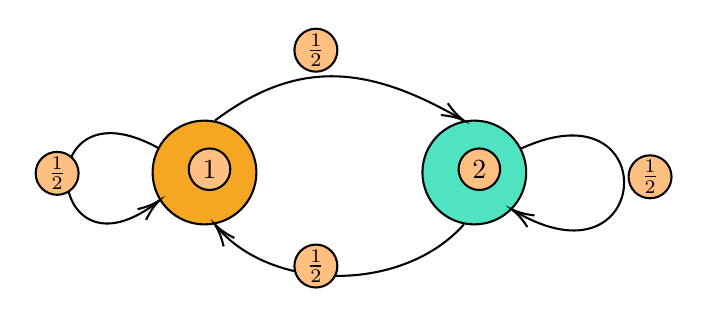
\begin{tikzpicture}[x=0.75pt,y=0.75pt,yscale=-1,xscale=1]
	%uncomment if require: \path (0,300); %set diagram left start at 0, and has height of 300
	
	%Shape: Circle [id:dp10052394937221254] 
	\draw  [fill={rgb, 255:red, 245; green, 166; blue, 35 }  ,fill opacity=1 ] (110,105) .. controls (110,91.19) and (121.19,80) .. (135,80) .. controls (148.81,80) and (160,91.19) .. (160,105) .. controls (160,118.81) and (148.81,130) .. (135,130) .. controls (121.19,130) and (110,118.81) .. (110,105) -- cycle ;
	%Shape: Circle [id:dp9437193586251307] 
	\draw  [fill={rgb, 255:red, 80; green, 227; blue, 194 }  ,fill opacity=1 ] (240,105) .. controls (240,91.19) and (251.19,80) .. (265,80) .. controls (278.81,80) and (290,91.19) .. (290,105) .. controls (290,118.81) and (278.81,130) .. (265,130) .. controls (251.19,130) and (240,118.81) .. (240,105) -- cycle ;
	%Curve Lines [id:da17352138739767575] 
	\draw    (140,80) .. controls (179.6,50.3) and (213.32,53.02) .. (258.62,79.2) ;
	\draw [shift={(260,80)}, rotate = 210.34] [color={rgb, 255:red, 0; green, 0; blue, 0 }  ][line width=0.75]    (10.93,-3.29) .. controls (6.95,-1.4) and (3.31,-0.3) .. (0,0) .. controls (3.31,0.3) and (6.95,1.4) .. (10.93,3.29)   ;
	%Curve Lines [id:da2659131152083798] 
	\draw    (141.59,131.91) .. controls (168.23,162.45) and (230.6,163.07) .. (260,130) ;
	\draw [shift={(140,130)}, rotate = 51.62] [color={rgb, 255:red, 0; green, 0; blue, 0 }  ][line width=0.75]    (10.93,-3.29) .. controls (6.95,-1.4) and (3.31,-0.3) .. (0,0) .. controls (3.31,0.3) and (6.95,1.4) .. (10.93,3.29)   ;
	%Curve Lines [id:da5459168562000609] 
	\draw    (113,93.33) .. controls (50.31,58.59) and (57.92,161.7) .. (112.51,119.07) ;
	\draw [shift={(113.33,118.41)}, rotate = 141.3] [color={rgb, 255:red, 0; green, 0; blue, 0 }  ][line width=0.75]    (10.93,-3.29) .. controls (6.95,-1.4) and (3.31,-0.3) .. (0,0) .. controls (3.31,0.3) and (6.95,1.4) .. (10.93,3.29)   ;
	%Curve Lines [id:da26931738393220694] 
	\draw    (287.67,93.41) .. controls (356.99,61.57) and (351.39,163.71) .. (284.02,123.36) ;
	\draw [shift={(283,122.74)}, rotate = 31.58] [color={rgb, 255:red, 0; green, 0; blue, 0 }  ][line width=0.75]    (10.93,-3.29) .. controls (6.95,-1.4) and (3.31,-0.3) .. (0,0) .. controls (3.31,0.3) and (6.95,1.4) .. (10.93,3.29)   ;
	
	% Text Node
	\draw (130,96) node [anchor=north west][inner sep=0.75pt]   [align=left] {1};
	% Text Node
	\draw (260,96) node [anchor=north west][inner sep=0.75pt]   [align=left] {2};
	% Text Node
	\draw (56.33,97.73) node [anchor=north west][inner sep=0.75pt]   {$\frac{1}{2}$};
	% Text Node
	\draw (342,99.4) node [anchor=north west][inner sep=0.75pt]  {$\frac{1}{2}$};
	% Text Node
	\draw (181,38.4) node [anchor=north west][inner sep=0.75pt]  {$\frac{1}{2}$};
	% Text Node
	\draw (181,142.4) node [anchor=north west][inner sep=0.75pt]   {$\frac{1}{2}$};
	
	
\end{tikzpicture}
\end{figure}\\
	In this example, the state space is $S = \{0,1\}$, and the sample space is
	\[ \Omega = \{ (x_1,x_2,\cdots): x_i \in S \} \]
	which is basically the set of all sequences of one's and zero's. Given this, the random variables $(X_n)_n$ defined t be
	\[  X_n (\omega) = x_n, \]  
	where $\omega \in \Omega$ and $x_n$ is the $n$-th letter in $\omega$. Intuitively speaking, we know that 
	\[  P(1,0) = \prob(X_{n+1} = 1 | X_n = 0) = \frac{1}{2}. \]
	However, here we want to derive that number more explicitly by working directly with the elements of the probability space. First, we need to determine the event associated with $X_{n+1} = 1$. This is the event that has elements where the $n+1$-th position is 1. I.e.
	\[  E = \{  (x_1,x_2, \cdots, x_n, 1, x_{n+2}, \cdots) : x_i \in S\}.  \]
	Similarly, we have
	\[ F = \{ (x_1,x_2, \cdots, x_{n-1},0,x_{n+1},\cdots): x_i \in S \}. \]
	So we have
	\[ \prob(X_{n+1} = 1 | X_n = 0)  = \prob(E|F) = \frac{\prob(E\cap F)}{\prob(F)} =\frac{\prob(E\cap F)}{\prob(F\cap E) + \prob(F\cap E^c)} = \frac{\frac{1}{\abs{\Omega}}}{\frac{1}{\abs{\Omega}} + \frac{1}{\abs{\Omega}}} = \frac{1}{2}. \]
	Note that $\prob(E\cap F) = \frac{1}{\abs{\Omega}}$, since out of many combinations of the sequence of zeros and ones, there is one one sequence whose $n$-th place is 0 and $n+1$-th place is 1. Furthermore, $\prob(F\cap E^c) = \frac{1}{\abs{\Omega}}$ as there is only one string where its $n$-th and $(n+1)$-th string are both zero. 
\end{problem}

\begin{problem}
	In a sequence of independent flips of a fair coin, let N denote the number of flips until there is a run of three consecutive heads. Find
	\begin{enumerate}[(a)]
		\item $\prob(N\leq 8)$,
		\item $\prob(N = 8)$.
	\end{enumerate}
\end{problem}
\begin{solution}
	Let $X_n$ denote the number of consecutive heads at step $n$. For instance for the outcome $\omega \in \Omega$ where $\omega = HTTHTTHHHTTHT\hdots$, $X_2(\omega) = 0$ since the second symbol is $T$ thus there is no consecutive heads. But $X_4(\omega) = 1$, as there is one consecutive heads at step 4. Lastly $X_9(\omega) = 3$, since there is three consecutive heads at step 9. This Markov chain will have the following transition diagram.
	
	\begin{center}
		\begin{tikzpicture}[->,>=stealth',shorten >=1pt,auto,node distance=2.1cm,
			semithick,scale=0.7]
			\tikzstyle{every state}=[circle, draw, fill=orange!50,
			inner sep=0pt, minimum size=15pt]
			
			\node[state] (A1)              {$1$};
			\node[state] (A2) [right of = A1] {$2$};
			\node[state] (A0) [above=of $(A1)!0.5!(A2)$,yshift=-1cm]   {$0$};
			\node[state] (A3) [right of = A2] {$3$};
			
			\path 
			(A0) edge [loop above] node {$0.5$} (A0)
			(A0) edge [bend left] node [sloped,below] {$0.5$} (A1)
			(A1) edge [bend left] node [sloped] {$0.5$} (A0)
			(A2) edge node [above, sloped] {$0.5$} (A0)
			(A1) edge node [below] {$0.5$} (A2)
			(A2) edge node {$0.5$} (A3)
			(A3) edge [loop right] node {$1$} (A3)
			;
			
			%				\path 
			%				(A) edge [loop left] node {$\frac{1}{2}$} (A)
			%				(A) edge [bend left] node {$\frac{1}{2}$} (B)
			%				(B) edge [loop right] node {$\frac{1}{2}$} (B)
			%				(B) edge [bend left] node {$\frac{1}{2}$} (A);
			
		\end{tikzpicture}
	\end{center}
	The transition probabilities are simply computed by the first step argument. For instance, for $P(0,1)$ we have
	\[ \prob_0(X_1 = 1) = \underbrace{\prob_0(X_1 = 1|H)}_{1}\underbrace{\prob_0(H)}_{1/2} + \underbrace{\prob_0(X_1 = 1|T)}_{0}\underbrace{\prob_0(T)}_{1/2}, \]
	where $H$ is the event that the flipped coin is heads and $H^c = T$. The transition matrix for this Markov chain will be
	\[
	M = \begin{pmatrix}
		0.5 & 0.5 & 0 & 0 \\
		0.5 & 0 & 0.5 & 0 \\
		0.5 & 0 & 0 & 0.5 \\
		0 & 0 & 0 & 1 \\
	\end{pmatrix}
	\]
	Since the state $3$ is an absorbing state, then if we get there we will be there for the rest of our life! Thus the probability that the random walker has got there for $N\leq 8$ is simply $(M^8)_{(0,3)}$. Then
	\[ \prob(N\leq 8) = 0.4180. \]
	Now for part (b), the probability that the random walker has arrived at the state 3 right at the step 8, is
	\[ \prob(N = 8) = \prob(N\leq 8) - \prob(N\leq 7) = 0.0508. \]
	
	There is yet another approach that we can compute the probability $\prob(N=8)$. To do this, we need to consider 4 states $S = \set{0,1,2,3,4}$ where the state 4 is of when 3 consecutive heads has occurred at the past. So when the random walker enters the state 3 at some time, it moves to the state $4$ at the next time and remains there forever. The state diagram will be
	
	\begin{center}
		\begin{tikzpicture}[->,>=stealth',shorten >=1pt,auto,node distance=2cm,
			semithick,scale=0.7]
			\tikzstyle{every state}=[circle, draw, fill=orange!50,
			inner sep=0pt, minimum size=15pt]
			
			\node[state] (A1)              {$1$};
			\node[state] (A2) [right of = A1] {$2$};
			\node[state] (A0) [above=of $(A1)!0.5!(A2)$,yshift=-1cm]   {$0$};
			\node[state] (A3) [right of = A2] {$3$};
			\node[state] (A4) [right of = A3] {$4$};
			
			
			\path 
			(A0) edge [loop above] node {$0.5$} (A0)
			(A0) edge [bend left] node [sloped,below] {$0.5$} (A1)
			(A1) edge [bend left] node [sloped] {$0.5$} (A0)
			(A2) edge node [above, sloped] {$0.5$} (A0)
			(A1) edge node [below] {$0.5$} (A2)
			(A2) edge node {$0.5$} (A3)
			(A3) edge node {$1$} (A4)
			(A4) edge [loop right] node {$1$} (A4)
			;
			
			%				\path 
			%				(A) edge [loop left] node {$\frac{1}{2}$} (A)
			%				(A) edge [bend left] node {$\frac{1}{2}$} (B)
			%				(B) edge [loop right] node {$\frac{1}{2}$} (B)
			%				(B) edge [bend left] node {$\frac{1}{2}$} (A);
			
		\end{tikzpicture}
	\end{center}
	Then the transition matrix will be
	\[
	M = \begin{pmatrix}
		0.5 & 0.5 & 0 & 0 & 0 \\
		0.5 & 0 & 0.5 & 0 & 0 \\
		0.5 & 0 & 0 & 0.5 & 0 \\
		0 & 0 & 0 & 0 & 1 \\
		0 & 0 & 0 & 0 & 1
	\end{pmatrix}
	\]
	Then the probability $\prob(N=8) = (M^8)_{(0,3)} = 0.05080.$
\end{solution}


\begin{problem}[Gambler's Ruin]
	Suppose Alice and Bob have in total of $N$ coins. Alice and Bob play a game with a fair coin. When Alice wins, gets a coin from Bop, and vise versa. What is the probability that Alice wins if she starts with $0\leq a \leq N$ coins.
\end{problem}
\begin{solution}
	There are many ways to tackle a probability problem like this and the solution presented here is not the only way to find the solution to this problem. We want to model this with Markov chain whose state space is $\{0,1,2,\cdots,N\}$. Thus $X_n$ represents the fortune of Alice after playing the games for $n$ times. 
	\begin{figure}[h!]
	\centering
	
	
	
	\tikzset{every picture/.style={line width=0.75pt}} %set default line width to 0.75pt        
	
	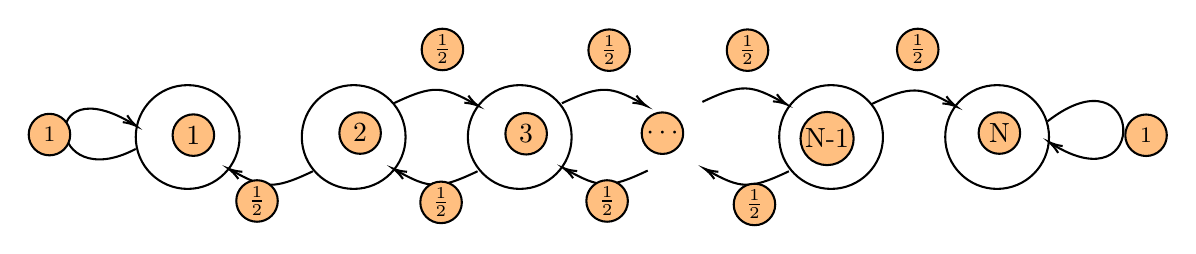
\begin{tikzpicture}[x=0.75pt,y=0.75pt,yscale=-1,xscale=1]
		%uncomment if require: \path (0,300); %set diagram left start at 0, and has height of 300
		
		%Shape: Circle [id:dp09774088338298847] 
		\draw   (100,125) .. controls (100,111.19) and (111.19,100) .. (125,100) .. controls (138.81,100) and (150,111.19) .. (150,125) .. controls (150,138.81) and (138.81,150) .. (125,150) .. controls (111.19,150) and (100,138.81) .. (100,125) -- cycle ;
		%Shape: Circle [id:dp43482816564378113] 
		\draw   (180,125) .. controls (180,111.19) and (191.19,100) .. (205,100) .. controls (218.81,100) and (230,111.19) .. (230,125) .. controls (230,138.81) and (218.81,150) .. (205,150) .. controls (191.19,150) and (180,138.81) .. (180,125) -- cycle ;
		%Shape: Circle [id:dp7628960050576648] 
		\draw   (260,125) .. controls (260,111.19) and (271.19,100) .. (285,100) .. controls (298.81,100) and (310,111.19) .. (310,125) .. controls (310,138.81) and (298.81,150) .. (285,150) .. controls (271.19,150) and (260,138.81) .. (260,125) -- cycle ;
		%Shape: Circle [id:dp3849023603262607] 
		\draw   (410,125) .. controls (410,111.19) and (421.19,100) .. (435,100) .. controls (448.81,100) and (460,111.19) .. (460,125) .. controls (460,138.81) and (448.81,150) .. (435,150) .. controls (421.19,150) and (410,138.81) .. (410,125) -- cycle ;
		%Shape: Circle [id:dp902561209940324] 
		\draw   (490,125) .. controls (490,111.19) and (501.19,100) .. (515,100) .. controls (528.81,100) and (540,111.19) .. (540,125) .. controls (540,138.81) and (528.81,150) .. (515,150) .. controls (501.19,150) and (490,138.81) .. (490,125) -- cycle ;
		%Curve Lines [id:da2277389625716164] 
		\draw    (224.33,108.74) .. controls (243.31,99.74) and (247.7,100.35) .. (263.26,109.02) ;
		\draw [shift={(265,110)}, rotate = 209.42] [color={rgb, 255:red, 0; green, 0; blue, 0 }  ][line width=0.75]    (6.56,-1.97) .. controls (4.17,-0.84) and (1.99,-0.18) .. (0,0) .. controls (1.99,0.18) and (4.17,0.84) .. (6.56,1.97)   ;
		%Curve Lines [id:da8597065575180056] 
		\draw    (305.33,108.74) .. controls (324.31,99.74) and (328.7,100.35) .. (344.26,109.02) ;
		\draw [shift={(346,110)}, rotate = 209.42] [color={rgb, 255:red, 0; green, 0; blue, 0 }  ][line width=0.75]    (6.56,-1.97) .. controls (4.17,-0.84) and (1.99,-0.18) .. (0,0) .. controls (1.99,0.18) and (4.17,0.84) .. (6.56,1.97)   ;
		%Curve Lines [id:da07306821532750352] 
		\draw    (454.67,109.08) .. controls (473.65,100.07) and (478.03,100.69) .. (493.59,109.36) ;
		\draw [shift={(495.33,110.33)}, rotate = 209.42] [color={rgb, 255:red, 0; green, 0; blue, 0 }  ][line width=0.75]    (6.56,-1.97) .. controls (4.17,-0.84) and (1.99,-0.18) .. (0,0) .. controls (1.99,0.18) and (4.17,0.84) .. (6.56,1.97)   ;
		%Shape: Boxed Bezier Curve [id:dp2584084656510479] 
		\draw    (185.33,141.51) .. controls (166.35,150.51) and (161.97,149.9) .. (146.41,141.23) ;
		\draw [shift={(144.67,140.25)}, rotate = 29.42] [color={rgb, 255:red, 0; green, 0; blue, 0 }  ][line width=0.75]    (6.56,-1.97) .. controls (4.17,-0.84) and (1.99,-0.18) .. (0,0) .. controls (1.99,0.18) and (4.17,0.84) .. (6.56,1.97)   ;
		%Shape: Boxed Bezier Curve [id:dp08231579755337615] 
		\draw    (264.67,141.51) .. controls (245.69,150.51) and (241.3,149.9) .. (225.74,141.23) ;
		\draw [shift={(224,140.25)}, rotate = 29.42] [color={rgb, 255:red, 0; green, 0; blue, 0 }  ][line width=0.75]    (6.56,-1.97) .. controls (4.17,-0.84) and (1.99,-0.18) .. (0,0) .. controls (1.99,0.18) and (4.17,0.84) .. (6.56,1.97)   ;
		%Shape: Boxed Bezier Curve [id:dp9912054198682547] 
		\draw    (346.67,141.17) .. controls (327.69,150.18) and (323.3,149.56) .. (307.74,140.89) ;
		\draw [shift={(306,139.92)}, rotate = 29.42] [color={rgb, 255:red, 0; green, 0; blue, 0 }  ][line width=0.75]    (6.56,-1.97) .. controls (4.17,-0.84) and (1.99,-0.18) .. (0,0) .. controls (1.99,0.18) and (4.17,0.84) .. (6.56,1.97)   ;
		%Shape: Boxed Bezier Curve [id:dp49752798194307046] 
		\draw    (414.67,141.51) .. controls (395.69,150.51) and (391.3,149.9) .. (375.74,141.23) ;
		\draw [shift={(374,140.25)}, rotate = 29.42] [color={rgb, 255:red, 0; green, 0; blue, 0 }  ][line width=0.75]    (6.56,-1.97) .. controls (4.17,-0.84) and (1.99,-0.18) .. (0,0) .. controls (1.99,0.18) and (4.17,0.84) .. (6.56,1.97)   ;
		%Curve Lines [id:da6769266285825299] 
		\draw    (373,108.08) .. controls (391.98,99.07) and (396.37,99.69) .. (411.93,108.36) ;
		\draw [shift={(413.67,109.33)}, rotate = 209.42] [color={rgb, 255:red, 0; green, 0; blue, 0 }  ][line width=0.75]    (6.56,-1.97) .. controls (4.17,-0.84) and (1.99,-0.18) .. (0,0) .. controls (1.99,0.18) and (4.17,0.84) .. (6.56,1.97)   ;
		%Curve Lines [id:da5266663507857827] 
		\draw    (539.33,117.41) .. controls (585.53,81.44) and (589.59,158.51) .. (541.47,128.36) ;
		\draw [shift={(540,127.41)}, rotate = 33.33] [color={rgb, 255:red, 0; green, 0; blue, 0 }  ][line width=0.75]    (6.56,-1.97) .. controls (4.17,-0.84) and (1.99,-0.18) .. (0,0) .. controls (1.99,0.18) and (4.17,0.84) .. (6.56,1.97)   ;
		%Curve Lines [id:da13630212552736864] 
		\draw    (100,130.74) .. controls (56.77,153.51) and (52.74,90.36) .. (98.92,118.85) ;
		\draw [shift={(100.33,119.74)}, rotate = 212.76] [color={rgb, 255:red, 0; green, 0; blue, 0 }  ][line width=0.75]    (6.56,-1.97) .. controls (4.17,-0.84) and (1.99,-0.18) .. (0,0) .. controls (1.99,0.18) and (4.17,0.84) .. (6.56,1.97)   ;
		
		% Text Node
		\draw (120.33,116.67) node [anchor=north west][inner sep=0.75pt]   [align=left] {1};
		% Text Node
		\draw (200.67,115.67) node [anchor=north west][inner sep=0.75pt]   [align=left] {2};
		% Text Node
		\draw (280.67,116) node [anchor=north west][inner sep=0.75pt]   [align=left] {3};
		% Text Node
		\draw (423.67,116.33) node [anchor=north west][inner sep=0.75pt]   [align=left] {N-1};
		% Text Node
		\draw (508.67,115.67) node [anchor=north west][inner sep=0.75pt]   [align=left] {N};
		% Text Node
		\draw (151,148.4) node [anchor=north west][inner sep=0.75pt]  [font=\footnotesize]  {$\frac{1}{2}$};
		% Text Node
		\draw (239.67,149.07) node [anchor=north west][inner sep=0.75pt]  [font=\footnotesize]  {$\frac{1}{2}$};
		% Text Node
		\draw (319.67,148.4) node [anchor=north west][inner sep=0.75pt]  [font=\footnotesize]  {$\frac{1}{2}$};
		% Text Node
		\draw (390.67,150.07) node [anchor=north west][inner sep=0.75pt]  [font=\footnotesize]  {$\frac{1}{2}$};
		% Text Node
		\draw (469.33,75.4) node [anchor=north west][inner sep=0.75pt]  [font=\footnotesize]  {$\frac{1}{2}$};
		% Text Node
		\draw (387.33,75.73) node [anchor=north west][inner sep=0.75pt]  [font=\footnotesize]  {$\frac{1}{2}$};
		% Text Node
		\draw (320.67,75.73) node [anchor=north west][inner sep=0.75pt]  [font=\footnotesize]  {$\frac{1}{2}$};
		% Text Node
		\draw (240.33,75.4) node [anchor=north west][inner sep=0.75pt]  [font=\footnotesize]  {$\frac{1}{2}$};
		% Text Node
		\draw (579.33,116.73) node [anchor=north west][inner sep=0.75pt]  [font=\footnotesize]  {$1$};
		% Text Node
		\draw (51,116.4) node [anchor=north west][inner sep=0.75pt]  [font=\footnotesize]  {$1$};
		% Text Node
		\draw (346.33,115.73) node [anchor=north west][inner sep=0.75pt]    {$\cdots $};
		
		
	\end{tikzpicture}
\end{figure} \\
	Let $p_a$ be the probability of Alice wining if she starts with $a$ coins. First, observe that $p_0 = 0$ and $p_N= 1$. Let $E$ denote that event of Alice wining the whole game. Also, let $F_1$ be the event in which she looses the first game and $F_2$ the event in which she wins the first game. Then
	\[ p_a = \prob_a(E) =  \underbrace{\prob_a(E | F_1)}_{\prob(E|F_1,X_0=a)} \prob(F_1) + \underbrace{\prob_a(E|F_1^c)}_{\prob(E|F_1^c,X_0=a)}\prob(F_1^c) \]
	(note that this identity is actually true for any set $F_1$, but here $F_1$ is the specific event explained above). The probability that she looses or wins the first game is $\frac{1}{2}$. Also, observe that $\prob_a(E|F_1) = p_{a+1}$ (since if she wins the first game she will have one more coin) and $\prob_a(E|F_1^c) = p_{a-1}$. Thus 
	\[ p_a = \frac{1}{2}p_{a+1} + \frac{1}{2}p_{a-1}. \]
	Now we can solve this recurrent equation with the characterization polynomial which is $2 = X + 1/X$ or $X^2 - 2X + 1 = (X-1)^2 = 0$. Thus the characteristic polynomial has a double root. Thus 
	\[ p_a = (Aa + B)(1)^a = Aa + B. \]
	Since $p_0 = 0,\ p_N =1$, then it turns out that
	\[ p_a = \frac{a}{N}. \]
\end{solution}

\begin{problem}[Gambler's Ruin with Draw]
	Let Alice and Bob play Rock-Paper-Scissors. If Alice and Bob has a total of $N$ coins, and at each play, the winner gets one coin from the loser, what is the probability that Alice will win the game if he starts with $a$ coins. When they draw, then they repeat the game (or equivalently, they play another game without any coins exchange).
\end{problem}
\begin{solution}
	We need to do a first step analysis similar to what we did before. Let $E$ be the event that Alice wins the whole game, and the event $F=F_{-1}\cup F_0 \cup F_1$ where
	\begin{quote}
		$F_{-1}$: Alice loses the first game,\\
		$F_0$: Alice draws the first game,\\
		$F_1$: Alice wins the first game.
	\end{quote}
	It is clear that $\prob(F) = 1$, since the components are mutually disjoint. Thus $E\cap F_{-1},\ E\cap F_0,\ E\cap F_1$ are also mutually disjoints where. Thus we can write
	\[\prob_a(E) = \prob_a(E\cap F_{-1}) + \prob_a(E\cap F_0) + \prob_a(E\cap F_1)
	= \prob_a(E|F_{-1})\prob_a(F_{-1}) + \prob_a(E|F_0)\prob_a(F_0) + \prob_a(E|F_1)\prob_a(F_1).
	\]
	Since the game is fair we know
	\[ \prob_a(F_{-1}) = \prob_a(F_0) = \prob_a(F_1) = \frac{1}{3}.  \]
	Furthermore, we know
	\[ \prob_a(E|F_{-1}) = p_{a-1}, \qquad \prob_a(E|F_0) = p_a, \qquad \prob_a(E|F_1) = p_{a+1}. \]
	Thus the first step analysis will lead to the following identity.
	\[  \prob_a(E) = p_a = \frac{1}{3} ( p_{a-1} + p_{a} + p_{a+1}),\]
	which after simplification becomes
	\[ 2p_a = p_{a-1} + p_{a+1}, \]
	which is the same recursive formula we got in the previous example. So the possibility of the draw, will not change the behaviour of the system.
\end{solution}

\begin{problem}
	Consider the a simple random walker on the following graph. Let $B = \{ T_{\tilde{x}} < T_{\set{\tilde{z},\tilde{y}}} \}$. Compute the probability $\prob_0(B)$.
	
	\begin{center}
		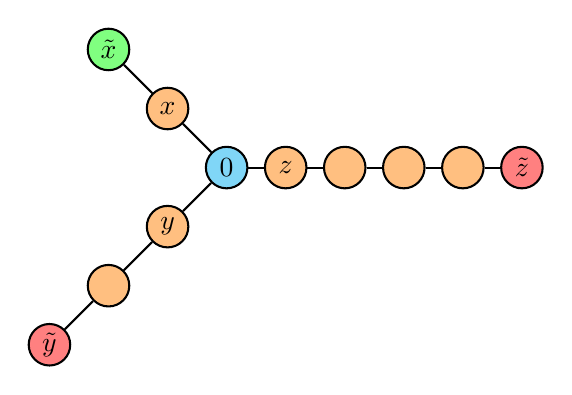
\begin{tikzpicture}[scale=1.5, every node/.style={circle, draw}]
			\tikzstyle{every node}=[circle, draw, fill=white,
			inner sep=0pt, minimum width=15pt]
			
			\node[fill=cyan!50] (a) at (0,0) {0};
			\node[fill=orange!50] (z1) at (1/2,0) {$z$};
			\node[fill=orange!50] (z2) at (2/2,0) {};
			\node[fill=orange!50] (z3) at (3/2,0) {\ };
			\node[fill=orange!50] (z4) at (4/2,0) {\ };
			\node[fill=red!50] (ze) at (5/2,0) {$\tilde{z}$};
			
			\node[fill=orange!50] (x1) at (-1/2,1/2) {$x$};
			\node[fill=green!50] (xe) at (-1,1) {$\tilde{x}$};
			
			\node[fill=orange!50] (y1) at (-1/2,-1/2) {$y$};
			\node[fill=orange!50] (y2) at (-2/2,-2/2) {};
			\node[fill=red!50] (ye) at (-3/2,-3/2) {$\tilde{y}$};
			
			
			\draw (a) -- (z1);
			\draw (z1) -- (z2);
			\draw (z2) -- (z3);
			\draw (z3) -- (z4);
			\draw (z4) -- (ze);
			
			\draw (a) -- (y1);
			\draw (y1) -- (y2);
			\draw (y2) -- (ye);
			
			\draw (a) -- (x1);
			\draw (x1) -- (xe);
			
		\end{tikzpicture}
	\end{center}
\end{problem}
\begin{solution}
	This problem is simply asking what is the probability that we hit $\tilde{x}$ state before hitting any of $\tilde{y}$ or $\tilde{z}$ states, given the fact that the random walker starts from the state $0$. To keep unnecessary details out of the way, we have only labeled the vertices that we will use in our analysis. We will have the following notation to simplify the solution
	\[ p_v = \prob_v(B), \]
	where $v$ is any vertex in the graph. Note that starting at 0, i.e. $X_0=0$, then going to any of the states $x,y$, or $z$, are mutually disjoint events, and the probability of the union of these events is one. With our first time step analysis (see \autoref{prop:FirstTimeStepArgument}) we can write
	\[ \prob_0(B) = \frac{1}{3} ( p_x + p_y + p_z). \]
	Now we need to analyze each of terms in the RHS. Let's start with $p_z$. Consider two events $\{ T_0 < T_{\tilde{z}}  \}$ and $\{ T_0 > T_{\tilde{z}}  \}$, where the first time is the event where the random walker hits the $0$ state before hitting the $\tilde{z}$ step first, and the second one is the vice versa. These two events are disjoint and the probability of the union is 1. Thus we write the conditional expansion of $p_z$ based on these events
	\[ p_z = \prob_z(B) = \prob_z(B|T_0 < T_{\tilde{z}})\prob_z(T_0 < T_{\tilde{z}}) + \prob_z(B|T_0 > T_{\tilde{z}})\prob_z(T_0 > T_{\tilde{z}}). \]
	We know that $\prob_z(B|T_0 > T_{\tilde{z}}) = \prob(B|X_0=z,X_i=\tilde{z})$ for some $i > 0$. From Markov property it follows that 
	\[ \prob(B|X_0=z,X_i=\tilde{z}) = \prob(B|X_i=\tilde{z}) = \prob(B|X_0 = \tilde{z})  = p_{\tilde{z}}.\]
	Also $\prob_z(B|T_0<T_{\tilde{z}}) = \prob_0(B) = p_0$ by the Markov property. Lastly, $\prob_z(T_0<T_{\tilde{z}})$ is determined by the Gambler's ruin method we say before, which is basically
	\[ \prob_z(T_0 < T_{\tilde{z}}) = \frac{5}{4}, \qquad \prob_z(T_0>T_{\tilde{z}}) = \frac{1}{5}. \]
	By doing the same kind of analysis for $p_x$ as well as $p_y$ we will get
	\[ p_z = \frac{4}{5}p_0 , \qquad p_y = \frac{2}{3}p_0, \qquad p_x =\frac{1}{2}p_0 + \frac{1}{2}. \]
	Now by substituting in the identity we got from the first time step argument, we can fine that 
	\[ p_0 = \frac{15}{31}, \]
	And this completes our solution for the problem.
\end{solution}

\begin{problem}
	Consider the graph $\gamma=  (V,E)$ drawn below. Set $Z = \{2,3\}$, and $W = \set{6,9}$. Compute $\prob_0(T_Z<T_W)$. In colors: we start at blue, win if we reach green, and lose of we reach red.
	
	\begin{center}
		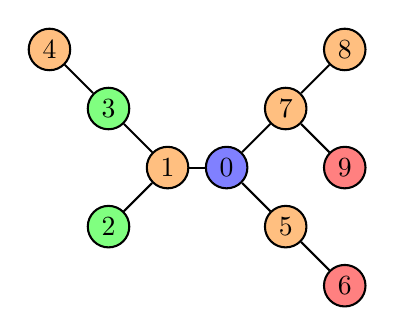
\begin{tikzpicture}[scale=1.5, every node/.style={circle, draw}]
			\tikzstyle{every node}=[circle, draw, fill=orange!50,
			inner sep=0pt, minimum width=15pt]
			
			\node[fill=blue!50] (n0) at (1/2,0) {0};
			\node (n1) at (0/2,0) {1};
			\node[fill=green!50] (n2) at (-1/2,-1/2) {2};
			\node[fill=green!50] (n3) at (-1/2,1/2) {3};
			\node (n4) at (-2/2,2/2) {4};
			\node (n5) at (2/2,-1/2) {5};
			\node[fill=red!50] (n6) at (3/2,-2/2) {6};
			\node (n7) at (2/2,1/2) {7};
			\node (n8) at (3/2,2/2) {8};
			\node[fill=red!50] (n9) at (3/2,0/2) {9};
			
			
			\draw (n0) -- (n1);
			\draw (n1) -- (n2);
			\draw (n1) -- (n3);
			\draw (n3) -- (n4);
			\draw (n0) -- (n7);
			\draw (n0) -- (n5);
			\draw (n5) -- (n6);
			\draw (n7) -- (n9);
			\draw (n7) -- (n8);
			
		\end{tikzpicture}
	\end{center}
\end{problem}

\begin{solution}
	As always, we start with our powerful tool in hand, which is the first step argument (which is basically a special form of the more general conditional expansion). We start with first step argument at state $0$. We will get
	\[ \prob_0(B) = \frac{1}{3} (\prob_1(B) + \prob_7(B) + \prob_5(B) ), \]
	and now we need to analyze each of the terms in the right hand side. We start with $\prob_5(B)$ which is the most straight forward one. As we saw in the last example, we can analyze this state with a conditional expansion on the two disjoint events, whose union probability is 1. Let those two events be $\set{T_6 < T_0}$ (where the random walker hits the state $6$ before hitting the state $0$), and $\set{T_6 > T_0}$, where the random walker hits the state $0$ before hitting the state $6$. Thus the expansion will be
	\[ \prob_5(B) = \prob_5(B|T_6 < T_0) \prob_5(T_6 < T_0) + \prob_5(B|T_6 > T_0)\prob_5(T_6 > T_0). \]
	We know that if we hit the state $6$ before $0$, we have no chance to hit any of the green states (we will lose). Thus
	\[ \prob_5(B|T_6<T_0) = 0. \]
	And from the Gambler's ruin we know that $\prob_5(T_6>T_0) = 1/2$, and from the Markov property we know that $\prob_5(B|T_6>T_0) = \prob_0(B)$, because the conditional probability $\prob_5(B|T_6>T_0)$ is basically stating what is the probability of $B$ happening, if we start from $5$ and $X_i = 0$ for some $i$ in the future. Thus 
	\[ \prob_5(B) = \frac{\prob_0(B)}{2}. \]
	Now, we need to analyze the term $\prob_1(B)$. Again, at this step, we do another first step analysis.
	\[  \prob_1(B) = \frac{1}{3} (\underbrace{\prob_3(B)}_{=1} + \underbrace{\prob_2(B)}_{=1} +\prob_0(B)) = \frac{2+\prob_0(B)}{3}. \]
	Note that from the assumption, we know that if we reach any of green states, then we are declared winner, that is why we have $\prob_3(B) = \prob_2(B) = 1$. Now it only remains to analyze the term $\prob_7(B)$. Again, similar to the case above, we do a first time step argument
	\[ \prob_7(B) = \frac{1}{3} ( \prob_0(B) + \underbrace{\prob_8(B)}_{=\prob_7(B)} + \underbrace{\prob_9(B)}_{=0} ) \implies \prob_7(B) = \frac{\prob_0(B)}{2}.\]
	Note that $\prob_8(B) = \prob_7(B)$ by a first stem analysis when starting at the state $8$. Putting all of these terms back to the original identity we derived the first, we can conclude that 
	\[ p_0 = \prob_0(B) = \frac{2}{5}. \]
\end{solution}


\begin{problem}
	The French roulette game has slots numbered from 0 to 36. The slot 0 is green, Among the slots from 1 to 36, 18 are black and 18 are red. Alex goes to a casino to play roulette. Their strategy is to always bet ``red''. They start with 50 coins, play 1 coin each turn, and stop when reaching 100 or getting broke.
	\begin{enumerate}[(a)]
		\item What is the probability that Alex reaches 100?
		\item How many coins should Alex start with to have about $50\%$ chance to reach 100?
	\end{enumerate}
\end{problem}

\begin{solution}
	\begin{enumerate}[(a)]
		\item
		Let $B$ be the event $B = \set{T_{100} < T_0}$ and we are looking for $\prob_a(B)$ where $0 \leq a \leq 100$ and indicates the number of coins we are starting with. First observe that
		\begin{itemize}
			\item $p_0 = 0$: Since if we start with zero coins we are already broken and the game is over.
			\item $p_{100} = 1$: Since if we start with 100 coins then we won the game and the game is finished.
		\end{itemize}
		To compute the probability for intermediate values of $a$, we do the first step argument. Let $WF$ be the event where Alex wins the first bet, and $LF$ the event where Alex loses the first bet. Then we can write
		\[ p_a = \prob_a(B) = \prob_a(B|WF)\prob_a(WF) + \prob_a(B|LF) \prob_a(LF). \]
		Since there are 18 red spots, then the chance to win the first bet is
		\[ \prob_a(WF) = \frac{18}{37}. \]
		and since there are 19 non-red spots in total, then the chance to win is
		\[ \prob_a(LF)  = \frac{19}{37}.\]
		Also, from Markov property, we know that
		\[ \prob_a(B|WF)= p_{a+1}, \qquad \prob_a(B|LF)=p_a. \]
		Thus the first step argument formula will be
		\[  p_a = \frac{18}{37}p_{a+1} + \frac{19}{37}p_{a-1} \implies \boxed{37p_a = 18p_{a+1} + 19p_{a-1}}. \]
		The characteristic equation for the recursive equation is
		\[ 37 = 18 x + \frac{19}{x} \implies \boxed{18x^2 - 37x + 19 = 0}. \]
		We can write it as $(x-1)(18x-19) = 0$. Thus the roots will be
		\[ r_1 = 1, \qquad r_2 = \frac{19}{18}. \]
		So
		\[ p_a = A + Br_2^a. \]
		To fine $A$ and $B$ we use the fact $p_0 = 0$, and $p_{100} = 1$. Then $A = -B$, and $A = 1/(1-r_2^{100})$. Thus
		\[ \boxed{p_a = \frac{1-r_2^a}{1-r_2^{100}}}.  \]
		
		\item  We basically need to compute find $a$ for which $p_a = 1/2$. Thus we need to solve for $a$
		\[ \frac{1-r_2^a}{1-r_2^{100}} = \frac{1}{2}. \]
		After some algebra we will find
		\[  \boxed{a = \frac{\ln(\frac{1+r_2^{100}}{2})}{\ln(r_2)} \approx 87.26}.  \]
		Thus we need to start with at least 88 coins to have a $50\%$ chance of winning.
	\end{enumerate}
	\qed
\end{solution}


\begin{problem}
	There are 6 coins on a table, each showing heads (H) or tails (T). In each step we 
	\begin{itemize}
		\item Select uniformly one of the coins. 
		\item If it is heads, toss it and replace on the table (with random side).
		\item If it sis tails, toss it. If it comes up heads, leave it at that. If it comes up tails, toss it a second time, and leave the result as it is.
		Let $X_n$ be the number of heads showing after $n$ such steps. Answer the following questions
		\begin{enumerate}[(a)]
			\item Determine the transition probabilities for this Markov chain.
			\item Draw the transition diagram and write the transition matrix.
			\item What is $\prob(X_2 = 4| X_0=5)$?
		\end{enumerate}
	\end{itemize}
\end{problem}
\begin{solution}
	\begin{enumerate}[(a)]
		\item To compute the transition probabilities, we need to perform the first step analysis. Let the events \[I = \set{X_1 = a+1},\qquad S = \set{X_1 = a},\qquad D = \set{X_1 = a-1},\]
		where $0 \leq a \leq 6$ is the number of heads. So to compute the transition probabilities, we need to compute
		\[ P(a,a+1) = \prob_a(I), \qquad P(a,a) = \prob_a(S), \qquad P(a,a-1) = \prob_a(D). \]
		We start with $\prob_a(I)$. Let $ST$ be the event where the selected coin is tails, and $SH$ be the event where the selected coin is heads. These two events are disjoint and the probability of their union is 1, thus
		\[ \prob_a(I) = \underbrace{\prob_a(I|SH)}_{\text{see Eq (2.I.1)}}\underbrace{\prob_a(SH)}_{\frac{a}{6}} + \underbrace{\prob_a(I|ST)}_{\text{see Eq (2.I.2)}}\underbrace{\prob_a(ST)}_{\frac{6-a}{6}}. \tag{2.I}\]
		Note that if we start with $a$ coins heads, then the chance we choose a random coin from the table and find it heads is $\frac{a}{6}$, hence $\prob_a(SH) = \frac{a}{6}$, and $\prob_a(ST) = \frac{6-a}{6}$. Now we need to expand the remaining terms with appropriate conditioning. Let $TT$ be the event where we toss a coin and find it tails and $TH$ be the event where we toss a coin and find it heads. Thus we can write
		\[ \prob_a(I|SH) = \underbrace{\prob_a(I|SH,TH)}_{0}\underbrace{\prob_a(TS)}_\frac{1}{2} + \underbrace{\prob_a(I|SH,TT)}_{0}\underbrace{\prob_a(TT)}_\frac{1}{2}. \tag{2.I.1}  \]
		Note that $\prob_a(TT) = \prob_a(TH) = \frac{1}{2}$, since the coin tossing is fair. Also, note that $\prob_a(I|SH,TH)=\prob_a(I|SH,TT)=0$ since if we select a heads, and then toss it, finding it either heads or tails will not increase the total number of heads on the table. Similarly, for the other term in $(2.1)$ we have
		\[ \prob_a(I|ST) = \underbrace{\prob_a(I|ST,TH)}_{1}\underbrace{\prob_a(TH)}_{\frac{1}{2}} + \underbrace{\prob_a(I|ST,TT)}_\text{see Eq (2.I.3)}\underbrace{\prob_a(TT)}_{\frac{1}{2}}. \tag{2.I.2} \]
		Now we need to expand the remaining terms in the equation above.
		\[ \prob_a(I|ST,TT) = \underbrace{\prob_a(I|ST,TT,TH)}_{1}\prob_a(TH) + \underbrace{\prob_a(I|ST,TT,TT)}_{0}\prob_a(TT) = \frac{1}{2}. \tag{2.I.3}  \]
		Putting all together we can write
		\[ \boxed{P(a,a+1) = \prob_a(I) = \frac{6-a}{8}}. \]
		Similarly, we can compute other transition probabilities. For instance for $\prob_a(S)$ we can write
		\[ \prob_a(S) = \underbrace{\prob_a(S|SH)}_{\text{see Eq (2.S.1)}}\underbrace{\prob_a(SH)}_{\frac{a}{6}} + \underbrace{\prob_a(S|ST)}_{\text{see Eq (2.S.2)}}\underbrace{\prob_a(ST)}_{\frac{6-a}{6}}. \tag{2.S}\]
		and for the remaining terms we can write
		\[ \prob_a(S|SH) = \underbrace{\prob_a(S|SH,TH)}_{1}\underbrace{\prob_a(TS)}_\frac{1}{2} + \underbrace{\prob_a(S|SH,TT)}_{0}\underbrace{\prob_a(TT)}_\frac{1}{2}, \tag{2.S.1}  \]
		and
		\[ \prob_a(S|ST) = \underbrace{\prob_a(S|ST,TH)}_{0}\underbrace{\prob_a(TH)}_{\frac{1}{2}} + \underbrace{\prob_a(S|ST,TT)}_\text{see Eq (2.S.3)}\underbrace{\prob_a(TT)}_{\frac{1}{2}}. \tag{2.S.2} \]
		And for the remaining term above
		\[ \prob_a(S|ST,TT) = \underbrace{\prob_a(S|ST,TT,TH)}_{0}\prob_a(TH) + \underbrace{\prob_a(S|ST,TT,TT)}_{1}\prob_a(TT) = \frac{1}{2}. \tag{2.S.3}  \]
		and by putting all together we will get
		\[\boxed{ P(a,a) =  \prob_a(S) = \frac{6+a}{24}}. \]
		Finally, since $\prob_a(I\cup S \cup D) = 1$, and $I,S,D$ are mutually disjoint, we can write 
		\[ \prob_a(D) = 1 - (\prob_a(I) + \prob_a(S)), \] 
		hence
		\[ \boxed{P(a,a-1) = \prob_a(D) = \frac{a}{12}}. \]
		so the transition probabilities are as calculated.
		
		\item The transition diagram is plotted below. 
		
		\begin{center}
			\begin{tikzpicture}[->,>=stealth',shorten >=1pt,auto,node distance=1.9cm,
				semithick,scale=0.4]
				\tikzstyle{every state}=[circle, draw, fill=orange!50,
				inner sep=0pt, minimum width=10pt]
				
				\node[state] (A)              {$0$};
				\node[state]         (B) [right of=A] {$1$};
				\node[state]         (C) [right of=B] {$2$};
				\node[state]         (D) [right of=C] {$3$};
				\node[state]         (E) [right of=D] {$4$};
				\node[state]         (F) [right of=E] {$5$};
				\node[state]         (G) [right of=F] {$6$};
				
				\path (A) edge [bend left] node {$p_{01}$} (B)
				(B) edge [bend left] node {$p_{10}$} (A)
				(A) edge [loop left] node {$p_{00}$} (A)
				
				(B) edge [bend left] node {$p_{12}$} (C)
				(B) edge [loop above] node {$p_{11}$} (C)
				(C) edge [bend left] node {$p_{21}$} (B)
				
				(C) edge [bend left] node {$p_{23}$} (D)
				(C) edge [loop below] node {$p_{22}$} (D)
				(D) edge [bend left] node {$p_{32}$} (C)
				
				(D) edge [bend left] node {$p_{34}$} (E)
				(D) edge [loop above] node {$p_{33}$} (E)
				(E) edge [bend left] node {$p_{43}$} (D)
				
				(E) edge [bend left] node {$p_{45}$} (F)
				(E) edge [loop below] node {$p_{44}$} (E)
				(F) edge [bend left] node {$p_{54}$} (E)
				
				(F) edge [bend left] node {$p_{56}$} (G)
				(F) edge [loop above] node {$p_{55}$} (E)
				(G) edge [bend left] node {$p_{65}$} (F)
				(G) edge [loop right] node {$p_{66}$} (G);
			\end{tikzpicture}
		\end{center}
		And the transition matrix is
		\[  M =
		\begin{pmatrix}
			1/4 & 3/4 & 0 & 0 & 0 & 0 & 0 \\
			1/12 & 7/24 & 5/8 & 0 & 0 & 0 & 0 \\
			0 & 1/6 & 1/3 & 1/2 & 0 & 0 & 0 \\
			0 & 0 & 1/4 & 3/8 & 3/8 & 0 & 0 \\
			0 & 0 & 0 & 1/3 & 5/12 & 1/4 & 0 \\
			0 & 0 & 0 & 0 & 5/12 & 11/24 & 1/8 \\
			0 & 0 & 0 & 0 & 0 & 1/2 & 1/2
		\end{pmatrix}
		\]
		
		\item $\prob(X_2 = 4|X_0=5)$ is the second transition probability $P_2(5,4)$. To compute this, we need to fine the element in the 6-th row and 5-th column in the $M^2$ matrix, which is basically the inner product between the vectors formed by the 6-th row and the 5-th column.
		\[ P_2(5,4) = (\frac{5}{12})^2 + \frac{11}{24}\cdot\frac{5}{12} = \frac{35}{96} \]
		which after simplification becomes
		\[ \boxed{P_2(5,4) = \frac{35}{96}}. \]
		\qed
		
	\end{enumerate}
\end{solution}



\begin{problem}
	A clock is broken. It has only one hand which moves every hour either clockwise with probability 1/2 or counter-clockwise with probability 1/2 (the numbers are from 0 to 11 and the hand moves by one full hour when it moves). Assume it starts at 0. What is the probability that it reaches 7 before coming back to 0 for the first time?
\end{problem}
\begin{solution}
	First, let's draw the graph representing the state space of the random variable of interest.
	\begin{center}
		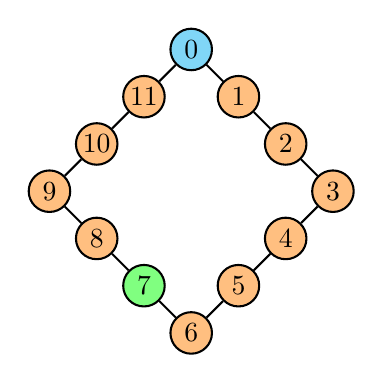
\begin{tikzpicture}[scale=0.6, every node/.style={circle, draw}]
			\tikzstyle{every node}=[circle, draw, fill=orange!50,
			inner sep=0pt, minimum width=15pt]
			
			
			\node[fill=cyan!50] (n0) at (0,3) {0};
			\node (n1) at (1,2) {1};
			\node (n2) at (2,1) {2};
			\node (n3) at (3,0) {3};
			\node (n4) at (2,-1) {4};
			\node (n5) at (1,-2) {5};
			\node (n6) at (0,-3) {6};
			
			\node (n11) at (-1,2) {11};
			\node (n10) at (-2,1) {10};
			\node (n9) at (-3,0) {9};
			\node (n8) at (-2,-1) {8};
			\node[fill=green!50] (n7) at (-1,-2) {7};
			
			
			\draw (n0) -- (n1);
			\draw (n1) -- (n2);
			\draw (n2) -- (n3);
			\draw (n3) -- (n4);
			\draw (n4) -- (n5);
			\draw (n5) -- (n6);
			\draw (n6) -- (n7);
			\draw (n7) -- (n8);
			\draw (n8) -- (n9);
			\draw (n9) -- (n10);
			\draw (n10) -- (n11);
			\draw (n11) -- (n0);
			
		\end{tikzpicture}
	\end{center}
	
	Define the event $B$ be $B = \set{T^+_0 > T_7}$. We are interested in finding $\prob_0(B)$. Now we can perform the first step argument as follows
	\[ p_0 = \frac{1}{2}(p_1 + p_{11}). \tag{3.1} \]
	Then we analyze each term in the right hand side of the equation above. For $p_1$ we have
	\[ \prob_1(B) = \underbrace{\prob_1(B|T_0>T_7)}_{1}\underbrace{\prob_1(T_0>T_7)}_{1/5} + \underbrace{\prob_1(B|T_0<T_7)}_{0}\underbrace{\prob_1(T_0<T_7)}_{6/7} = \frac{1}{5}. \]
	Note that $\prob_1(B|T_0>T_7)=1$ since it literally means the random walker reaches 7 before 0. Also $\prob_1(B|T_0<T_7)=0$ since the event $B$ is conditioned on reaching 0 before 7, which is clearly 0. The term $\prob_1(T_0>T_7)$ is computed using the Gambler's ruin analysis. Similarly, for the $p_{11}$ term we have
	\[ \prob_{11}(B) = \underbrace{\prob_{11}(B|T_0>T_7)}_{1}\underbrace{\prob_{11}(T_0>T_7)}_{1/7} + \underbrace{\prob_{11}(B|T_0<T_7)}_{0}\prob_{11}(T_0<T_7) = \frac{1}{7}. \]
	The rationale behind the values of the terms are the same as the ones discussed above. Now we can substitute everything in $(3.1)$
	\[ \boxed{p_0 = \frac{1}{2} (\frac{12}{35}) = \frac{6}{35}}. \]
	
\end{solution}

\begin{problem}
	The Fibonacci sequence is the sequence $(F_n)_{n\geq0}$ defined by $F_0 = 0, F_1=1$ and 
	\[ F_{n+2} = F_{n+1} + F_n \quad \text{for } n\geq 0.  \]
	Find a general formula for $F_n$
\end{problem}
\begin{solution}
	First, we construct the characteristic polynomial of the sequence. From the recursive formula we can write
	\[ X^2 = X + 1 \implies \boxed{X^2 - X - 1 = 0}. \]
	The roots of the equation is 
	\[ r_1, r_2 = \frac{1 \pm \sqrt{5}}{2}. \]
	Now the general formula will be
	\[ F_n = Ar_1^n + Br_2^n. \] 
	To find the coefficients, we utilize the first two terms 
	\[ 0 = A + B, \qquad 1 = \frac{1}{2}(A+B) + \frac{\sqrt{5}}{2}(A-B). \]
	This system of equations implies that
	\[ A = \frac{1}{\sqrt{5}}, \qquad B=\frac{-1}{\sqrt{5}}.  \]
	Thus the general formula will be
	\[ \boxed{F_n = \frac{1}{\sqrt{5}}((\frac{1+\sqrt{5}}{2})^n - \frac{1-\sqrt{5}}{2})^n)}. \]
	
	\qed
	
\end{solution}


\begin{problem}
	Let $(X_n)$ be the simple random walk on the following graph. Compute $\prob_0(T_3<T_7)$.
	
	\begin{center}
		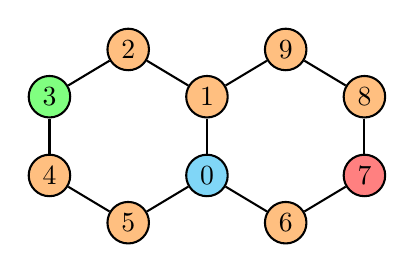
\begin{tikzpicture}[scale=1, every node/.style={circle, draw}]
			\tikzstyle{every node}=[circle, draw, fill=orange!50,
			inner sep=0pt, minimum width=15]
			
			
			\node[fill=cyan!50] (n0) at (0,0) {0};
			\node (n1) at (0,1) {1};
			\node (n2) at (-1,1.6) {2};
			\node[fill=green!50] (n3) at (-2,1) {3};
			\node (n4) at (-2,0) {4};
			\node (n5) at (-1,-0.6) {5};
			\node (n9) at (1,1.6) {9};
			\node (n8) at (2,1) {8};
			\node[fill=red!50] (n7) at (2,0) {7};
			\node (n6) at (1,-0.6) {6};
			
			\draw (n0) -- (n1);
			\draw (n1) -- (n2);
			\draw (n2) -- (n3);
			\draw (n3) -- (n4);
			\draw (n4) -- (n5);
			\draw (n5) -- (n0);
			\draw (n0) -- (n6);
			\draw (n6) -- (n7);
			\draw (n7) -- (n8);
			\draw (n8) -- (n9);
			\draw (n9) -- (n1);
			
			
		\end{tikzpicture}
	\end{center}
\end{problem}
\begin{solution}
	For a much more simpler solution, let's define the two following notations
	\[ B = \{T_3 < T_7\}, \qquad p_v = \prob_v(B). \]
	Then, by first step argument at state $0$, we can write
	\[ p_0 = \frac{1}{3} (p_5 + p_6 + p_1).  \tag{5.1}\]
	Now we need to evaluate each of the terms in the right hand side. We start with $p_5$.
	\[ p_5 = \prob_5(B) = \underbrace{\prob_5(B|T_3<T_0)}_{1}\underbrace{\prob_5(T_3<T_0)}_{1/3} + \underbrace{\prob_5(B|T_3>T_0)}_{p_0}\underbrace{\prob_5(T_3>T_0)}_{2/3} = \frac{1}{3} + \frac{2}{3}p_0. \]
	note that $\prob_5(B|T_3<T_0) = 1$, since if we get to state 3, before getting to state 0, then it means that we have reached the state 3 before reaching the state 7, thus the event $B$ occurs with probability 1. Also $\prob_5(T_3<T_0) = 1/3$ from the Gambler's ruin. Furthermore $\prob_5(B|T_3>T_0) = p_0$ by using the Markov property, and finally $\prob_5(T_3>T_0) = 2/3$ by the Gambler's ruin. \\
	Now, we need to evaluate the term $p_6$. To analyze this term, we will do a first step argument starting at this point
	\[ p_6 = \prob_6(B) = \frac{1}{2}(\underbrace{p_7}_{0} + p_0) = \frac{p_0}{2}. \]
	Note that $p_7 = 0$, since then the event $B$ has not occurred. \\
	Finally, we need to analyze the term $p_1$. Again, by first step argument on this state we have
	\[ p_1 = \frac{1}{3}(p_0 + p_9 + p_2). \]	
	By doing a analysis on $p_9$ similar to the one we did for 5, we can write
	\[ p_9 = \prob_9(B)= \underbrace{\prob_9(B|T_7<T_1)}_{0}\prob_9(T_7<T_1) + \underbrace{\prob_9(B|T_7>T_1)}_{p_1}\underbrace{\prob_9(T_7>T_1)}_{2/3} = \frac{2}{3}p_1. \]
	The rationale behind the values for each term in the equation above, is exactly the same as in analyzing the terms of $p_5$.\\
	Now, we analyze the term $p_2$ by performing another first step analysis, similar to the one we did for state 6.
	\[ p_2 = \frac{1}{2}(\underbrace{p_3}_1 + p_1) = \frac{1}{2}(1+p_1). \]
	Now we can calculate $p_1$ in terms of $p_0$ which turns out to be
	\[ p_1 = \frac{6}{11}p_0 + \frac{3}{11}.  \]
	Now we insert all of the terms in the equation $(5.1)$ to get
	\begin{align*}
		&3p_0 = \frac{1}{3}+\frac{2}{3}p_0 + \frac{1}{2}p_0 + \frac{6}{11}p_0 + \frac{3}{11} \\ 
		&\implies 3p_0 - \frac{113}{66}p_0 = \frac{40}{33} \\
		&\implies p_0 = \frac{66}{85}\cdot\frac{40}{33} = \frac{16}{17}\\
		&\implies \boxed{p_0 = \frac{16}{17}}.
	\end{align*}
	
	
	\qed
	
\end{solution}


\begin{problem}
	Consider the Markov chain on the state space $S = \set{1,2,\cdots,9}$ which has the following transition diagram.
	
	\begin{center}
		\begin{tikzpicture}[->,>=stealth',shorten >=1pt,auto,node distance=2.8cm,
			semithick,scale=1]
			\tikzstyle{every state}=[circle, draw, fill=orange!50,
			inner sep=1pt, minimum size=20pt]
			
			\node[state] 		 (n1)              {$1$};
			\node[state] 		 (n2) [left of=n1] {$2$};
			\node[state] 		 (n3) [above right of=n1] {$3$};
			\node[state] 		 (n4) [above left of=n1] {$4$};
			\node[state] 		 (n5) [left of=n2] {$5$};
			\node[state] 		 (n6) [right of=n1] {$6$};
			\node[state] 		 (n7) [right of =n6] {$7$};
			\node[state] 		 (n8) [above right of=n6] {$8$};
			\node[state] 		 (n9) [left of=n4] {$9$};
			
			
			\path
			(n1) edge node {$2/3$} (n2)
			(n2) edge node {$1$} (n5)
			(n5) edge [bend right] node[below]  {$1$} (n1)
			(n1) edge node[sloped] {$1/3$} (n4)
			(n4) edge node[sloped] {$1/2$} (n5)
			(n4) edge node[above] {$1/2$} (n9)
			(n9) edge [loop left] node {$1$} (n9)
			(n3) edge node[above,sloped] {$1/4$} (n1)
			(n3) edge [bend left] node {$3/4$} (n6)
			(n6) edge [bend left] node {$1/2$} (n3)
			(n6) edge node[below,sloped] {$1/2$} (n8)
			(n7) edge [bend left] node {$1$} (n8)
			(n8) edge [bend left] node {$1$} (n7)
			;
			
		\end{tikzpicture}
	\end{center}
	
	\begin{enumerate}[(a)]
		\item Which states are recurrent? (Justify it only for the states 1 and 7).
		\item What are the periods of all states? (Justify it only for the state 2).
		\item What are the communicating classes of the chain?
		\item Compute $f_3$.
		\item Compute $f_1$.
	\end{enumerate}
	
\end{problem}

\begin{solution}
	\begin{enumerate}[(a)]
		\item The transient states are $T = \set{4,5,2,1,3,6}$, and the recurrent states are $R = \set{9,8,7}$.\\
		\textbf{Justification for state 1}. The state 1 is transient. Because there is a positive probability that a random walk starting from this state will never come back to this state. For instance, if the random walker takes the path $1\rightarrow4$ with probability $1/3$ and then take the path $4\rightarrow9$ with probability $1/2$, then there is a $1/6$ chance that the random walker starting from state $1$ will end up at $9$ and will never return to the state $1$ again. \\
		\textbf{Justification for state 7}. The state 7 is indeed recurrent. That is because there is no chance for a random walker starting from the state 7 do not come back to 7. To be more specific, if $X_0 = 7$, then $\prob_7(X_1=8) = 1$ and $\prob_7(X_2 = 7) = \prob_8(X_1=7) = 1$. Thus the random walker will return to the state $7$ every even step.
		
		\item To calculate the period, we first need to determine $\mathcal{T}(x) = \set{n\geq 1: P_n(x,x)>0}$. Then $\operatorname{per}(x) = \gcd(\mathcal{T}(x))$.
		\begin{itemize}
			\item \textbf{State 1}. $\mathcal{T}(1) = \set{3,6,9,\cdots}$. Thus $\operatorname{per}(1) = 3$.
			\item \textbf{State 2}. $\mathcal{T}(2) = \set{3,6,9,\cdots}$. Thus $\operatorname{per}(2) = 3$.
			\item \textbf{State 3}. $\mathcal{T}(3) = \set{2,4,6,8,\cdots}$. Thus $\operatorname{per}(3) = 2$.
			\item \textbf{State 4}. $\mathcal{T}(4) = \set{3,6,9,\cdots}$. Thus $\operatorname{per}(4) = 3$.
			\item \textbf{State 5}. $\mathcal{T}(5) = \set{3,6,9,\cdots}$. Thus $\operatorname{per}(5) = 3$.
			\item \textbf{State 6}. $\mathcal{T}(6) = \set{2,4,6,\cdots}$. Thus $\operatorname{per}(6) = 2$.
			\item \textbf{State 7}. $\mathcal{T}(7) = \set{2,4,6,\cdots}$. Thus $\operatorname{per}(7) = 2$.
			\item \textbf{State 8}. $\mathcal{T}(8) = \set{2,4,6,\cdots}$. Thus $\operatorname{per}(8) = 2$.
			\item \textbf{State 9}. $\mathcal{T}(9) = \set{1,2,3,\cdots}$. Thus $\operatorname{per}(9) = 1$.
		\end{itemize}
		\textbf{Justification for state 2}. The set of all different paths that we can start from the state 2 and return to this state is $\mathcal{P} = \set{\overrightarrow{2512},\overrightarrow{2514512}}$ or any concatenation of these two paths. Thus the first return times will be $\set{3,6,9,\cdots}$, whose $\gcd$ is 3. Thus the period of the state 2 is 3.		
		
		\item The communicating classes of the graph are $\set{9}, \set{1,2,5,4}, \set{3,6},\ \text{and}\ \set{8,7}$.
		
		\item $f_3$ is the probability that the random walker will return to the state 3 given $X_0=3$. We do a first step analysis. Let the event $E$ = $\set{T^+_3 < \infty| X_0 = 3}$, and $E' = \set{T_3 < \infty| X_0 \neq 3}$.
		%		Note that $E_3 = \set{T^+_3 < \infty}$, while $E_x = \set{T_3 < \infty}$ for any $x\neq 3$.
		
		\[ \prob_3(E) = P(3,1)\underbrace{\prob_1(E')}_{0} + \underbrace{P(3,6)}_{3/4}\prob_6(E').\]
		$\prob_1(E)=0$ because there the state 3 is not accessible from the state 1. Now we need to determine $\prob_6(E)$ as follows
		\[ \prob_6(E') = P(6,8)\underbrace{\prob_8(E')}_{0} + \prob(6,3)\underbrace{\prob_3(E')}_{1}. \]
		$\prob_8(E)=0$ because the state 3 is not accessible from the state 8. Also note that we put a $'$ on $E$ in $\prob_3(E')$, that is because it is not the same is $\prob_3(E)$. The reason is that $\prob_3(E')$ is basically 1 because it is when the first recurrence to the state $E$ has happened. Putting all of these together we will get
		\[ \prob_3(E) = \frac{3}{8}. \]
		Thus we can conclude 
		\[ \boxed{f_3 = \frac{3}{8} }.\]
		
		\item We want to compute $f_1 = \prob_1(T_1^+ < \infty)$. For convenience in notation, let $E = \set{T_1^+ <\infty|X_0=1}$ and $E' = \set{T_1 < \infty|X_0\neq 1}$. Note that $E$ is the first recurrent time given we are started at 1 while $E'$ is simply the event where we will visit the state $1$ in finite time if we start elsewhere. So $f_1 = \prob_1(E)$. We can do the first step analysis
		\[ \prob_1(E) = P(1,4)\prob_4(E') + P(1,2)\underbrace{\prob_2(E')}_{1}. \]
		Note that $\prob_2(E') = 1$ because starting at the state 2, there are no any other possibilities but reaching the state 1 just after 2 steps. But we need to determine $\prob_4(E')$ more carefully. We again do a first step analysis
		\[ \prob_4(E') = P(4,5)\underbrace{ \prob_5(E')}_{1} + P(4,9) \underbrace{\prob_9(E')}_{0} \]
		Note that $\prob_9(E') = 0$ since the state 1 is not accessible from state 9. However, $\prob_5(E')=1$ as starting at the state 5, we will touch the state 1 just after 1 step. In summary
		\[\boxed{ \prob_1(E) = \frac{1}{6} + \frac{2}{3} = \frac{5}{6}}. \]
	\end{enumerate}
\end{solution}



\begin{problem}
	Consider the following Markov chains on a chess board (the state space consists of the 64 squares of a chess board). You can solve the problem on a 4 times 4 chess board as it will be easier to explain the ideas on the drawings.
	\begin{enumerate}[(a)]
		\item A chess king moves on it uniformally to an allowed position (there are no other pieces on the board). Is this irreducible? Are the states periodic? recurrent?
		\item Same questions if the king replaced by a bishop?
		\item Same questions if the king is replaced by a knight?
	\end{enumerate}
\end{problem}

\begin{solution}
	\begin{enumerate}[(a)]
		\item Consider the following diagram 
		\begin{center}
			\newgame
			\scalebox{0.7}{
				\chessboard[
				setfen=8/8/8/4K3/8/8/8/8 w - - 0 0,
				pgfstyle=border,
				markfields={d4,e4,f4,d5,f5,d6,e6,f6},
				color=blue,
				pgfstyle=color,
				opacity=0.1,
				color=red,
				markfield={e5},
				]
			}
		\end{center}
		As it is represented in the board game, the King can move to any position. This means that starting from any position, the king can reach other positions, thus implying that every two state commutes. Thus we can say that this system is irreducible.\\
		The states are \emph{not} periodic. In short, that is because of the availability of the diagonal move of the King. In other words, $\mathcal{T}(x) = (2,3,4,5,\cdots) $. It is now clear that $\operatorname{per}(x) = 1$. \\
		Since the Markov chain is irreducible, then it means that all of the states communicate. On the other hand, since the number of states is finite, thus there should be at least one recurrent state. But since this recurrent state is at the same communication class of any other state, then it means that all of the states are recurrent.
		
		
		\item The following shows the possible \emph{next} moves for the bishop initially located at e5.
		\begin{center}
			\newgame
			\scalebox{0.7}{\chessboard[
				setfen=8/8/8/4B3/8/8/8/8 w - - 0 0,
				pgfstyle=border,
				markfields={e5,f6,g7,h8,d6,c7,b8,f4,g3,h2,d4,c3,b2,a1},
				color=blue!50,
				pgfstyle=color,
				opacity=0.1,
				color=red,
				markfield={e5}
				]}
		\end{center}
		
		This Markov chain is \emph{not} irreducible. The reason is that we have two communicating classes: white squares and black squares. I bishop starting at a white square can only go to the white square at its life time and a bishop starting at a black square can only go to the black square. \\
		To determine the periodicity, we need to calculate the set $\mathcal{T}(x)$. This set is $\mathcal{T}(x) = \set{2,3,4,\cdots}$. Thus $\operatorname{per}(x) = 1$ which indicates that the states are not periodic.\\
		If a bishop starts from a white square, then all of the white squares will be communicating with the initial square, and any black square will be no accessible. Since the number of states are finite, amount the white squares there will be at least one state that is recurrent. And since the recurrency is class property, then it means that all of the white squares will be recurrent, while all of the black squares will be transient. Similarly, if a bishop starts from a black square, then all of the black squares will be recurrent, while all of the white squares will be transient.
		
		\item Consider the following chess board
		\begin{center}
			\newgame
			\scalebox{0.7}{
				\chessboard[
				setfen=8/8/8/4N3/8/8/8/8 w - - 0 0, % Place a knight on e5
				pgfstyle=border,
				markfields={e5,d7,f7,g6,g4,f3,d3,c4,c6}, % Knight's moves from e5
				color=blue!50,
				pgfstyle=color,
				opacity=0.1,
				color=red,
				markfield={e5} % Highlight the knight's position
				]}
		\end{center}
		First, notice that if the knight starts are a black square, then it moves to a white square at the next step, and if starts at a white square, it moves to a black square at the next step. Also, due to the ``knight's tour'' property, the knight can reach every state of the board. Thus we can say that any two states on the board communicates. Thus the Markov chain is irreducible. \\
		To determine the periodicity, we determine $\mathcal{T}(x) = {2,4,6,\cdots}$. Note that the knight can not come back to its original position after an odd number of moves. That is because every time a knight moves, the destination state has the opposite color of the initial state. Thus it is impossible to get back to the same color as the starting point after odd number of moves. This $\operatorname{pre}(x) =2$.\\
		Since the Markov chain is irreducible (i.e. all of the states communicated), and the number of states is finite, then there is at least one recurrent state. Then all of the states are recurrent.
	\end{enumerate}
\end{solution}



\begin{problem}
	Consider the fair Gambler's ruin problem on $\set{0,1,\cdots,N}$.  Let $u_a = \mathbb{E}_a[\min(T_0,T_N)]$ be the expected duration (=average number of steps) of the game if Alice starts with $0\leq a \leq N$ coins (so in particular we have $u_0 = u_N = 0$).
	\begin{enumerate}[(a)]
		\item Show that if $1\geq a \geq N-1$, we have
		\[ u_a = \frac{1}{2}(1+u_{a-1}) + \frac{1}{2}(1+u_{a+1}). \]
		\item Define $v_a = u_a - u_{a-1}$ for $1 \leq a \leq N$. Show that $v_a = v_{a+1} + 2$ and $\sum_{a=1}^{N} v_a =0$.d
	\end{enumerate}
\end{problem}

\begin{solution}
	\begin{enumerate}[(a)]
		\item 
		We are basically dealing with a conditional probability
		\[ \mathbb{E}_a[\min(T_0, T_N)] = \mathbb{E}[\min(T_0,T_N)|X_0 = a]. \]
		Now we do a first step analysis
		
		
		\begin{equation*}
			\begin{split}
				\mathbb{E}[\min(T_0,T_N)|X_0=a] = &  \overbrace{P(a,a+1)}^{1/2}\overbrace{\mathbb{E}[\min(T_0,T_N)|X_1=a+1]}^{1+u_{a+1}} \\
				& + \underbrace{P(a,a-1)}_{1/2}\underbrace{\mathbb{E}[\min(T_0,T_N)|X_1=a-1]}_{1+u_{a-1}} \\
				= &\frac{1}{2}(1+u_{a+1}) + \frac{1}{2}(1+u_{a-1}).
			\end{split}
		\end{equation*}
		Note that in the equation above we have used the fact that $\mathbb{E}[\min(T_0,T_N)|X_0=a+1]$ as by moving from the state $a$ to the state $a+1$ (and similarly to $a-1$) one step is already passed. 
		
		\item 
		First, we define \( v_a = u_a - u_{a-1} \) for \( 1 \leq a \leq N \). Using the recursive relation from part (a), we have:
		\[ u_a = \frac{1}{2}(1 + u_{a-1}) + \frac{1}{2}(1 + u_{a+1}) \]
		Now, by substituting the definition of \( v_a \) into the equation, we get:
		\[ u_{a-1} = u_a - v_a \]
		\[ u_{a+1} = u_a + v_{a+1} \]
		Now, substituting these into the equation for \( u_a \) yields:
		\[ u_a = \frac{1}{2}(1 + u_a - v_a) + \frac{1}{2}(1 + u_a + v_{a+1}) \]
		\[ 2u_a = 2 + 2u_a - v_a + v_{a+1} \]
		\[ v_a = v_{a+1} + 2 \]
		This shows that \( v_a = v_{a+1} + 2 \).
		For the second part, we consider the sum:
		\[ \sum_{a=1}^{N} v_a = \sum_{a=1}^{N} (u_a - u_{a-1}) \]
		This is a telescoping series, and thus we have:
		\[ \sum_{a=1}^{N} v_a = (u_1 - u_0) + (u_2 - u_1) + \ldots + (u_N - u_{N-1}) \]
		\[ \sum_{a=1}^{N} v_a = -u_0 + u_N \]
		Since \( u_0 = u_N = 0 \) (as given in the exercise), it follows that:
		\[ \sum_{a=1}^{N} v_a = 0 \]
		This completes the answer for part (b).
		
		
		\item
		We have from part (b) that \( v_a = v_{a+1} + 2 \). Iterating this, we find a linear relation:
		\[ v_a = v_1 - 2(a - 1) \]
		We also know from the sum \( \sum_{a=1}^{N} v_a = 0 \) that:
		\[ Nv_1 - 2\sum_{a=1}^{N} (a - 1) = 0 \]
		\[ Nv_1 - 2\left(\frac{N(N - 1)}{2}\right) = 0 \]
		\[ v_1 = N - 1 \]
		Substituting back into \( v_a \) gives us:
		\[ v_a = N + 1 - 2a \]
		From the recursive definition \( u_a = u_{a-1} + v_a \), we can express \( u_a \) as:
		\[ u_a = \sum_{k=1}^{a} (N + 1 - 2k) \]
		\[ u_a = a(N + 1) - 2\left(\frac{a(a + 1)}{2}\right) \]
		\[ u_a = a(N - a) \]
		This completes the proof for part (c).
		
		
		\item [(e)] From part we see that the average time of the game is 
		\[ t = \frac{a(N-a)}{1-\delta}. \]
		By simply substituting $N=5$, $a=2$, and $\delta = 1/3$, we will get
		\[ t = \frac{2\cdot3}{2/3} = 9. \]
	\end{enumerate}
\end{solution}





\begin{problem}
	Let $(X_n)_n$ be the simple random walk on the following graph.
	\begin{center}
		\begin{tikzpicture}[,auto,node distance=1.2cm,
			semithick,scale=1]
			\tikzstyle{every state}=[circle, draw, fill=orange!50,
			inner sep=1pt, minimum size=15pt]
			
			\node[state] 		 (n1)              {$1$};
			\node[state] 		 (n2) [below left of=n1] {$2$};
			\node[state] 		 (n3) [above left of=n1] {$3$};
			\node[state] 		 (n4) [below right of=n1] {$4$};
			\node[state] 		 (n5) [above right of=n1] {$5$};
			
			
			\path 
			(n1) edge (n3)
			(n1) edge (n2)
			(n1) edge (n5)
			(n1) edge (n4)
			(n4) edge (n5)
			;			
		\end{tikzpicture}
	\end{center}
	\begin{enumerate}[(a),itemsep=0pt]
		\item What is $\prob_3(T_5 < \infty)$.
		\item What is $\expt_2[N_4]$?
		\item Let $\mu = (0\quad 0.1\quad 0.2\quad 0.3\quad 0.4)$. Compute $\prob_\mu(T_5<T_2)$.
		\item Compute $\expt_\mu[T_5]$.
	\end{enumerate}
\end{problem}



\begin{solution}
	\begin{enumerate}[(a)]
		\item We can do a first step argument, but instead, we will use the fact that the Markov chain is irreducible (all of the states communicate with each other). Since the state space is finite, then there should be a recurrent state. On the other hand, since all of the nodes are at the same communication class, then all of the states are recurrent. So every node will be visited infinitely many times. Thus we can write
		\[ \prob_3(T_5 < \infty) = 1. \]
		
		\item As we argued in section (a), all of the states are recurrent, thus every state will be visited infinitely many times. Thus
		\[ \expt_2[N_4] = \infty. \]
		
		\item First we need to calculate $\prob_v(T_5<T_2)$ for $v \in \set{1,\hdots,5}$. Let $E=\set{T_5<T_2}$. Also, observe that $\prob_5(E) = 1, \prob_2(E) = 0$.
		
		By doing the first step argument for long enough steps we can write
		\begin{align*}
			\prob_1(E) &= \frac{1}{4}(\underbrace{\prob_3(E)}_{\prob_1(E)} + \underbrace{\prob_2(E)}_{0} + \underbrace{\prob_4(E)}_{1/2(\prob_1(E)+\prob_5(E))} + \prob_5(E)) = \frac{3}{5}.\\
			\prob_3(E) &= \prob_1(E) = \frac{3}{5}.\\
			\prob_4(E) &= \frac{1}{2} (\prob_1(E) + \prob_5(E)) = \frac{1}{2}(\frac{3}{5} + 1) = \frac{4}{5}.
		\end{align*}
		Now we can calculate $\prob_\mu(E)$ using
		\[ \prob_\mu(E) = \prob(E|X_0\sim \mu) = \sum_{i=1}^{5}\underbrace{\prob(E|X_0=i)}_{\prob_i(E)}\mu(i) = 0.2\cdot \frac{3}{5} + 0.3\cdot \frac{4}{5} + 0.4 = 0.76. \]
		
		\item Observe that 
		\[ \expt_\mu[T_5] = \sum_{x\in S} \expt[T_5|X_0=x]\prob(X_0=x) = \sum_{x\in S} \expt_x[T_5]\mu(x). \]
		So, first we need to calculate $\expt_x[T_5]$. To simplify the notation we denote $u_x = \expt_x[T_5]$. Also, observe that $u_5 = 0$, since starting at 5, we are already at 5, thus the hitting time will be zero, thus the expected value of the hitting time will be zero.
		Then we can write
		\[ u_1 = \frac{1}{4}(\underbrace{u_2}_{u_1 + 1}+ \underbrace{u_3}_{u_1+1} + \underbrace{u_4}_{1/2(u_1 + u_5)+1} + \underbrace{u_5}_{0})+1 \implies \boxed{u_1 = \frac{14}{3}}. \]
		Similarly, for the other states we can write
		\begin{align*}
			u_2 = u_1 + 1 \implies &\boxed{u_2 = \frac{17}{3}},\\
			u_3 = u_1 + 1 \implies &\boxed{u_3 = \frac{17}{3}}, \\
			u_4 = \frac{1}{2}(u_1 + u_5) + 1 \implies &\boxed{u_4 = \frac{10}{3}}.
		\end{align*}
		Putting all of these results together we will get
		\[ \expt_\mu[T_5] = (0\times \frac{14}{3}) + (0.1\times \frac{17}{3}) + (0.2\times\frac{17}{3}) + (0.3\times\frac{10}{3}) + (0.4\times0) = 2.7.  \]
		
		
	\end{enumerate}
\end{solution}



\begin{problem}
	A Pokemon trainer is walking randomly in a one dimensional field which we represent as follows
	\begin{center}
		\begin{tikzpicture}[,auto,node distance=1.2cm,
			semithick,scale=1]
			\tikzstyle{every state}=[circle, draw, fill=orange!50,
			inner sep=1pt, minimum size=15pt]
			
			\node[state] 		 (n0)              {$0$};
			\node[state] 		 (n1) [right of=n0] {$1$};
			\node[state] 		 (n2) [right of=n1] {$2$};
			\node[state] 		 (n3) [right of=n2] {$3$};
			\node[state] 		 (n4) [right of=n3] {$4$};
			\node[state] 		 (n5) [right of=n4] {$5$};
			\node[state] 		 (n6) [right of=n5] {$6$};
			\node[state] 		 (n7) [right of=n6] {$7$};
			
			\path 
			(n0) edge (n1)
			(n1) edge (n2)
			(n2) edge (n3)
			(n3) edge (n4)
			(n4) edge (n5)
			(n5) edge (n6)
			(n6) edge (n7)
			;			
		\end{tikzpicture}
	\end{center}
	The trainer just started their journey and only has a Charmander. Each time the trainer visists the left end of the field (the vertex 0), a wild Caterpie attacks and Charmander beats it. If the trainer is at the right end of the field (at vertex 7), their rival attacks them with a Squirtle. To beat Squirtle, Charmander needs to train on Caterpies: it beats squirtle if and only of it has beaten $\geq 3$ Caterpies before. What is the probability that Charmander beats Squirtle if the trainer starts at 2?
\end{problem}
\begin{solution}
	After abstracting away all of the details, we are basically aiming at finding the probability that the trainer hits the state 0 at least three times before hitting the state 7. To put it more formally, Let $E_1 = \set{T_0^{(1)}<T_7^{(1)}}$ which is the event at which we touch the state 0 before the state 7 for the first time. Similarly, define $E_2=\set{T_0^{(2)}<T_7^{(2)}}$ and $E_3 = \set{T_0^{(3)} < T_7^{(3)}}$. Also define the event $W$ where the Charmander beats the Squirtle. Then we can write
	\[ \prob_2(W) = \prob_2(W|E_1)\underbrace{\prob_2(E_1)}_{6/8} + \underbrace{\prob_2(W|E_1^c)}_{0}\underbrace{\prob_2(E_1^c)}_{2/8}. \]
	Note that $\prob_2(E_1) = 6/8$ from the Gambler's ruin problem. Now we need to determine $\prob_2(W|E_1)$:
	\[  \prob_2(W|E_1) = \prob_1(W) = \prob_1(W|E_2)\underbrace{\prob_1(E_2)}_{7/8} + \underbrace{\prob_1(W|E_2^c)}_{0}\prob_1(E_2^c).\]
	and finally
	\[ \prob_1(W|E_2) = \prob_1(W) = \underbrace{\prob_1(W|E_3)}_{1}\underbrace{\prob_1(E_3)}_{7/8} + \underbrace{\prob_1(W|E_3^c)}_{0}\prob_1(E_3^c) \]
	So the final answer will be
	\[\boxed{ \prob_2(W) = \frac{7}{8}\times \frac{7}{8} \times \frac{6}{8} }. \]
\end{solution}



\begin{problem}
	Are the following sums finite of infinite? Justify it only for (d).
	\begin{enumerate}[(a)]
		\item $\sum_{n=1}^{\infty}\frac{1}{n^6}$,
		\item $\sum_{n=1}^{\infty}\frac{\ln(n)}{n}$,
		\item $\sum_{n=1}^{\infty}\frac{(\ln(n))^{549816}}{n^{1.00017}}$,
		\item $\sum_{n=2}^{\infty}\frac{1}{\sqrt{n}\ln(n)}$.
	\end{enumerate}
\end{problem}

\begin{solution}
	\begin{enumerate}[(a)]
		\item Converges.
		\item Diverges.
		\item Converges.
		\item Diverges.
		We can tackle this question with different approaches, among which I will present two. One is to use the Comparison test. The $\ln$ function grows slower than $x^{1/4}$. I.e. $\exists C \in \R$ such that $\ln(n) < Cn^{1/4}$ for $n$ large enough. Thus for $n$ large enough
		\[ \ln(n) < Cn^{1/4} \implies  \frac{1}{\ln(n)}>\frac{1}{Cn^{1/4}} \implies \frac{1}{\sqrt{n}\ln(n)}>\frac{1}{\sqrt{n}Cn^{1/4}} = \frac{C_0}{n^{3/4}}, \]
		for some $C_1 \in \R$. Observe that
		\[ \sum_{n=N}^{\infty}\frac{C_0}{n^{3/4}} = \infty. \]
		Thus by comparison test we can conclude that the series of interest diverges as well.
		
		A second way to show this is to use the Cauchy's condensation test. To show the series $\sum f(n)$ converges or diverges (for monotone decreasing function $n$), it is enough to show $\sum 2^n f(2^n)$ converges or diverges. So we can transform the series of interest to 
		\[ \sum_{n=2}^{\infty}\frac{2^n}{\sqrt{2^n}\ln(2^n)} = \sum_{n=2}^{\infty} \frac{2^{n/2}}{n\ln(2)}  = \infty.\]
	\end{enumerate}
\end{solution}



\begin{problem}
	If $\Gamma = (V,E)$ is a finite connected graph, we call cover time of $\Gamma$ the first time at which the simple random walk on $\Gamma$ has visited al vertices at least once.
	\[ T_{cov} := \max_{x\in V} T_x \]
	The aim of this exercise is to study the cover time of the segment of length $N\geq 1$, which is the graph $\operatorname{Seg}_N = (V,E)$ where $V = \set{0,1,\cdots,N}$ and $E = \set{\set{n,n+1}:0\leq n \leq N-1}$.
	\begin{enumerate}[(a),itemsep=0pt]
		\item What is the stationary distribution $\pi$ for the simple random walk on $\operatorname{Seg}_N$?
		\item Let $a \in V$. Compute $\expt_a[T_{cov}]$.
	\end{enumerate}
\end{problem}

\begin{solution}
	\begin{enumerate}[(a)]
		\item Intuitively speaking the stationary distribution is the fraction of time that the random walker spends on each node. To be more specific, for simple random walk on a graph, the value of the stationary distribution for vertex $v \in V$ is $\deg(v)/(2\abs{E})$. So the stationary distribution $\pi$ will be
		\[ \pi = (\frac{1}{2N}\quad \frac{1}{N}\quad \frac{1}{N}\quad \cdots\quad \frac{1}{N}\quad \frac{1}{2N}). \]
		
		\item 
		To calculate \( E_a(T_{\text{cov}}) \), we employ a method that involves establishing recurrence relations for the expected hitting times and then determining the expected cover time using the boundary conditions of the segment graph.
		
		Let \( H_a \) denote the expected time to hit either end of the segment starting from vertex \( a \). The recurrence relations for \( H_a \) are given by:
		\begin{equation}
			H_a = \frac{1}{2}H_{a-1} + \frac{1}{2}H_{a+1} + 1, \quad 1 \leq a \leq N-1.
		\end{equation}
		with boundary conditions \( H_0 = H_N = 0 \).
		
		The solution to the recurrence relations is obtained iteratively starting from the boundary conditions, leading to the following explicit formulas for the hitting times:
		\begin{equation*}
			H_a = a(N-a), \quad 0 \leq a \leq N.
		\end{equation*}
		
		The expected cover time starting from vertex \( a \) is given by the maximum expected hitting time to either end of the segment:
		\begin{equation*}
			E_a(T_{\text{cov}}) = \max(H_a, H_{N-a}).
		\end{equation*}
		
		Due to the symmetry of \( \text{Seg}_N \), it suffices to calculate \( H_a \) for \( a \leq \frac{N}{2} \) and reflect the results for \( a > \frac{N}{2} \).
		
		For a given vertex \( a \), the expected cover time \( E_a(T_{\text{cov}}) \) is formally expressed as:
		\begin{equation*}
			E_a(T_{\text{cov}}) = a(N-a), \quad \text{for } a \leq \frac{N}{2}.
		\end{equation*}
		For \( a > \frac{N}{2} \), we have:
		\begin{equation*}
			E_a(T_{\text{cov}}) = (N-a)a.
		\end{equation*}
		
		\subsubsection*{Small N example}
		we calculate the expected cover time for a random walk on the segment graph \( \text{Seg}_3 \), which is a path graph with vertices \( V = \{0, 1, 2, 3\} \) and edges \( E = \{\{n, n+1\}\} \) for \( n = 0, 1, 2 \).
		
		For vertex \( a = 1 \), the expected cover time \( E_1(T_{\text{cov}}) \) is determined by the maximum expected time to visit all other vertices. Due to the small size of the graph, we can calculate this explicitly.
		
		We denote the expected time to hit vertex 0 starting from vertex 1 as \( H_{1,0} \) and the expected time to hit vertex 3 starting from vertex 1 as \( H_{1,3} \). Due to the linearity of the graph, we have the following:
		\begin{align*}
			H_{1,0} &= 1 + H_{0,0} = 1 \\
			H_{1,3} &= 1 + H_{2,3} = 1 + 1 + H_{3,3} = 2.
		\end{align*}
		
		The cover time \( T_{\text{cov}} \) from vertex 1 is the maximum of the hitting times:
		\begin{equation*}
			T_{\text{cov}} = \max(H_{1,0}, H_{1,3}) = \max(1, 2) = 2.
		\end{equation*}
		
		Since the random walk must visit both vertices 0 and 3 to cover the graph, and the times to visit each vertex are independent, we have:
		\begin{equation*}
			E_1(T_{\text{cov}}) = H_{1,0} + H_{1,3} = 1 + 2 = 3.
		\end{equation*}
		
	\end{enumerate}
\end{solution}



\begin{problem}
	If $\Gamma = (V,E)$ is a finite connected graph, we call cover time of $\Gamma$ the first time at which the simple random walk on $\Gamma$ has visited al vertices at least once.
	\[ T_{cov} := \max_{x\in V} T_x \]
	The aim of this exercise is to study the cover time of the segment of length $N\geq 1$, which is the graph $\operatorname{Seg}_N = (V,E)$ where $V = \set{0,1,\cdots,N}$ and $E = \set{\set{n,n+1}:0\leq n \leq N-1}$.
	\begin{enumerate}[(a),itemsep=0pt]
		\item What is the stationary distribution $\pi$ for the simple random walk on $\operatorname{Seg}_N$?
		\item Let $a \in V$. Compute $\expt_a[T_{cov}]$.
	\end{enumerate}
\end{problem}

\begin{solution}
	\begin{enumerate}[(a)]
		\item Intuitively speaking the stationary distribution is the fraction of time that the random walker spends on each node. To be more specific, for simple random walk on a graph, the value of the stationary distribution for vertex $v \in V$ is $\deg(v)/(2\abs{E})$. So the stationary distribution $\pi$ will be
		\[ \pi = (\frac{1}{2N}\quad \frac{1}{N}\quad \frac{1}{N}\quad \cdots\quad \frac{1}{N}\quad \frac{1}{2N}). \]
		
		\item 
		To calculate \( E_a(T_{\text{cov}}) \), we employ a method that involves establishing recurrence relations for the expected hitting times and then determining the expected cover time using the boundary conditions of the segment graph.
		
		Let \( H_a \) denote the expected time to hit either end of the segment starting from vertex \( a \). The recurrence relations for \( H_a \) are given by:
		\begin{equation}
			H_a = \frac{1}{2}H_{a-1} + \frac{1}{2}H_{a+1} + 1, \quad 1 \leq a \leq N-1.
		\end{equation}
		with boundary conditions \( H_0 = H_N = 0 \).
		
		The solution to the recurrence relations is obtained iteratively starting from the boundary conditions, leading to the following explicit formulas for the hitting times:
		\begin{equation*}
			H_a = a(N-a), \quad 0 \leq a \leq N.
		\end{equation*}
		
		The expected cover time starting from vertex \( a \) is given by the maximum expected hitting time to either end of the segment:
		\begin{equation*}
			E_a(T_{\text{cov}}) = \max(H_a, H_{N-a}).
		\end{equation*}
		
		Due to the symmetry of \( \text{Seg}_N \), it suffices to calculate \( H_a \) for \( a \leq \frac{N}{2} \) and reflect the results for \( a > \frac{N}{2} \).
		
		For a given vertex \( a \), the expected cover time \( E_a(T_{\text{cov}}) \) is formally expressed as:
		\begin{equation*}
			E_a(T_{\text{cov}}) = a(N-a), \quad \text{for } a \leq \frac{N}{2}.
		\end{equation*}
		For \( a > \frac{N}{2} \), we have:
		\begin{equation*}
			E_a(T_{\text{cov}}) = (N-a)a.
		\end{equation*}
		
		\subsubsection*{Small N example}
		we calculate the expected cover time for a random walk on the segment graph \( \text{Seg}_3 \), which is a path graph with vertices \( V = \{0, 1, 2, 3\} \) and edges \( E = \{\{n, n+1\}\} \) for \( n = 0, 1, 2 \).
		
		For vertex \( a = 1 \), the expected cover time \( E_1(T_{\text{cov}}) \) is determined by the maximum expected time to visit all other vertices. Due to the small size of the graph, we can calculate this explicitly.
		
		We denote the expected time to hit vertex 0 starting from vertex 1 as \( H_{1,0} \) and the expected time to hit vertex 3 starting from vertex 1 as \( H_{1,3} \). Due to the linearity of the graph, we have the following:
		\begin{align*}
			H_{1,0} &= 1 + H_{0,0} = 1 \\
			H_{1,3} &= 1 + H_{2,3} = 1 + 1 + H_{3,3} = 2.
		\end{align*}
		
		The cover time \( T_{\text{cov}} \) from vertex 1 is the maximum of the hitting times:
		\begin{equation*}
			T_{\text{cov}} = \max(H_{1,0}, H_{1,3}) = \max(1, 2) = 2.
		\end{equation*}
		
		Since the random walk must visit both vertices 0 and 3 to cover the graph, and the times to visit each vertex are independent, we have:
		\begin{equation*}
			E_1(T_{\text{cov}}) = H_{1,0} + H_{1,3} = 1 + 2 = 3.
		\end{equation*}
		
	\end{enumerate}
\end{solution}



\begin{problem}
	Consider the Markov chain on the state space $S = \set{1,2,\hdots,5}$ which has the following transition diagram. 
	\begin{center}
		\begin{tikzpicture}[->,>=stealth,shorten >=1pt,auto,node distance=1.5cm,thick,
			scale=2]
			%		\tikzstyle{state} =[circle, draw, fill=white,
			%		inner sep=3pt, minimum width=10pt]
			\tikzstyle{every state}=[circle, draw, fill=orange!50,
			inner sep=1pt, minimum size=15pt]
			\foreach \i in {1,...,5}
			\node[state] (\i) at (-72*\i:1) {\i};
			\draw (1) edge node {$2/3$} (2);
			\draw (1) edge node[midway, right, pos=0.4] {$1/3$} (5);
			\draw (2) edge [bend left] node {$1$} (3);
			\draw (3) edge node {$6/7$} (4);
			\draw (3) edge [bend left] node {$1/7$} (2);
			\draw (4) edge node {$4/5$} (5);
			\draw (4) edge node[midway, left, pos=0.5] {$1/5$} (1);
			\draw (5) edge [loop right] node {$1$} (5);
		\end{tikzpicture}
	\end{center}
	\begin{enumerate}[(a),itemsep=0pt]
		\item What is $\expt_2[T_1]?$
		\item Let $\mu = (0.2\quad 0.2\quad 0.2\quad 0.2\quad 0.2)$. What is $\prob_\mu(X_2 = 5)$?
		\item Compute $f_3$.
	\end{enumerate}
\end{problem}

\begin{solution}
	\begin{enumerate}[(a)]
		\item First, observe that the state $5$ is recurrent, and does not communicate with the state 1. Starting from the state 2, there is a positive probability that we end up in state 5, where we will remain forever. Thus the conditional expectation value of hitting time of state 1, given we start at state 2 is infinite. I.e.
		\[ \expt_2[T_1] = \infty. \]
		\item We have
		\[ \prob_\mu(X_2 = 5) = \prob(X_2 = 5|X_0 \sim \mu) = \sum_{x\in S}\prob_x(X_2=5)\mu(x). \]
		If we denote the transition matrix to be $M$, then
		\[ \prob_x(X_2=5) = (M^2)_{(x,5)}. \]
		The transition matrix and its second power will be
		\[ 
		M = \begin{pmatrix}
			0 & 2/3 & 0 & 0 & 1/3 \\
			0 & 0 & 1 & 0 & 0 \\
			0 & 1/7 & 0 & 6/7 & 0 \\
			1/5 & 0 & 0 & 0 & 4/5 \\
			0 & 0 & 0 & 0 & 1
		\end{pmatrix}, \qquad
		M^2 = \begin{pmatrix}
			0 & 0 & 2/3 & 0 & 1/3 \\
			0 & 1/7 & 0 & 6/7 & 0 \\
			6/35 & 0 & 1/7 & 0 & 24/35 \\
			0 & 2/15 & 0 & 0 & 13/15 \\
			0 & 0 & 0 & 0 & 1 \\
		\end{pmatrix}
		\]
		Now, we can easily calculate the desired probability
		\[ \prob_\mu[X_2 = 5] = 0.2 (1/3 + 24/35 + 13/15 + 1) = \frac{101}{175}. \]
		
		\item To compute $f_3 = \prob_3(T^+_3 < \infty)$, define $E = \set{T^+_3<\infty}$ and $E'=\set{T_3 < \infty}$. Then we can do the first time step argument as follows
		\[ \prob_3(E) = \frac{1}{7}\prob_2(E') + \frac{6}{7}\prob_4(E'). \]
		Note that $\prob_2(E') = 1$ since if we end up at state 2, then we will certainly be at state 3 after one step. Now we need to determine $\prob_4(E')$. We need to do the first step argument again
		\[ \prob_4(E') = \frac{1}{5}\prob_1(E') + \frac{4}{5}\prob_5(E'). \]
		Note that since $\prob_5(E') =0$ since the state 5 is absorbing state. Now we need to calculate the term $\prob_1(E')$ with another first step analysis
		\[ \prob_1(E') = \frac{2}{3}\prob_2(E') + \frac{1}{3} \prob_5(E'). \]
		Putting all of pieces together, we will get
		\[\boxed{ f_3 = \frac{9}{35} }.\]
	\end{enumerate}
\end{solution}


\begin{problem}
	Find the (probability) generating function $s\mapsto G_X(s) = \expt[s^X]$ if
	$X$ has the following distributions (you have to compute the infinite sums):
	\begin{enumerate}
		%\item (3p) $\Bernoulli(p)$%(i.e. $\bbP(X=1)=p$ and $\bbP(X=0)=1-p$)
		%,
		%\item (3p) $\Bin(n,p)$,
		\item (3p) $\operatorname{Poisson}(\lambda)$ \quad (i.e. $\prob(X=k) = e^{-\lambda}\frac{\lambda^k}
		{k!}$ for $k=0,1,2,\dots$),
		\item (3p) $\operatorname{Geom}(p)$ \quad (i.e. $\prob(X=k) = p(1-p)^{k-1}$ for $k=1,2,\dots$).
	\end{enumerate}
\end{problem}

\begin{solution}
	\subsubsection*{1. Poisson Distribution: \(X \sim \operatorname{Poisson}(\lambda)\)}
	Given the probability mass function (PMF) for the Poisson distribution as \(\prob(X=k) = e^{-\lambda}\frac{\lambda^k}{k!}\) for \(k=0,1,2,\dots\), the probability generating function (PGF) is calculated as follows:
	\begin{align*}
		G_X(s) &= \mathbb{E}[s^X] = \sum_{k=0}^{\infty} s^k \cdot \prob(X=k) \\
		&= \sum_{k=0}^{\infty} s^k \cdot e^{-\lambda}\frac{\lambda^k}{k!} \\
		&= \exp(\lambda(s - 1)).
	\end{align*}
	
	\subsubsection*{2. Geometric Distribution: \(X \sim \operatorname{Geom}(p)\)}
	Given the PMF for the geometric distribution as \(\prob(X=k) = p(1-p)^{k-1}\) for \(k=1,2,\dots\), the probability generating function (PGF) is calculated as follows:
	\begin{align*}
		G_X(s) &= \mathbb{E}[s^X] = \sum_{k=1}^{\infty} s^k \cdot \prob(X=k) \\
		&= \sum_{k=1}^{\infty} s^k \cdot p(1-p)^{k-1} \\
		&= \frac{ps}{ps - s + 1}, \quad \text{for } |s(1-p)| < 1.
	\end{align*}
	
\end{solution}


\begin{problem}
	Let $(X_n)_{n\geq 0}$ be an irreducible Markov chain on a finite state space $S$, and let $\pi$ be its transition matrix. We recall that $\pi(x) = \frac{1}{\expt_x[T_x^+]}$ for $x\in S$.
	\begin{enumerate}[(a)]
		\item (5p) Consider a knight initially at a corner of an $8\times 8$ chessboard. How long does the knight need on average to come back to its starting corner?
		\item (12p) Show that the drunk man in 1 dimension needs on average an infinite number of steps to come back to 0 (i.e. show that on $\operatorname{Grid}_1$ we have $\expt_0[T_0^+] = \infty$). \textit{Hint. Start by explaning why $\expt_0[T_0^+] \geq 1 + \expt_1[\min(T_0,T_N)]$, for all $N\geq 1$ (For this part, rereading the solution of H4E5 can be helpful). Then compute $\expt_1[ \min(T_0,T_N)]$ (you can do it since it is the same as on a segment).}
		\item (7p) Deduce that on $\operatorname{Grid}_2$ we also have $\expt_0[T_0^+] = \infty$.
	\end{enumerate}
\end{problem}

\begin{solution}
	\begin{enumerate}[(a)]
		\item {\color{red} \noindent TODO: TO BE ADDED.}
		\item 
		We start by considering the base case, where the drunk man moves one step away from the origin. Without loss of generality, assume he moves to position 1. The expected time to return to 0, $\expt_0[T_0^+]$, can then be expressed as:
		\[
		\expt_0[T_0^+] \geq 1 + \expt_1[\min(T_0,T_N)], \quad \forall N \geq 1.
		\]
		This relation is based on the fact that the drunk man needs at least one step to move away from the origin and then additional steps to return.
		
		To prove that $\expt_0[T_0^+] = \infty$, consider the symmetric random walk's properties. The expected time to reach either 0 or $N$ from 1 increases without bound as $N \to \infty$. This infinite expectation implies that the drunk man, on average, never returns to the origin, hence $\expt_0[T_0^+] = \infty$.
		\item 
		Given that a two-dimensional random walk (or drunk man's walk) allows for movement in four directions, the space for movement is significantly larger. However, despite the increased freedom, the probability of never returning to the origin remains non-zero. By analogy to the one-dimensional case and considering the nature of two-dimensional random walks, it is known to be recurrent but with an infinite expected return time. Thus, we conclude $\expt_0[T_0^+] = \infty$ for a two-dimensional grid.
	\end{enumerate}
	
\end{solution}


\begin{problem}
	Consider a BGW process $(Z_n)_{n\geq 0}$ and let $\mu$ and $\sigma$ be respectively the mean and the standard deviation of its offspring distribution.
	\begin{enumerate}
		\item (10p) Let $n\geq 1$. Find an expression of $\operatorname{Var}(Z_n)$ which depends only on $\mu, \sigma$, and $\operatorname{Var}(Z_{n-1})$. \textit{Hint: Differentiate $G_{n+1} = G_1\circ G_n$ twice.}
		\item (5p) Conclude that for $n\geq 1$, $\operatorname{Var}(Z_n) = \sigma^2\mu^{n-1}(1+\mu +...+\mu^{n-1})$. \textit{Hint: prove it by induction.}
	\end{enumerate}
\end{problem}

\begin{solution}
	\begin{enumerate}
		\item 
		Consider a Bienaymé-Galton-Watson process $(Z_n)_{n\geq 0}$ with mean $\mu$ and standard deviation $\sigma$ of its offspring distribution. Let $n \geq 1$. We aim to find an expression for $\operatorname{Var}(Z_n)$ that depends only on $\mu$, $\sigma$, and $\operatorname{Var}(Z_{n-1})$.
		
		Given the hint to differentiate $G_{n+1} = G_1 \circ G_n$ twice, we proceed as follows. The first derivative of the generating function $G_{n+1}(s)$ with respect to $s$ is:
		
		\[
		G'_{n+1}(s) = G'_1(G_n(s)) \cdot G'_n(s)
		\]
		
		And the second derivative is:
		
		\[
		G''_{n+1}(s) = G''_1(G_n(s)) \cdot [G'_n(s)]^2 + G'_1(G_n(s)) \cdot G''_n(s)
		\]
		
		At $s=1$, the variance of $Z_n$ can be expressed as:
		
		\[
		\operatorname{Var}(Z_n) = G''_{n+1}(1) + G'_{n+1}(1) - [G'_{n+1}(1)]^2
		\]
		
		Simplifying, and considering $G'_1(1) = \mu$ and $G''_1(1) = \sigma^2 + \mu - \mu^2$, we find:
		
		\[
		\operatorname{Var}(Z_n) = \mu^2 \cdot \operatorname{Var}(Z_{n-1}) + \sigma^2 + \mu - \mu^2
		\]
		
		This formula links the variance of the process at step $n$ to the variance at step $n-1$, and the parameters of the offspring distribution, providing a recursive method to compute the variance at any step given the initial conditions.
		
		\item
		
		
		\subsection*{Base Case (\(n=1\))}
		For \(n=1\), we have:
		\[
		\operatorname{Var}(Z_1) = \sigma^2
		\]
		which matches the formula \(\operatorname{Var}(Z_n) = \sigma^2\mu^{n-1}(1+\mu + \dots + \mu^{n-1})\) for \(n=1\).
		
		\subsection*{Inductive Step}
		Assume for some \(n = k\) that:
		\[
		\operatorname{Var}(Z_k) = \sigma^2\mu^{k-1}(1+\mu + \dots + \mu^{k-1})
		\]
		We need to show that:
		\[
		\operatorname{Var}(Z_{k+1}) = \sigma^2\mu^k(1+\mu + \dots + \mu^k)
		\]
		
		Given:
		\[
		\operatorname{Var}(Z_{n}) = \mu^2 \cdot \operatorname{Var}(Z_{n-1}) + \sigma^2
		\]
		Substitute \(n=k+1\) and use the inductive hypothesis:
		\[
		\operatorname{Var}(Z_{k+1}) = \mu^2 \cdot \sigma^2\mu^{k-1}(1+\mu + \dots + \mu^{k-1}) + \sigma^2
		\]
		
		Simplifying, we find:
		\[
		\operatorname{Var}(Z_{k+1}) = \sigma^2\mu^k(1+\mu + \dots + \mu^k)
		\]
		thereby confirming our inductive step.
	\end{enumerate}
	
\end{solution}

\begin{problem}
	Consider a BGW process with offspring distribution $(p_j)_{j\in\Z_+} = \left(\frac{2}{3}\frac{1}{3^j}\right)_{j\in\Z_+}$. What are $\mu, \sigma, \eta$ for this process?
\end{problem}

\begin{solution}
	Given the offspring distribution \((p_j)_{j\in\mathbb{Z}_+} = \left(\frac{2}{3}\frac{1}{3^j}\right)_{j\in\mathbb{Z}_+}\), we calculate the mean (\(\mu\)), variance (\(\sigma^2\)), and extinction probability (\(\eta\)) of the process.
	
	\subsection*{Mean (\(\mu\))}
	The mean of the offspring distribution is calculated as:
	\[
	\mu = 0.5
	\]
	
	\subsection*{Variance (\(\sigma^2\))}
	The variance of the offspring distribution is calculated as:
	\[
	\sigma^2 = 0.75
	\]
	
	\subsection*{Extinction Probability (\(\eta\))}
	Because $ \mu < 1 $, then we are at sub-critical phase, thus $ \eta = 1 $.
\end{solution}


\begin{problem}
	Let $ P $ be finite and irreducible. Let $ \pi $ be the stationary distribution of $ P $, and let $ (\lambda,f) $ be a right eigenpair of $ P $ (i.e. $ Pf = \lambda f $) such that $ \lambda \neq 1 $. Show that $ \pi f= 0 $. \emph{Hint: try to plug $ P $ between $ \pi $ and $ f $.}
\end{problem}

\begin{solution}
	The given conditions include:
	\begin{itemize}
		\item $P$ is the transition matrix of the Markov chain, which is finite and irreducible.
		\item $\pi$ is the stationary distribution of $P$, implying $\pi P = \pi$.
		\item $(\lambda, f)$ is a right eigenpair of $P$, where $Pf = \lambda f$ and $\lambda \neq 1$.
	\end{itemize}
	
	\noindent Given $Pf = \lambda f$, we can express:
	\[
	\pi (Pf) = \pi (\lambda f).
	\]
	Since $\pi P = \pi$, it follows that:
	\[
	\pi (Pf) = (\pi P) f = \pi f.
	\]
	Thus, we have:
	\[
	\pi (\lambda f) = \pi f.
	\]
	
	\noindent Expanding the equation gives us:
	\[
	\lambda (\pi f) = \pi f.
	\]
	Rearranging, we find:
	\[
	(\lambda - 1) (\pi f) = 0.
	\]
	Given that $\lambda \neq 1$, $\lambda - 1 \neq 0$. Therefore, the only solution for $(\lambda - 1) (\pi f) = 0$ is if $\pi f = 0$.
	
\end{solution}


\begin{problem}
	In this exercise we consider the BGW processes $ (Z_n) $ with $ p_0 = \frac{7}{10}, p_3=\frac{2}{10}, p_10=\frac{0}{100},p_50=\frac{1}{100} $, where $ p_i $ is the probability that each spices will have $ i $ offspring. For example Covid was roughly similar to this. People has a high probability $ p_0 $ to contaminate no one, but also a not-so-small probability to contaminate many people (i.e. a small number of people contributed to a significant proportion of the contamination).
	\begin{enumerate}[(a)]
		\item What is $ G_1 $ in this case?
		\item Compute $ \mu $ and $ \sigma $.
		\item Make a drawing representing the graph of $ G_1 $ and the first diagonal $ y=x $. Indicating the drawing of the find $ \eta $ and use a calculator to find an approximation of $ \eta $
	\end{enumerate}
\end{problem}

\begin{solution}
	\begin{enumerate}[(a)]
		\item Given the probabilities for the branching process, we can write the generating function \( G_1(s) \) as follows:
		
		\[ G_1(s) = \frac{7}{10} + \frac{2}{10} s^3 + \frac{1}{100} s^{10} + \frac{1}{100} s^{50} \]
		
		This function generates the probabilities of the number of offspring an individual can have, based on the provided distribution.
		
		
		\item The mean \( \mu \) of the offspring distribution can be found by taking the first derivative of \( G_1(s) \) and evaluating it at \( s = 1 \):
		
		\[ \mu = G_1'(1) = \left. \frac{d}{ds} \left(\frac{7}{10} + \frac{2}{10} s^3 + \frac{1}{100} s^{10} + \frac{1}{100} s^{50}\right) \right|_{s=1} \]
		
		After calculation, we find that \( \mu = 1.2 \).
		
		The variance \( \sigma^2 \) can be found by taking the second derivative of \( G_1(s) \), evaluating it at \( s = 1 \), and using the formula \( \sigma^2 = G_1''(1) + \mu - \mu^2 \):
		
		\[ \sigma^2 = \left. \frac{d^2}{ds^2} \left(\frac{7}{10} + \frac{2}{10} s^3 + \frac{1}{100} s^{10} + \frac{1}{100} s^{50}\right) \right|_{s=1} + \mu - \mu^2 \]
		
		After calculation, we find that \( \sigma^2 = 26.36 \).
		
		
		\item 
	\end{enumerate}
\end{solution}









\newpage
